\documentclass{book}
\usepackage{amsmath}
\usepackage{bm}
\usepackage{colortbl}
\usepackage{graphicx}
\usepackage{caption}
\usepackage{fullpage}
\usepackage{afterpage}
\usepackage{multirow}
\usepackage[nodisplayskipstretch]{setspace}
\usepackage{booktabs}
\usepackage{gensymb}
%\usepackage{parskip}
\usepackage{xr}
\usepackage{pdflscape}
\usepackage[labelfont=bf,tableposition=top]{caption}
\usepackage[inline]{enumitem}
\usepackage{wrapfig}
\usepackage{longtable}
\usepackage{subfig}
\usepackage[natbib=true,subentry,backend=biber,sorting=nyvt,citestyle=authoryear-comp]{biblatex}
\addbibresource[datatype=bibtex]{citation/Thesis.bib}
\usepackage[hidelinks]{hyperref}
\usepackage{geometry}
\geometry{
	top=1in,            % <-- you want to adjust this
	inner=1in,
	outer=1in,
	bottom=1in,
	headheight=3ex,       % <-- and this
	headsep=2ex,          % <-- and this
}
\usepackage{fancyhdr}
\usepackage[acronym,nomain,toc,makeindex ]{glossaries}
\usepackage{cleveref} %This need to be the last package for it to work properly 
\newcommand{\beginsupplement}{%
	\setcounter{table}{0}
	\renewcommand{\thetable}{S\arabic{table}}%
	\setcounter{figure}{0}
	\renewcommand{\thefigure}{S\arabic{figure}}%
}
\DeclareSourcemap{
	\maps[datatype=bibtex]{
		\map{
			\step[fieldset=url, null]
		}
	}
}


\pagestyle{fancy}
\fancyhf{}
\fancyfoot[LE,RO]{\thepage}
\renewcommand{\footrulewidth}{1pt}
\fancyhead[L]{\leftmark}
\fancyhead[R]{\rightmark}
\title{Genetic and Environmental risk factors of Schizophrenia and Autism}
\date{\today}
\author{\href{mailto:choishingwan@gmail.com}{Choi Shing Wan}\\
	
\includegraphics[width=0.5\textwidth]{hkuLogo.jpg}}
\singlespacing
\renewcommand*\contentsname{Contents}
\onehalfspacing
%\doublespacing

%\includeonly{environmental_risk/er_chapter,supplementary_materials}

\makeglossary
\newacronym{scz}{SCZ}{Schizophrenia}
\newacronym[longplural={Genome Wide Association Studies}]{GWAS}{GWAS}{Genome Wide Association Study}
\newacronym{wgs}{WGS}{Whole Genome Sequencing}
\newacronym{SNP}{SNP}{Single Nucleotide Polymorphism}
\newacronym{LD}{LD}{Linkage Disequilibrium}
\newacronym{PGS}{PGS}{Polygenic Risk Score}
\newacronym{tSVD}{tSVD}{Truncated Singular Value Decomposition}
\newacronym{SVD}{SVD}{Singular Value Decomposition}
\newacronym{shrek}{SHREK}{SNP Heritability and Risk Estimation Kit}
\newacronym{gcta}{GCTA}{Genome-wide Complex Trait Analysis}
\newacronym{ldsc}{LDSC}{LD SCore}
\newacronym{CEU}{CEU}{Northern Europeans from Utah}
\newacronym{se}{SE}{Standard Error}
\newacronym{maf}{maf}{Minor Allele Frequency}
\newacronym{pgc}{PGC}{Psychiatric Genomics Consortium}
\newacronym{rin}{RIN}{RNA integrity number}
\newacronym{gd}{GD}{Gestation Day}
\newacronym{rpkm}{RPKM}{Reads Per Kilobase per Million mapped reads}
\newacronym{wgcna}{WGCNA}{Weighted Gene Co-expression Network Analysis}
\newacronym{pc}{PC}{Principle Component}
\newacronym{GO}{GO}{Gene Ontology}
\newacronym{MAGMA}{MAGMA}{Multi-marker Analysis of GenoMic Annotation}
\newacronym{ngs}{NGS}{Next Generation Sequencing}
\newacronym{dsm5}{DSM-5}{Diagnostic and Statistical Manual of Mental Disorders, 5th Edition}
\newacronym{mse}{MSE}{mean squared error}
\newacronym{who}{WHO}{World Health Organization}
\newacronym{yld}{YLD}{years lost due to disability}
\raggedbottom %Remove it before printing as this is something to do with global settings. Can make each page look uneven but more dense. 
\makeindex
\begin{document}\thispagestyle{empty}
\pagestyle{empty}

%\maketitle
\begin{titlepage}
	\begin{center}
		\vspace*{1cm}
		
		\Huge
		\textbf{Heritability Estimation and Risk Prediction in Schizophrenia}
		
		\vspace{0.5cm}
		\LARGE
		
		\vspace{1.5cm}
		
		\textbf{\href{mailto:choishingwan@gmail.com}{Choi Shing Wan}}
		
		\vfill
		
		A thesis submitted in partial fulfillment of the requirements for \\
		the Degree of Doctor of Philosophy
		
		\vspace{0.8cm}
		
		
\includegraphics[width=0.4\textwidth]{figure/hkuLogo.jpg}
		
		\Large
		Department of Psychiatry\\
		University of Hong Kong\\
		Hong Kong\\
		\today
		
	\end{center}
\end{titlepage}


\frontmatter 

	\cleardoublepage
	\phantomsection
	\addcontentsline{toc}{chapter}{Declaration}
	\newgeometry{inner=2in, outer=2in}
	\chapter*{\centerline{Declaration}}
	\vspace{1cm}
	I declare that this thesis represents my own work, except where due acknowledgments	is made, and that it has not been previously included in a thesis, dissertation or report submitted to this University or to any other institution for a degree,	diploma or other qualification.
	\vspace{1.5cm}
	
	\centerline{Signed....................................................................}
	\restoregeometry
	\cleardoublepage
	\phantomsection
	\addcontentsline{toc}{chapter}{Acknowledgments}
	\chapter*{\centerline{Acknowledgements}}
	\cleardoublepage
	\phantomsection
	\begin{singlespace}
	\printglossary[title=Abbreviations,toctitle=Abbreviations]
	\cleardoublepage
	\phantomsection
	%To generate the correct abbreviations, use alt+shift+F1 twice before using F1
	
	\cleardoublepage
	\phantomsection
	\addcontentsline{toc}{chapter}{Contents}
		\tableofcontents
		\listoffigures
		\listoftables
	\end{singlespace}
\mainmatter
\pagestyle{fancy}
	\chapter{Introduction}
		%\addcontentsline{toc}{chapter}{Introduction}
		
	%\chapter*{Some considerations}
	%\begin{enumerate}
	%	\item PRSice requires the phenotype to aid its selection (More information= stronger)
	%	\item It seems like LDSC doesn't necessary perform badly in oligogenic situation.
	%	Rather, it is that when the trait is oligogenic, it is more likely for LDSC to behaviour in a strange way.
	%	\item For each condition: extreme phenotype, quantitative trait, case control, we can have a separated review. 
	%	Discuss on the benefits and challenges of each condition and the method we deal with them.
	%	So we can have two chapters (case control, quantitative trait) where extreme phenotype can be a big subsection within quantitative trait.
	%	\item For each chapter, there will be this introduction (review on the method), our methodology (Calculation, implementation and also simulation), result (the simulation result). 
	%	Then we can have the application (PGC, network)
	%\end{enumerate}
	%Things that I have to include
	%\begin{enumerate}
	%	\item Schizophrenia
	%	\begin{enumerate}
	%		\item Case Control (PGC) \\ LDSC has basically did everything related to partitioning and genetic correlation, so we should focus on the brain network instead
	%		\item Drug Response \\ No one has done it before, should have a brief section here. 
	%		Focus should be with the \emph{heritability} of response, not to identify the variants.
	%		However, we can try to partition the heritability of drug response too.\\
	%		Is it really related to genetics? 
	%		Or is it something related to environmental?
	%		e.g. Discouraging family members leads to not adhere to medicine
	%	\end{enumerate}
	%	\item Heritability Estimation \\ This part should be straightforward, just the algorithm and the simulation results
		
	%\end{enumerate}
	
	\chapter{Literature Review I: Identifying the Genetic Contributions}
	\chaptermark{Genetic Contributions}
	% Disease can be influence by both genetic and environmental factors.
	% WHY DO WE WANT TO IDENTIFY THE GENETIC CONTRIBUTIONS?
	% Both nature and nurture are important for disease understanding
	% Environment sometimes difficult collect (e.g. diet)
	% Being stable, objective, ideal for identifying, characterizing and clustering samples
	% Personalize medicine
	% Help to identify disease mechanisms
	% Deeping understanding of the pathway / biological procedures involved in the disease
	% Allow development of treatments (targeting the pathway)
	% Therefore it is important for one to identify the genetic contribution of a trait
	
	% First step in finding genetic contributions -> understand whether if the trait is heritable
	% Twin Studies
	% ACE model
	
	% Then, linkage study such to identify genetic elemetns segregate with disease status
	% Extreme phenotype selection should also be here
	
	% New era on GWAS
	% Brief explain the concept of GWAS
	% How GWAS is applied to disease discoveries?
	% Problem of GWAS -> Cannot identify rare genotypes
	% Limited resolution
	
	% NGS
	% High Resolution (per base resolution)
	% Can identify rare genotypes
	% Can somtimes allow one to pin-point the causal variants 
	
	% Heritability Estimation
	% Based on the GWAS and NGS data, one can identify the narrow sense heritability
	% GCTA, with the sample genotype, one can calculate the heritability
	% Problem with Case Control samples
	% The liability threshold model
	
	% Next stage in genetic research
	% Risk prediction
	% Difficult -> Causual variants remain largely unknown
	% Polygenic Score -> How does it work?
	% Current situation of risk prediction -> Not good
	
	The concept of Literature Review is that they are things that happened \emph{before} the studies in this thesis.
	They should be the disease background and what has happened so far. 
	Also one should identify the research gap based on the current situation and therefore leads to the current study.
	
	\section{Twin and Adoption Studies}
	%remember, our focus is in the heritability, not trying to separate the genetics and the environment. 
	Should briefly talk about how Twin modeling was used for finding the GE contribution.
	Should also mention the ACE model.
	\section{Family Studies}
	
	\section{\glsentrylongpl{GWAS}}
	%The background of GWAS, the hypothesis and concept
	%The sucess and limitation
	\section{\glsentrylongpl{ngs} Studies}
	\section{Narrow Sense Heritability}
	\subsection{\glsentrylong{gcta}}
	\subsection{Liability Threshold}
	
	\section{Risk Prediction}
	%This part I am uncertain. Focus on finishing the previous sections first. 
	\subsection{Polygenic Scores}
	
	
	
	\chapter{Literature Review II: \glsentrylong{scz}}
	\chaptermark{\glsentrylong{scz}}
	% Disease background
	\glsentrylong{scz} is a detrimental psychiatric disorder affecting around $0.3\sim0.7\%$ of the population\citep{AmericanPsychiatricAssociation2013}.
	It is characterized by delusions, hallucinations, disorganized speech, grossly disorganized behavior and negative symptoms such as the diminished emotional expression\citep{AmericanPsychiatricAssociation2013} with a typical age of onset at late adolescent or late 20s in male and late 20s or early 30s in female\citep{Schultz2007}.
	
	\glsentrylong{scz} not only impose long lasting health, social and financial burden not only to the patients, but also to their families\citep{Knapp2004}. 
	Even more so, patients with \glsentrylong{scz} increased suicide rate \citep{Saha2007}, leading to a higher mortality.
	Based on the \gls{who} report, \glsentrylong{scz} is one of the top 20 leading cause of \gls{yld} in 2012, ranking 16 among all possible causes (\cref{tab:whoYLD}), demonstrating the extent of impact from \glsentrylong{scz} to patients.
	
	%Comorbidity
	
	% Because how schizophrenia is so damaging, researchers have tried to identify the cause of the disease.
	% Then we talk about the researchs that has been done
	
	\begin{table}
		\centering
		\caption[Top 20 leading cause of \glsentrylong{yld} calculated by \glsentryshort{who} in year 2012]{Top 20 leading cause of \gls{yld} calculated by \gls{who} in year 2012.
			\glsentrylong{scz} is considered as one of the top 20 leading cause of \gls{yld}\citep{Geneva2013}}
		\begin{tabular}{rrrrr}
			\toprule
			Rank  & Cause & \gls{yld} (000s) & \% \gls{yld} & \gls{yld} per 100,000 population \\
			\midrule
			0     & All Causes & 740,545 & 100   & 10466 \\
			1     & Unipolar depressive disorders & 76,419 & 10.3  & 1080 \\
			2     & Back and neck pain & 53,855 & 7.3   & 761 \\
			3     & Iron-deficiency anaemia & 43,615 & 5.9   & 616 \\
			4     & Chronic obstructive pulmonary disease & 30,749 & 4.2   & 435 \\
			5     & Alcohol use disorders & 27,905 & 3.8   & 394 \\
			6     & Anxiety disorders & 27,549 & 3.7   & 389 \\
			7     & Diabetes mellitus & 22,492 & 3     & 318 \\
			8     & Other hearing loss & 22,076 & 3     & 312 \\
			9     & Falls & 20,409 & 2.8   & 288 \\
			10    & Migraine & 18,538 & 2.5   & 262 \\
			11    & Osteoarthritis & 18,096 & 2.4   & 256 \\
			12    & Skin diseases & 15,744 & 2.1   & 223 \\
			13    & Asthma & 14,134 & 1.9   & 200 \\
			14    & Road injury & 13,902 & 1.9   & 196 \\
			15    & Refractive errors & 13,498 & 1.8   & 191 \\
			\textbf{16}    & \textbf{Schizophrenia} & \textbf{13,408} & \textbf{1.8}   & \textbf{189} \\
			17    & Bipolar disorder & 13,271 & 1.8   & 188 \\
			18    & Drug use disorders & 10,620 & 1.4   & 150 \\
			19    & Endocrine, blood, immune disorders & 10,495 & 1.4   & 148 \\
			20    & Gynecological diseases & 10,227 & 1.4   & 145 \\
			\bottomrule
		\end{tabular}%
		\label{tab:whoYLD}%
	\end{table}%
	
	
	% What do we know about the disease?
	% Is it hertable? Worth doing genetic research on it?
	% What are the common risk factors?
	% Epidemiological studies -> Environmental risk factors
	% Hypothesis on develomental brian disorders
	% Schizophrenia genetic researches
	% Candidate gene studies
	% CNV and deletion (also the miRNA?)
	% GWAS -> PGC
	% Missing heritability?
	% Difference in heritability estimation? Ben Yip's paper (Lancet)
	% Calculation problem?
	
	% Another aspect of schizophrenia -> Drug treatment
	% Interesting as it has direct impact into the health of patients
	% Different people have different response
	% Personalized medicine?
	% Problem with drug responds studies
	% Lack of power, inconsistent findings
	% More research are required
	
	% The followings should be stated in the chapter introduction
	% Not much studies on the heritability of drug response
	% Schizophrenia is heritable, but does it mean that the drug response is also heritable?
	
	\section{Disease Background}
	\gls{scz} is a detrimental psychiatric disorder affecting around $0.3\sim0.7\%$ of the population\citep{AmericanPsychiatricAssociation2013}.
	\gls{scz} was firsted name as ``dementia praecox'' by Dr. Emil Kraepelin and was later renamed as \acrlong{scz} by Dr. Eugen Bleuler\citep{Jablensky2010}.
	According to the \gls{dsm5}\citep{AmericanPsychiatricAssociation2013}, \acrlong{scz} is characterized by delusions, hallucinations, disorganized speech, grossly disorganized behavior and negative symptoms such as the diminished emotional expression.
	Delusions, hallucinations or the disorganized speech must be present for a significant portion of time during a 1-month period and there must be a continuous sign of symptoms for a 6-month period for one to be diagnosis with \acrlong{scz}.
	
	\subsection{Comorbidity}
	
	\section{Disease Mechanisms}
	Efforts have been made to identify the genetic cause of \acrlong{scz}.
	
	\subsection{Twin Studies}
	\subsection{Epidemiological Studies}
	%Ben Yip's paper
	%Brown's paper
	\subsection{Genetic Risk Factors}
	\subsubsection{Common genetic Variation}
	\subsubsection{Rare Genetic Variation}
	\subsection{Environmental Risk Factors}
	\subsubsection{Maternal Immune Activation}
	\section{Current Treatments}
	\subsection{Antipsychotics}
	\subsection{Pharmacogenetics and Pharmacogenomics}
	
	\chapter{Heritability Estimation}
	\chapter{Heritability Estimation}

% Need to stress that we are only calculating the narrow sense heritability
	\section{Introduction}
	The development of \glng{ldsc} has brought great prospect in estimating the heritability of complex disease for one can now estimate the heritability of a trait without requiring the rare genotype. 
	However, as noted by the author of \gls{ldsc}, when the number of causal variants were small, or when working on targeted genotype array, \gls{ldsc} tends to have a larger standard error or might produce funky results\citep{Bulik-Sullivan2015}.
	Ideally, we would like to be able to robustly estimate the heritability for all traits, disregarding the genetic architecture (e.g. number of causal \glspl{SNP}).
	
	On the other hand, it has been shown that there can be huge bias in the heritability estimation of \gls{gcta} when prevalence of a dichotomous trait is low\citep{Golan2014}.
	Although \citet{Golan2014} developed the \gls{pcgc}, which can provide robust estimation of heritability for traits with different prevalence, it still relies on the relationship matrix and therefore require the raw genotype of the samples. 
	
	Herein, we would like to develop an alternative algorithm to \gls{ldsc} for heritability estimation using only the test statistics. 
	We would also like to inspect whether if \gls{ldsc}'s heritability estimation is robust to prevalence of a trait. 
	A number of simulations were performed to compare the performance of \gls{ldsc} and our algorithm under different conditions.
	
	The work in this chapter were done in collaboration with my colleagues who have kindly provide their support and knowledges to make this piece of work possible.
	Dr Johnny Kwan, Dr Miaxin Li and Professor Sham have helped to laid the framework of this study. 
	Dr Timothy Mak has derived the mathematical proof for our heritability estimation method. 
	Miss Yiming Li, Dr Johnny Kwan, Dr Miaxin Li, Dr Timothy Mak and Professor Sham have helped with the derivation of the standard error of the heritability estimation. 
	Dr Henry Leung has provided critical suggestions on the implementation of the algorithm.
	
	\section{Methodology}	
		The overall aims of this study is to develop a robust algorithm for the estimation of the narrow sense heritability using only the summary statistic from a \gls{GWAS}.
		In \gls{GWAS}, the test statistic of a particular \gls{SNP} should be proportional to its effect size and the effect size from all the other \glspl{SNP} in \gls{LD} with it.
		Based on this property, we may use the information from the \gls{LD} matrix and the test statistic of the \gls{GWAS} \gls{SNP} the estimate the narrow sense heritability.
		
		
		\subsection{Heritability Estimation}
			Remember that the narrow-sense heritability is defined as 
			$$
				h^2 = \frac{\mathrm{Var}(X)}{\mathrm{Var}(Y)}
			$$
			where $\mathrm{Var}(X)$ is the variance of the genotype and $\mathrm{Var}r(Y)$ is the variance of the phenotype.
			In a \gls{GWAS}, regression were performed between the \glspl{SNP} and the phenotypes, giving
			\begin{equation}
				Y=\beta X+\epsilon
				\label{eq:standardRegress}
			\end{equation}
			where $Y$ and $X$ are the standardized phenotype and genotype respectively. 
			$\epsilon$ is then the error term, accounting for the non-genetic elements contributing to the phenotype (e.g. Environment factors).
			Based on \cref{eq:standardRegress}, one can then have
			\begin{align}
				\mathrm{Var}(Y) = \mathrm{Var}(\beta X)+ \mathrm{Var}(\epsilon) \nonumber\\
				\mathrm{Var}(Y) = \beta^\mathrm{Var}(X) \nonumber\\
				\beta^2\frac{\mathrm{Var}(X)}{\mathrm{Var}(Y)}= 1
				\label{eq:betaHeri}
			\end{align}
			$\beta^2$ is then considered as the portion of phenotype variance explained by the variance of genotype, which can also be considered as the narrow-sense heritability of the phenotype.
					
			A challenge in calculating the heritability from \gls{GWAS} data is that usually only the test-statistic or p-value were provided and one will not be able to directly calculate the heritability based on \cref{eq:betaHeri}. 
			In order to estimation the heritability of a trait from the \gls{GWAS} test-statistic, we first observed that when both $X$ and $Y$ are standardized, $\beta^2$ will be equal to the coefficient of determination ($r^2$). 
			Then, based on properties of the Pearson product-moment correlation coefficient:
			\begin{equation}
				r = \frac{t}{\sqrt{n-2+t^2}}
				\label{eq:pearsonProduct}
			\end{equation}
			where $t$ follows the student-t distribution and $n$ is the number of samples, one can then obtain the $r^2$ by taking the square of \cref{eq:pearsonProduct}
			\begin{equation}
				r^2 = \frac{t^2}{n-2+t^2}
				\label{eq:oriRSquared}
			\end{equation}
			It is observed that $t^2$ will follow the F-distribution.
			When $n$ is big, $t^2$ will converge into $\chi^2$ distribution.
			
			Furthermore, when the effect size is small and $n$ is big, $r^2$ will be approximately $\chi^2$ distributed with mean $\sim 1$. 
			We can then approximate \cref{eq:oriRSquared} as
			\begin{equation}
				r^2= \frac{\chi^2}{n}
				\label{eq:approxChi}
			\end{equation}
			and define the \emph{observed} effect size of each \gls{SNP} to be
			\begin{equation}
			f=\frac{\chi^2-1}{n}
			\label{eq:observedEffect}
			\end{equation}
			
			When there are \gls{LD} between each individual \glspl{SNP}, the situation will become more complicated as each \glspl{SNP}' observed effect will contains effect coming from other \glspl{SNP} in \gls{LD} with it:
			\begin{equation}
			f_{observed} = f_{true}+f_{LD}
			\label{eq:conceptF}
			\end{equation}
			
			To account for the \gls{LD} structure, we first assume our phenotype $\boldsymbol{Y}$ and genotype $\boldsymbol{X}=(X_1,X_2,\dots,X_m)^t$ are standardized and that
			\begin{align*}
				\boldsymbol{Y}\sim f(0,1) \\
				\boldsymbol{X}\sim f(0,\boldsymbol{R})
			\end{align*}
			Where $\boldsymbol{R}$ is the \gls{LD} matrix between \glspl{SNP}.
			
			We can then express \cref{eq:standardRegress} in matrix form:
			\begin{align}
				\boldsymbol{Y}=\boldsymbol{\beta}^t\boldsymbol{X}+\epsilon
				\label{eq:matrixRegress}
			\end{align}
			Because the phenotype is standardized with variance of 1, the narrow sense heritability can then be expressed as
			\begin{align}
				Heritability& = \frac{\mathrm{Var}(\boldsymbol{\beta}^t\boldsymbol{X})}{\mathrm{Var}(\boldsymbol{Y})} \nonumber\\
				&=\mathrm{Var}(\boldsymbol{\beta}^t\boldsymbol{X})
			\end{align}
			If we then assume now that $\boldsymbol{\beta} = (\beta_1, \beta_2,\dots,\beta_m)^t$ has distribution
			\begin{align*}
				\boldsymbol{\beta}&\sim f(0,\boldmath{H})\\
				\boldsymbol{H}&=diag(\boldsymbol{h})\\
				\boldsymbol{h}&=(h_1^2,h_2^2,\dots,h_m^2)^t
			\end{align*}
			where $\boldsymbol{H}$ is the variance of the ``true'' effect. 
			It is shown that heritability can be expressed as %The later part was gone because that will contains E(\beta) which = 0
			\begin{align}
			\mathrm{Var}(\boldsymbol{\beta}^t\boldsymbol{X}) &= \mathrm{E}_X\mathrm{Var}_{\beta|X}(\boldsymbol{X}^t\boldsymbol{\beta})+\mathrm{Var}_X\mathrm{E}_{(\beta|X)}(\boldsymbol{\beta}^2\boldsymbol{X}) \nonumber\\
			&=\mathrm{E}_X(\boldsymbol{X}^t\boldsymbol{\beta\beta}^T\boldsymbol{X}) \nonumber\\ 
			&= \mathrm{E}_X(\boldsymbol{X}^t\boldsymbol{HX}) \nonumber\\
			&= \mathrm{E}(\boldsymbol{X})^t\boldsymbol{H}\mathrm{E}(\boldsymbol{X})+\mathrm{Tr}(\mathrm{Var}(\boldsymbol{X}\boldsymbol{H})) \nonumber\\
			&=\mathrm{Tr}(\mathrm{Var}(\boldsymbol{X}\boldsymbol{H})) \nonumber\\
			&=\sum_ih_i^2
			\label{eq:proveHerit}
			\end{align}
			
			Now if we consider the covariance between \gls{SNP} i ($\boldsymbol{X_i}$) and $\boldsymbol{Y}$, we have
			\begin{align}
			 \mathrm{Cov}(\boldsymbol{X}_i,\boldsymbol{Y}) &= \mathrm{Cov}(\boldsymbol{X}_i,\boldsymbol{\beta}^t\boldsymbol{X}+\epsilon) \nonumber\\
			 &=\mathrm{Cov}(\boldsymbol{X}_i,\boldsymbol{\beta}^t\boldsymbol{X}) \nonumber\\
			 &=\sum_j{\mathrm{Cov}(\boldsymbol{X}_i,\boldsymbol{X}_j)\boldsymbol{\beta}_j} \nonumber\\
			 &=\boldsymbol{R}_i\boldsymbol{\beta}_j
			 \label{eq:covPhenoTrue}
			\end{align}
			
			As both $\boldsymbol{X}$ and $\boldsymbol{Y}$ are standardized, the covariance will equal to the correlation and we can define the correlation between \gls{SNP} i and $Y$ as
			\begin{equation}
				\rho_i = \boldsymbol{R}_i\boldsymbol{\beta}_j
				\label{eq:corPhenoTrue}
			\end{equation}
			In reality, the \emph{observed} correlation usually contains error. 
			Therefore we define the \emph{observed} correlation between SNP$_i$ and the phenotype($\hat{\rho_i}$) to be
			\begin{equation}
			\hat{\rho_i} = \rho_i+\frac{\epsilon_i}{\sqrt{n}}
			\label{eq:obsPheno}
			\end{equation}
			for some error $\epsilon_i$. 
			The distribution of the correlation coefficient about the true correlation $\rho$ is approximately
			$$
				\hat{\rho_i}\sim f(\rho_i, \frac{(1-\rho^2)^2}{n})
			$$
			By making the assumption that $\rho_i$ is close to 0 for all $i$, we have 
			\begin{align*}
				\mathrm{E}(\epsilon_i|\rho_i)&\sim 0\\
				\mathrm{Var}(\epsilon_i|\rho_i)&\sim 1
			\end{align*}
			We then define our $z$-statistic and $\chi^2$-statistic as
			\begin{align*}
				z_i &= \hat{\rho_i}\sqrt{n} \\
				\chi^2 &= z_i^2\\
				&=\hat{\rho_i}^2n
			\end{align*}
			From \cref{eq:obsPheno} and \cref{eq:corPhenoTrue}, $\chi^2$ can then be expressed as
			\begin{align*}
			\chi^2&=\hat{\rho}^2n\\
			&=n(\boldsymbol{R}_i\boldsymbol{\beta}_j+\frac{\epsilon_i}{\sqrt{n}})^2
			\end{align*}
			The expectation of $\chi^2$ is then
			\begin{align*}
			\mathrm{E}(\chi^2) &= n(\boldsymbol{R}_i\boldsymbol{\beta\beta}^t\boldsymbol{R}_i+2\boldsymbol{R}_i\boldsymbol{\beta}\frac{\epsilon_i}{\sqrt{n}}+\frac{\epsilon_i^2}{n}) \\
			&= n\boldsymbol{R}_i\boldsymbol{H}\boldsymbol{R}_i+1
			\end{align*}
			To derive least square estimates of $h_i^2$, we need to find $\hat{h_i^2}$ which minimizes
			\begin{align*}
				\sum_i(\chi_i^2-\mathrm{E}(\chi_i^2))^2&=\sum_i(\chi_i^2-(n\boldsymbol{R}_i\boldsymbol{H}\boldsymbol{R}_i+1))^2 \\
				&=\sum_i(\chi_i^2-1-n\boldsymbol{R}_i\boldsymbol{H}\boldsymbol{R}_i)^2 
			\end{align*}
			If we define 
			\begin{equation}
			f_i= \frac{\chi_i^2-1}{n}
			\label{eq:defineF}
			\end{equation}
			we got
			\begin{align}
			\sum_i(\chi_i^2-\mathrm{E}(\chi_i^2))^2&=\sum_i(f_i-\boldsymbol{R}_i\boldsymbol{H}\boldsymbol{R}_i)^2 \nonumber\\
			&=\boldsymbol{ff}^t-2\boldsymbol{f}^t\boldsymbol{R_{sq}\hat{h}}+\boldsymbol{\hat{h}}^t\boldsymbol{R_{sq}}^t\boldsymbol{R_{sq}\hat{h}}
			\label{eq:leastSquareH}
			\end{align}
			where $\boldsymbol{R_{sq}} = \boldsymbol{R}\circ\boldsymbol{R}$.
			By differentiating \cref{eq:leastSquareH} w.r.t $\hat{h}$ and set to 0, we get
			\begin{align}
				2\boldsymbol{R_{sq}}^t\boldsymbol{R_{sq}}\boldsymbol{\hat{h^2}}-2\boldsymbol{R_{sq}f}&=0 \nonumber\\
				\boldsymbol{R_{sq}}\boldsymbol{\hat{h^2}} &=\boldsymbol{f}
				\label{eq:shrekEq}
			\end{align}
			And the heritability is then defined as 
			\begin{equation}
			\hat{Heritability} = \boldsymbol{1}^t\boldsymbol{R_{sq}}^{-1}\boldsymbol{f}
			\label{eq:fullShrek}
			\end{equation}
		\subsection{Calculating the \Glng{se}}
			From \cref{eq:fullShrek}, we can derive the variance of heritability $H$ as 
			\begin{align}
				\mathrm{Var}(H) &= \mathrm{E}[H^2]-\mathrm{E}[H]^2\nonumber\\
				&=\mathrm{E}[(\boldsymbol{1}^t\boldsymbol{R_{sq}}^{-1}\boldsymbol{f})^2]-\mathrm{E}[\boldsymbol{1}^t\boldsymbol{R_{sq}}^{-1}\boldsymbol{f}](\mathrm{E}[\boldsymbol{1}^t\boldsymbol{R_{sq}}^{-1}\boldsymbol{f}])^t \nonumber \\
				&=\mathrm{E}[\boldsymbol{1}^t\boldsymbol{R_{sq}}^{-1}\boldsymbol{ff}^t\boldsymbol{R_{sq}}^{-1}\boldsymbol{1}]-\mathrm{E}[\boldsymbol{1}^t\boldsymbol{R_{sq}}^{-1}\boldsymbol{f}](\mathrm{E}[\boldsymbol{1}^t\boldsymbol{R_{sq}}^{-1}\boldsymbol{f}])^t \nonumber \\
				&=\boldsymbol{1}^t\boldsymbol{R_{sq}}^{-1}\mathrm{E}[\boldsymbol{ff}^t]\boldsymbol{R_{sq}}^{-1}\boldsymbol{1}-\mathrm{E}[\boldsymbol{1}^t\boldsymbol{R_{sq}}^{-1}\boldsymbol{f}](\mathrm{E}[\boldsymbol{1}^t\boldsymbol{R_{sq}}^{-1}\boldsymbol{f}])^t \nonumber \\
				&=\boldsymbol{1}^t\boldsymbol{R_{sq}}^{-1}\mathrm{Var}(\boldsymbol{f})\boldsymbol{R_{sq}}^{-1}\boldsymbol{1}+\mathrm{E}[\boldsymbol{1}^t\boldsymbol{R_{sq}}^{-1}\boldsymbol{f}](\mathrm{E}[\boldsymbol{1}^t\boldsymbol{R_{sq}}^{-1}\boldsymbol{f}])^t-\mathrm{E}[\boldsymbol{1}^t\boldsymbol{R_{sq}}^{-1}\boldsymbol{f}](\mathrm{E}[\boldsymbol{1}^t\boldsymbol{R_{sq}}^{-1}\boldsymbol{f}])^t \nonumber\\
				&=\boldsymbol{1}^t\boldsymbol{R_{sq}}^{-1}\mathrm{Var}(\boldsymbol{f})\boldsymbol{R_{sq}}^{-1}\boldsymbol{1}
				\label{eq:varHvarf}
			\end{align}
			Therefore, to obtain the variance of $H$, we first need to calculate the variance covariance matrix of $\boldsymbol{f}$.
			
			We first consider the standardized genotype $X_i$ with standard normal mean $z_i$ and non-centrality parameter
			$\mu_i$, we have
			\begin{align*}
				\mathrm{E}[X_i]&=\mathrm{E}[z_i+\mu_i]\\
				&=\mu_i\\
				\mathrm{Var}(X_i) &=\mathrm{E}[(z_i+\mu_i)^2]+\mathrm{E}[(z_i+\mu_i)]^2\\
				&=\mathrm{E}[z_i^2+\mu_i^2+2z_i\mu_i]+\mu_i^2\\
				&=1 \\
				\mathrm{Cov}(X_i,X_j)&=\mathrm{E}[(z_i+\mu_i)(z_j+\mu_j)]-\mathrm{E}[z_i+\mu_i]\mathrm{E}[z_j+\mu_j]\\
				&=\mathrm{E}[z_iz_j+z_i\mu_j+\mu_iz_j+\mu_i\mu_j]-\mu_i\mu_j\\
				&=\mathrm{E}[z_iz_j]+\mathrm{E}[z_i\mu_j]+\mathrm{E}[z_j\mu_i]+\mathrm{E}[\mu_i\mu_j]-\mu_i\mu_j\\
				&=\mathrm{E}[z_iz_j]
			\end{align*}
			As the genotypes are standardized, therefore $\mathrm{Cov}(X_i,X_j)==\mathrm{Cor}(X_i,X_j)$, we can obtain
			$$
				\mathrm{Cov}(X_i,X_j)=\mathrm{E}[z_iz_j]=R_{ij}
			$$
			where $R_{ij}$ is the \gls{LD} between \gls{SNP}$_i$ and \gls{SNP}$_j$.
			Given these information, we can then calculate $\mathrm{Cov}(\chi_i^2,\chi_j^2)$ as:
			\begin{align*}
				\mathrm{Cov}(X_i^2,X_j^2)=&\mathrm{E}[(z_i+\mu_i)^2(z_j+\mu_j)^2]-\mathrm{E}[z_i+\mu_i]\mathrm{E}[z_j+\mu_j]\\
				=&\mathrm{E}[(z_i^2+\mu_i^2+2z_i\mu_i)(z_j^2+\mu_j^2+2z_j\mu_j)] \\
				&-\mathrm{E}[z_i^2+\mu_i^2+2z_i\mu_i]\mathrm{E}[z_j^2+\mu_j^2+2z_j\mu_j]\\
				=&\mathrm{E}[(z_i^2+\mu_i^2+2z_i\mu_i)(z_j^2+\mu_j^2+2z_j\mu_j)]\\
				&-(\mathrm{E}[z_i^2]+\mathrm{E}[\mu_i^2]+2\mathrm{E}[z_i\mu_i])(\mathrm{E}[z_j^2]+\mathrm{E}[\mu_j^2]+2\mathrm{E}[z_j\mu_j])\\
				=&\mathrm{E}[z_i^2(z_j^2+\mu_j^2+2z_j\mu_j)+\mu_i^2(z_j^2+\mu_j^2+2z_j\mu_j)+2z_i\mu_i(z_j^2+\mu_j^2+2z_j\mu_j)]\\
				&-(1+\mu_i^2)(1+\mu_j^2)\\
				=&\mathrm{E}[z_i^2(z_j^2+\mu_j^2+2z_j\mu_j)]+\mu_i^2\mathrm{E}[z_j^2+\mu_j^2+2z_j\mu_j]\\
				&+2\mu_i\mathrm{E}[z_i(z_j^2+\mu_j^2+2z_j\mu_j)]-(1+\mu_i^2)(1+\mu_j^2)\\
				=&\mathrm{E}[z_i^2z_j^2+z_i^2\mu_j^2+2z_i^2z_j\mu_j]+\mu_i^2+\mu_i^2\mu_j^2\\
				&+2\mu_i\mathrm{E}[z_iz_j^2+z_i\mu_j^2+2z_iz_j\mu_j]-(1+\mu_i^2)(1+\mu_j^2)\\
				=&\mathrm{E}[z_i^2z_j^2]+\mu_j^2+\mu_i^2+\mu_i^2\mu_j^2+4\mu_i\mu_j\mathrm{E}[z_iz_j]-(1+\mu_i^2+\mu_j^2+\mu_i\mu_j)\\
				=&\mathrm{E}[z_i^2z_j^2]+4\mu_i\mu_j\mathrm{E}[z_iz_j]-1
			\end{align*}
			Remember that $\mathrm{E}[z_iz_j] = R_{ij}$, we then have
			$$
				\mathrm{Cov}(X_i^2, X_j^2)=\mathrm{E}[z_i^2z_j^2]+4\mu_i\mu_jR_{ij}-1
			$$
			By definition, 
			$$
				z_i|z_j\sim N(\mu_i+R_{ij}(z_j-\mu_j),1-R_{ij}^2)
			$$
			We can then calculate $\mathrm{E}[z_i^2z_j^2]$ as
			\begin{align*}
				\mathrm{E}[z_i^2z_j^2]&=\mathrm{Var}[z_iz_j]+\mathrm{E}[z_iz_j]^2\\
				&=\mathrm{E}[\mathrm{Var}(z_iz_j|z_i)]+\mathrm{Var}[\mathrm{E}[z_iz_j|z_i]]+R_{ij}^2\\
				&=\mathrm{E}[z_j^2\mathrm{Var}(z_i|z_j)]+\mathrm{Var}[z_j\mathrm{E}[z_i|z_j]]+R_{ij}^2\\
				&=(1-R_{ij}^2)\mathrm{E}[z_j^2]+\mathrm{Var}(z_j(\mu_i+R_{ij}(z_j-\mu_j)))+R_{ij}^2\\
				&=(1-R_{ij}^2)+\mathrm{Var}(z_j\mu_i+R_{ij}z_j^2-\mu_jz_jR_{ij})+R_{ij}^2\\
				&=1+\mu_i^2\mathrm{Var}(z_j)+R_{ij}^2\mathrm{Var}(z_j^2)-\mu_j^2R_{ij}^2\mathrm{Var}(z_j)\\
				&=1+2R_{ij}^2
			\end{align*}
			As a result, the variance covariance matrix of the $\chi^2$ variances represented as
			\begin{equation}
				\mathrm{Cov}(X_i^2,X_j^2) = 2R_{ij}^2+4R_{ij}\mu_i\mu_j
				\label{eq:finalChi}
			\end{equation}
			As we only have the \emph{observed} expectation, we should re-define \cref{eq:finalChi} as
			\begin{equation}
				\mathrm{Cov}(X_i^2,X_j^2) = \frac{2R_{ij}^2+4R_{ij}\mu_i\mu_j}{n^2}
				\label{eq:finalChiCov}
			\end{equation}
			where $n$ is the sample size.
			
			By substituting \cref{eq:finalChiCov} into \cref{eq:varHvarf}, we will get
			\begin{align}
				\mathrm{Var}(H) &=\boldsymbol{1}^t\boldsymbol{R_{sq}}^{-1}\frac{2\boldsymbol{R_{sq}}+4\boldsymbol{R}\circ \boldsymbol{zz}^t}{n^2}\boldsymbol{R_{sq}}^{-1}\boldsymbol{1}
				\label{eq:covH}
			\end{align}
			where $\boldsymbol{z} = \sqrt{\boldsymbol{\chi^2}}$ from \cref{eq:defineF}, with the direction of effect as its sign and $\circ$ is the element-wise product (Hadamard product).
			 
			The problem with \cref{eq:covH} is that it requires the direction of effect. 
			Without the direction of effect, the estimation of \gls{se} will be inaccurate. 
			If we consider that $\boldsymbol{f}$ is approximately $\chi^2$ distributed, we might view \cref{eq:shrekEq} as a decomposition of a vector of $\chi^2$ distributions with degree of freedom of 1. 
			Replacing the vector $\boldsymbol{f}$ with a vector of 1, we can perform the decomposition of the degree of freedom, getting the ``effective number''($e$) of the association\citep{Li2011}. 
			%The problem of this effective number is that they uses the eigenvalue instead of this multiplication.
			%So either we have to explain why we don't follow it (therefore explaining the slidding windows) or we should just avoid mentioning the effective number
			Substituting $e$ into the variance equation of non-central $\chi^2$ distribution will yield
			\begin{equation}
			\mathrm{Var}(H) = \frac{2(e+2H)}{n^2}
			\label{eq:effectiveChi}
			\end{equation}
			\cref{eq:effectiveChi} should in theory gives us an heuristic estimation of the \gls{se}. 
			Moreover, the direction of effect was not required for \cref{eq:effectiveChi}, reducing the number of input required from the user.
		\subsection{Case Control Studies}	 
		%Discuss on the liability threshold model. Then the apply orange paper. Then explain how to get the results. 
			When dealing with case control data, as the phenotype were usually discontinuous, we cannot directly use \cref{eq:fullShrek} to estimate the heritability.
			Instead, we will need to employ the concept of liability threshold model from \cref{sec:liability}. 
			
			Based on the derivation of \citet{Yang2010}, the approximate ratio between the \gls{ncp} obtained from case control studies ($NPC_{CC}$) and quantitative trait studies($NCP_{QT}$) were
		
			\begin{equation}
			\frac{NCP_{CC}}{NCP_{QT}} = \frac{i^2v(1-v)N_{CC}}{(1-K)^2N_{QT}}
			\label{eq:originNCPTransform}
			\end{equation}
			where
			\begin{align*}
			 K &= \text{Population Prevalence} \\
			 v &= \text{Proportion of Cases}\\
			 N &= \text{Total Number of Samples}\\
			 i &= \frac{z}{K}\\
			 z &= \text{height of standard normal curve at truncation pretained to K}
			\end{align*}
			
			Using this approximation deviated by \citet{Yang2010}, we can directly transform the \gls{ncp} between the case control studies and quantitative trait studies.
			As we were transforming the \gls{ncp} of a single study, the $N_{CC}$ and $N_{QT}$ will be the same, therefore \cref{eq:originNCPTransform} became
			\begin{equation}
			NCP_{QT} = \frac{NCP_{CC}(1-K)^2}{i^2v(1-v)}
			\label{eq:transform}
			\end{equation}
			
			By combining \cref{eq:transform} and \cref{eq:defineF}, we can then have
			\begin{equation}
			f = \frac{(\chi^2_{CC}-1)(1-K)^2}{ni^2v(1-v)}
			\end{equation}
			where $\chi^2_{CC}$ is the test statistic from the case control association test.
			Finally, the heritability estimation of case control studies can be simplified to 
			\begin{equation}
			\hat{Heritability} =\frac{(1-K)^2}{i^2v(1-v)} \boldsymbol{1}^t\boldsymbol{R_{sq}}^{-1}\boldsymbol{f}
			\label{eq:caseControlHerit}
			\end{equation}
			
		\subsection{Extreme Phenotype Selections}
			%Explain why we perform extreme phenotype selections. Explain how that affect the variance of the estimation. Finally, explain how to perform heritability estimation on extreme phenotype. 
			When extreme phenotype selection were performed, the variance of the selected phenotype will not be representative of that in the population.
			Most notably, the variance of the post selection phenotype will tends to increase.
			Thus, to adjust for this bias, one can multiple the estimated heritability $\hat{h^2}$ by the ratio between the variance before $V_P$ and after $V_{P'}$ the selection process\citep{Sham2014}:
			
			\begin{equation}
			\hat{Heritability} = \frac{V_{P'}}{V_P}\boldsymbol{1}^t\boldsymbol{R_{sq}}^{-1}\boldsymbol{f}
			\label{eq:extremeShrek}
			\end{equation}
			
		\subsection{Calculating the \glsentrylong{LD} matrix}
			% Might want to remove this section as we no longer use this correction
			To estimate the heritability, the population \gls{LD} matrix is required.
			In reality, one can only obtain the \gls{LD} matrix based on a subset of the population (e.g. the 1000 genome project\citep{Project2012} or the HapMap project\citep{Altshuler2010}).
			There are therefore sampling errors among the \gls{LD} elements. 
			
			Now if we consider \cref{eq:fullShrek}, the $\boldsymbol{R_{sq}}$ matrix is required.
			As the squared \gls{LD} is used, a positive bias is induced into our $\boldsymbol{R_{sq}}$ matrix. 
			
			Based on \citet{Shieh2010}, one can correct for bias in the Pearson correlation $\rho$ using
			\begin{equation}
			\rho = \rho\{1+\frac{1-\rho^2}{2(N-4)}\}
			\label{eq:rhoCorrect}
			\end{equation}
			where $N$ is the number of sample used in the calculation of $\rho$. 
			Similarly, there exists a bias correction equation for $\rho^2$:
			\begin{equation}
				\rho^2=1-\frac{N-3}{N-2}(1-\rho^2)\{1+\frac{2(1-\rho^2)}{N-3.3}\}
				\label{eq:rho2Correct}
			\end{equation}
			Therefore, we corrected the $\boldsymbol{R_{sq}}$ based on \cref{eq:rho2Correct} such that the bias in estimation can be minimized. 
		\subsection{Inverse of the \glsentrylong {LD} matrix}
			In order to obtain the heritability estimation, we will require to solve \cref{eq:fullShrek}. 
			If $\boldsymbol{R_{sq}}$ is of full rank and positive semi-definite, it will be straight-forward to solve the matrix equation.
			However, more often than not, the \gls{LD} matrix are rank-deficient and suffer from multicollinearity, making it ill-conditioned, therefore highly sensitive to changes or errors in the input.
			To be exact, we can view \cref{eq:fullShrek} as calculating the sum of $\boldsymbol{\hat{h^2}}$ from  \cref{eq:shrekEq}.
			This will involve solving for
			\begin{equation}
			\boldsymbol{\hat{h^2}} = \boldsymbol{R_{sq}}^{-1}\boldsymbol{f}
			\label{eq:shrekInverse}
			\end{equation}
			where an inverse of $\boldsymbol{R_{sq}}$ is observed. 
			
			In normal circumstances (e.g. when $\boldsymbol{R_{sq}}$ is full rank and positive semi-definite), one can easily solve \cref{eq:shrekInverse} using the QR decomposition or LU decomposition.
			However, when $\boldsymbol{R_{sq}}$ is ill-conditioned, the traditional decomposition method will fail.
			Even if the decomposition is successfully performed, the result tends to be a meaningless approximation to the true $\boldsymbol{\hat{h^2}}$. 
			
			Therefore, to obtain a meaningful solution, regularization techniques such as the Tikhonov Regularization (also known as Ridge Regression) and \gls{tSVD} has to be performed\citep{Neumaier1998}. 
			There are a large variety of regularization techniques, yet the discussion of which is beyond the scope of this study. 
			In this study, we will focus on the use of \gls{tSVD} in the regularization of the \gls{LD} matrix.
			This is because the \gls{SVD} routine has been implemented in the EIGEN C++ library \citep{eigenweb}, allowing us to implement the \gls{tSVD} method without much concern with regard to the detail of the algorithm. 
			
			To understand the problem of the ill-conditioned matrix and regularization method, we consider the matrix equation $\boldsymbol{Ax}=\boldsymbol{B}$ where $\boldsymbol{A}$ is ill-conditioned or singular with $n\times n$ dimension.
			The \gls{SVD} of $\boldsymbol{A}$ can be expressed as 
			\begin{align}
				\boldsymbol{A} = \boldsymbol{U\Sigma V}^t
				\label{eq:svd}
			\end{align}
			where $\boldsymbol{U}$ and $\boldsymbol{V}$ are both orthogonal matrix and $\boldsymbol{\Sigma}=\mathrm{diag}(\sigma_1,\sigma_2,\dots,\sigma_n)$ is the diagonal matrix of the \emph{singular values}($\sigma_i$) of matrix $\boldsymbol{A}$.
			Based on \cref{eq:svd}, we can get the inverse of $\boldsymbol{A}$ as 
			\begin{align}
				\boldsymbol{A}^{-1}= \boldsymbol{V\Sigma}^{-1}\boldsymbol{U}^t
				\label{eq:svdInverse}
			\end{align}
			Where $
			\boldsymbol{\Sigma}^{-1} = \mathrm{diag}(\frac{1}{\sigma_1},\frac{1}{\sigma_2},\dots,\frac{1}{\sigma_n})$.
			Now if we consider there to be error within $\boldsymbol{B}$ such that
			\begin{equation}
				\boldsymbol{\hat{B_i}} = \boldsymbol{B_i}+\epsilon_i
				\label{eq:errorB}
			\end{equation}
			we can then represent $\boldsymbol{Ax}=\boldsymbol{B}$ as
			\begin{align}
				\boldsymbol{Ax}&=\boldsymbol{\hat{B}} \nonumber\\
				\boldsymbol{U\Sigma V}^t\boldsymbol{x}&=\boldsymbol{\hat{B}} \nonumber\\
				\boldsymbol{x}&=\boldsymbol{V\Sigma}^{-1}\boldsymbol{U}^t\boldsymbol{\hat{B}}
				\label{eq:solveBwithError}
			\end{align}
			A matrix $\boldsymbol{A}$ is considered as ill-condition when its condition number $\kappa(\boldsymbol{A})$ is large or singular when its condition number is infinite. 
			One can represent the condition number as $\kappa(\boldsymbol{A})=\frac{\sigma_1}{\sigma_n}$.
			Therefore it can be observed that when $\sigma_n$ is tiny, $\boldsymbol{A}$ is likely to be ill-conditioned and when $\sigma_n=0$, $\boldsymbol{A}$ will be singular. 
			
			One can also observe from \cref{eq:solveBwithError} that when the singular value $\sigma_i$ is small, the error $\epsilon_i$ in \cref{eq:errorB} will be drastically magnified by a factor of $\frac{1}{\sigma_i}$. 
			Making the system of equation highly sensitive to errors in the input.
			
			To obtain a meaningful solution from this ill-conditioned/singular matrix $\boldsymbol{A}$, we may perform the \gls{tSVD} method to obtain a pseudo inverse of $\boldsymbol{A}$.
			Similar to \cref{eq:svd}, the \gls{tSVD} of $\boldsymbol{A}$ can be represented as 
			\begin{alignat}{2}
				&\boldsymbol{A}^+ = \boldsymbol{U\Sigma}_k\boldsymbol{V}^t  &\qquad\text{and}\qquad  &\boldsymbol{\Sigma}_k=\mathrm{diag}(\sigma_1,\dots,\sigma_k,0,\dots,0)
				\label{eq:tsvd}				
			\end{alignat}
			where $\boldsymbol{\Sigma}_k$ equals to replacing the smallest $n-k$ singular value replaced by 0 \citep{Hansen1987}. 
			Alternatively, we can define
			\begin{equation}
			\sigma_i=\begin{cases}
			\sigma_i\qquad\text{for}\qquad\sigma_i\ge t\\
			0\qquad\text{for}\qquad\sigma_i<t
			\end{cases}
			\end{equation}
			where $t$ is the tolerance threshold. 
			Any singular value $\sigma_i$ less than the threshold will be replaced by 0. 
			
			By selecting an appropriate $t$, \gls{tSVD} can effectively regularize the ill-conditioned matrix and help to find a reasonable approximation to $x$. 
			A problem with \gls{tSVD} however is that it only work when matrix $\boldsymbol{A}$ has a well determined numeric rank\citep{Hansen1987}.
			That is, \gls{tSVD} work best when there is a large gap between $\sigma_k$ and $\sigma_{k+1}$.
			If a matrix has ill-conditioned rank, then $\sigma_k-\sigma_{k+1}$ will be small.
			For any threshold $t$, a small error can change whether if $\sigma_{k+1}$ and subsequent singular values should be truncated, leading to unstable results. 
			
			According to \citet{Hansen1987}, matrix where its rank has meaning will have well defined rank. 
			As \gls{LD} matrix is the correlation matrix between each individual \glspl{SNP}, the rank of the \gls{LD} matrix is the maximum number of linear independent \glspl{SNP} in the region, therefore likely to have a well-defined rank. 
			The easiest way to test whether if the threshold $t$ and whether if the matrix $\boldsymbol{A}$ has well-defined rank is to calculate the ``gap'' in the singular value:
			\begin{equation}
			gap = \sigma_k/\sigma_{k+1}
			\label{eq:gapSingular}
			\end{equation}
			a large gap usually indicate a well-defined gap. 
			
			In this study, we adopt the threshold as defined in MATLAB, NumPy and GNU Octave: $t=\epsilon\times\mathrm{max}(m,n)\times\mathrm{max}(\boldsymbol{\Sigma})$ where $\epsilon$ is the machine epsilon (the smallest number a machine can define as non-zero). 
			And we perfomed a simulation study to investigate the performance of \gls{tSVD} under the selected threshold.
			Ideally, if the ``gap'' is large under the selected threshold, then \gls{tSVD} will provide a good regularization to the equation. 
			
			1,000 samples were randomly simulated from the HapMap\citep{Altshuler2010} \acrshort{CEU} population with
			1,000 \glspl{SNP} randomly select from chromosome 22. 
			The \gls{LD} matrix and its corresponding singular value were calculated. 
			The whole process were repeated 50 times and the cumulative distribution of the ``gap'' of singular values were plotted (\cref{fig:singularValueDist}). 
			It is clearly show that the \gls{LD} matrix has a well-defined rank with a mean of maximum ``gap'' of 466,198,939,298.
			Therefore the choice of \gls{tSVD} for the regularization is appropriate.
			%\begin{wrapfigure}{L}{3in}
			\begin{figure}
				\caption[Cumulative Distribution of ``gap'' of the LD matrix]{Cumulative Distribution of ``gap'' of the LD matrix, the vertical line indicate the full rank. It can be observed that there is a huge increase in ``gap'' before full rank is achieved. Suggesting that the rank of the LD matrix is well defined}
				\centering
				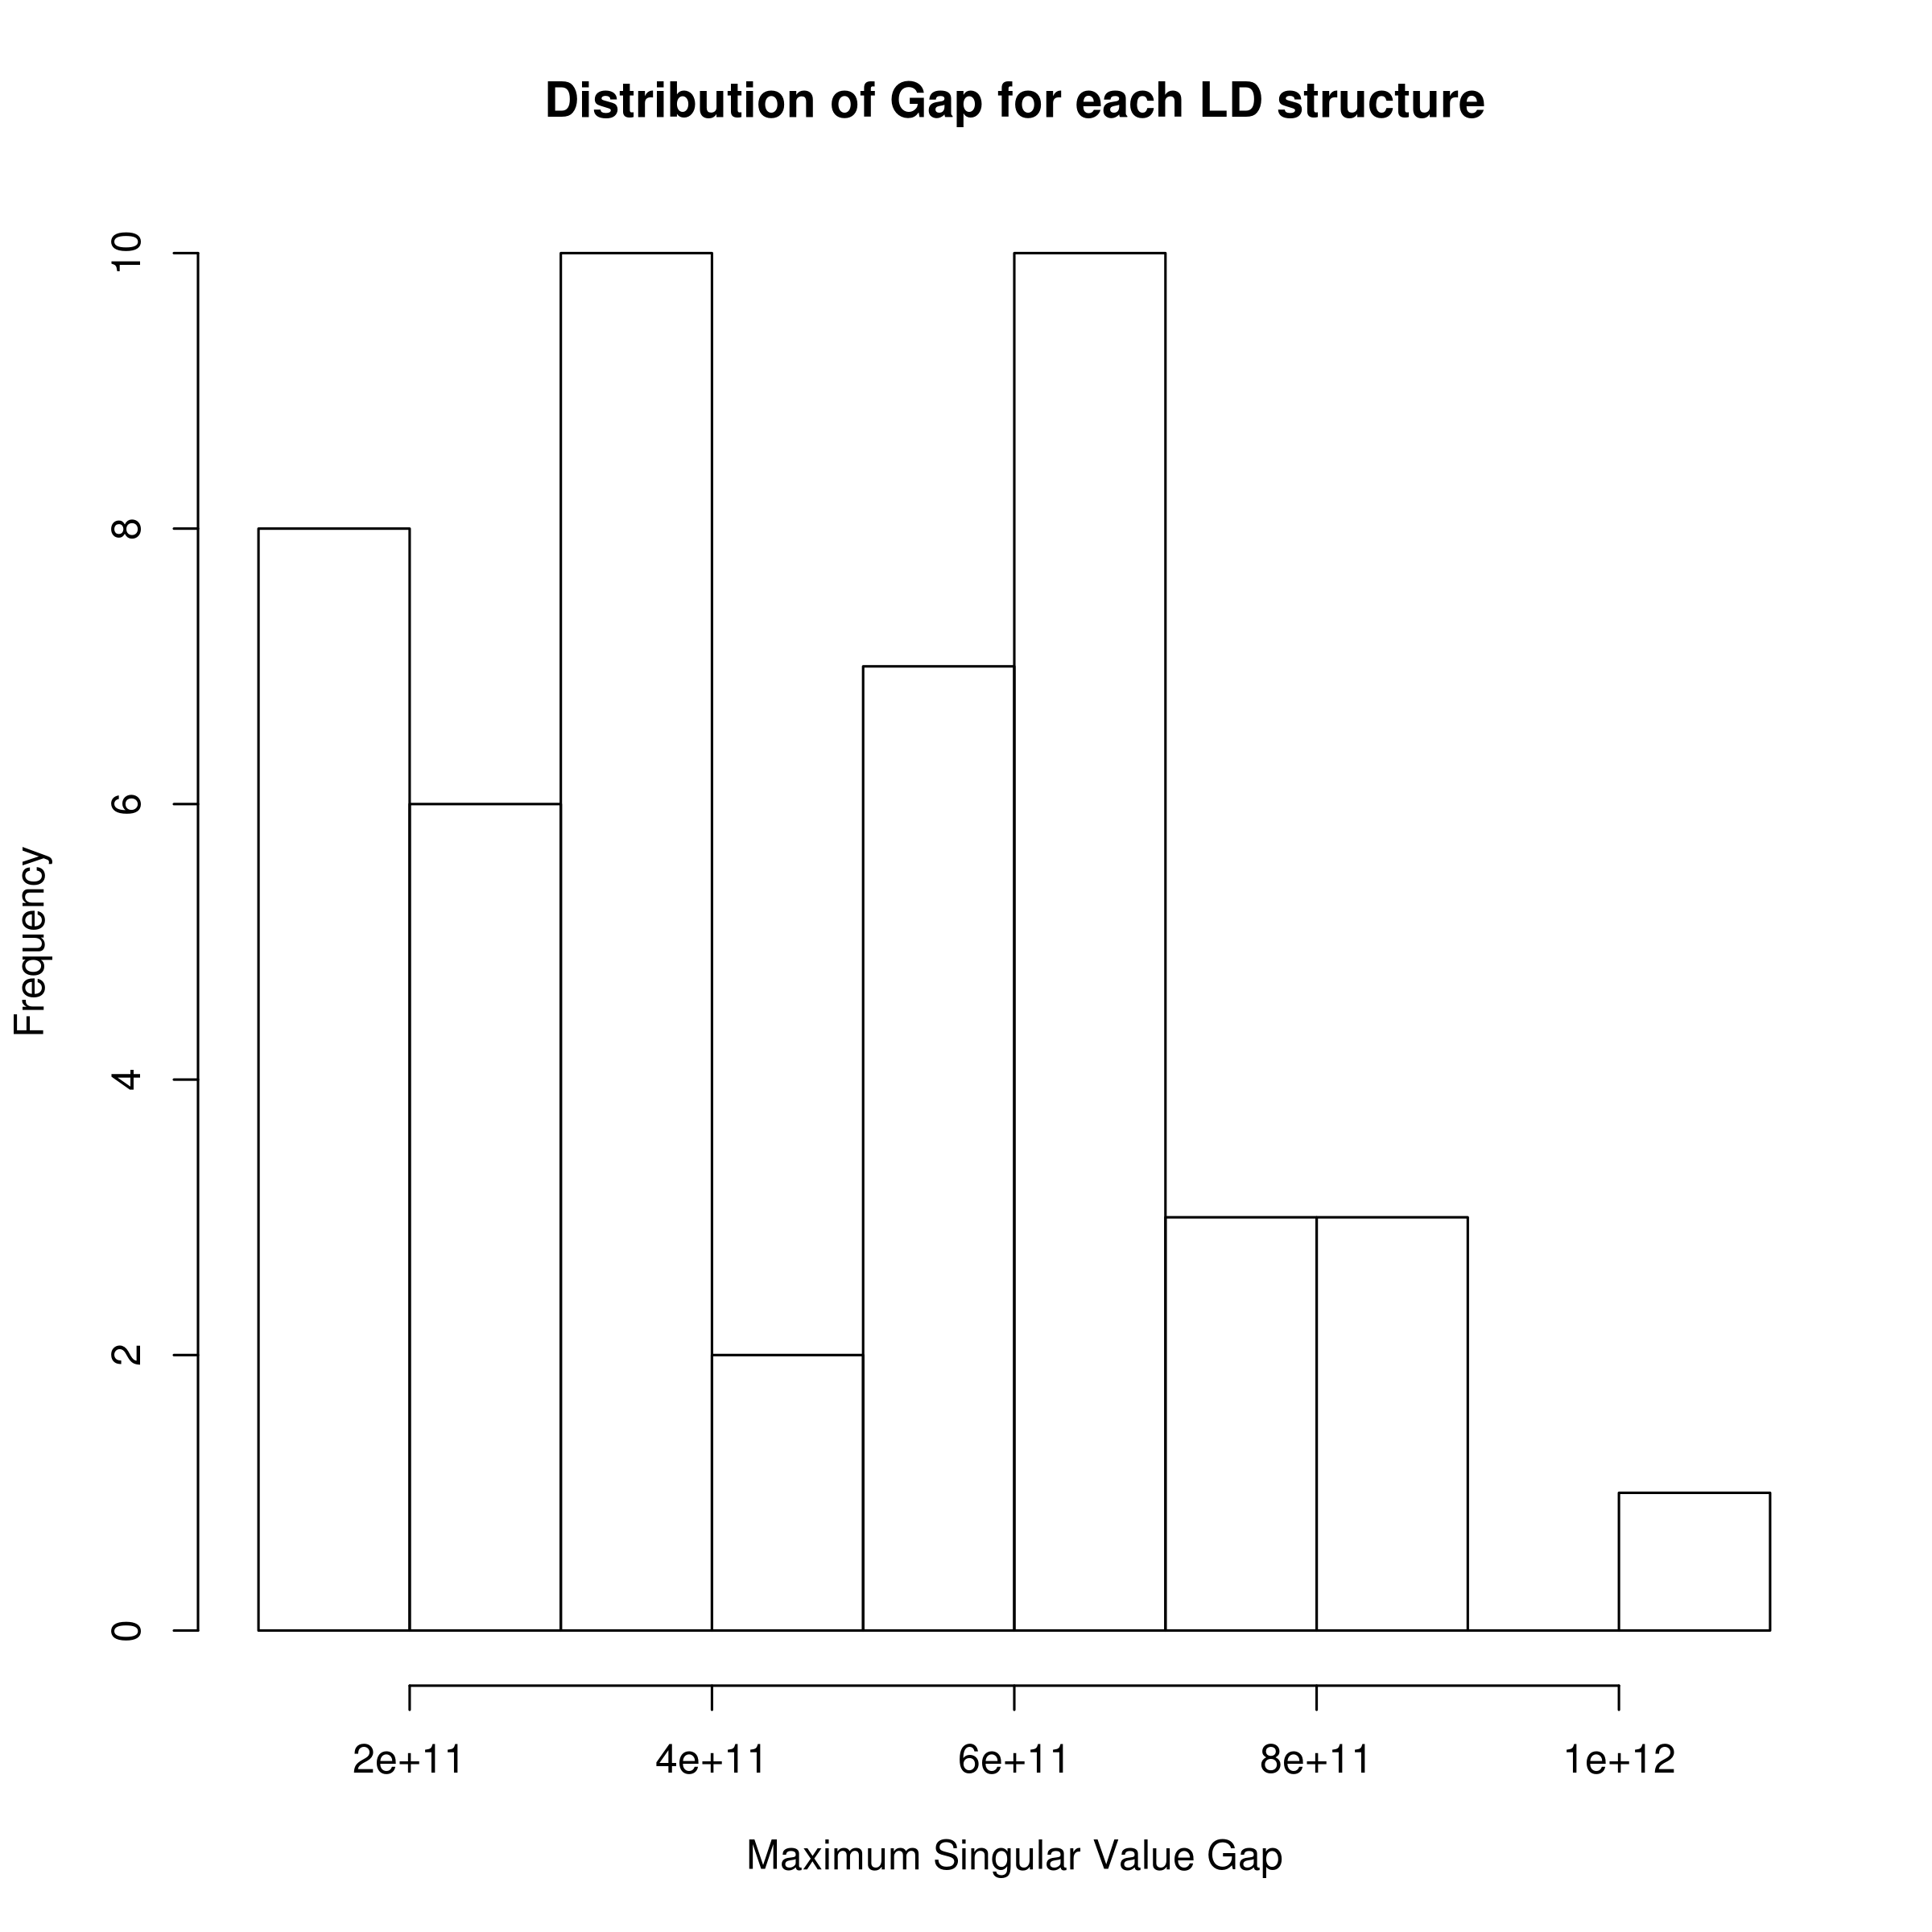
\includegraphics[width=0.5\textwidth]{figure/singular_value_distribution.png}
				\label{fig:singularValueDist}
				\vspace{-20pt}
			\end{figure}
			%\end{wrapfigure}
			
			By employing the \gls{tSVD} as a method for regularization, we were able to solve the ill-posed \cref{eq:shrekEq}, and obtain the estimated heritability.
						
		\subsection{Comparing with \glsentrylong{ldsc}}
			% main difference 
			Conceptually, the fundamental hypothesis of \gls{ldsc} and our algorithm were quite different.
			\gls{ldsc} were based on the ``global'' inflation of test statistic and its relationship to the \gls{LD} pattern.
			\gls{ldsc} hypothesize that the larger the \gls{LD} score, the more likely will the \gls{SNP} be able to ``tag'' the causal \gls{SNP} and the heritability can then be estimated through the regression between the \gls{LD} score and the test statistic.
			
			On the other hand, our algorithm focuses more on the per-\gls{SNP} level.
			Our main idea was that the individual test statistic of each \glspl{SNP} is a combination of its own effect and effect from \glspl{SNP} in \gls{LD} with it. 
			Thus, based on this concept, our algorithm aimed to ``remove'' the inflation of test statistic introduced through the \gls{LD} between \glspl{SNP} and the heritability can be calculated by adding the test statistic of all \glspl{SNP} after ``removing'' the inflation. 
			
			Mathematically, the calculation of \gls{ldsc} and our algorithm were also very different. 
			\gls{ldsc} take the sum of all $R^2$ within a 1cM region as the LD score and regress it against the test statistic to obtain the slope and intercept which represent the heritability and amount of confounding factors respectively. 
			In their model, \gls{ldsc} assume that each \glspl{SNP} will explain the same portion of heritability
			\begin{align}
			 \mathrm{Var}(\beta)&=\frac{h^2}{M}\boldsymbol{I}\\
			 M &= \text{number of SNPs}\notag\\
			 \beta &= \text{vector containing per normalized genotype effect sizes}\notag\\
			 I &= \text{identity matrix}\notag\\
			 h^2 &= \text{heritability}\notag
			\end{align}
			
			As for our algorithm, the whole \gls{LD} matrix were used and inverted to decompose the \gls{LD} from the test statistic. 
			There were no assumption of the amount of heritability explained by each \glspl{SNP}. 
			However, our algorithm does assumed that the null should be 1 and therefore cannot detect the amount of confounding factors. 
					
	\section{Assessing the Performance of Our Algorithm}
	\label{sec:shrekSim}
		First, we would like to test how well our algorithm works for heritability estimation under different scenarios.
		To account for different genetic architecture, we varies the heritability of the trait, the number of causal \glspl{SNP} and the genotypes(therefore varies the \gls{LD} pattern) during the quantitative trait simulation.
		
		\subsection{Sample Size}
		One important consideration in our simulation was the number of sample simulated. 
		The sample size was the most important parameter in determining the standard error of the heritability estimation. 
		As sample size increases, study will be more representative of the true population. 
		The increased number of information also means a better estimation of parameters, therefore a smaller \acrfull{se}.
		% awk -F "\t" '{print $2"\t"$9}' full | uniq | sed -e 's/[^0-9[:space:]]//g' | awk '{for(i=2;i<=NF;++i)j+=$i; print $1" "j; j=0}' | sort | uniq  %script for text mining
		Based on information from \gls{GWAS} catalog\citep{Welter2014}, we calculate the sample size distribution using simple text mining and exclude studies with conflicting sample size information in multiple entries. 
		The average sample size for all \gls{GWAS} recorded on the \gls{GWAS} catalog was 7,874, with a median count of 2,506 and a lower quartile at 940 (\cref{fig:gwasCata}). 
		We argue that if the algorithm works for studies with a small sample size (e.g lower quartile sample size), then it should perform even better when the sample size is larger. 
		Thus, we only simulate 1,000 samples in our simulation, which roughly represent the lower quartile sample size range.
		
		\begin{wrapfigure}{R}{8cm}
			\centering
			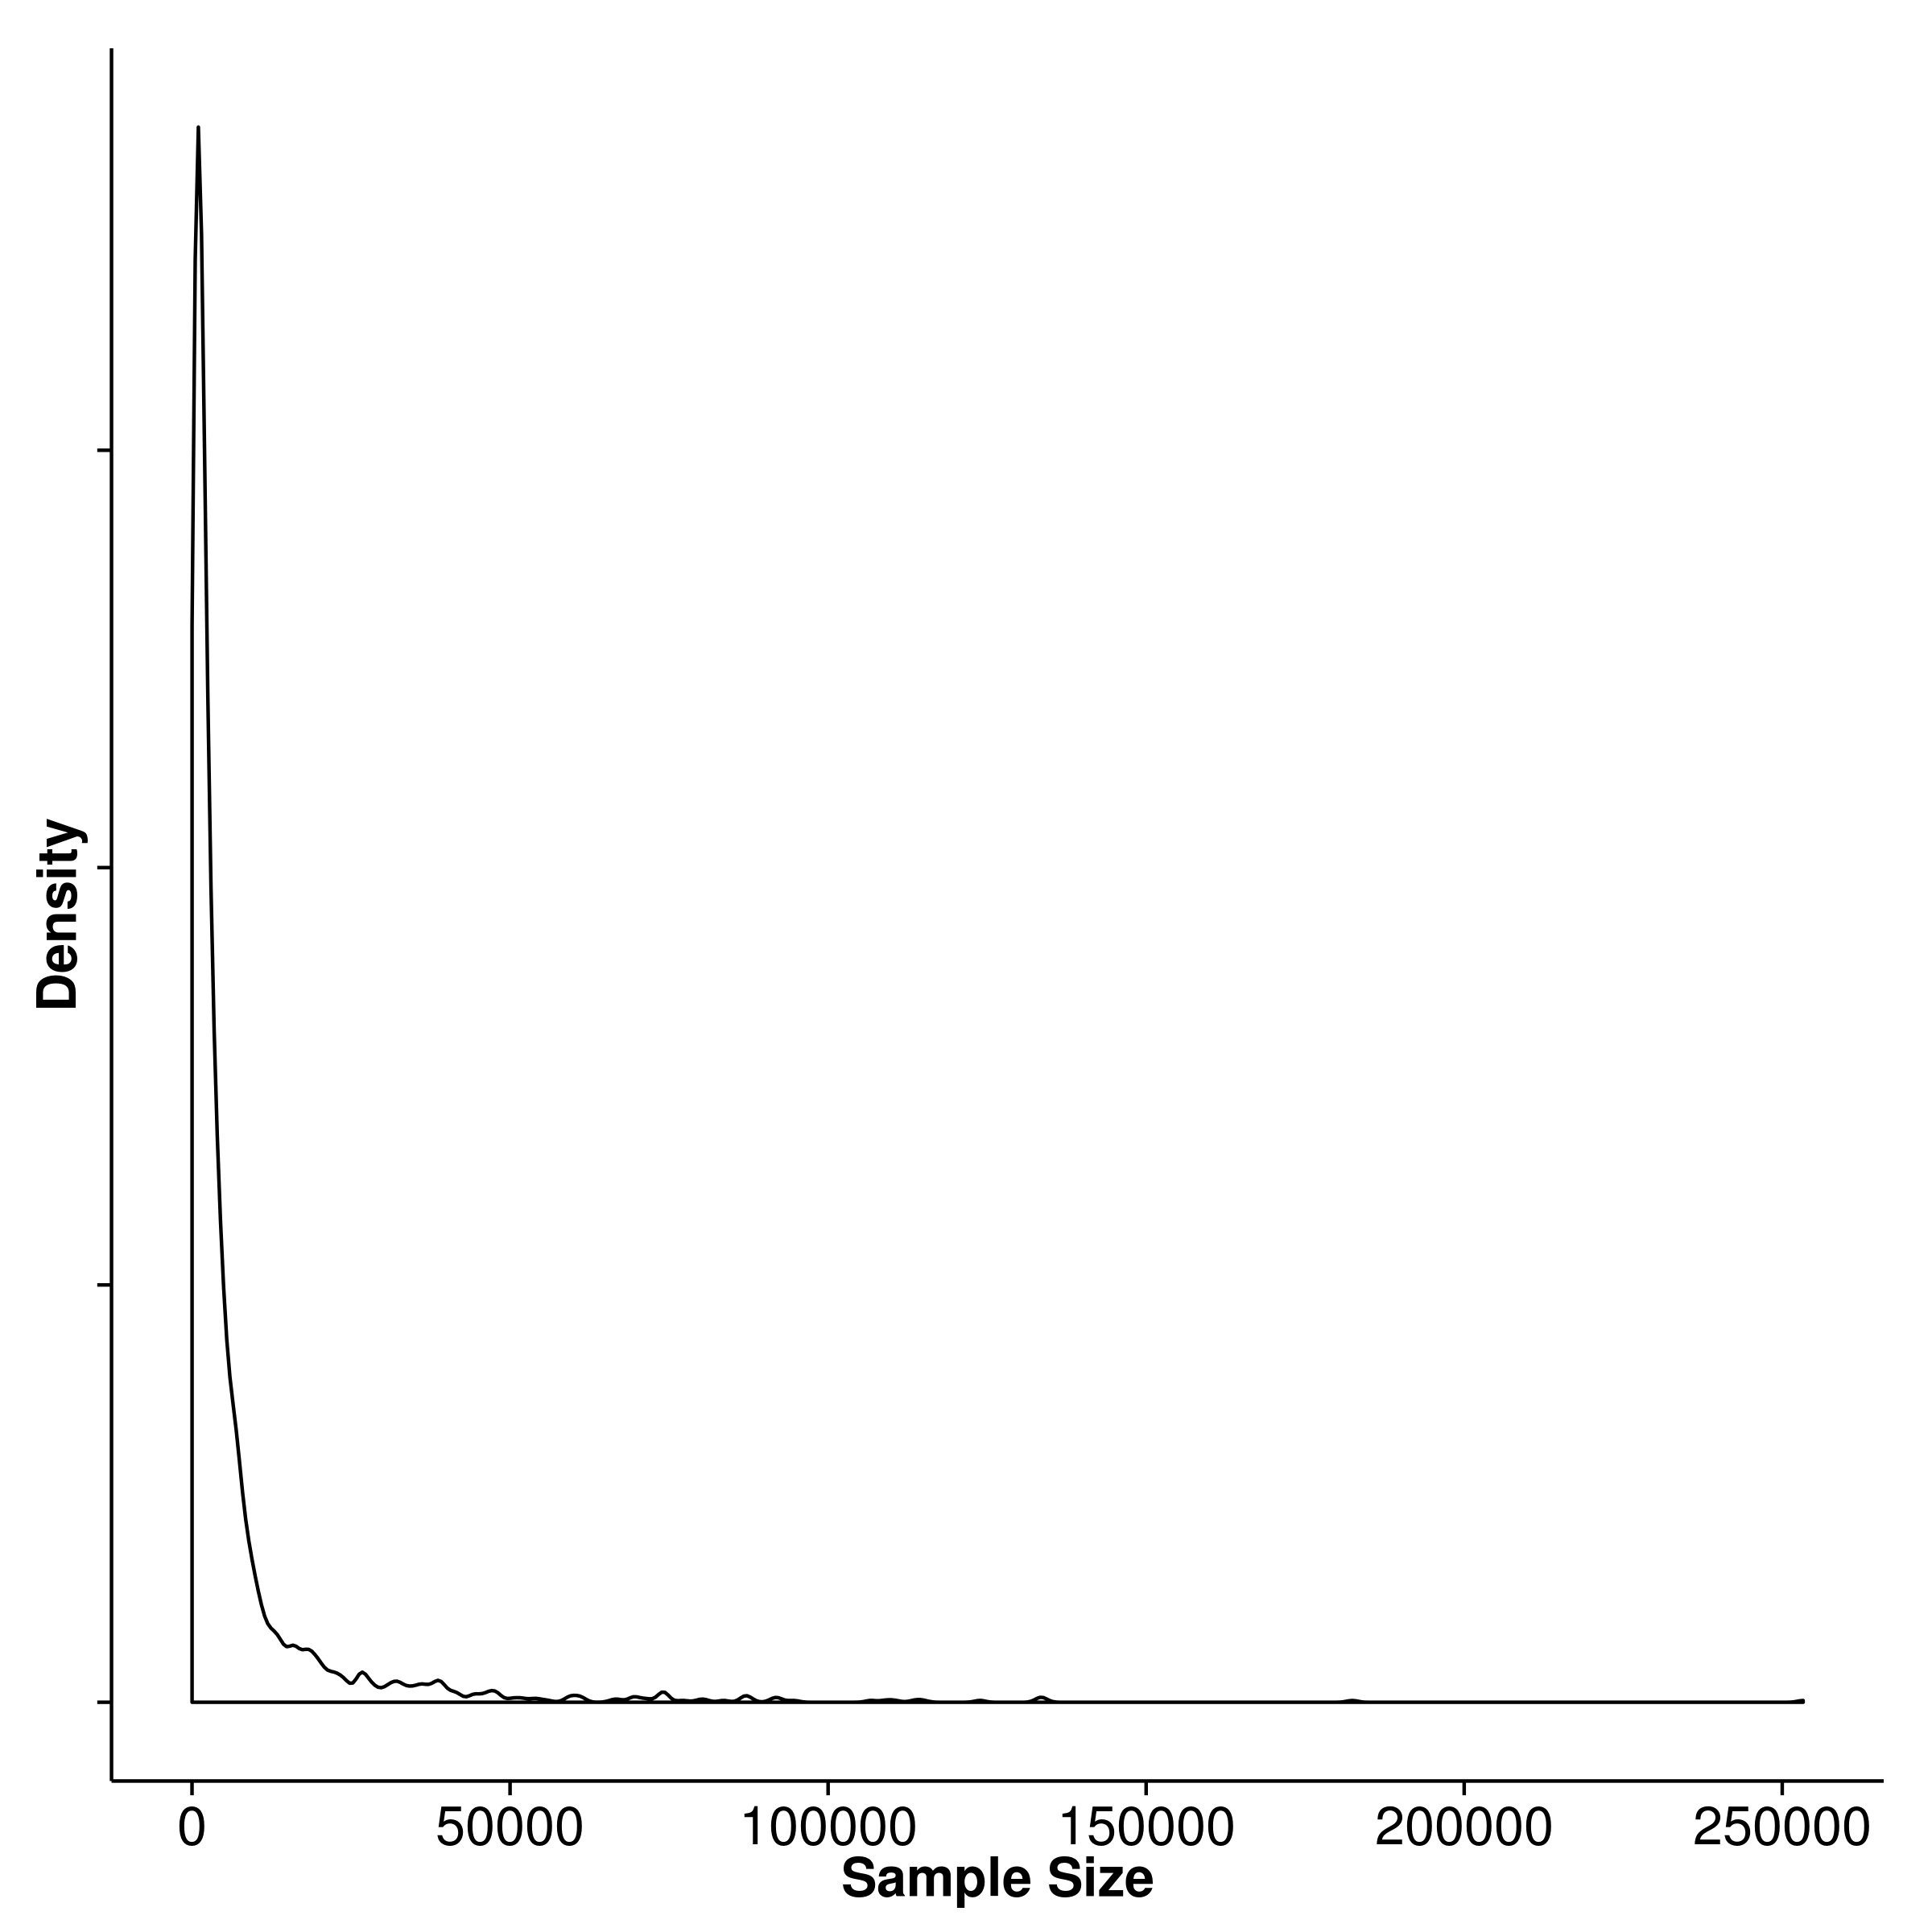
\includegraphics[width=0.5\textwidth]{figure/gwasSampleSize.png}
			\caption[GWAS Sample Size distribution]{
				\gls{GWAS} sample size distribution.
				}
			\label{fig:gwasCata}
		\end{wrapfigure}
		
		\subsection{Number of SNPs in Simulation}
		Another consideration in the simulation was the number of \glspl{SNP} included.
		In a typical \gls{GWAS} study, there are usually a larger number of \glspl{SNP} when compared to the sample size. 
		Fr example, in the \gls{pgc} \glng{scz} \gls{GWAS}, more than 9 million \glspl{SNP} were included, with around 700,000 \glspl{SNP} on chromosome 1.
		Although it would be idea to simulate 700,000 \glspl{SNP} in our simulation, the time required for simulating the samples will become unrealistic.
		
		As the number of \glspl{SNP} simulated grow, more time were required for the simulation of samples and more calculation will be required.
		Moreover, the increasing number of \glspl{SNP} will lead to increased size of the \gls{LD} matrix, requiring a long time for the inverse of the matrix.
		In reality, this should not be a real problem as one typically only calculate the heritability of the data set once and the speed of the algorithm is still relatively fast. 
		However, in the case of simulation where we would like to repeat the same analysis many times, the small increment of time will lead to an escalation in total simulation time, making the simulation infeasible. 
		To compromise, we simulate a total of 50,000 \glspl{SNP} from chromosome 1 as a balance between run time of simulation and the total \glspl{SNP} simulated.
		
		\subsection{Genetic Architecture}
		Of all simulation parameter, the genetic architecture was the most complicated and important parameter. 
		The \gls{LD} pattern, the number of causal \glspl{SNP}, the effect size of the causal \glspl{SNP} and the heritability of the trait were all important factors contribute to the genetic architecture of a trait. 
		
		First and foremost, because the aim of the algorithm was to estimating the heritability of the trait, it is important that the algorithm works for traits from different heritability spectrum.
		We therefore simulate traits with heritability ranging from 0 to 0.9, with increment of 0.1.
		
		Secondly, in real life scenario, the ``causal'' variant might not be readily included on the \gls{GWAS} chip and were only ``tagged'' by \glspl{SNP} included on the \gls{GWAS} chip.
		However, to simplify our simulation, all ``causal'' variants were included in our simulation (e.g. perfectly ``tagged'')
		
		Thirdly, to obtain a realistic \gls{LD} pattern, we simulate the genotypes using the HAPGEN2 programme\citep{Su2011}, using the 1000 genome \gls{CEU} haplotypes as an input.
		In short, HAPGEN2 simulate new haplotypes as an imperfect mosaic of haplotpyes from a reference panel and the haplotypes that have already been simulated using the \textit{Li and Stephens} (LS) model of \gls{LD} \citep{Li2003}.
		In a typical \gls{GWAS} , one usually only have power in detecting ``common variants'', usually defined as variants with \gls{maf} $\ge 0.01$.
		We therefore only consider scenario with ``common'' variants and only use \glspl{SNP} with \gls{maf} $\ge0.1$ in the \gls{CEU} haplotypes as an input to HAPGEN2. 
		This will reduce the probability of having \glspl{SNP} with \gls{maf} $<0.01$ in the final simulated sample sets.
		
		Finally, we would like to simulate traits with different inheritance model such as oligogenic traits and polygenic traits.
		We therefore varies the number of causal \glspl{SNP} ($k$) with $k\in\{5, 10, 50, 100, 250, 500\}$.
		An important consideration in the simulation of causal \glspl{SNP} is the effect size distribution. 
		\citet{Orr1998} suggested that the exponential distribution can be used to approximate the genetic architecture of adaptation. 
		As a result of that, we used the exponential distribution with $\lambda=1$ as an approximation to the effect size distribution:
		\begin{align}
		\theta&=\mathrm{exp}(\lambda=1)\notag\\
		\beta&=\pm\sqrt{\frac{\theta \times h^2}{\sum \theta}}
		\label{eq:randomEffect}
		\end{align}
		with a random direction of effect.
		
		Given the normalized genotype as $\boldsymbol{X}$ and the simulated heritability as $h^2$, the phenotype can then be calculated as 
		\begin{align}
		\epsilon_i&\sim N(0,\sqrt{\mathrm{Var}(\boldsymbol{X\beta})\frac{1-h^2}{h^2}} )\notag\\
		\boldsymbol{\epsilon} &= (\epsilon_1,\epsilon_2,...,\epsilon_n)^t\notag\\
		\boldsymbol{y} &= \boldsymbol{X\beta}+\boldsymbol{\epsilon}
		\label{eq:simulationOfPhenotype}
		\end{align}
		
		The test statistics were then calculated using the plink programme \citep{Purcell2007} and input to our algorithm to estimate the heritability. 
		An independent 500 samples were simulated as a reference panel for the calculation of \gls{LD} matrix as in reality, we should not have the sample genotype for the construction of the \gls{LD} matrix. 
		The whole process will be repeated 50 times such that a distribution of the estimate can be obtained. 
		The whole simulation process can be viewed as follow:
		We simulate a large population of samples (e.g. $50\times1,000+500 = 50,500$) where 500 samples were randomly selected as a reference panel. 
		In the subsequent iteration of simulation, 1,000 samples were randomly selected from the population \textit{without replacement} and estimation were performed.
		We then simulate 10 different population and repeat the whole process.
		
		In summary:
		\begin{enumerate}
			\item Randomly select 50,000 \glspl{SNP} with \gls{maf}$>0.1$ from chromosome 1
			\item Simulate 500 samples using HAPGEN2 and used as a reference panel
			\item Randomly generate $k$ effect size with $k \in \{5,10,50,100,250,500\}$ following  \cref{eq:randomEffect}
			\item Randomly assign the effect size to $k$ \glspl{SNP}
			\item Simulate 1,000 samples using HAPGEN2 and calculate their phenotype according to \cref{eq:simulationOfPhenotype}
			\item Perform heritability estimation using our algorithm
			\item Repeat step 5-6 50 times
			\item Repeat step 1-7 10 times
		\end{enumerate}
		
		\section{Comparison with Other Programmes}
		It is also important for us to compare our algorithm to existing methods for the performance in estimating the narrow sense heritability.
		We would also like to extend the simulation to other conditions such as quantitative traits with extreme effect size distribution, case control studies and quantitative traits with extreme phenotype selections.
		
		Currently, the only other programme that is capable to estimate the narrow sense heritability using only test statistic is the \gls{ldsc} \citep{Bulik-Sullivan2015}. 
		On the other hand, \gls{gcta} \citep{Yang2011} is commonly considered as the golden standard for heritability estimation in \gls{GWAS} data. 
		Therefore, we choose to compare the performance of our algorithm to that of \gls{ldsc} and \gls{gcta}.
		It is important to note that as we are assessing the performance of the programme through controlled simulation, there should be little confounding factors. 
		For \gls{ldsc}, the default intercept estimation function allows it to estimate and correct for confounding factors with an increase in \gls{se}. 
		The simulation will therefore be unfair to \gls{ldsc} with intercept estimation, as the \gls{se} is increased yet there are little confounding factors for it to correct.
		Thus, we also simulate \gls{ldsc} with a fixed intercept (-{}-no-intercept) parameters to avoid bias against \gls{ldsc}.	
		
		\subsection{Simulation}
		We first repeated the whole simulation process in \cref{sec:shrekSim} by including \gls{gcta}, \gls{ldsc} with fixed intercept and \gls{ldsc} with intercept estimation on top of our algorithm. 
		The sample genotype was provided to \gls{gcta} for the calculation of the genetic relationship matrix and the estimation of heritability.
		On the other hand, the \gls{LD} score for \gls{ldsc} were calculated using the same simulated reference panel as our algorithm to simulate conditions where the sample genotype was not available.
		So the simulation follows the following procedure:
		
		\begin{enumerate}
			\item Randomly select 50,000 \glspl{SNP} with \gls{maf}$>0.1$ from chromosome 1
			\item Simulate 500 samples using HAPGEN2 and used as a reference panel
			\item Randomly generate $k$ effect size with $k \in \{5,10,50,100,250,500\}$ following  \cref{eq:randomEffect}
			\item Randomly assign the effect size to $k$ \glspl{SNP}
			\item Simulate 1,000 samples using HAPGEN2 and calculate their phenotype according to \cref{eq:simulationOfPhenotype}
			\item Perform heritability estimation using our algorithm, \gls{gcta}, \gls{ldsc} with fixed intercept and \gls{ldsc} with intercept estimation.
			\item Repeat step 5-6 50 times
			\item Repeat step 1-7 10 times
		\end{enumerate}
		
		\subsection{Extreme Effect Size}
		On top of the original quantitative trait simulation, another condition we were interested in was the performance of the algorithms when there is a small amount of \glspl{SNP} with a much larger effect size.
		This can be observed in disease such as %HERE
		
		To simulate extreme effect size, we consider scenarios where $m$ \glspl{SNP} accounts 50\% of all the effect size with $m\in\{1,5,10\}$.
		The effect size was then calculated as
		\begin{align}
		\beta_{eL} &= \pm\sqrt{\frac{0.5h^2}{m}} \notag\\
		\beta_{eS} &= \pm\sqrt{\frac{0.5h^2}{100-m}} \notag\\
		\beta &= \{\beta_{eL}, \beta_{eS}\}
		\label{eq:extremEffect}
		\end{align}
		The effect size were then randomly assigned to 100 causal \glspl{SNP} and phenotype will be calculated as in \cref{eq:simulationOfPhenotype}.
		The simulation procedure then becomes
		\begin{enumerate}
			\item Randomly select 50,000 \glspl{SNP} with \gls{maf}$>0.1$ from chromosome 1
			\item Simulate 500 samples using HAPGEN2 and used as a reference panel
			\item Randomly generate 100 effect size where $m$ has extreme effect, following \cref{eq:extremEffect}, with $m\in\{1,5,10\}$
			\item Randomly assign the effect size to 100 \glspl{SNP}
			\item Simulate 1,000 samples using HAPGEN2 and calculate their phenotype according to \cref{eq:simulationOfPhenotype}
			\item Perform heritability estimation using our algorithm, \gls{ldsc} with fixed intercept, \gls{ldsc} with intercept estimation and \gls{gcta}
			\item Repeat step 5-6 50 times
			\item Repeat step 1-7 10 times
		\end{enumerate}
		
		\subsection{Case Control Studies}
		The simulation of case control studies was similar to the simulation of quantitative trait. 
		However, there were two additional parameters to consider: the population prevalence and the observed prevalence.
		These parameters were required to simulate the samples under a liability model for case control studies.

		Although there were only two additional parameter, it is significantly more challenging for to simulate when compared to the simulation of quantitative traits.
		It is mainly because of the number of samples required to simulate adequate samples under the liability threshold model.
		Take for example, if one like to simulate a trait with population prevalence of $p$ and observed prevalence of $q$ and would like to have $n$ cases in total, one will have to simulate $\min(\frac{n}{p}, \frac{n}{q})$ samples.
		Considering the scenario where the observed prevalence is 50\%, the population prevalence is 1\%, if we want to simulate 1,000 cases, a minimum of 100,000 samples will be required.
		
		Given limited computer resources, it will be infeasible for us to simulate 1,000 cases with 50,000 \glspl{SNP} when the population prevalence is small.
		To simplify the simulation and reduce the burden of computation, we limited the observed prevalence to 50\% and varies the population prevalence $p$ such that $p\in\{0.5, 0.1, 0.05, 0.01\}$.
		Most importantly, we reduce the number of \glspl{SNP} simulated to 5,000 on chromosome 22 instead of 50,000 \glspl{SNP} on chromosome 1. 
		The change from chromosome 1 to chromosome 22 allow us to reduce the number of \glspl{SNP} without changing much of the \gls{SNP} density. 
		We acknowledged that the current simulation was relatively brief, however, it should serves as a prove of concept simulation to study the performance of the algorithms under the case control scenario.
		
		In the case control simulation, we randomly select 5,000 \glspl{SNP} from chromosome 22 with \gls{maf} $\ge0.1$ in the \gls{CEU} haplotypes as an input to HAPGEN2. 
		We then randomly select 100 \glspl{SNP} with effect size simulated based on \cref{eq:randomEffect}.
		In order to simulate a case control samples with 1,000 cases, we then simulate $\frac{1,000}{p}$ samples and calculate their phenotype using \cref{eq:simulationOfPhenotype}.
		The phenotype was then standardized and cases were defined as sample with phenotype passing the liability threshold with respect to $p$.
		An equal amount of samples were then randomly selected from samples with phenotype lower than the liability threshold and defined as controls.
			
		Finally, the case control simulation were performed as:
		\begin{enumerate}
			\item Randomly select 5,000 \glspl{SNP} with \gls{maf}$>0.1$ from chromosome 22
			\item Simulate 500 samples using HAPGEN2 and used as a reference panel
			\item Randomly generate 100 effect size following  \cref{eq:randomEffect}
			\item Randomly assign the effect size to 100 \glspl{SNP}
			\item Simulate $\frac{1,000}{p}$ samples using HAPGEN2 and calculate their phenotype according to \cref{eq:simulationOfPhenotype}
			\item Define case control status using the liability threshold and randomly select same number of case and controls for subsequent simulation
			\item Perform heritability estimation using our algorithm, \gls{ldsc} with fixed intercept, \gls{ldsc} with intercept estimation and \gls{gcta}
			\item Repeat step 5-7 50 times
			\item Repeat step 1-8 10 times
		\end{enumerate}
		
		\subsection{Extreme Phenotype Selection}
		The simulation of extreme phenotype selection was the same as the quantitative trait simulation. 
		The only difference being that instead of using all samples for heritability estimation, we only use the extreme 10\% of samples among the population for the heritability estimation.
		In brief, instead of simulating 1,000 samples, we simulate 5,000 samples following the exact procedure in the quantitative trait simulation with random effect size.
		However, after simulation of the phenotype using \cref{eq:simulationOfPhenotype}, we standardize the phenotype and only select the top 10\% and bottom 10\% samples (500 samples each) from the sample distribution.
		We then perform the same simulation procedure as in the quantitative trait simulation with random effect size.
		
		It was noted that the extreme phenotype selection were not supported by the \gls{ldsc} and \gls{gcta}.
		To allow comparison in such scenario, we apply the extreme phenotype adjustment from \citet{Sham2014} to the estimation obtained from \gls{ldsc} and \gls{gcta}.
		
	\section{Result}
		The heritabilibty estimation were implemented in \gls{shrek} and is available on \url{https://github.com/choishingwan/shrek}.  
		\subsection{Performance}
		
		To study the performance of \gls{shrek} and \gls{ldsc} in comparison to \gls{gcta}, we performed a variety of simulations to model scenarios with different number of causal \glspl{SNP}, different effect size distribution and different type of traits. 
		
		First, we examined the performance of the algorithms under the quantitative trait scenario. 
		In the quantitative trait scenario, we varies the number of causal \glspl{SNP} and either assigned an equal effect size to each causal \glspl{SNP} or assigned a per-allele effect sizes drawn from the squared root of the exponential distribution with $\lambda=1$.
		
		\subsection{Quantitative Trait Simulation with Equal Effect Size}
		% QT Equal Effect
		
		\begin{figure}
			\centering
			\subfloat[SHREK]{
				\scalebox{.4}{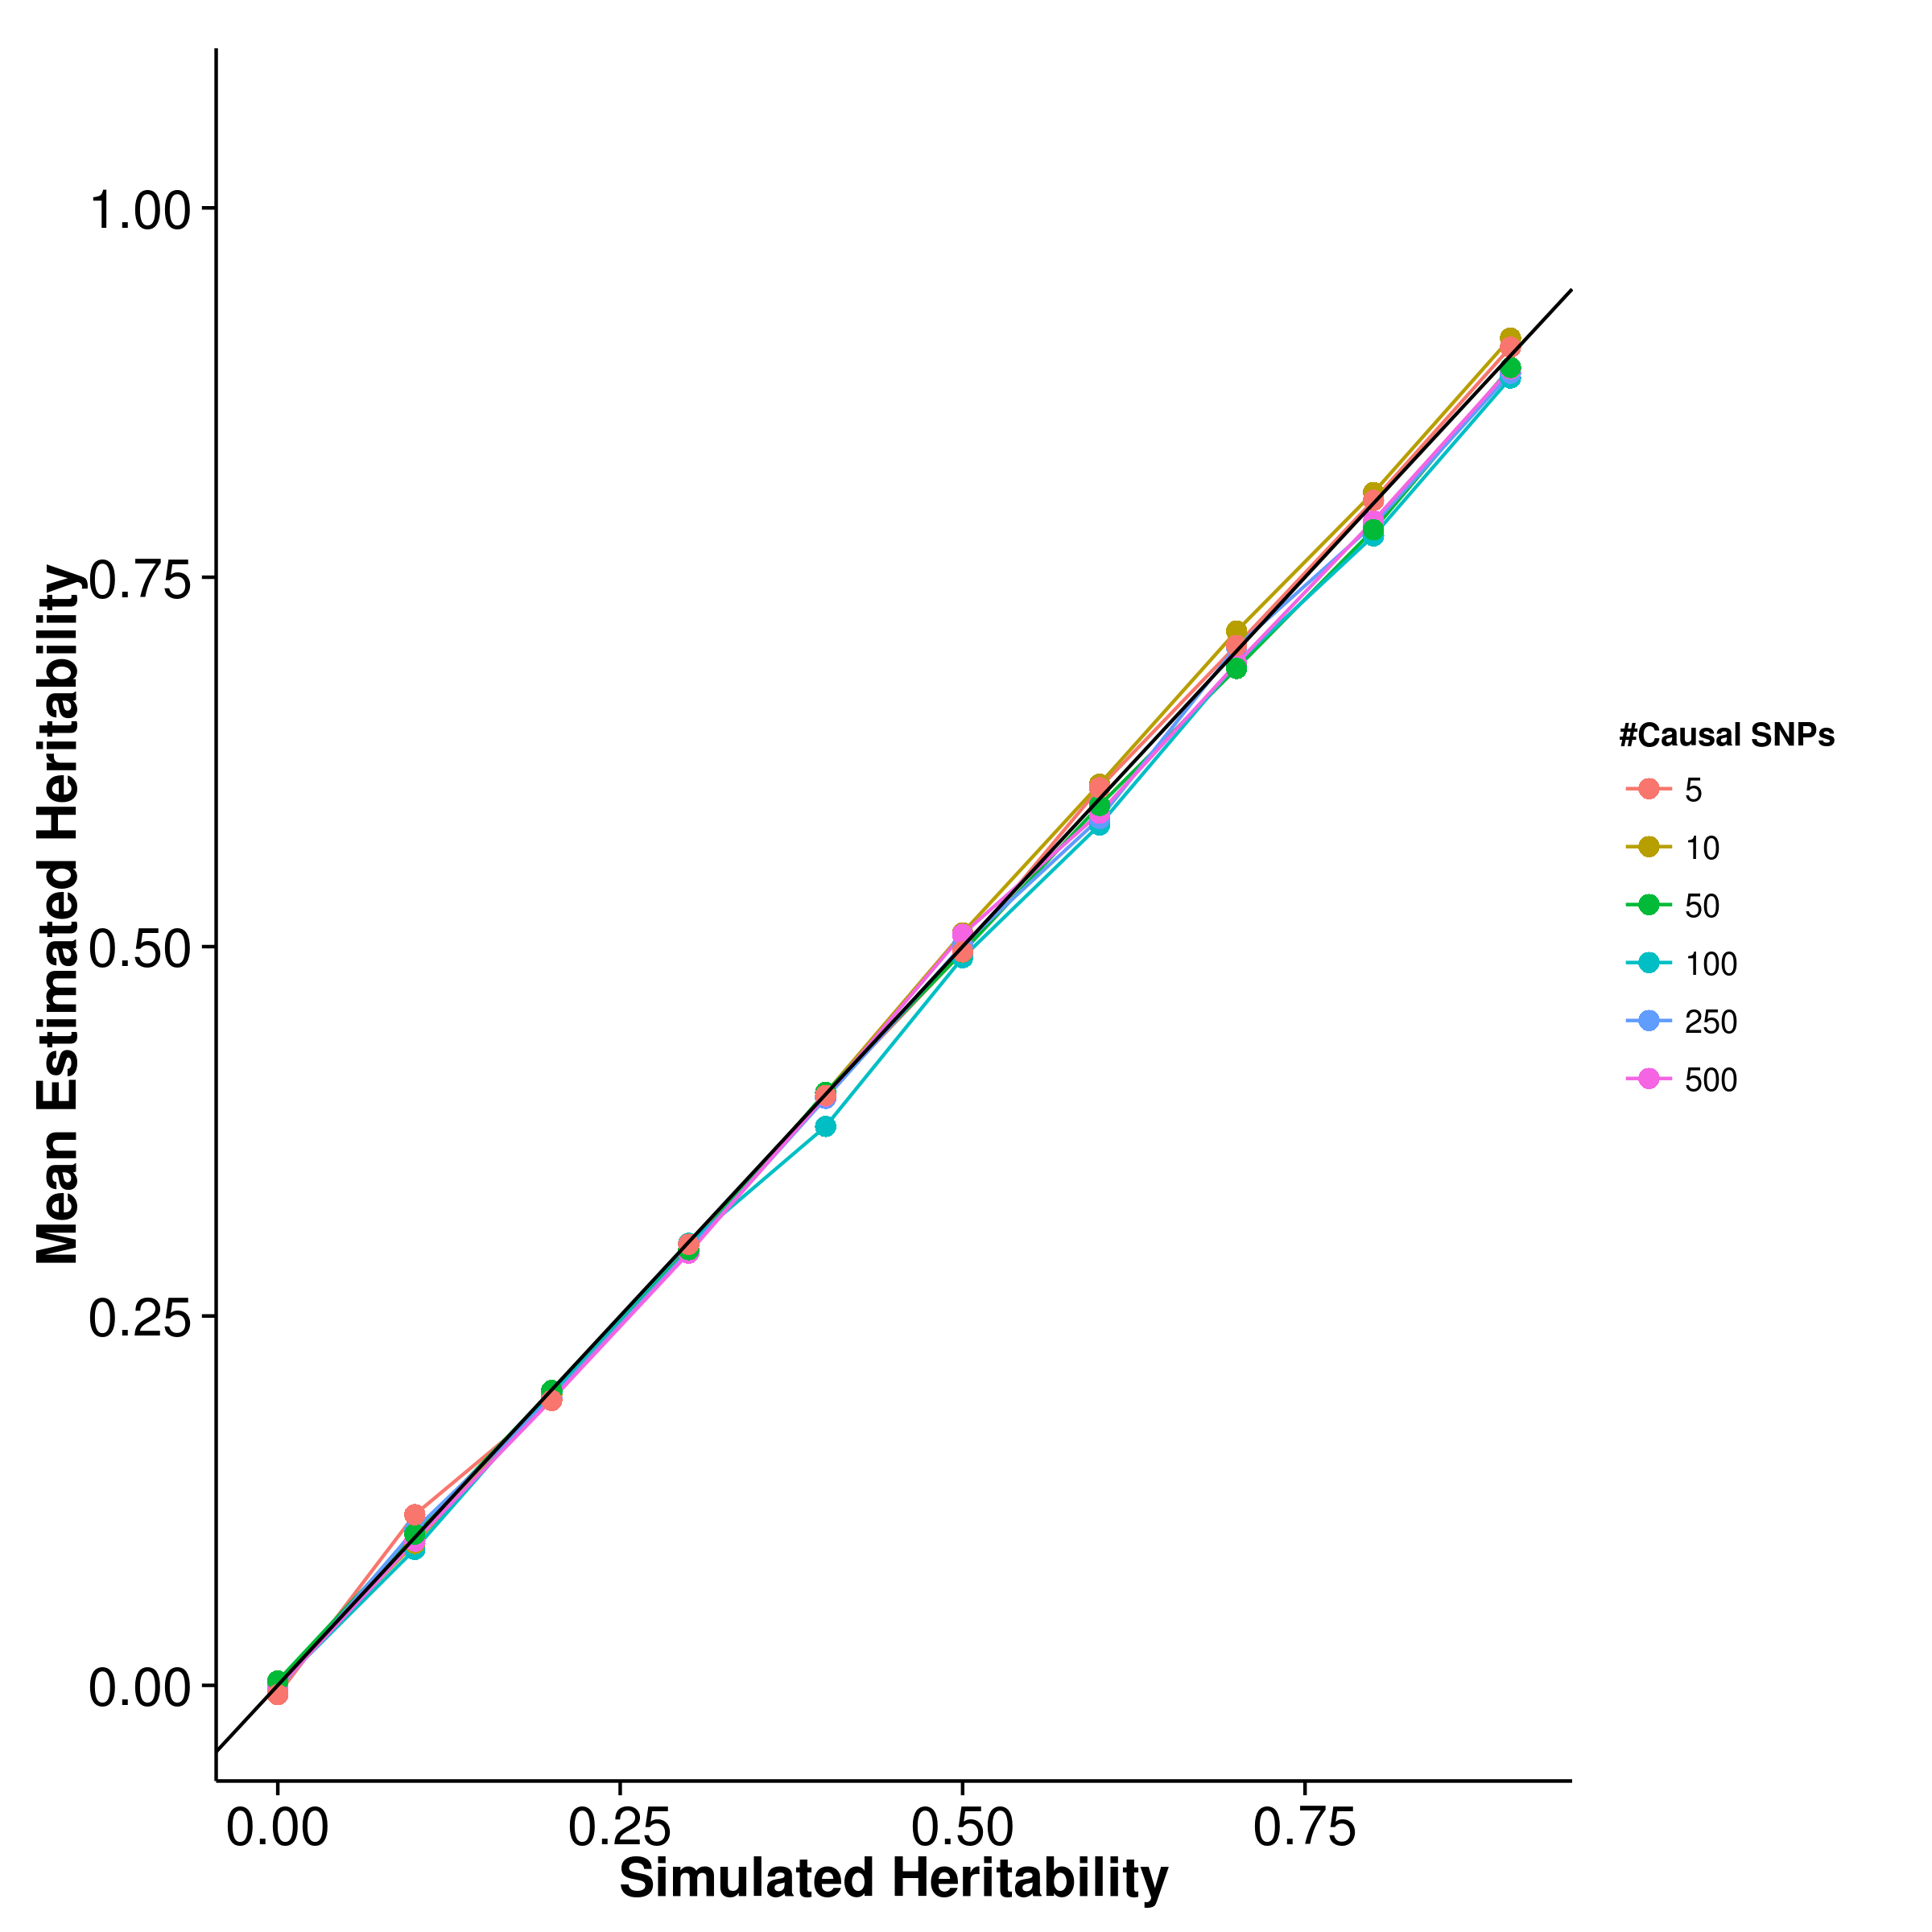
\includegraphics{figure/he_summary/equal/shrek_Qt_Equal_mean.png}}
				\label{fig:shrekQtEqualMean}
			}
			\subfloat[GCTA]{
				\scalebox{.4}{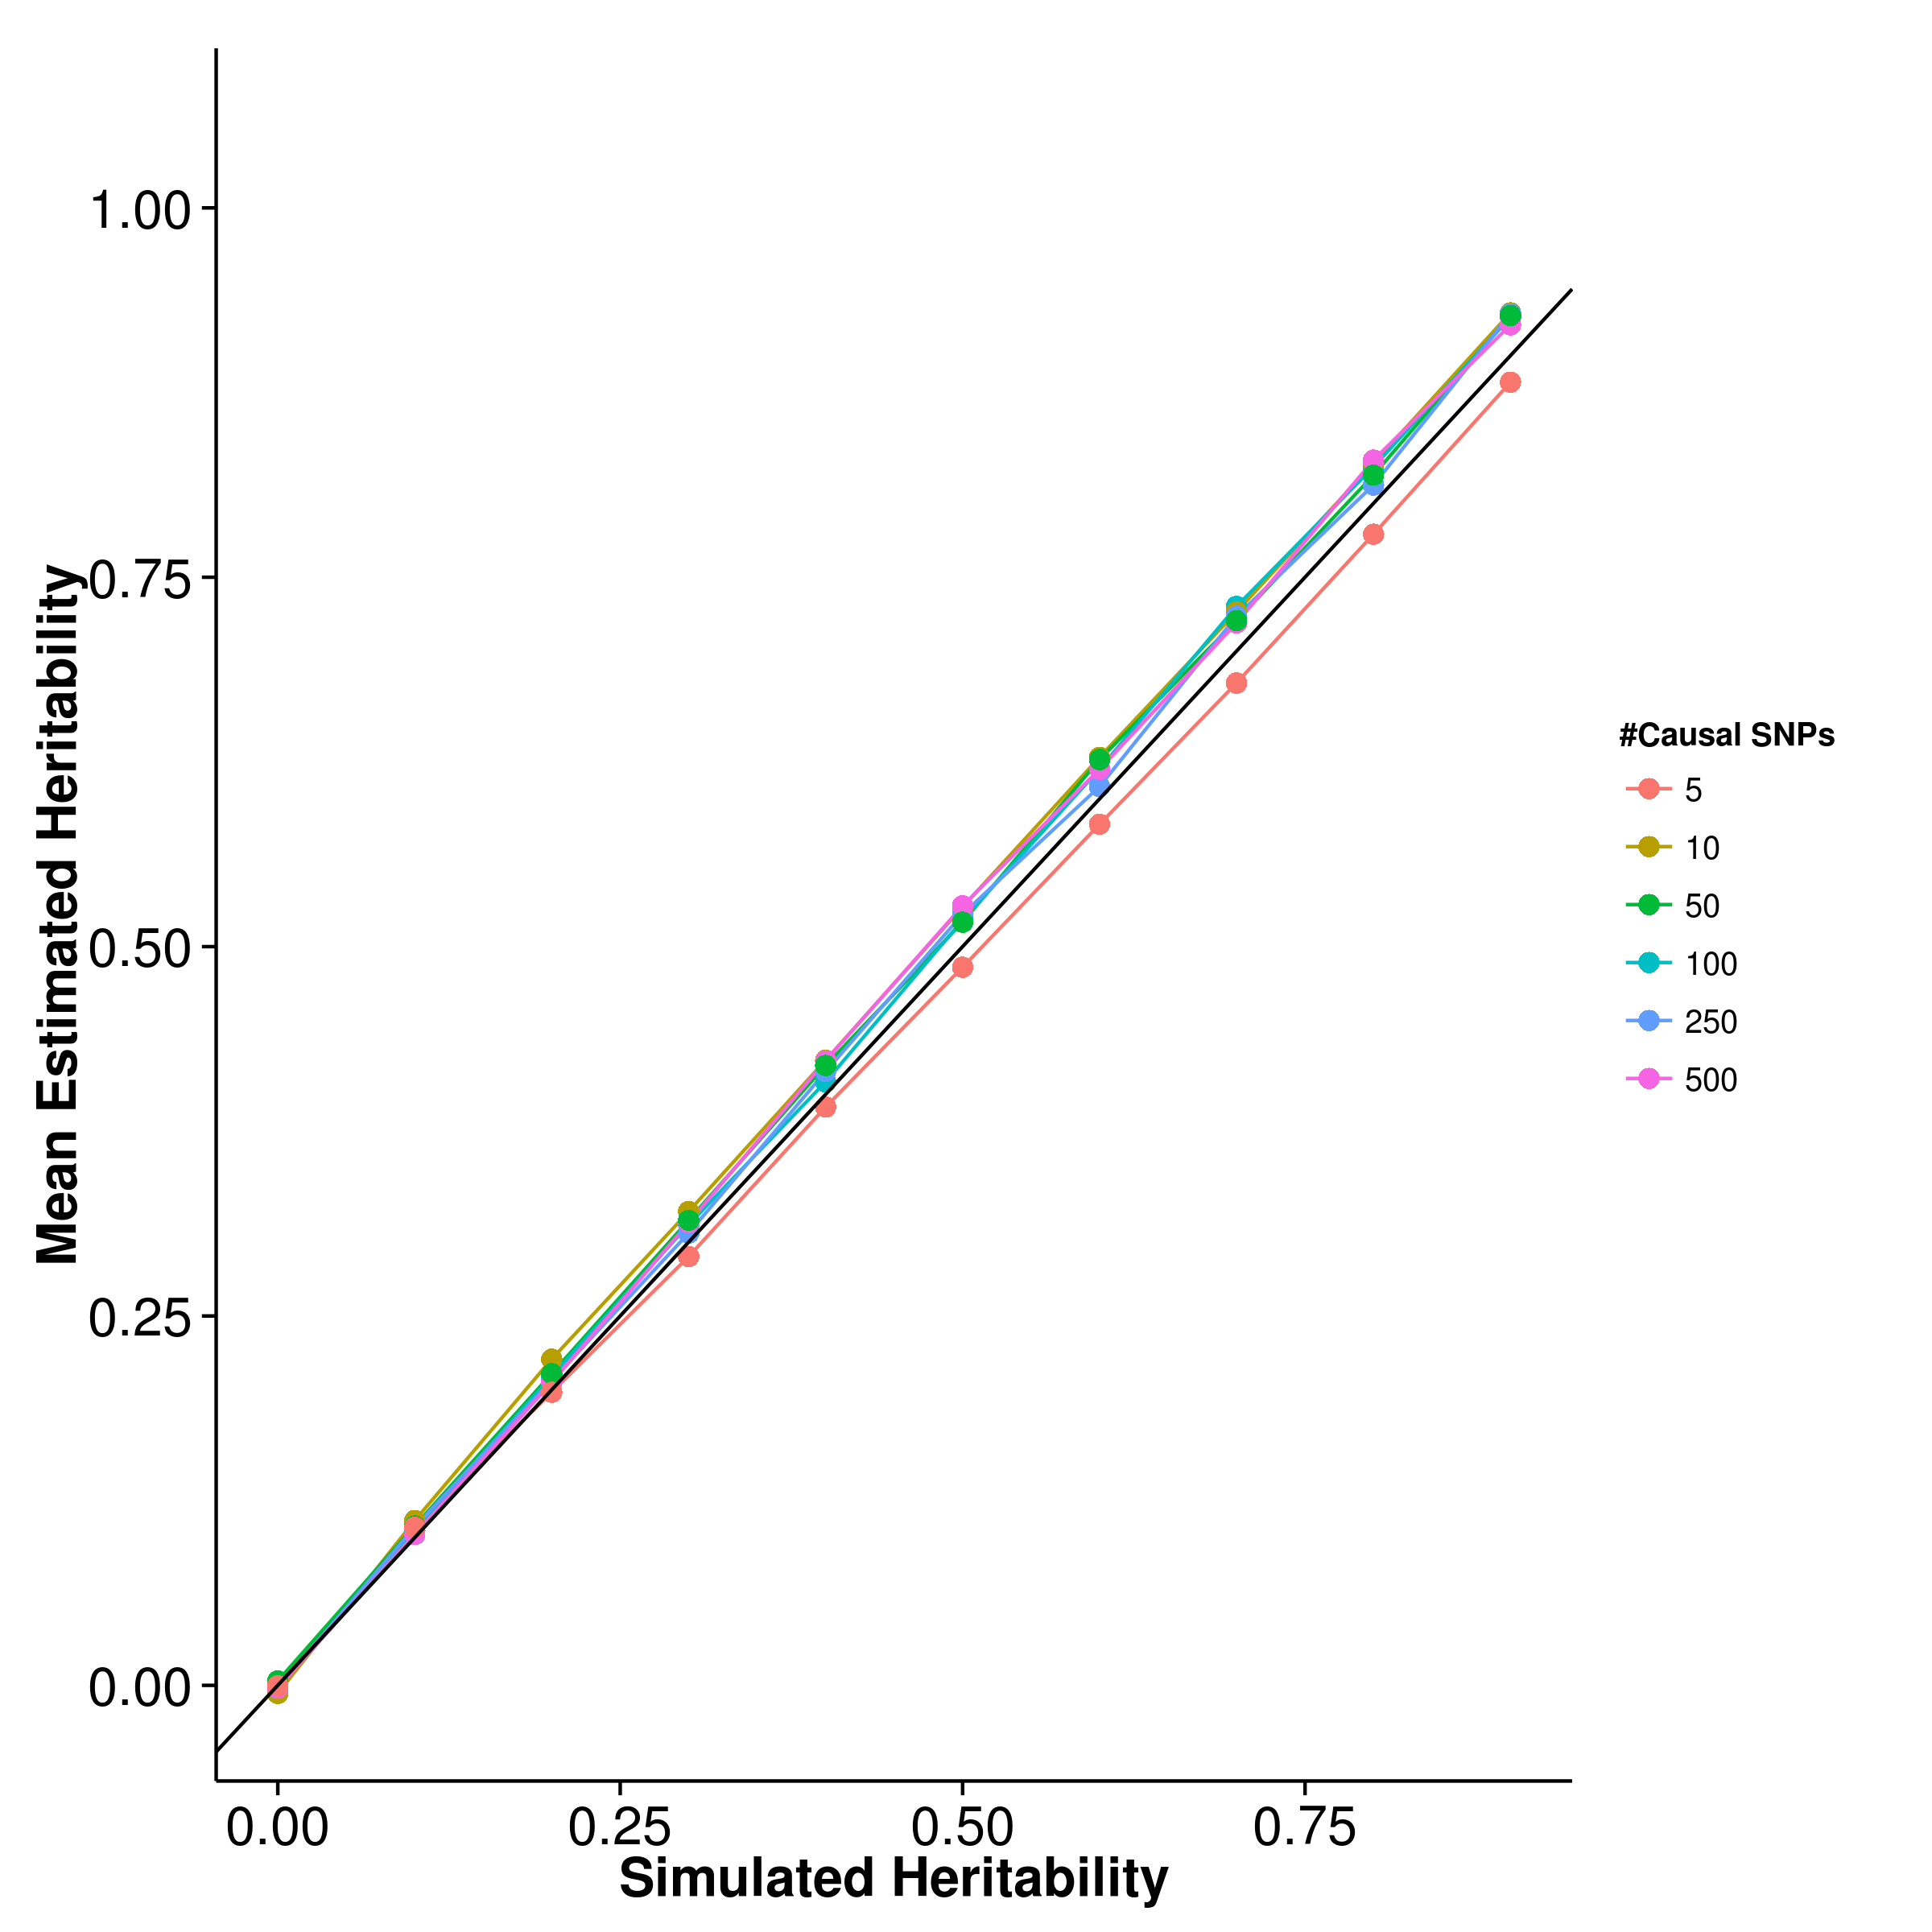
\includegraphics{figure/he_summary/equal/gcta_Qt_Equal_mean.png}}
				\label{fig:gctaQtEqualMean}
			}\\
			\subfloat[LDSC with fix intercept]{
				\scalebox{.4}{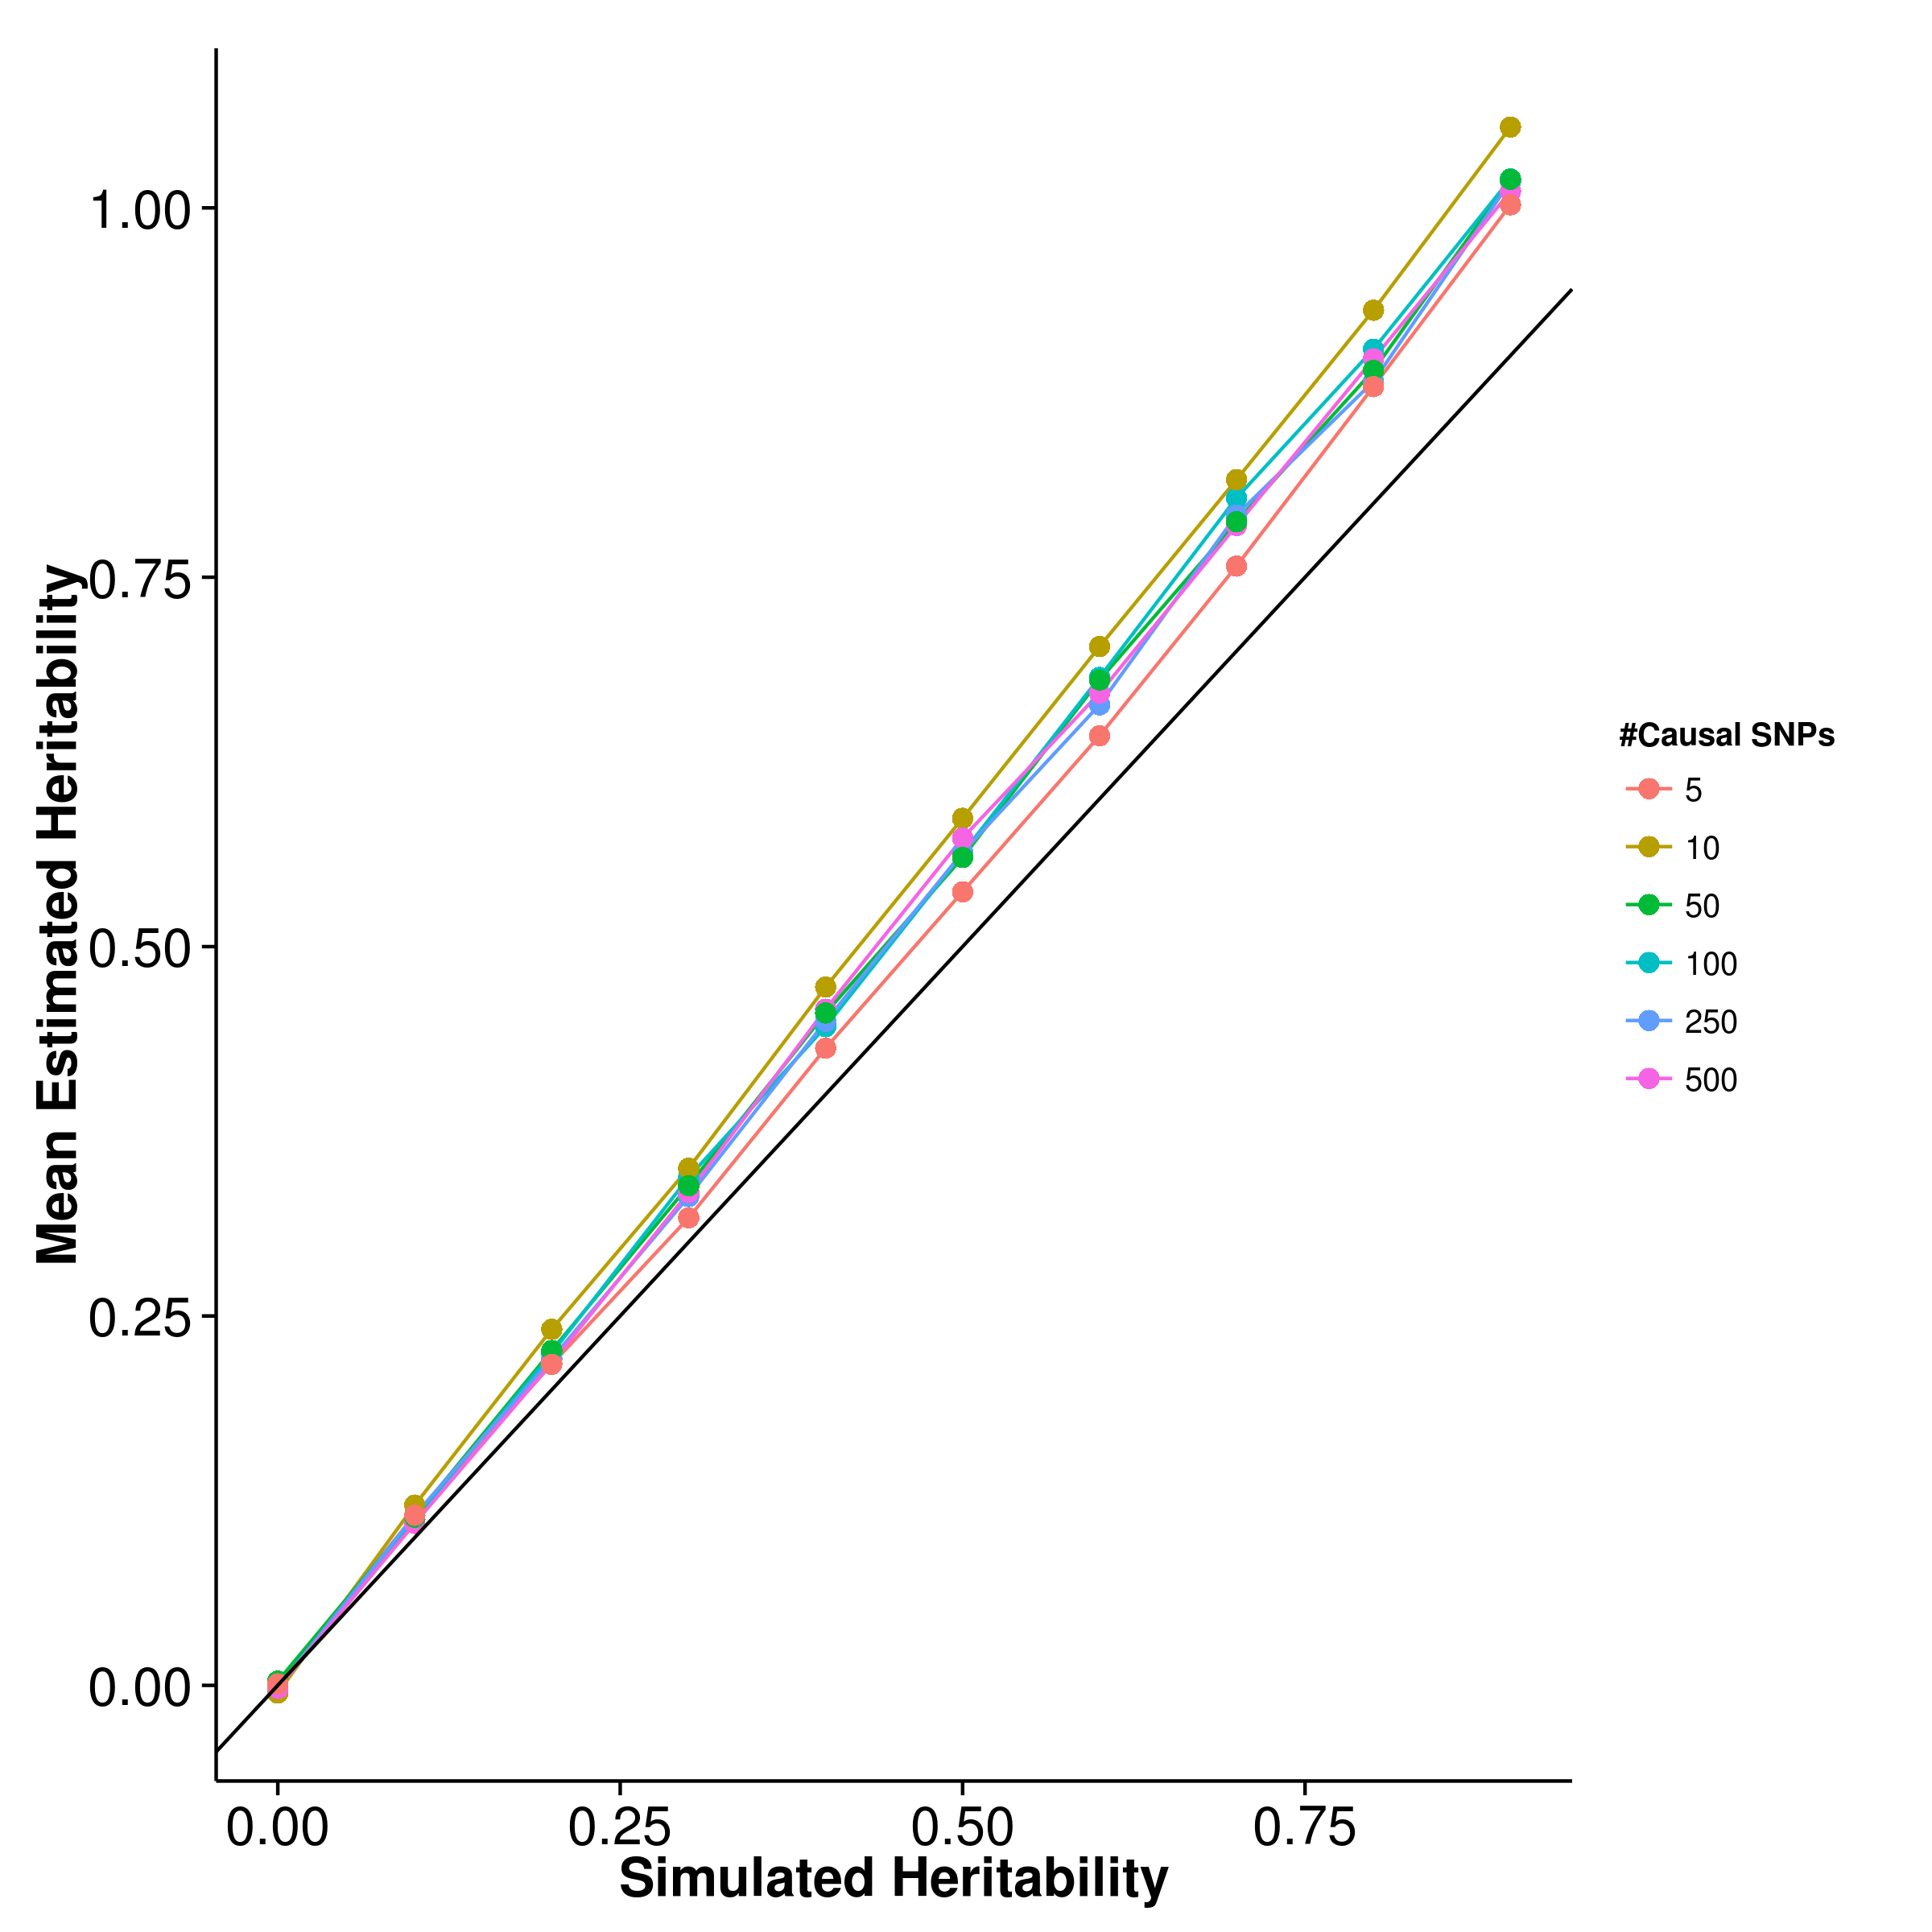
\includegraphics{figure/he_summary/equal/ldsc_Qt_Equal_mean.png}}
				\label{fig:ldscQtEqualMean}
			}
			\subfloat[LDSC with intercept estimation]{
				
				\scalebox{.4}{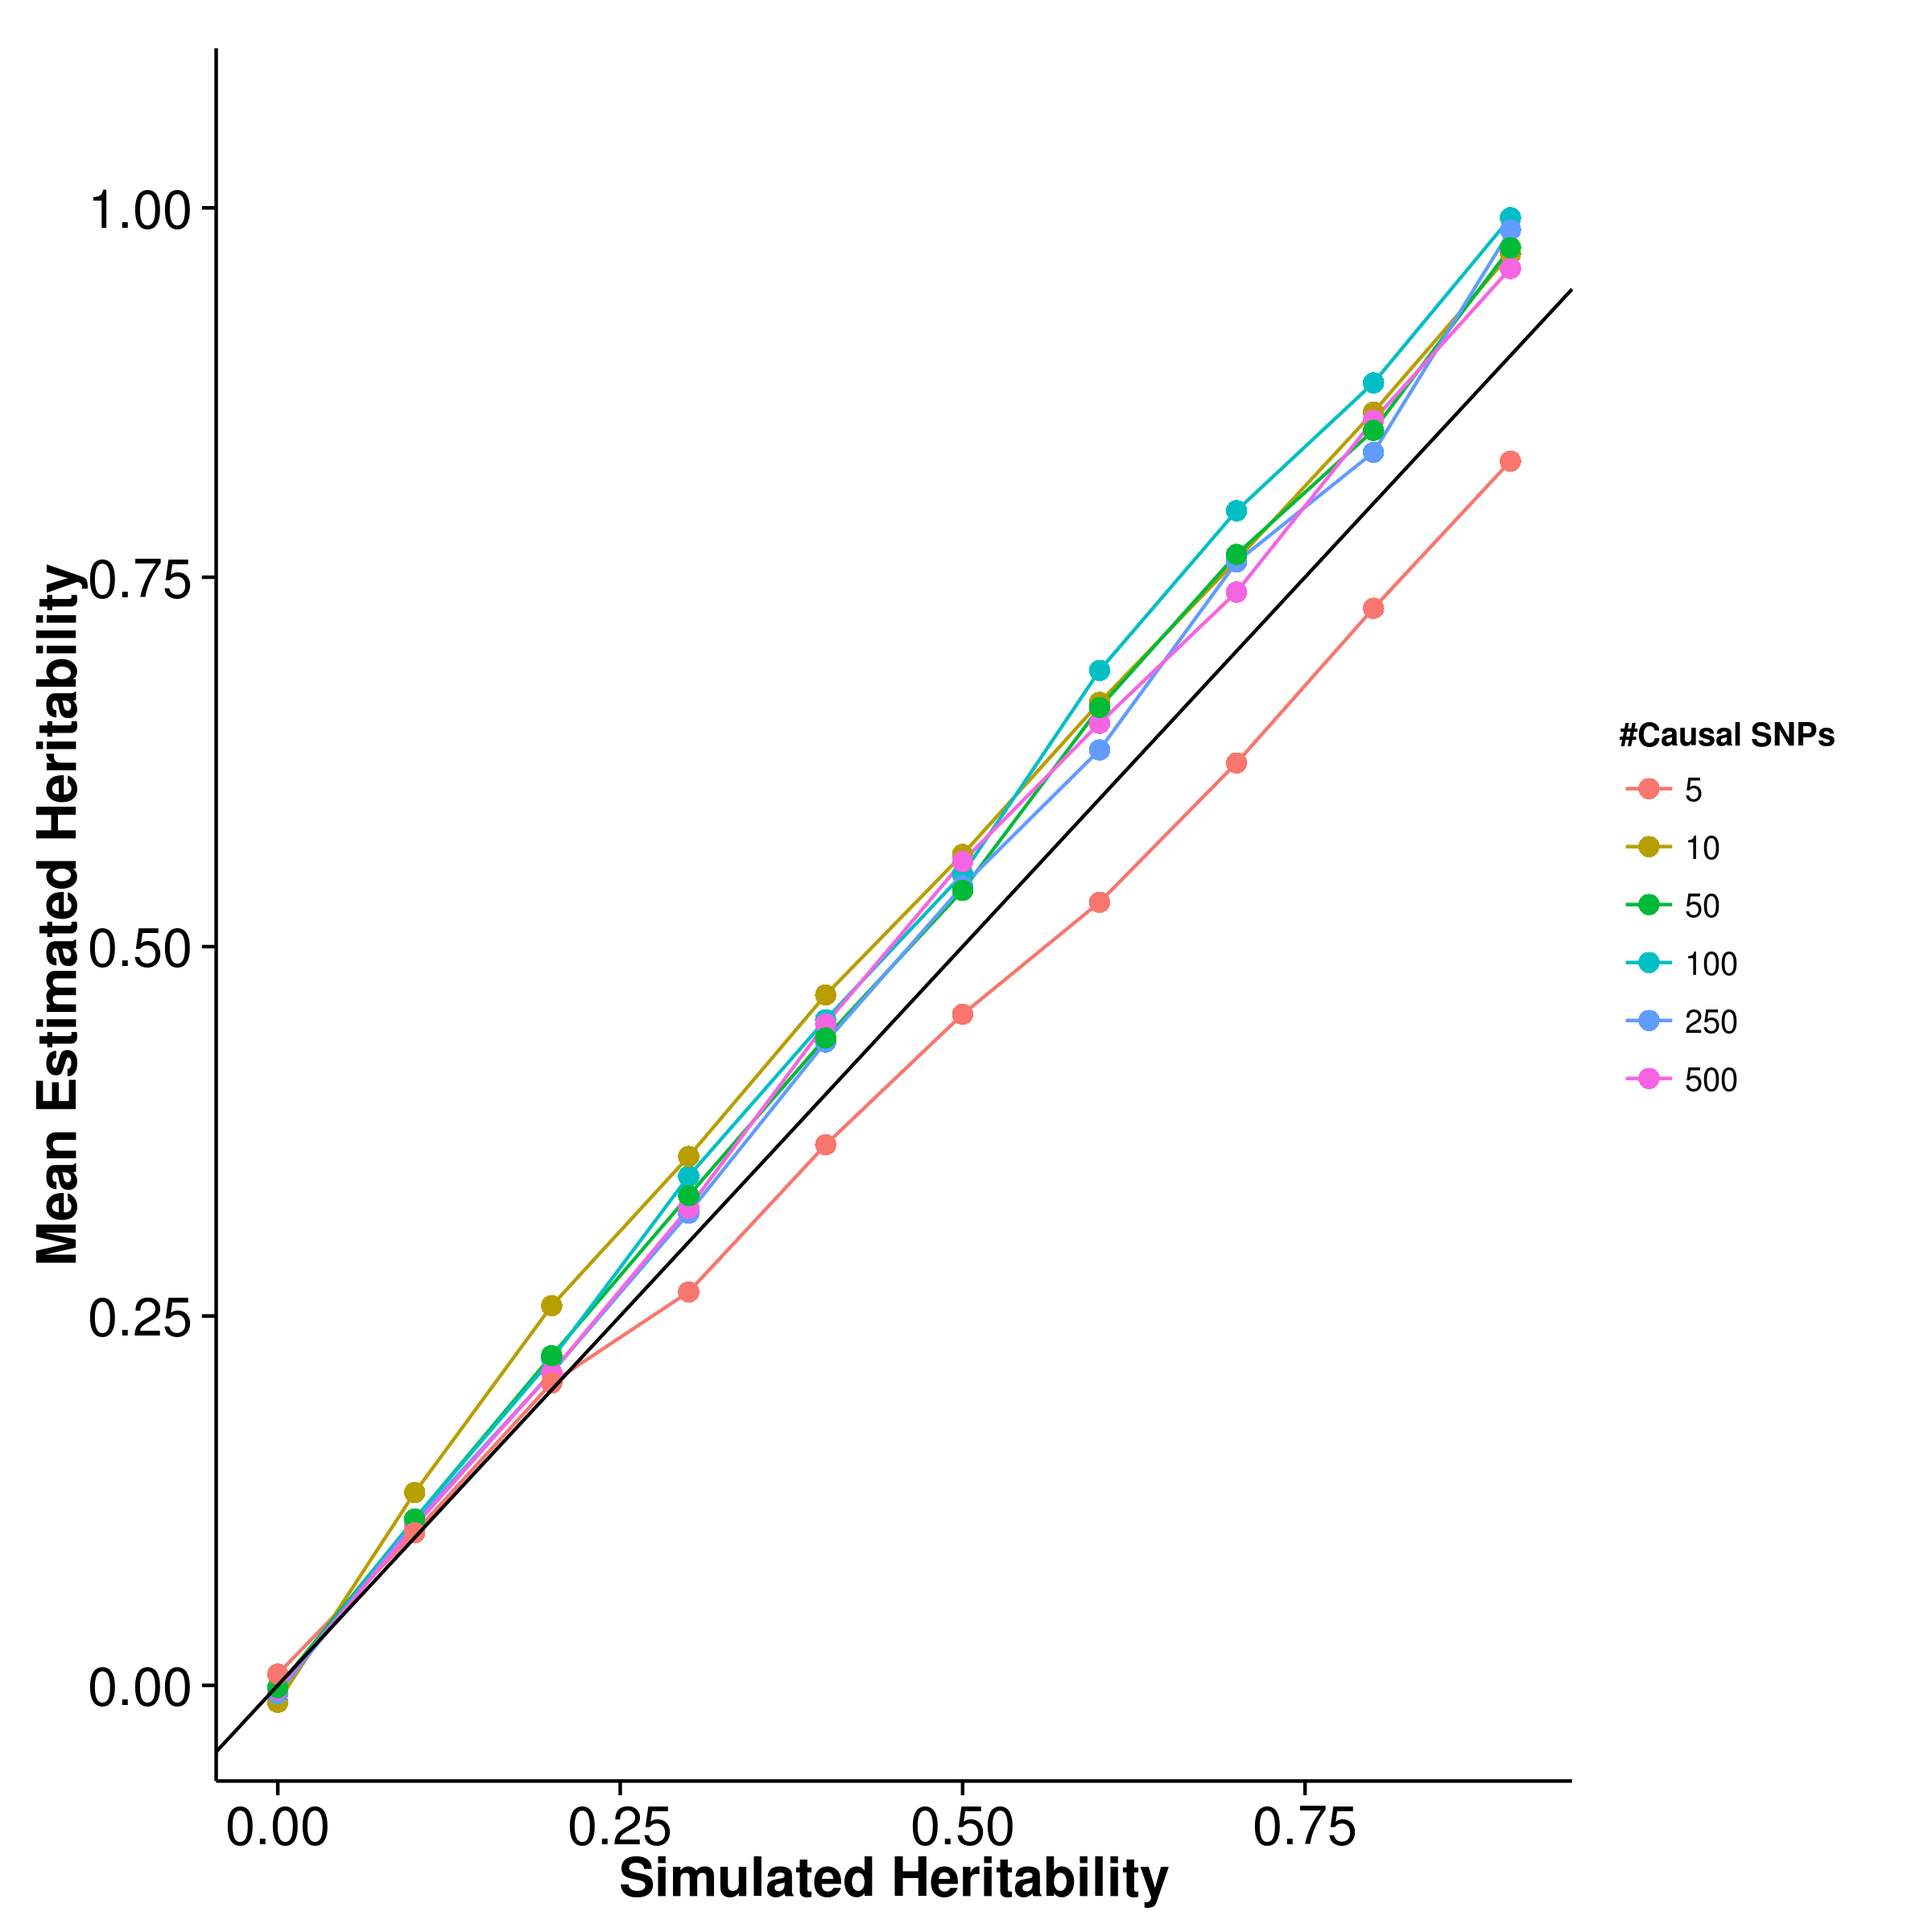
\includegraphics{figure/he_summary/equal/ldscIn_Qt_Equal_mean.png}}
				\label{fig:ldscInQtEqualMean}
			}
			\caption[Quantitative Trait with Equal Effect Size Simulation Result(Mean)]
			{Mean of results from quantitative trait simulation with equal effect size simulation.
				\gls{shrek} was found to be less biased of all the tools whereas there was a slight upward bias for \gls{ldsc} when the intercept was fixed, especially when the number of causal \glspl{SNP} was small.} 
			\label{fig:QtEqualMean}
		\end{figure}
		
		\begin{figure}
			\centering
			\subfloat[SHREK]{
				\scalebox{.4}{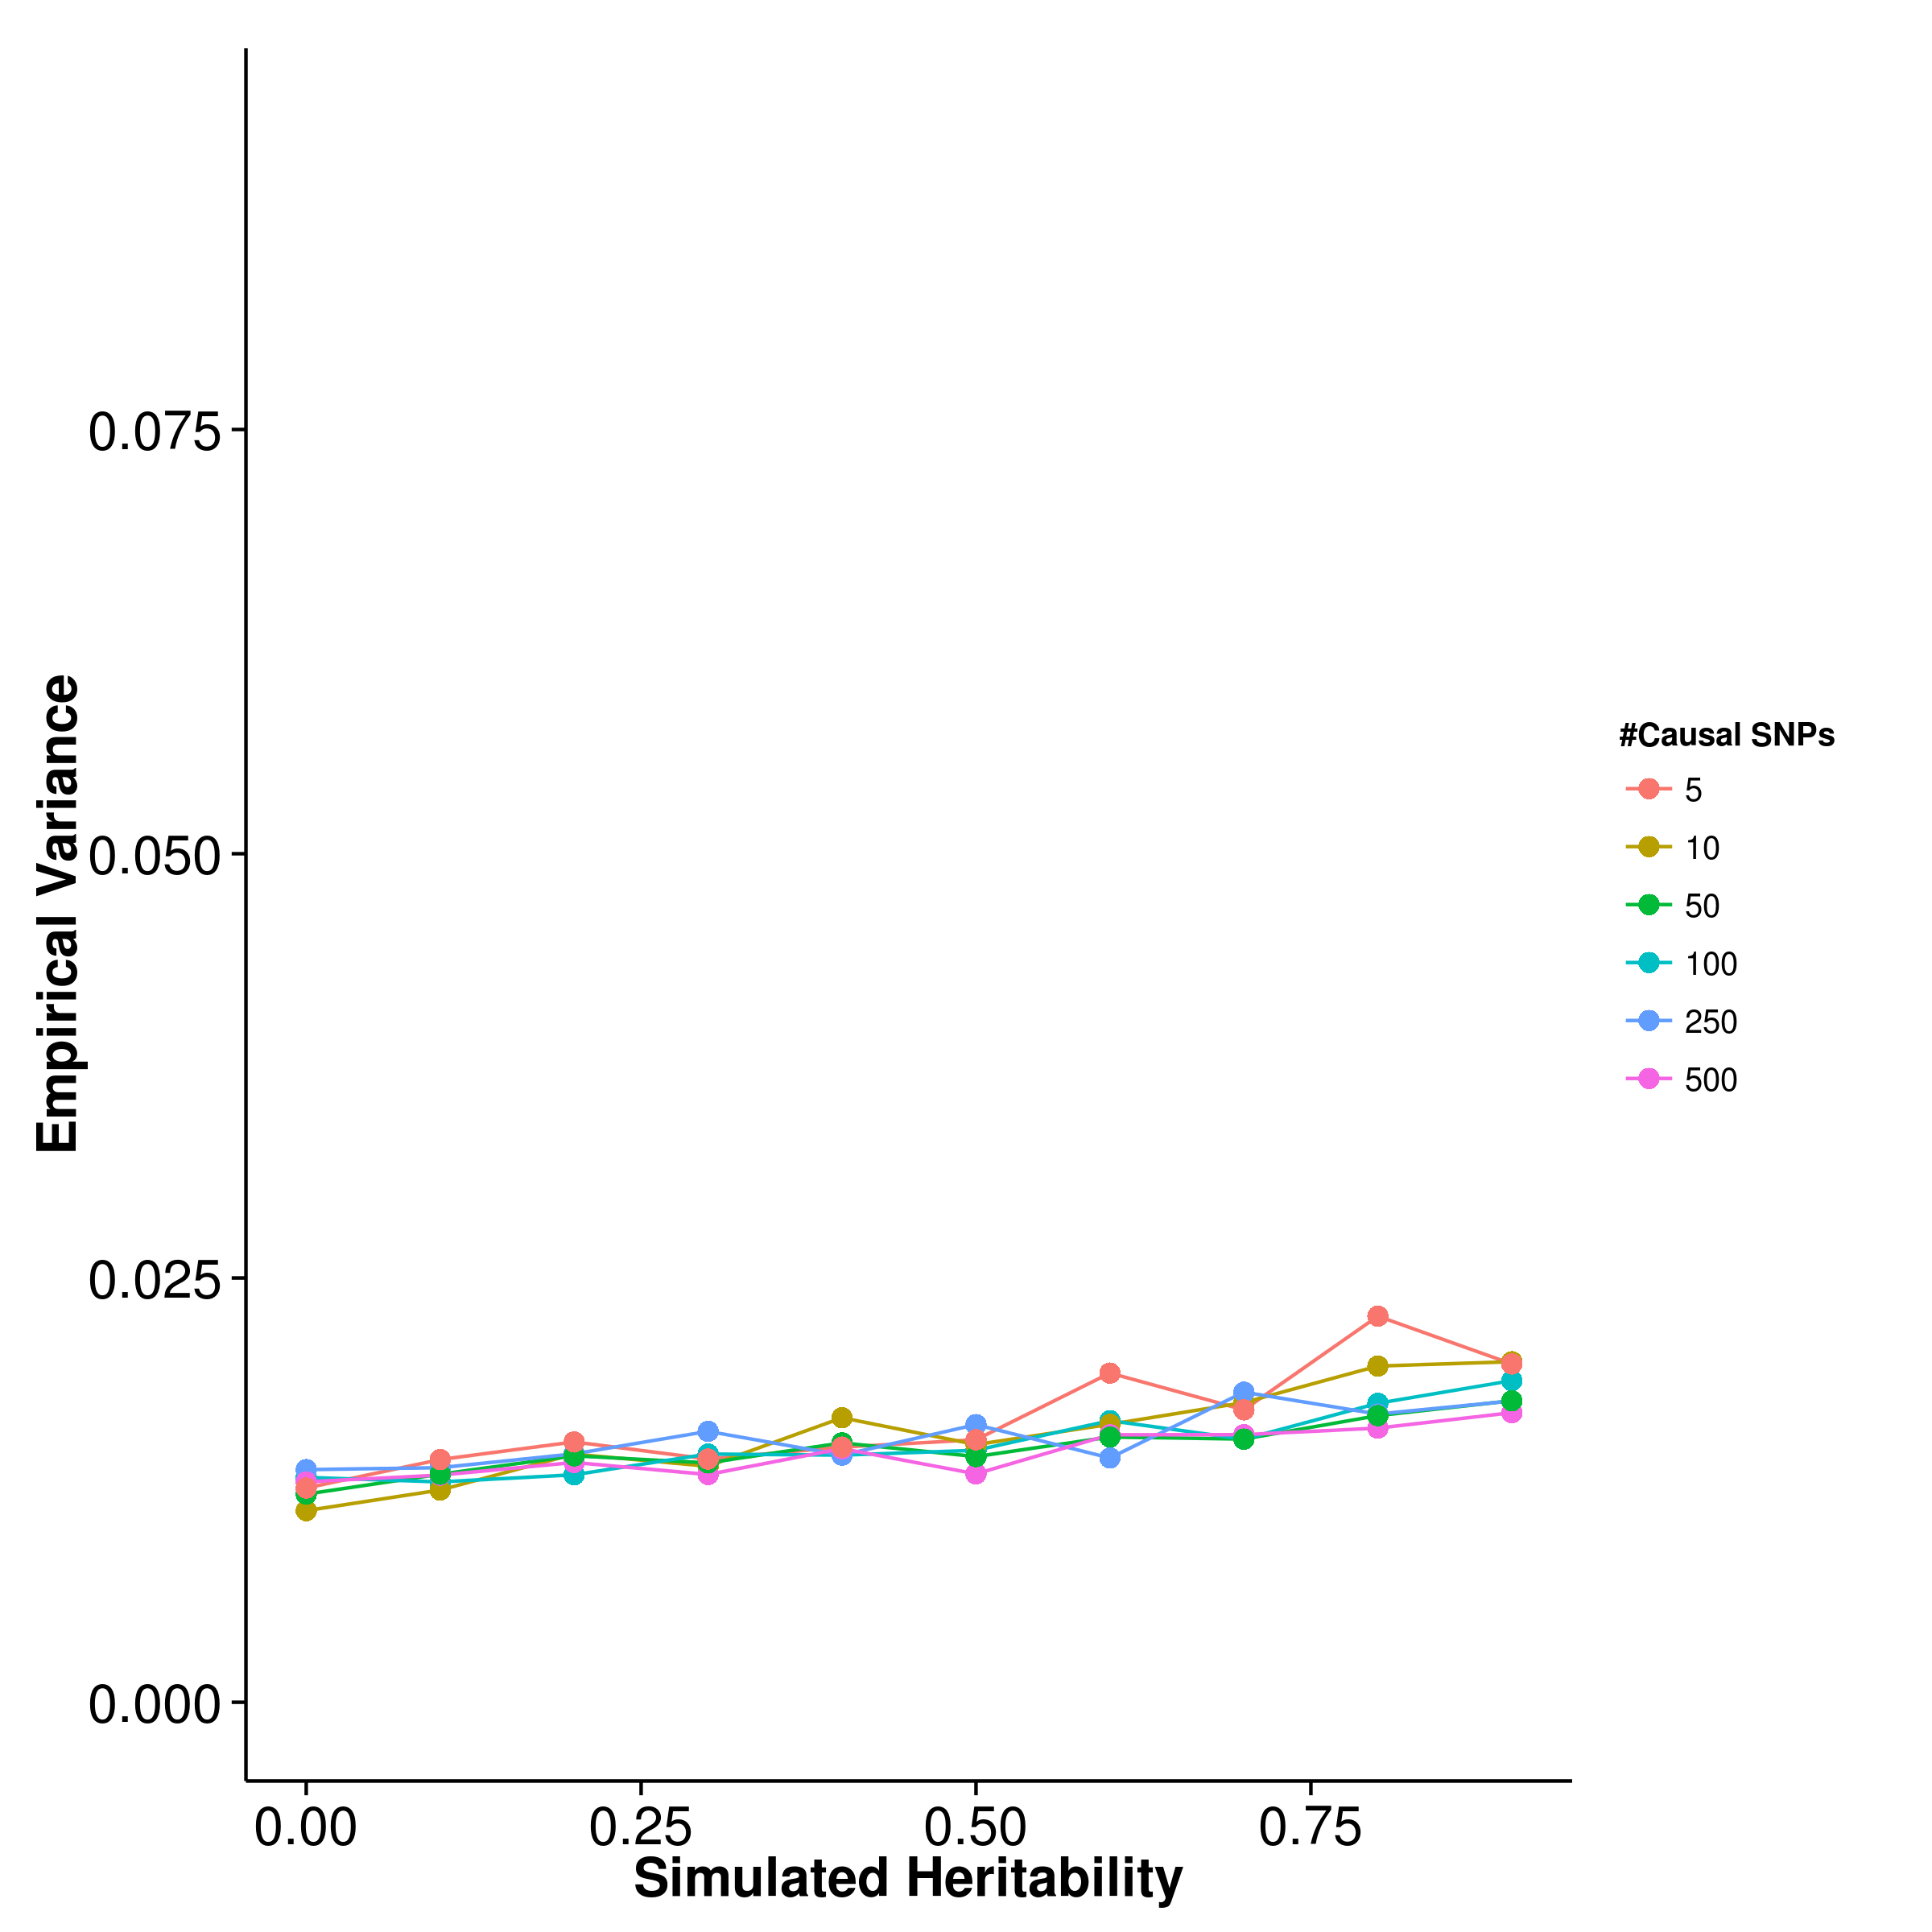
\includegraphics{figure/he_summary/equal/shrek_Qt_Equal_sd.png}}
				\label{fig:shrekQtEqualVar}
			}
			\subfloat[GCTA]{
				\scalebox{.4}{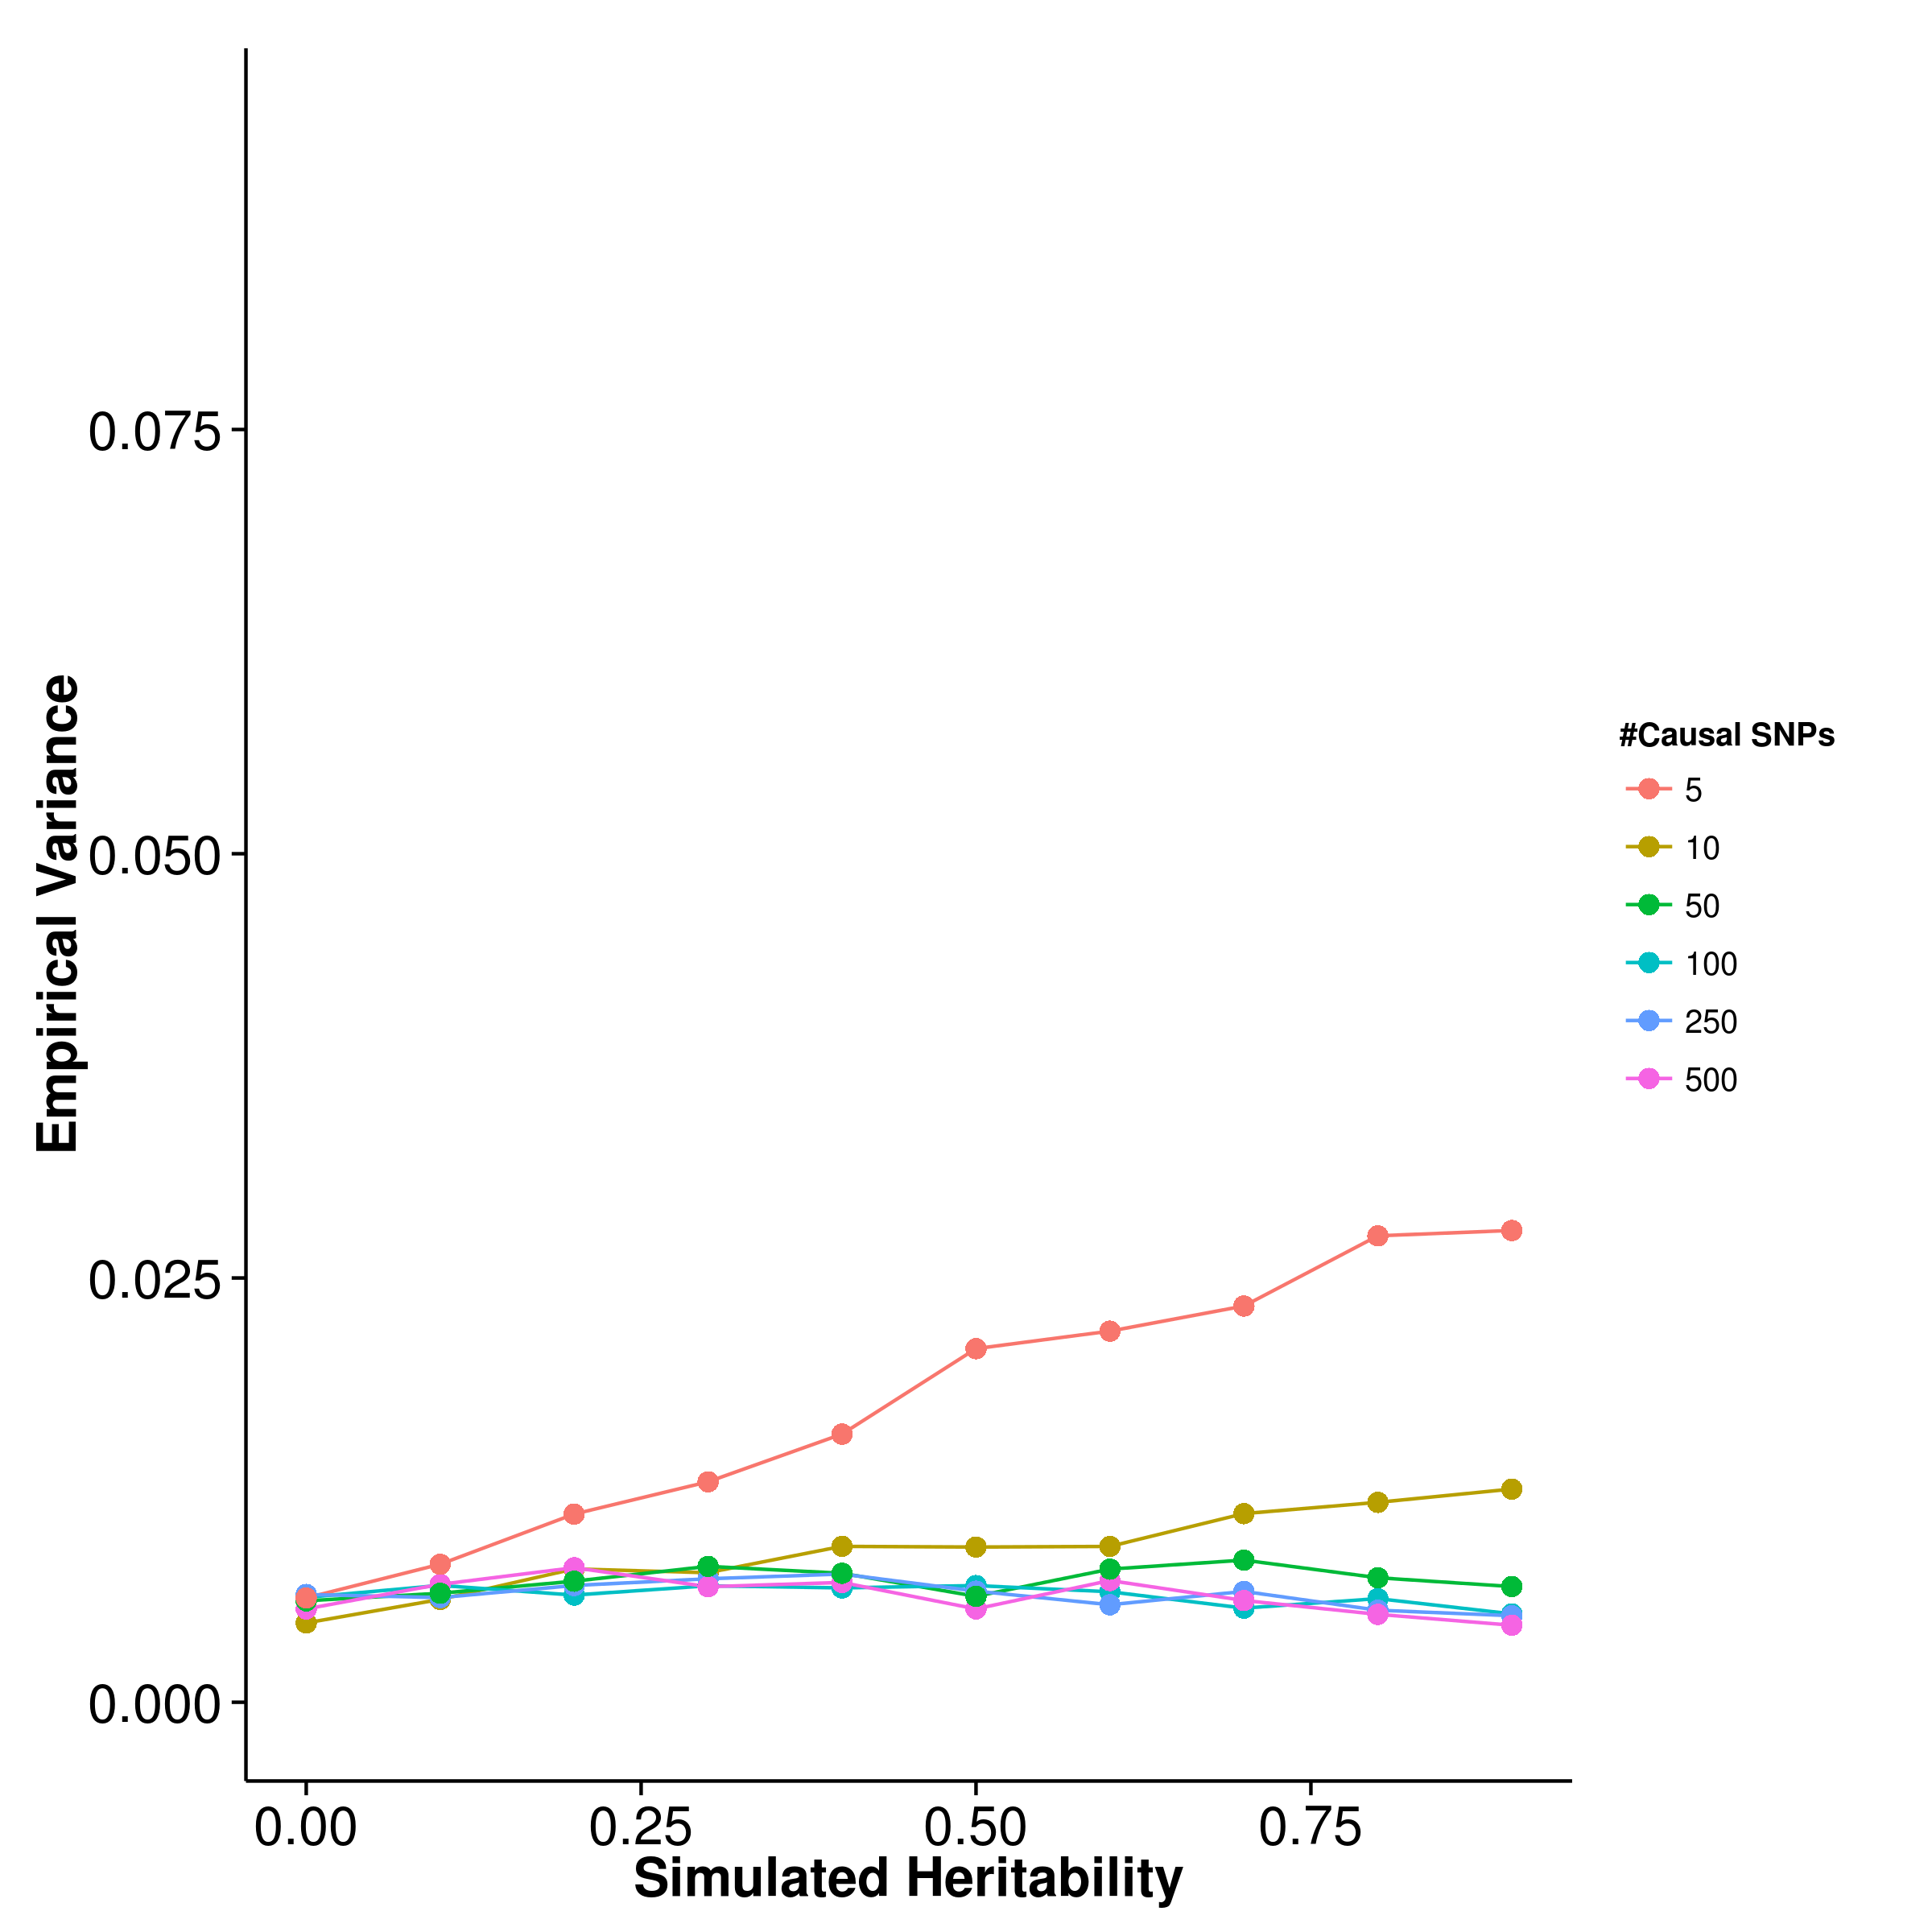
\includegraphics{figure/he_summary/equal/gcta_Qt_Equal_sd.png}}
				\label{fig:gctaQtEqualVar}
			}\\
			\subfloat[LDSC with fix intercept]{
				\scalebox{.4}{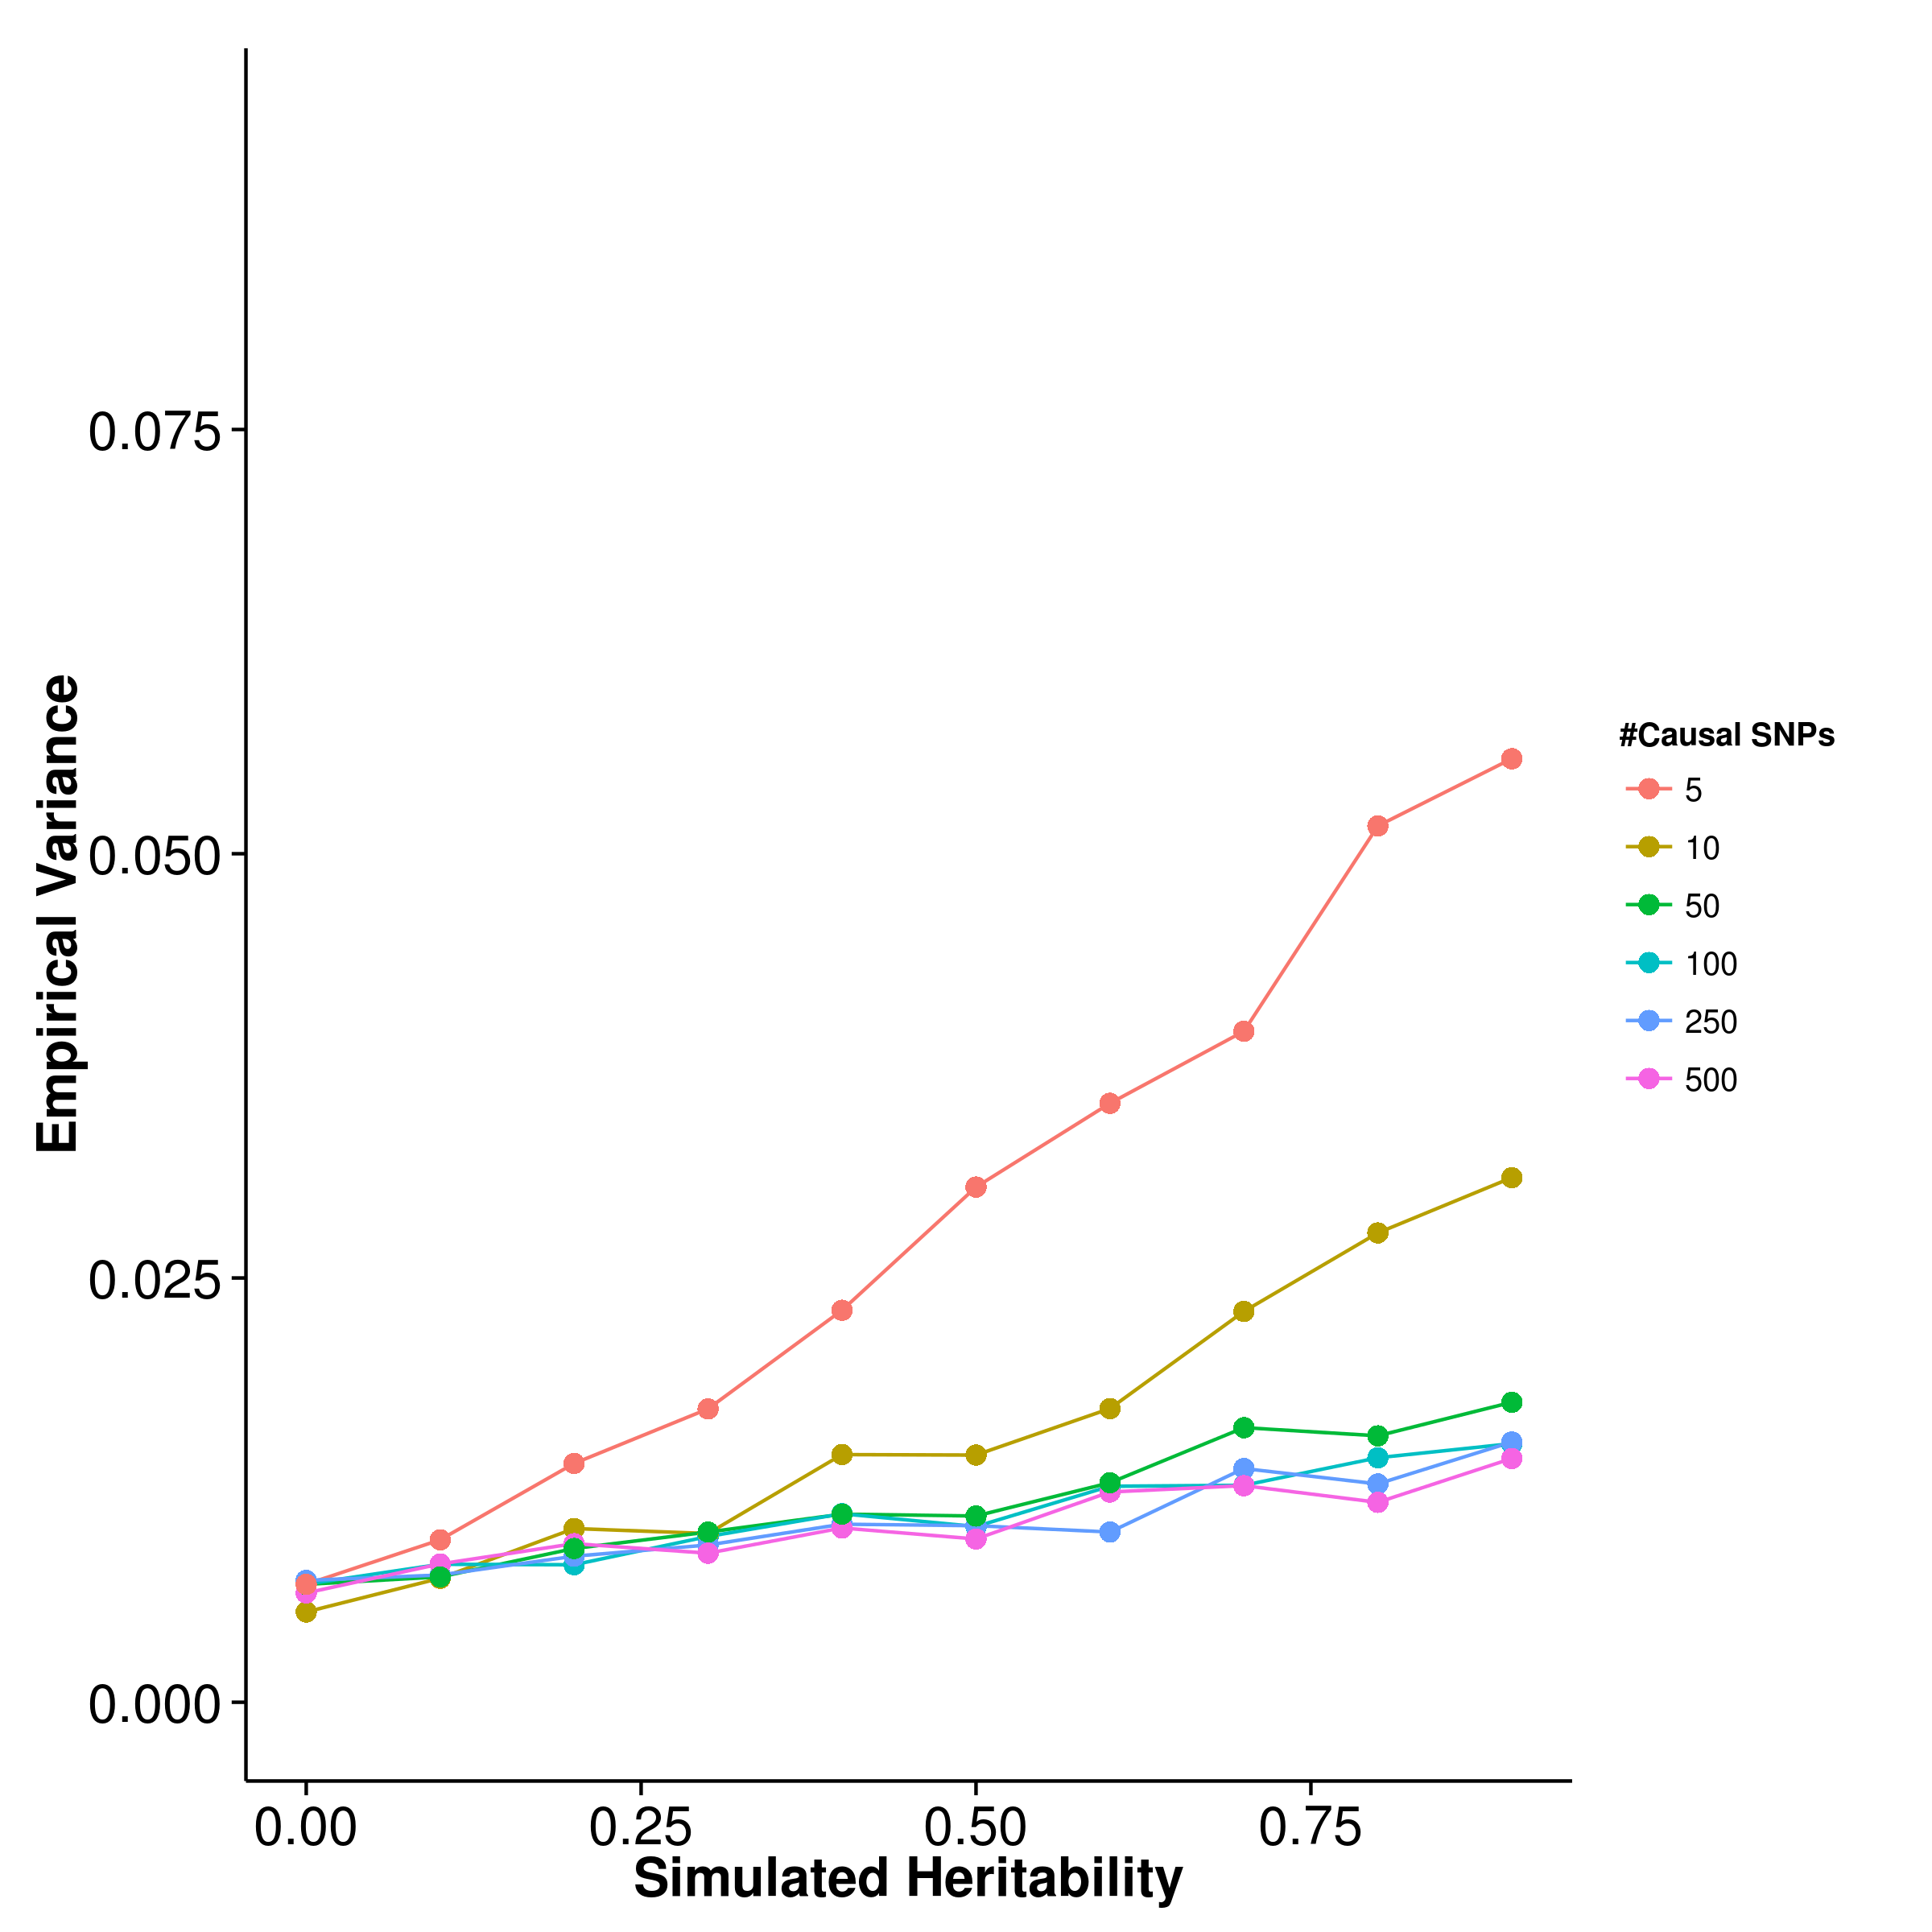
\includegraphics{figure/he_summary/equal/ldsc_Qt_Equal_sd.png}}
				\label{fig:ldscQtEqualVar}
			}
			\subfloat[LDSC with intercept estimation]{
				
				\scalebox{.4}{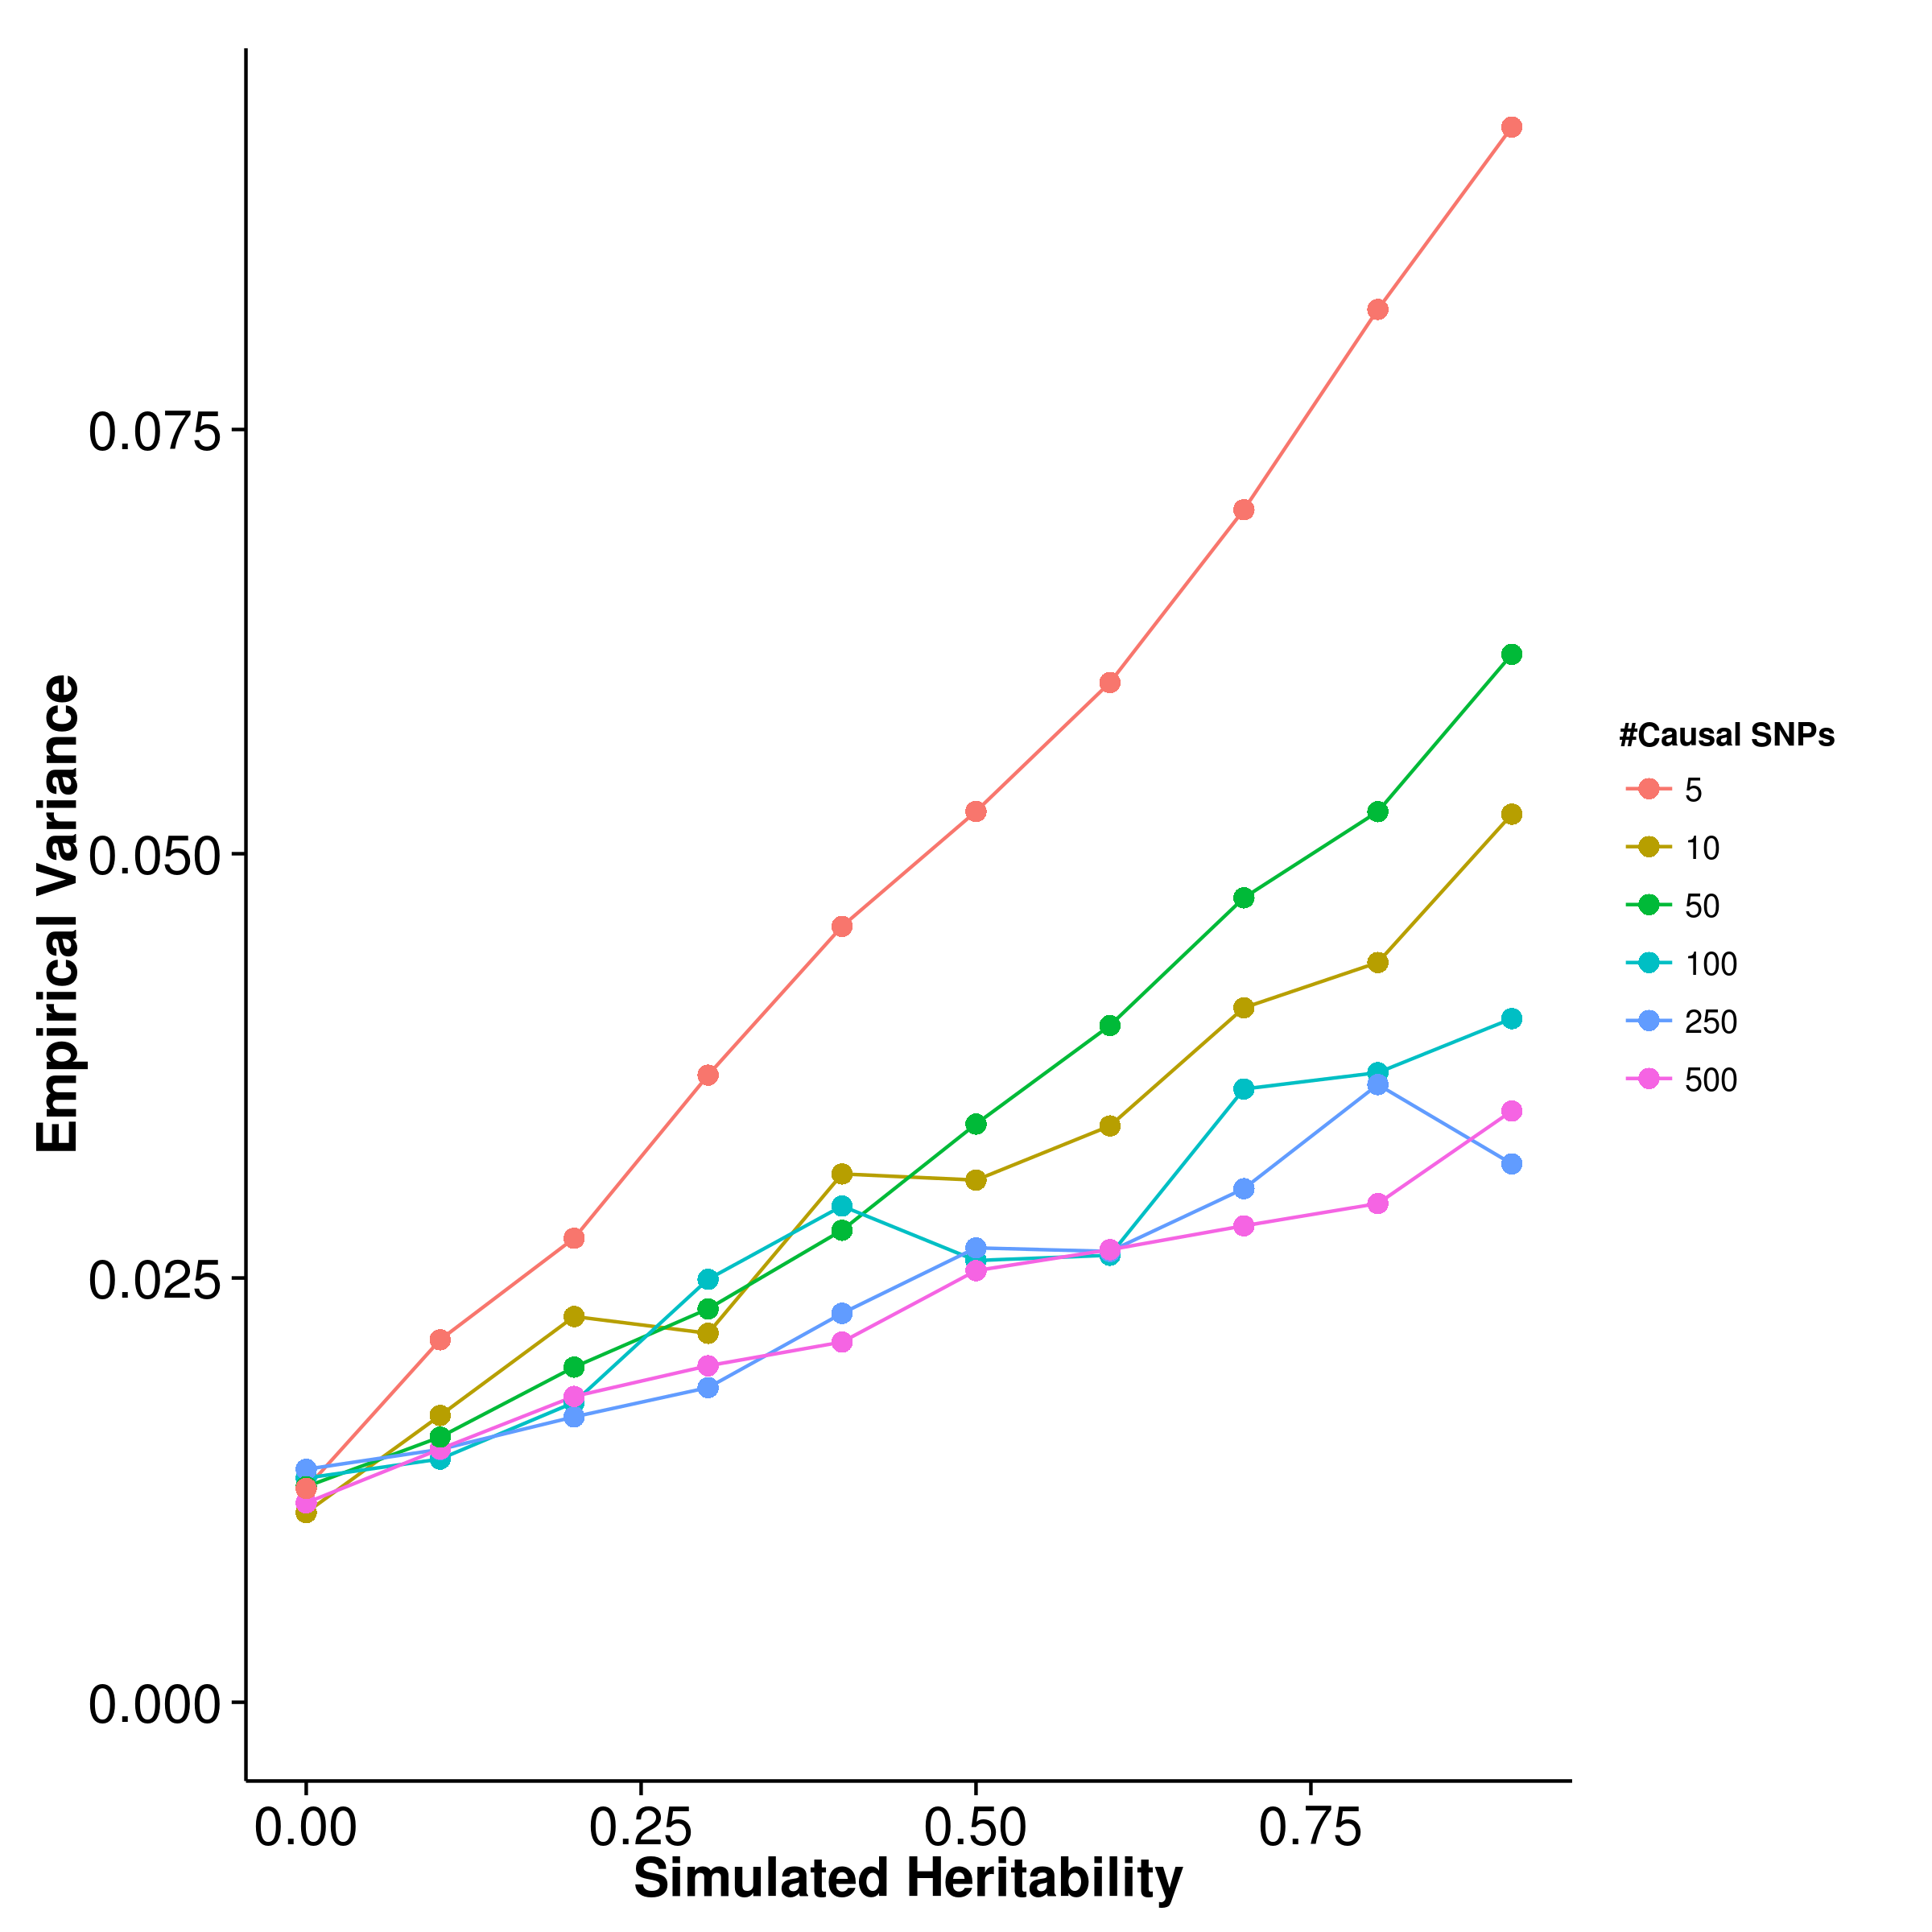
\includegraphics{figure/he_summary/equal/ldscIn_Qt_Equal_sd.png}}
				\label{fig:ldscInQtEqualVar}
			}
			\caption[Quantitative Trait with Equal Effect Size Simulation Result(Variance)]
			{Variance of results from quantitative trait simulation with equal effect size simulation.
				Of all the programmes, \gls{gcta} was found to have the lowest variance, follow by \gls{ldsc} with fixed intercept.
				The variance of \gls{shrek} was slightly higher than that of \gls{ldsc} with fixed intercept and is lower than that of \gls{ldsc} with intercept estimation.
				Unlike \gls{ldsc}, the variance of \gls{shrek} was less sensitive to change in total heritability.} 
			\label{fig:QtEqualVar}
		\end{figure}
		
		\begin{figure}
			\centering
			\subfloat[SHREK]{
				\scalebox{.4}{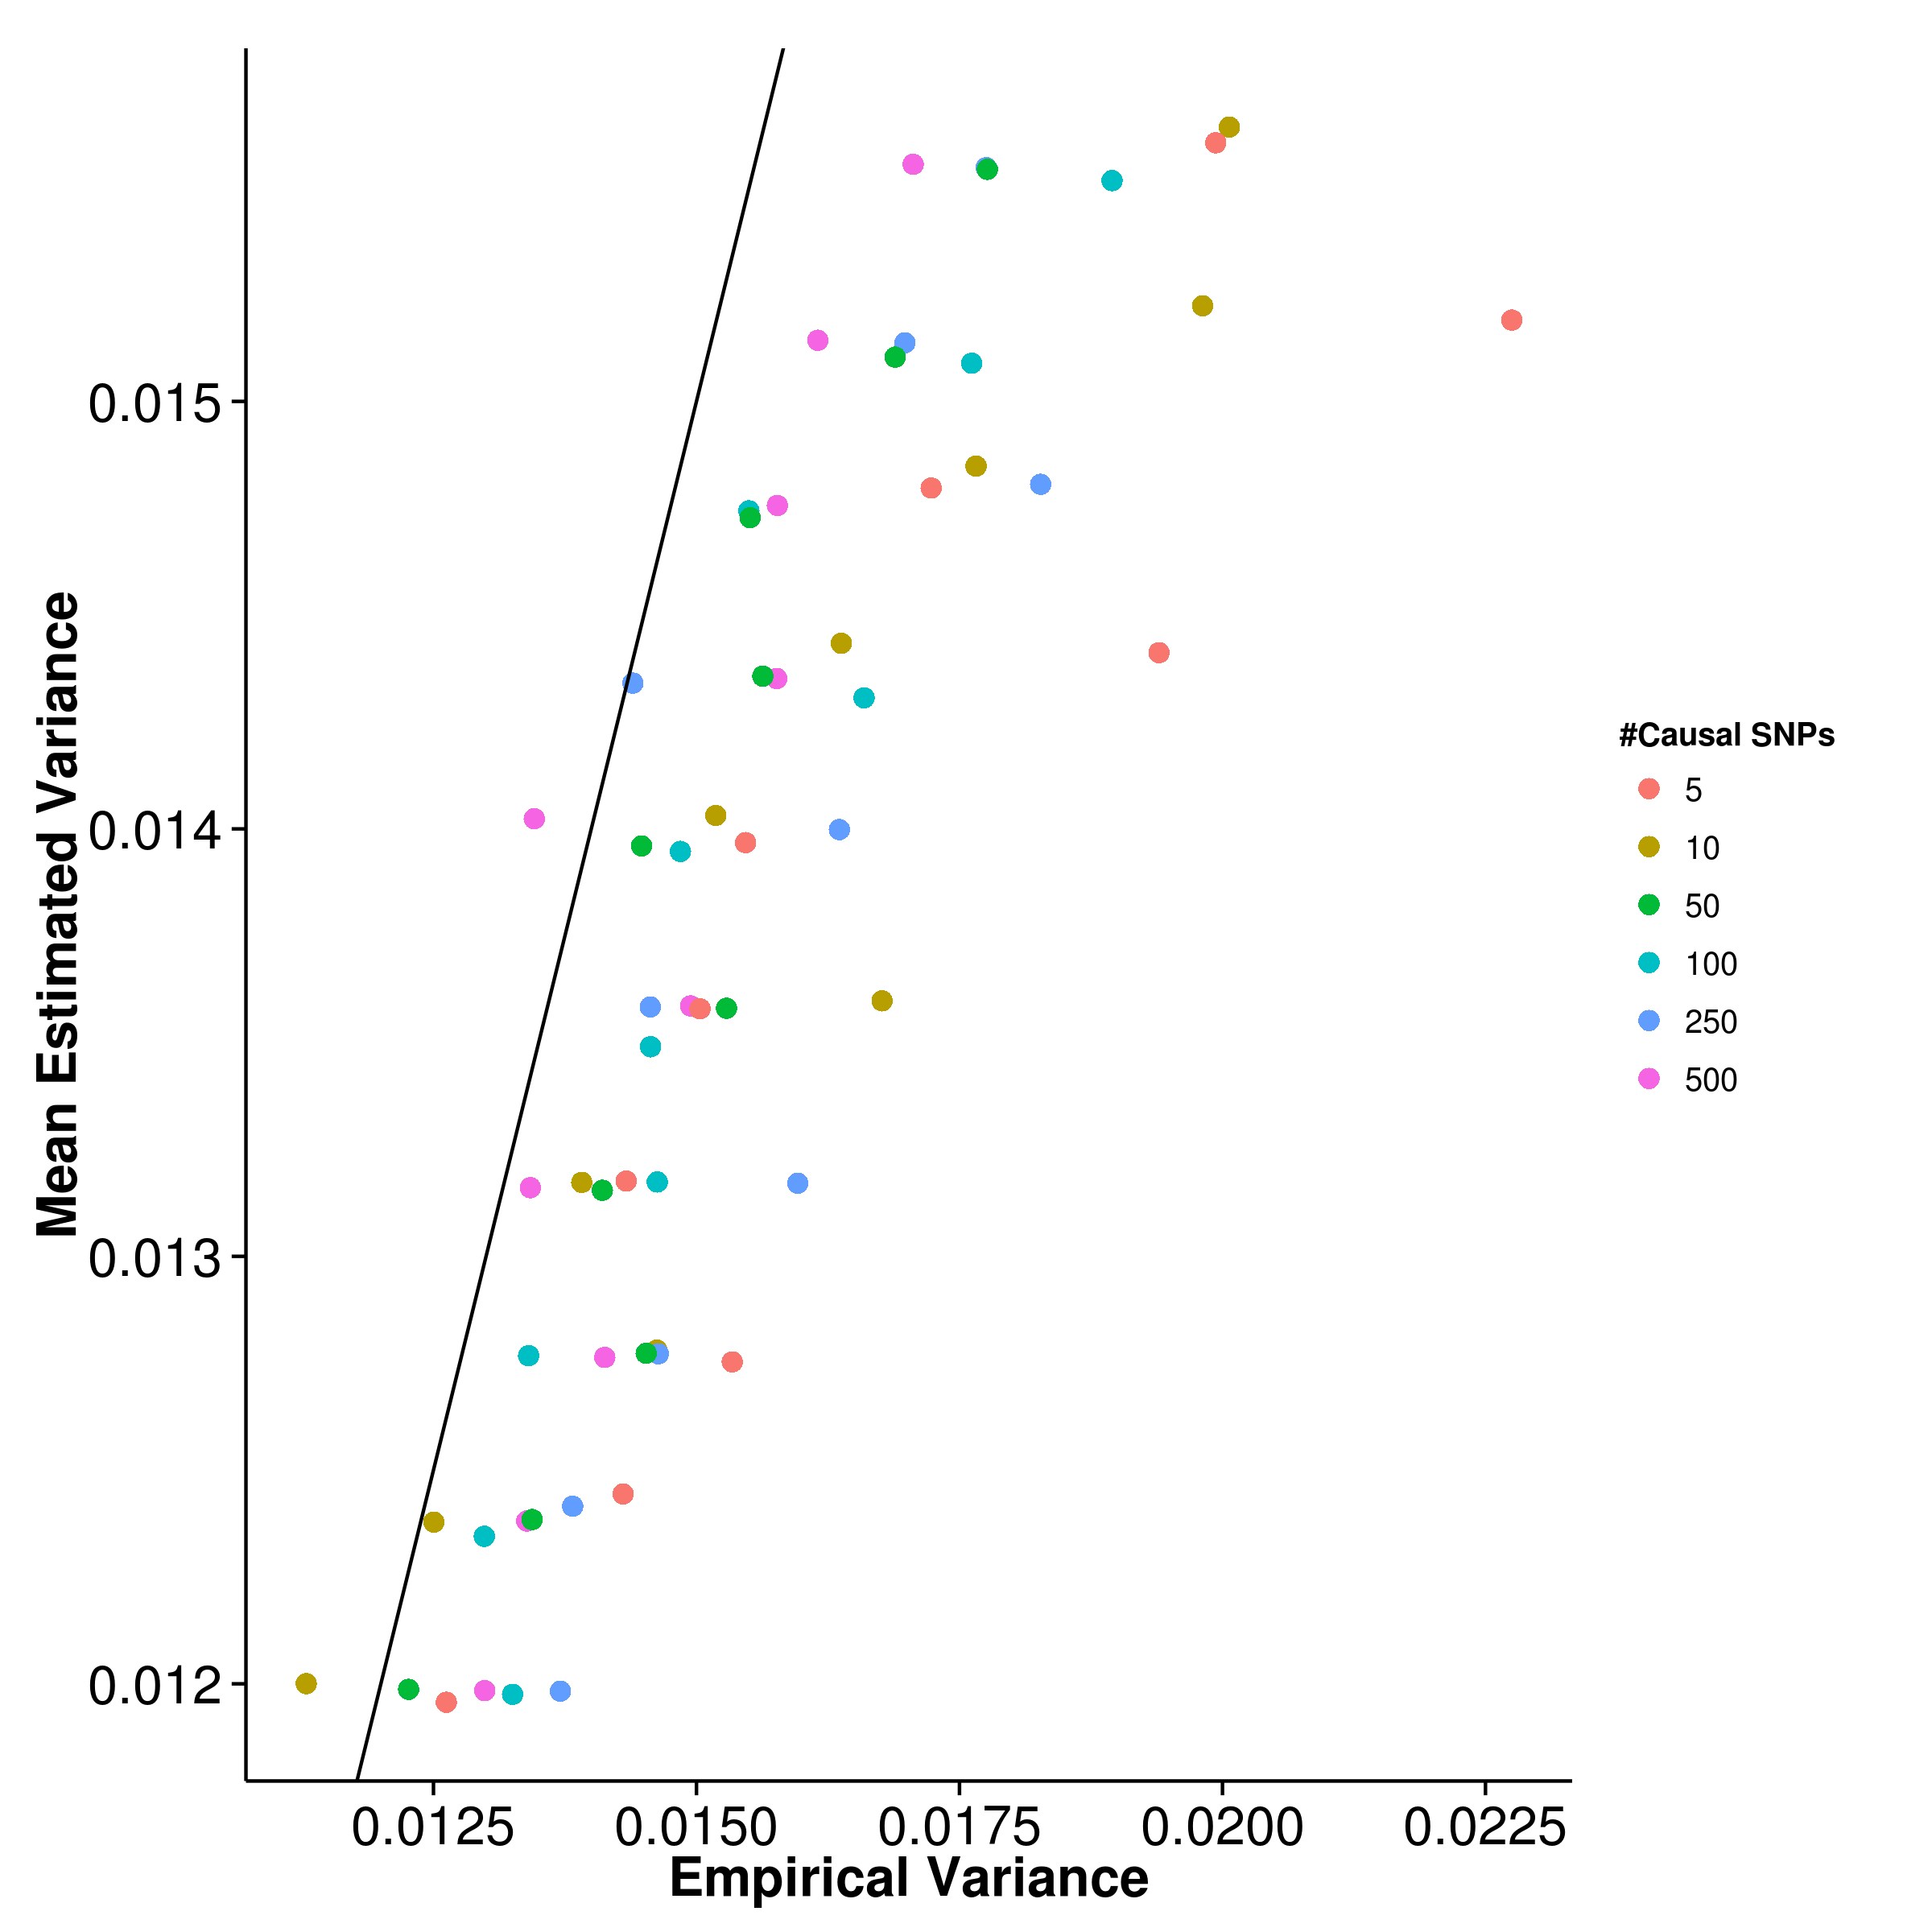
\includegraphics{figure/he_summary/equal/shrek_Qt_Equal_sdCom.png}}
				\label{fig:shrekQtEqualVarCom}
			}
			\subfloat[GCTA]{
				\scalebox{.4}{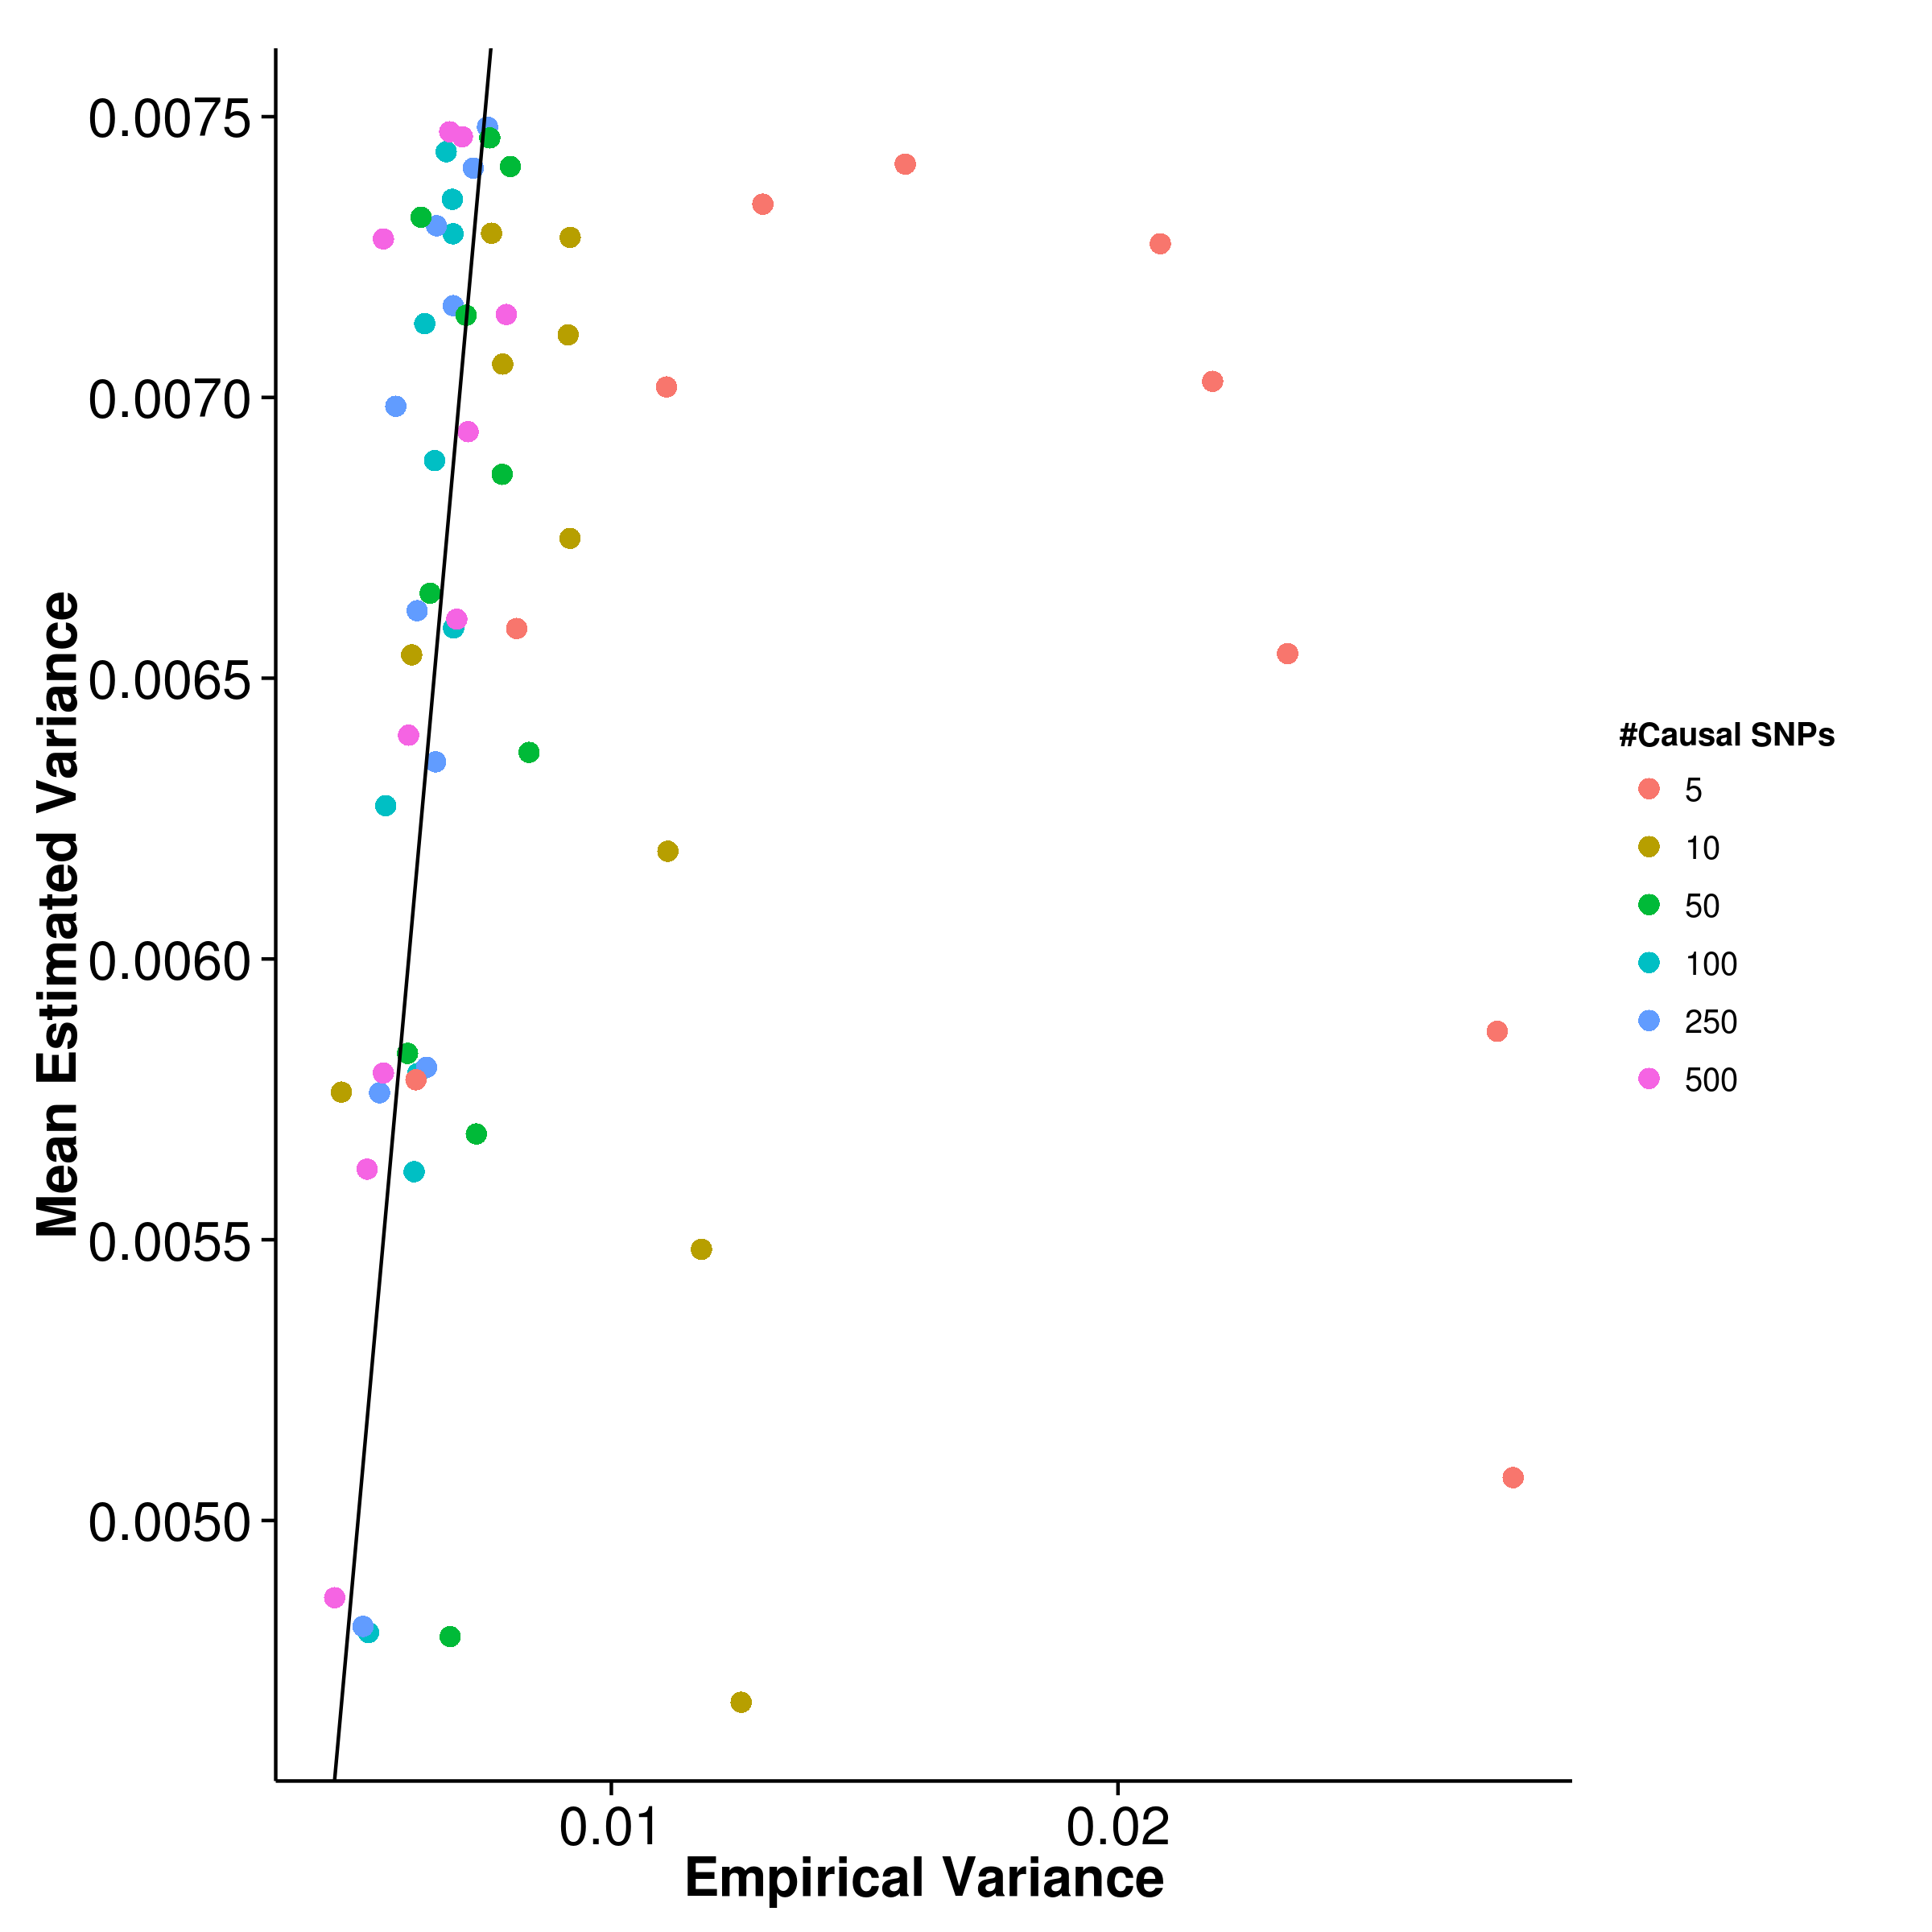
\includegraphics{figure/he_summary/equal/gcta_Qt_Equal_sdCom.png}}
				\label{fig:gctaQtEqualVarCom}
			}\\
			\subfloat[LDSC with fix intercept]{
				\scalebox{.4}{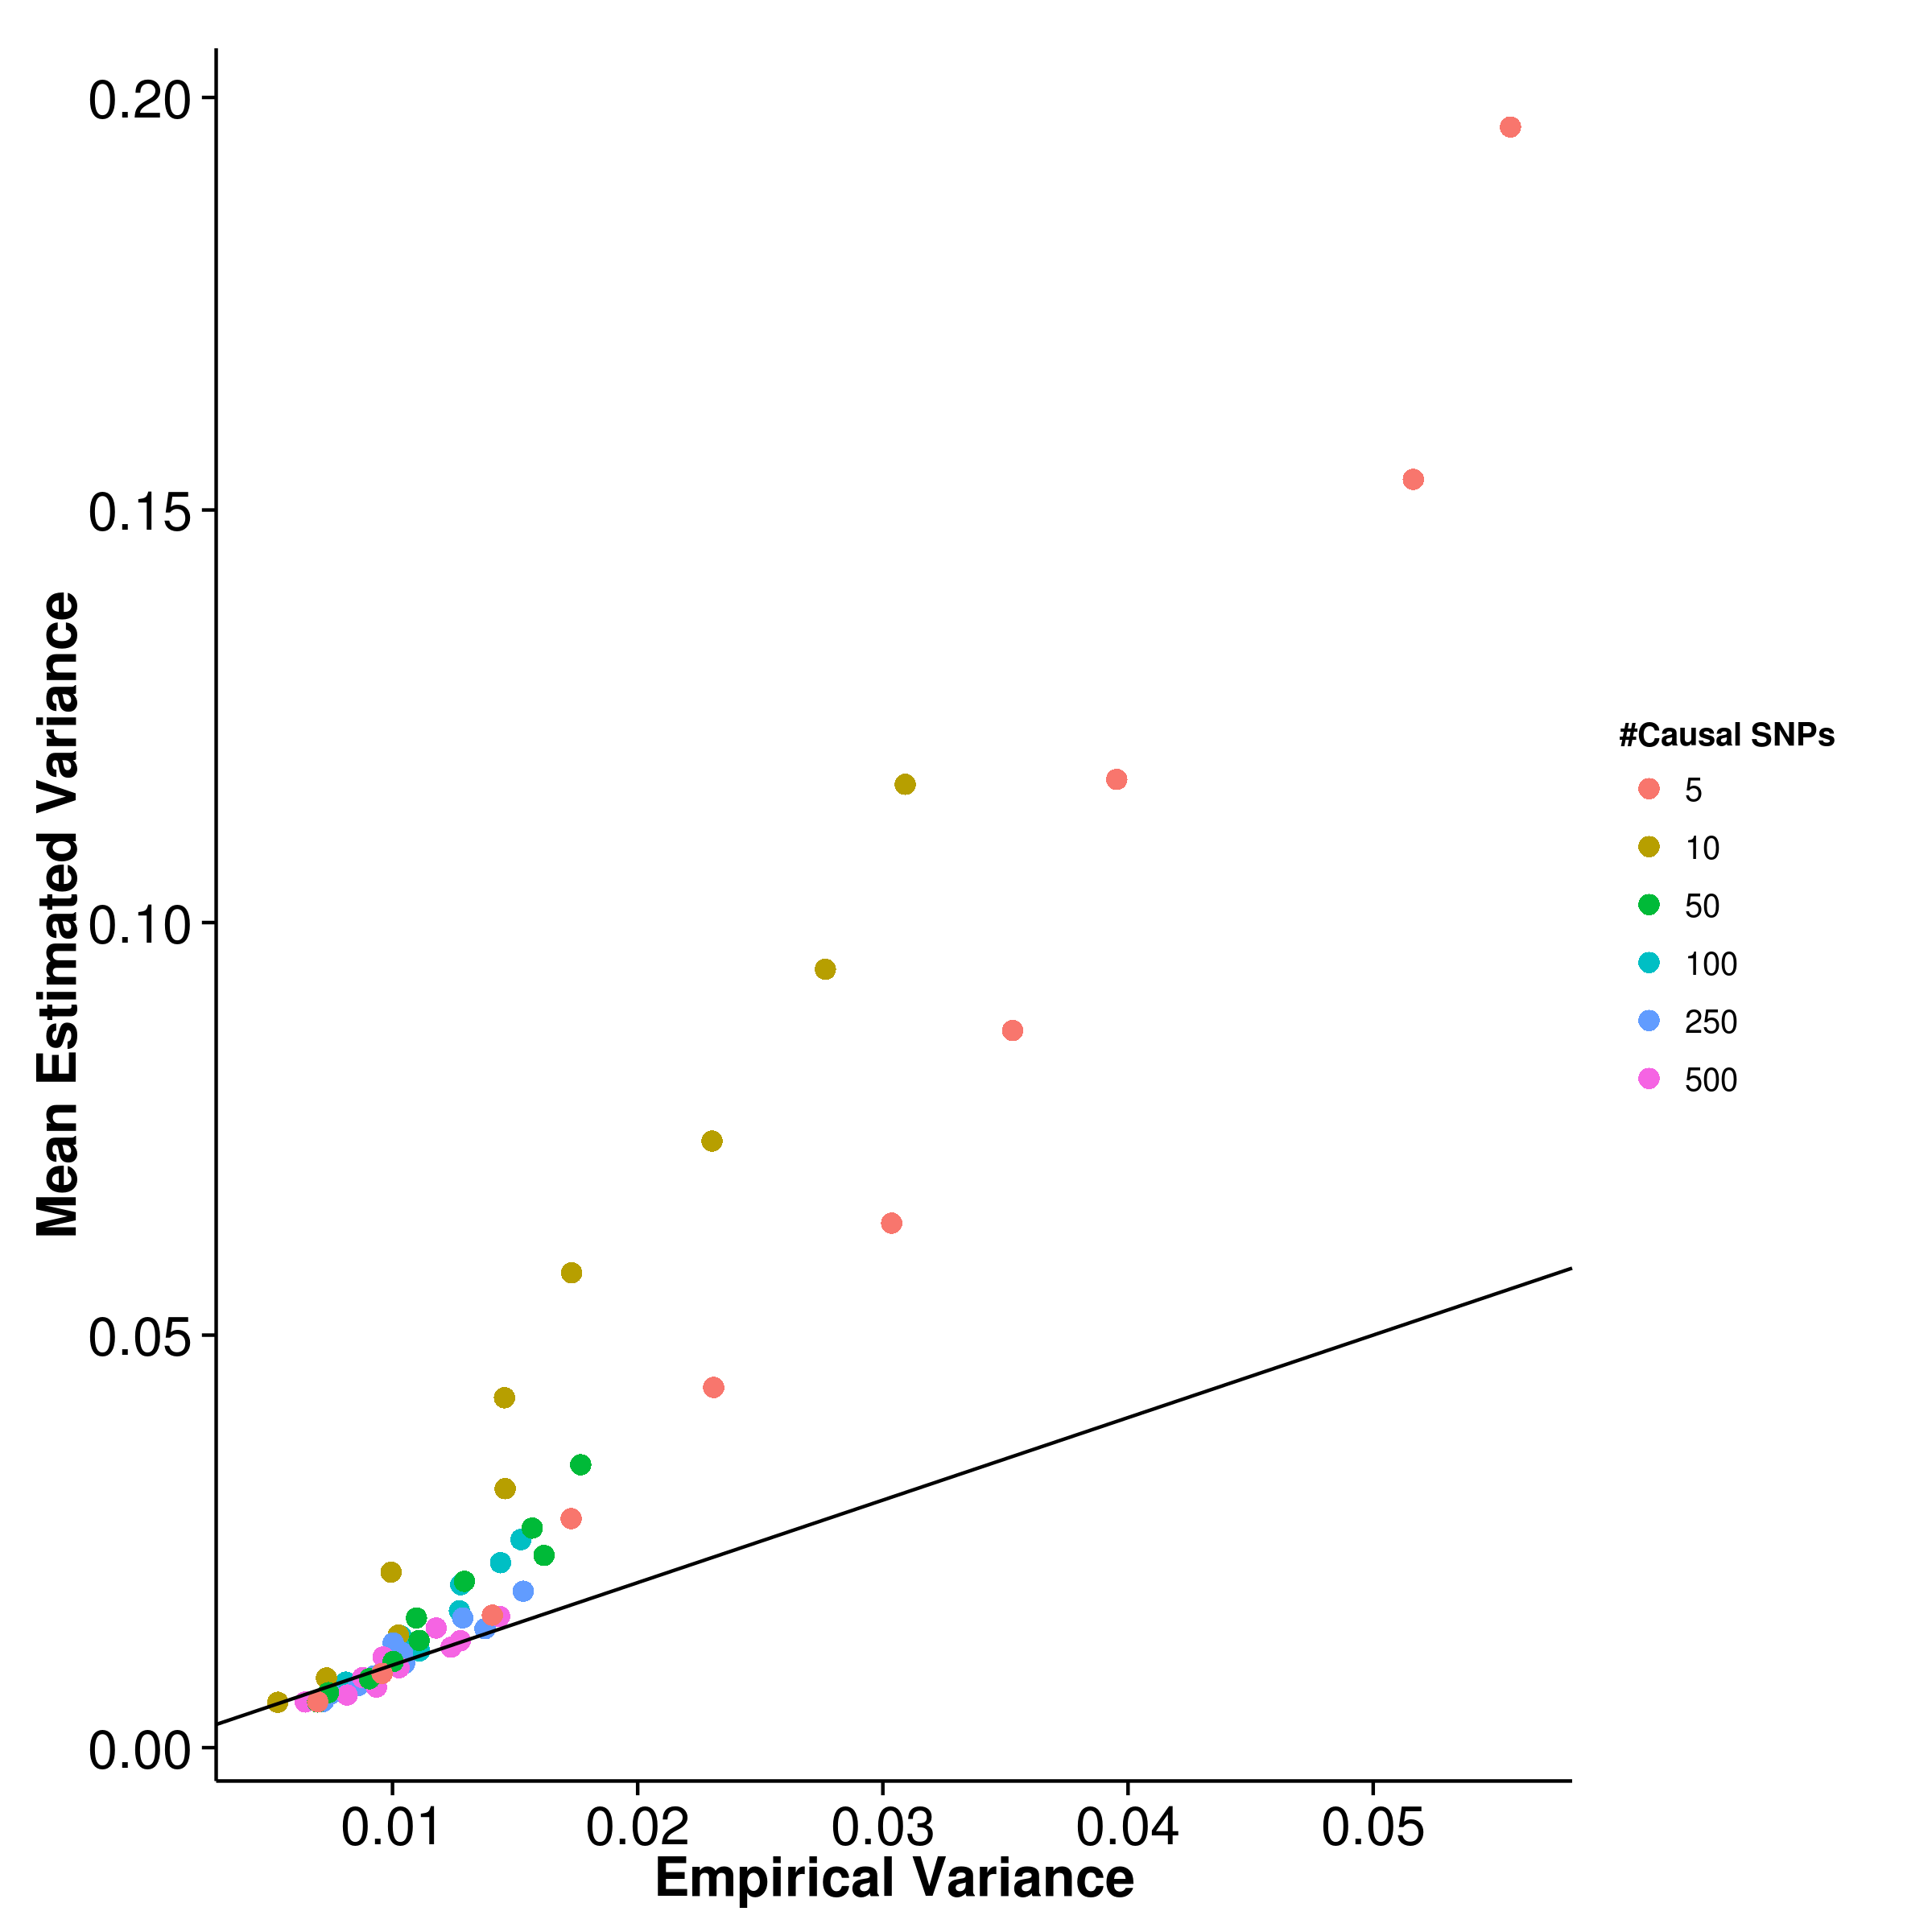
\includegraphics{figure/he_summary/equal/ldsc_Qt_Equal_sdCom.png}}
				\label{fig:ldscQtEqualVarCom}
			}
			\subfloat[LDSC with intercept estimation]{
				
				\scalebox{.4}{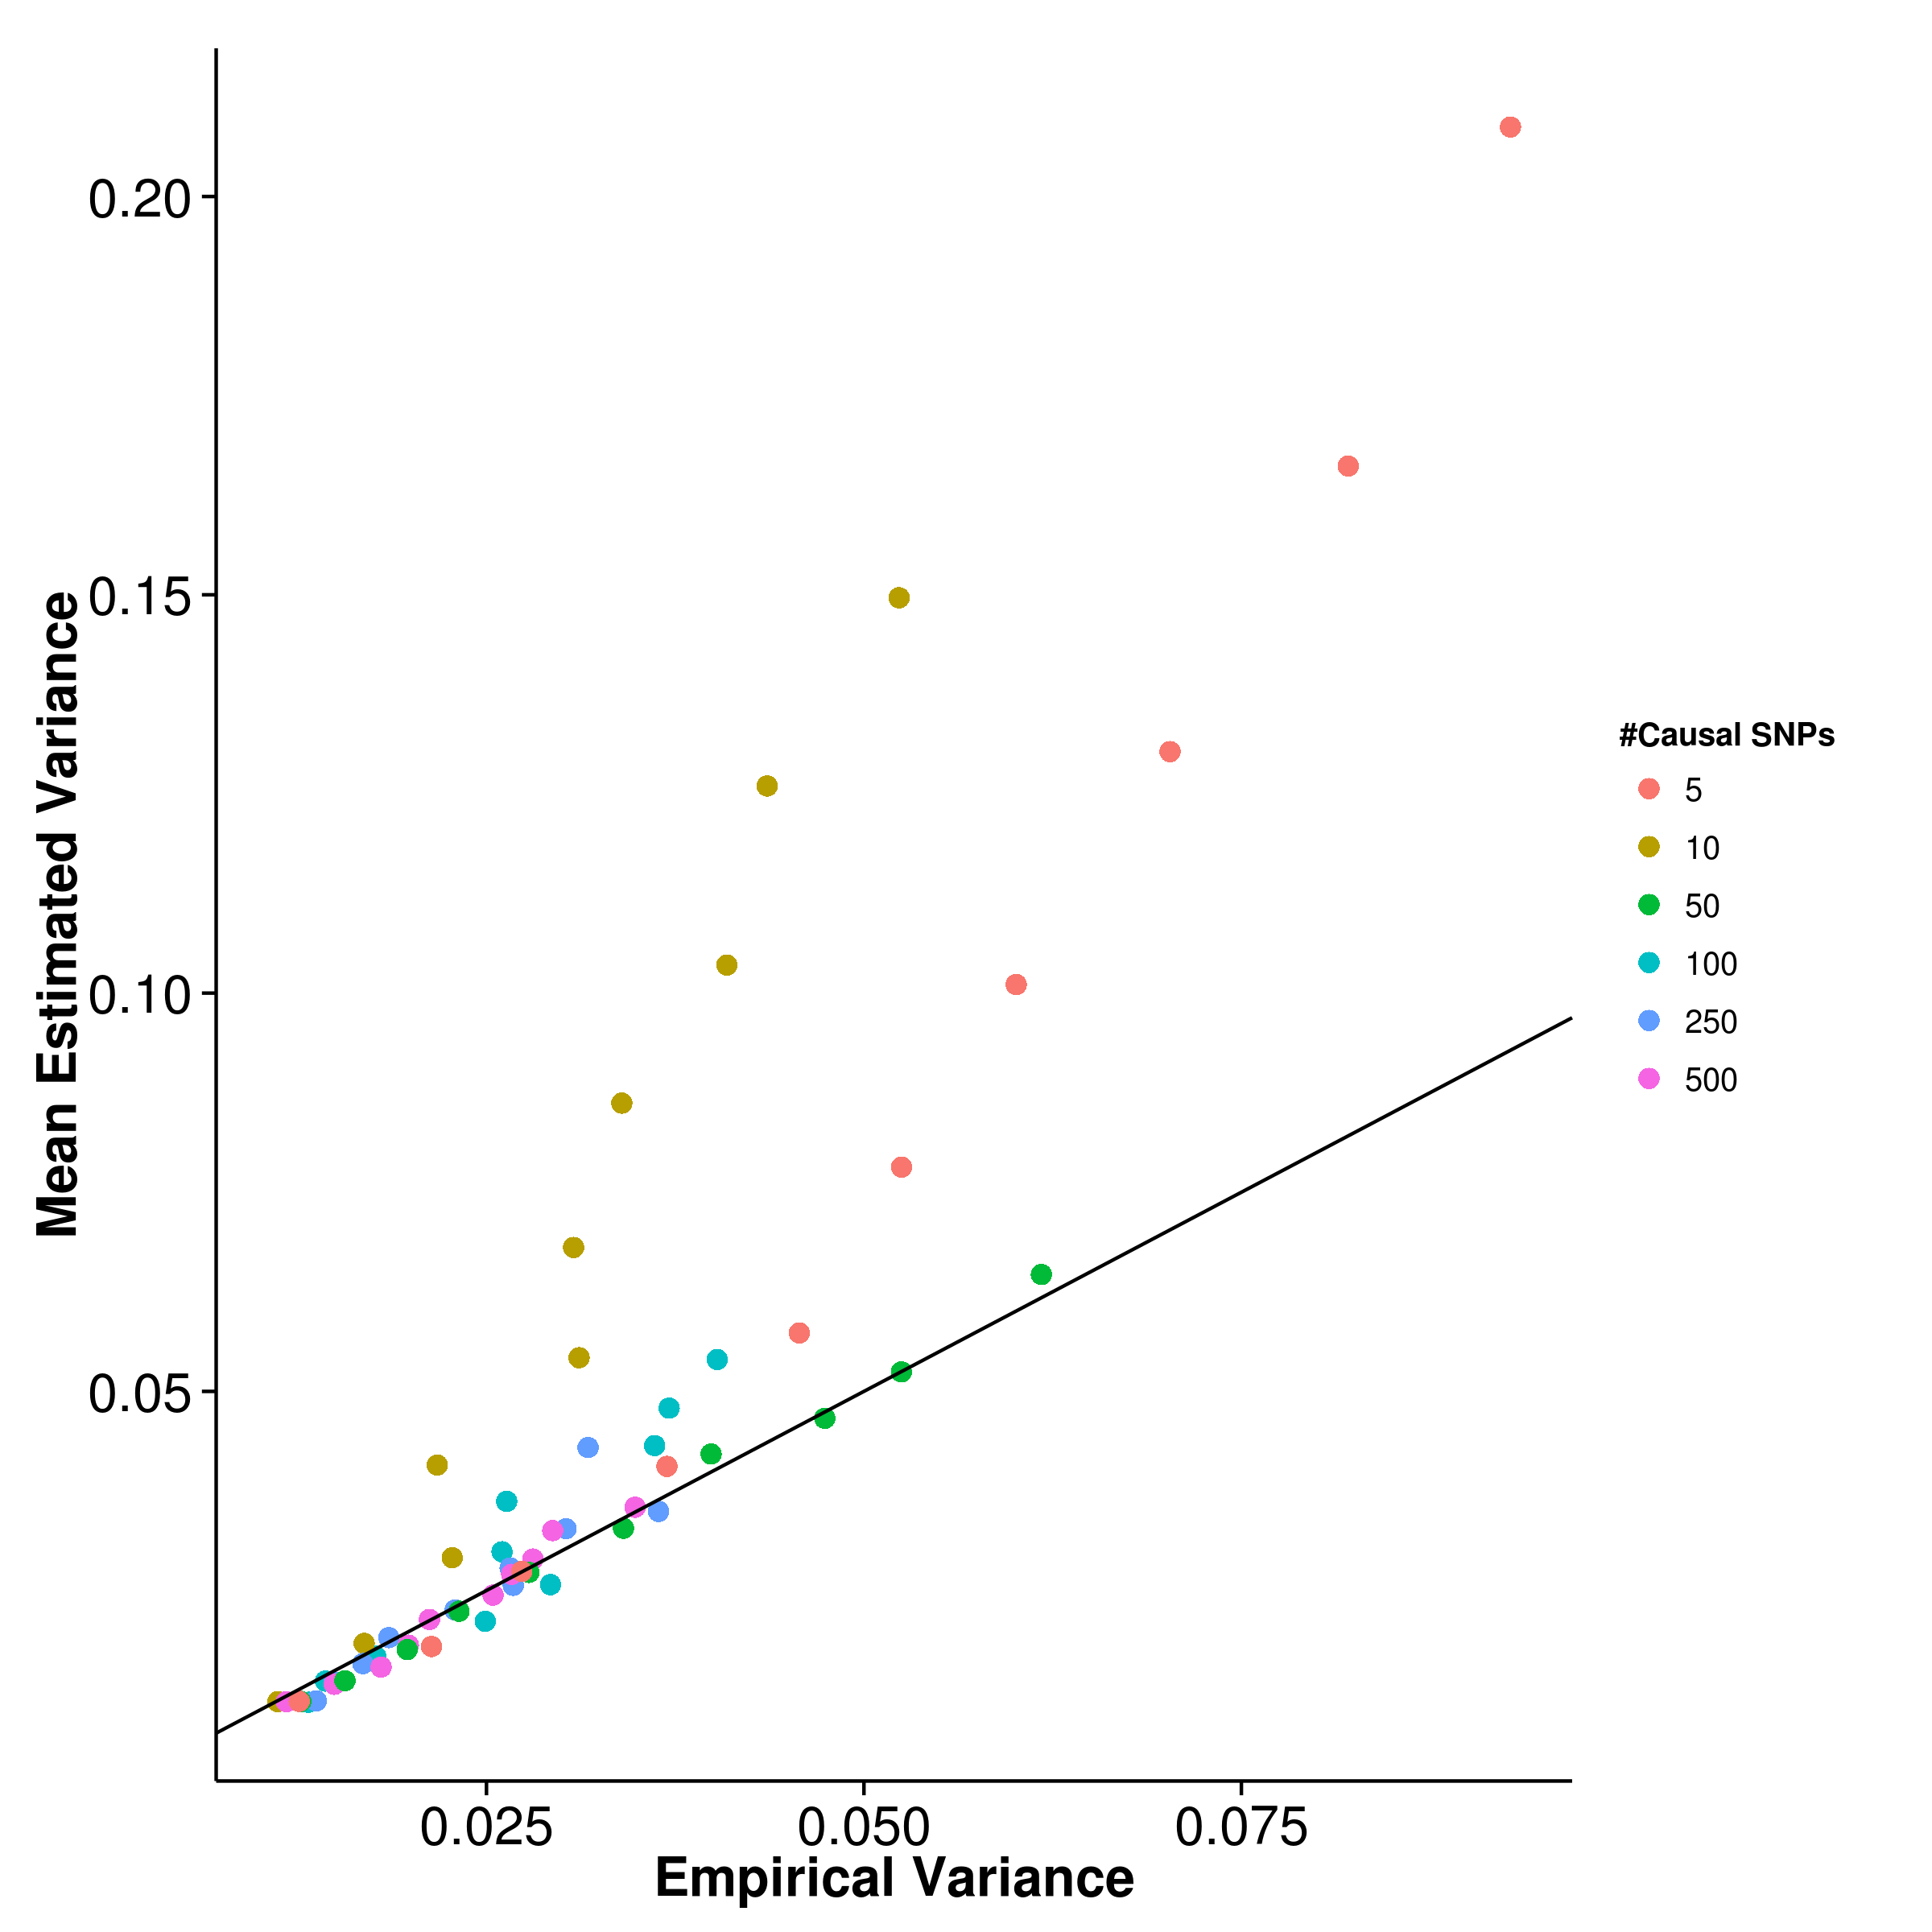
\includegraphics{figure/he_summary/equal/ldscIn_Qt_Equal_sdCom.png}}
				\label{fig:ldscInQtEqualVarCom}
			}
			\caption[Quantitative Trait with Equal Effect Size Simulation Result(Estimated Variance)]
			{Estimated variance of results from quantitative trait simulation with equal effect size simulation compared to the empirical variance.
				The estimated variances of all the tools were rather sensitive to the number of causal \glspl{SNP}, where \gls{ldsc} tends to over-estimate the variance as the number of causal \glspl{SNP} decreases and \gls{shrek} and \gls{gcta} tends to under-estimate the variance.} 
			\label{fig:QtEqualVarCom}
		\end{figure}
		The simulation of equal effect size serves as a simplistic baseline model for the performance of the programmes.
		The first thing to look at is the mean estimation of heritability of the programmes.
		If there is any bias in the estimation of the programmes, one can easily visualize it by plotting the mean estimated heritability against the simulated heritability(\cref{fig:QtEqualMean}).
		
		From the graph, it is clear that there was a slight over estimation for \gls{ldsc} with fixed intercept(\cref{fig:ldscQtEqualMean}).
		The over estimation seems to be a function of the simulated heritability, where a large inflation was observed when a larger heritability was simulated.
		On the other hand, when allow for the estimation of intercept, less bias was observed for \gls{ldsc} except for the scenario where only 5 causal \glspl{SNP} was simulated where the estimation was downwardly biased.
		
		Comparing to \gls{ldsc}, \gls{shrek} has a smaller bias and tends to slightly under-estimate(\cref{fig:shrekQtEqualMean}).
		However, the bias of \gls{shrek} is insensitive to the simulated heritability, making it robust to traits with different heritability.
		Similarly, the bias of \gls{gcta} is also smaller than that of \gls{ldsc}(\cref{fig:shrekQtEqualMean}), with a slight upward bias in the estimation except when 5 causal \glspl{SNP} was simulated.
		Again, the estimate of \gls{gcta} is also relatively insensitive to the simulated heritability.
		Overall, there was no clear pattern as to how the number of causal \glspl{SNP} affects the mean estimation. 
		
		Next, we examine the empirical variance of the programmes(\cref{fig:QtEqualVar}).
		As can be seen from the graph, there is a clear pattern where the decrease in number of causal \gls{SNP} generally increases the variance for all the programmes, with \gls{shrek} least affected.
		For \gls{ldsc}, the simulated heritability also have a large impact to its empirical variance, with the empirical variance increases as the simulated heritability increases.
		In general, \gls{ldsc} with fixed intercept(\cref{fig:ldscQtEqualVar}) has a lower variance when compared to \gls{ldsc} with intercept estimation(\cref{fig:ldscInQtEqualVar}). 
		Moreover, when the number of causal \gls{SNP} is large, the variance of \gls{ldsc} with fixed intercept(\cref{fig:ldscQtEqualVar}) is lower than \gls{shrek}(\cref{fig:shrekQtEqualVar}).
		However, \gls{shrek} is more robust to change in the number of causal \glspl{SNP} and simulated heritabiliy when compared ot \gls{ldsc}.

		Of all the programmes, \gls{gcta} has the best performance(\cref{fig:gctaQtEqualVar}) except when the trait only contains 5 causal \glspl{SNP}. 
		Not only does it has the smallest variance, its empirical variances was almost invariant to change in simulated heritability.
		However, the case with 5 causal \glspl{SNP} serves as an out-lier. 
		It was most obvious when inspecting the relationship between the estimated variance and the empirical variance of \gls{gcta}(\cref{fig:gctaQtEqualVarCom}).
		Comparing the estimated variance and the empirical variance, it was clear that \gls{gcta} can, in most case accurately estimate its variance. 
		In the case of 5 causal \glspl{SNP} however, \gls{gcta} underestimates its variance.
		It was also observed in the case of 10 causal \glspl{SNP}, there was already a slight under-estimation of the variance, suggesting that there might be an increase in empirical variance that was not capture by \gls{gcta}.
		
		In the case of the programmes using the test statistic, it was observed that \gls{shrek} in general under-estimate the empirical variance(\cref{fig:shrekQtEqualVarCom}) for an average of 0.9 fold. 
		On the other hand, \gls{ldsc} over-estimates the variance for roughly 1.5 times when a fixed intercept(\cref{fig:ldscQtEqualVarCom}) was used and roughly 1.2 times when the intercept was estimated(\cref{fig:ldscInQtEqualVarCom}). 
		
		To summarize the results, we calculate the \gls{mse} of the estimation of heritability of the programmes under different simulation condition(\cref{tab:mseQtEqual}). 
		With the exception of the 5 causal \glspl{SNP} scenario, \gls{gcta} has the best performance, has a almost 2 fold smaller \gls{mse} when compared to \gls{shrek}.
		As the number of casual \glspl{SNP} increases, the performance of \gls{ldsc} with fixed intercept and \gls{shrek} converges where in general, \gls{shrek} has a smaller \gls{mse}.
		Interestingly, unlike \gls{ldsc}, \gls{shrek} was insensitive to change in number of causal \glspl{SNP} and its performance were relatively stable.
		
		% Describe the mean
		% Effect of heritability on the mean estimation
		% Effect of causal SNPs on the mean estimation
		% Descript the Variance
		% Effect of heritability on variance of estimate
		% Effect of number of causal SNPs on variance of estimation
		% Describe the estimated variance
		% How the number of causal SNPs affect the estimation of variance?

		\begin{table}
			\centering
			\begin{tabular}{rrrrr}
				\toprule
				Number of Causal SNPs&	SHREK&	LDSC&	LDSC-In&	GCTA \\
				\midrule
				5	&	0.167	&	0.308&	0.526&	0.177	\\
				10	&	0.158	&	0.243&	0.337&	0.0944	\\
				50	&	0.150	&	0.163&	0.354&	0.0749	\\
				100	&	0.154	&	0.161&	0.304&	0.0664	\\
				250	&	0.157	&	0.147&	0.255&	0.0659	\\
				500	&	0.147	&	0.148&	0.247&	0.0661	\\
				\bottomrule
			\end{tabular}
			\caption[Mean Squared Error of Quantitative Trait Simulation with Equal Effect Size]{
				\gls{mse} of quantitative trait simulation with equal effect size.
				It was observed that the overall \gls{mse} of \gls{gcta} is very low, follow by \gls{shrek}.
				As the number of causal \glspl{SNP} decreases, the \gls{mse} increases for all programmes. 
				The performance of \gls{shrek} and \gls{ldsc} with fixed intercept converges as the number of causal \glspl{SNP} increases.}
			\label{tab:mseQtEqual}
		\end{table}
		
		\subsection{Quantitative Trait Simulation with Random Effect Size}
		% QT Random Effect
			\begin{figure}
			\centering
			\subfloat[SHREK]{
				\scalebox{.4}{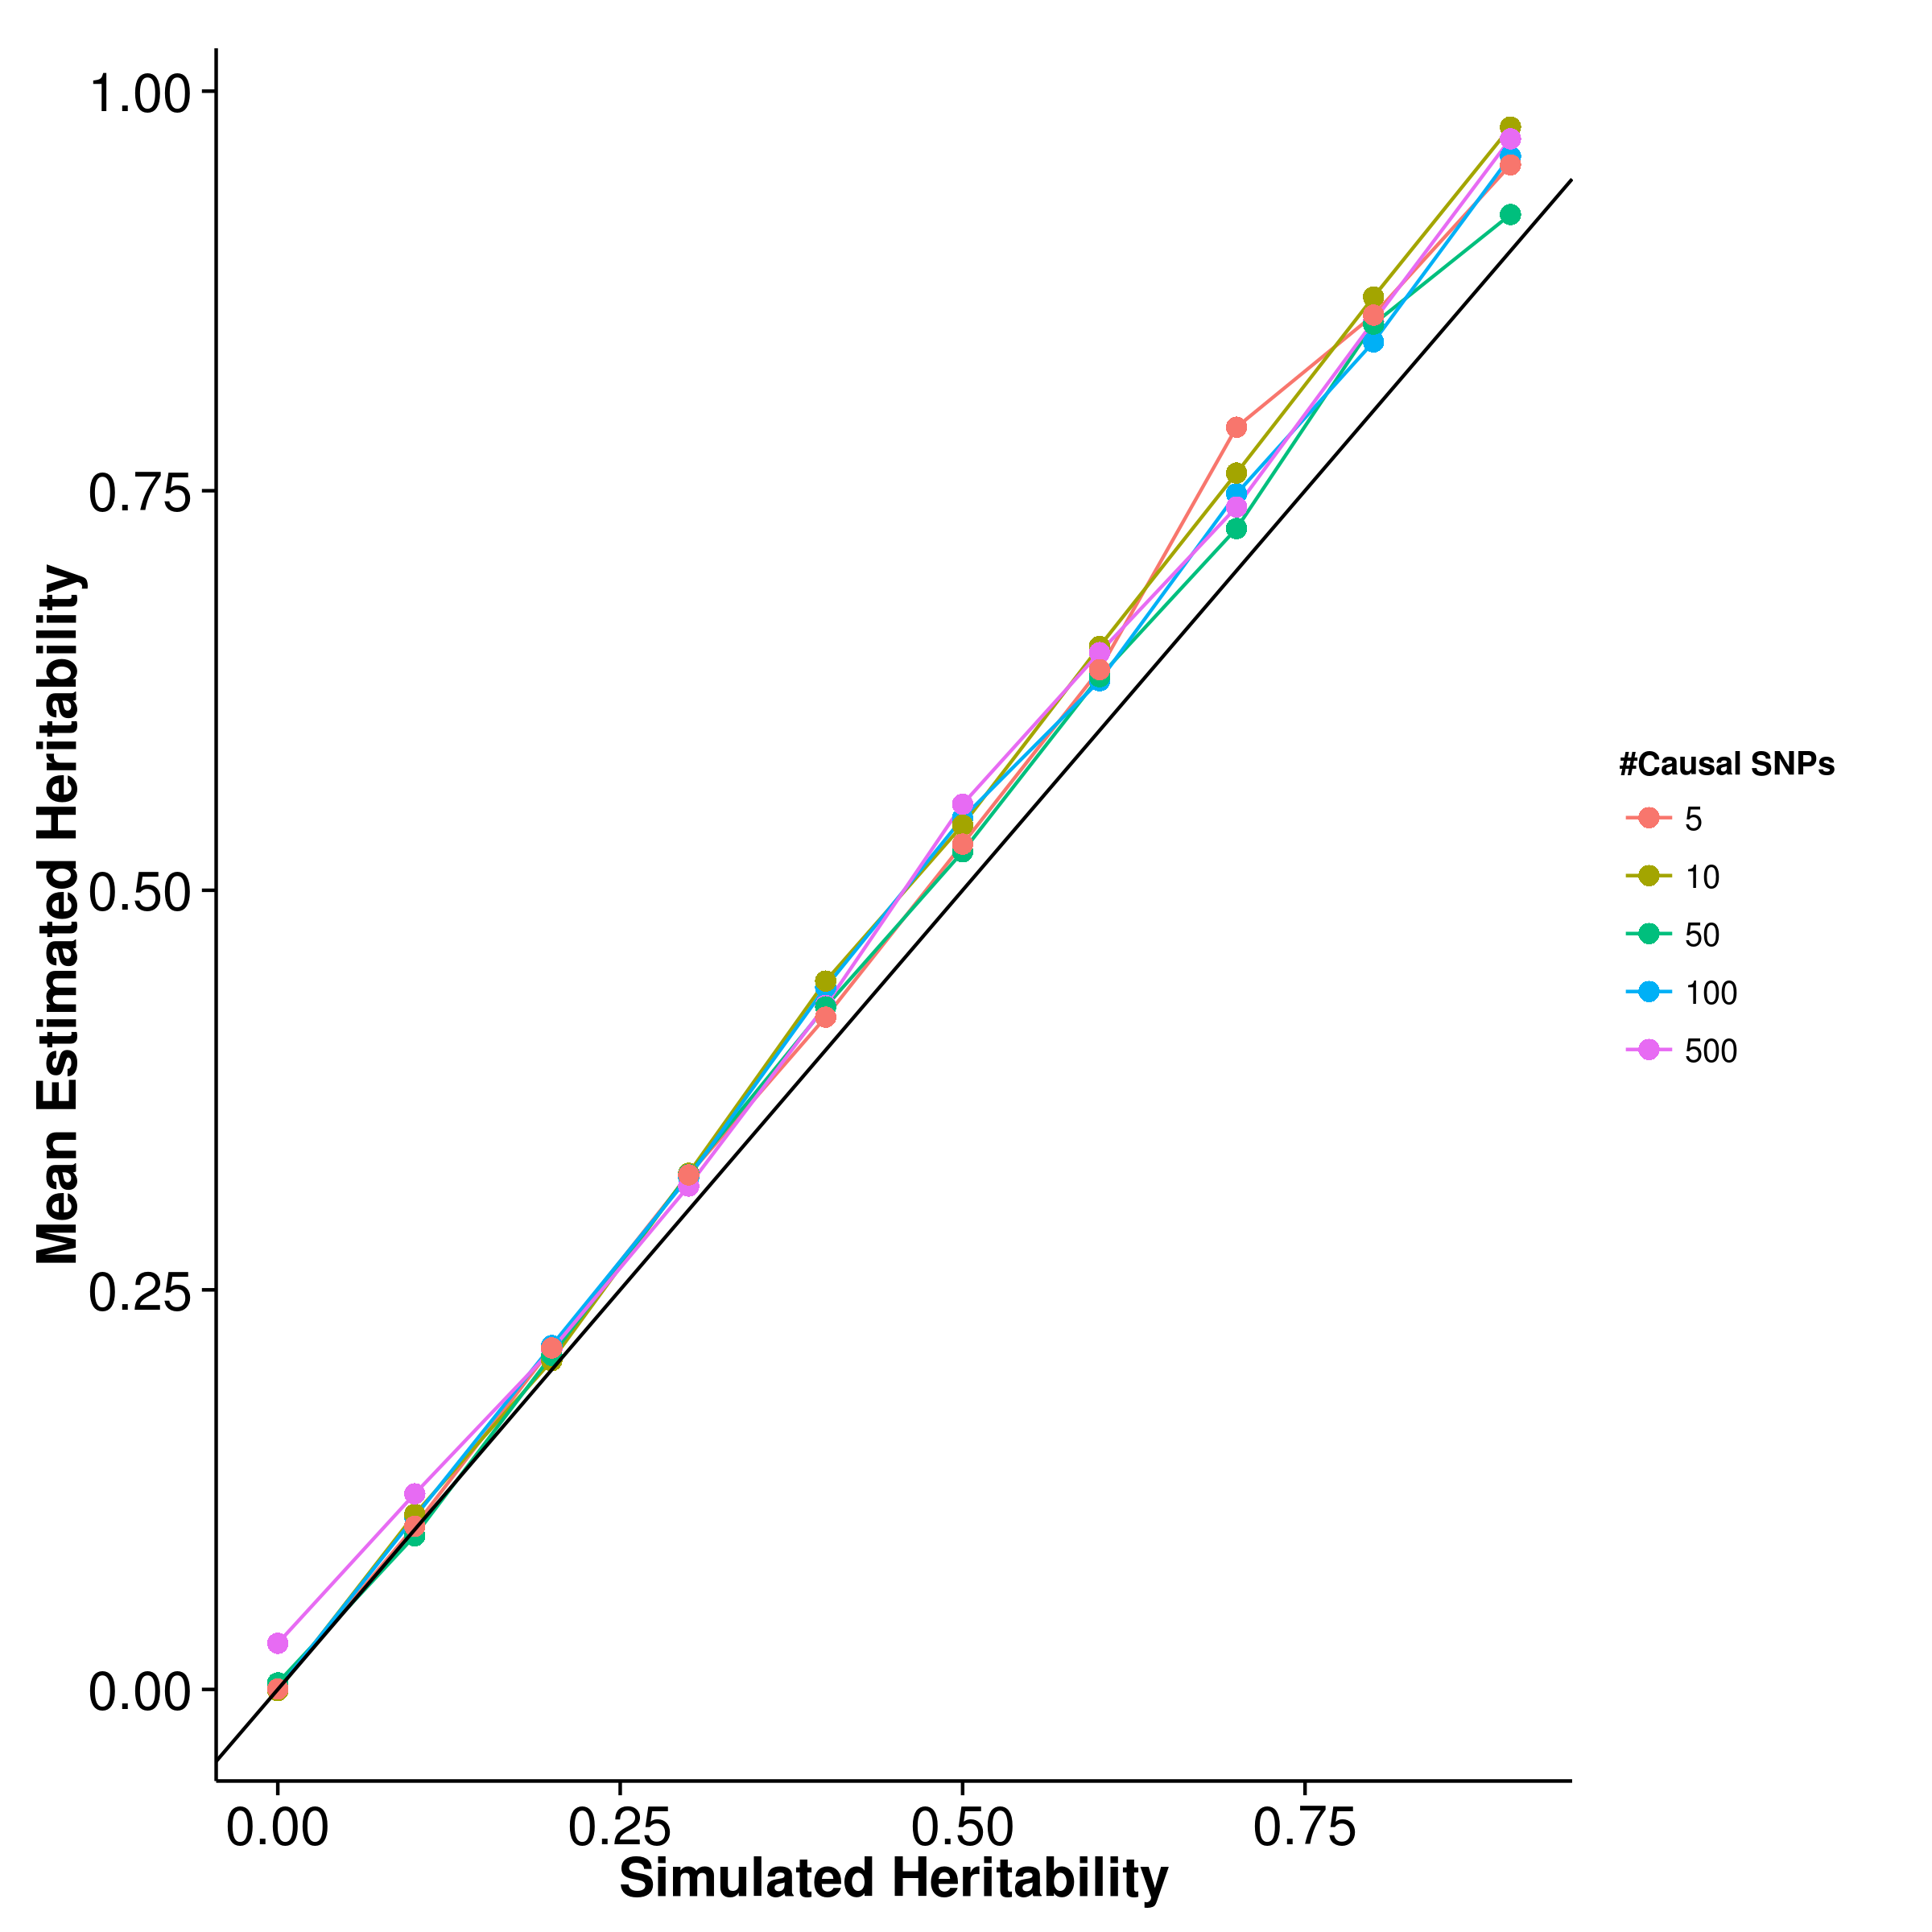
\includegraphics{figure/he_summary/random/shrek_Qt_Rand_mean.png}}
				\label{fig:shrekQtRandMean}
			}
			\subfloat[GCTA]{
				\scalebox{.4}{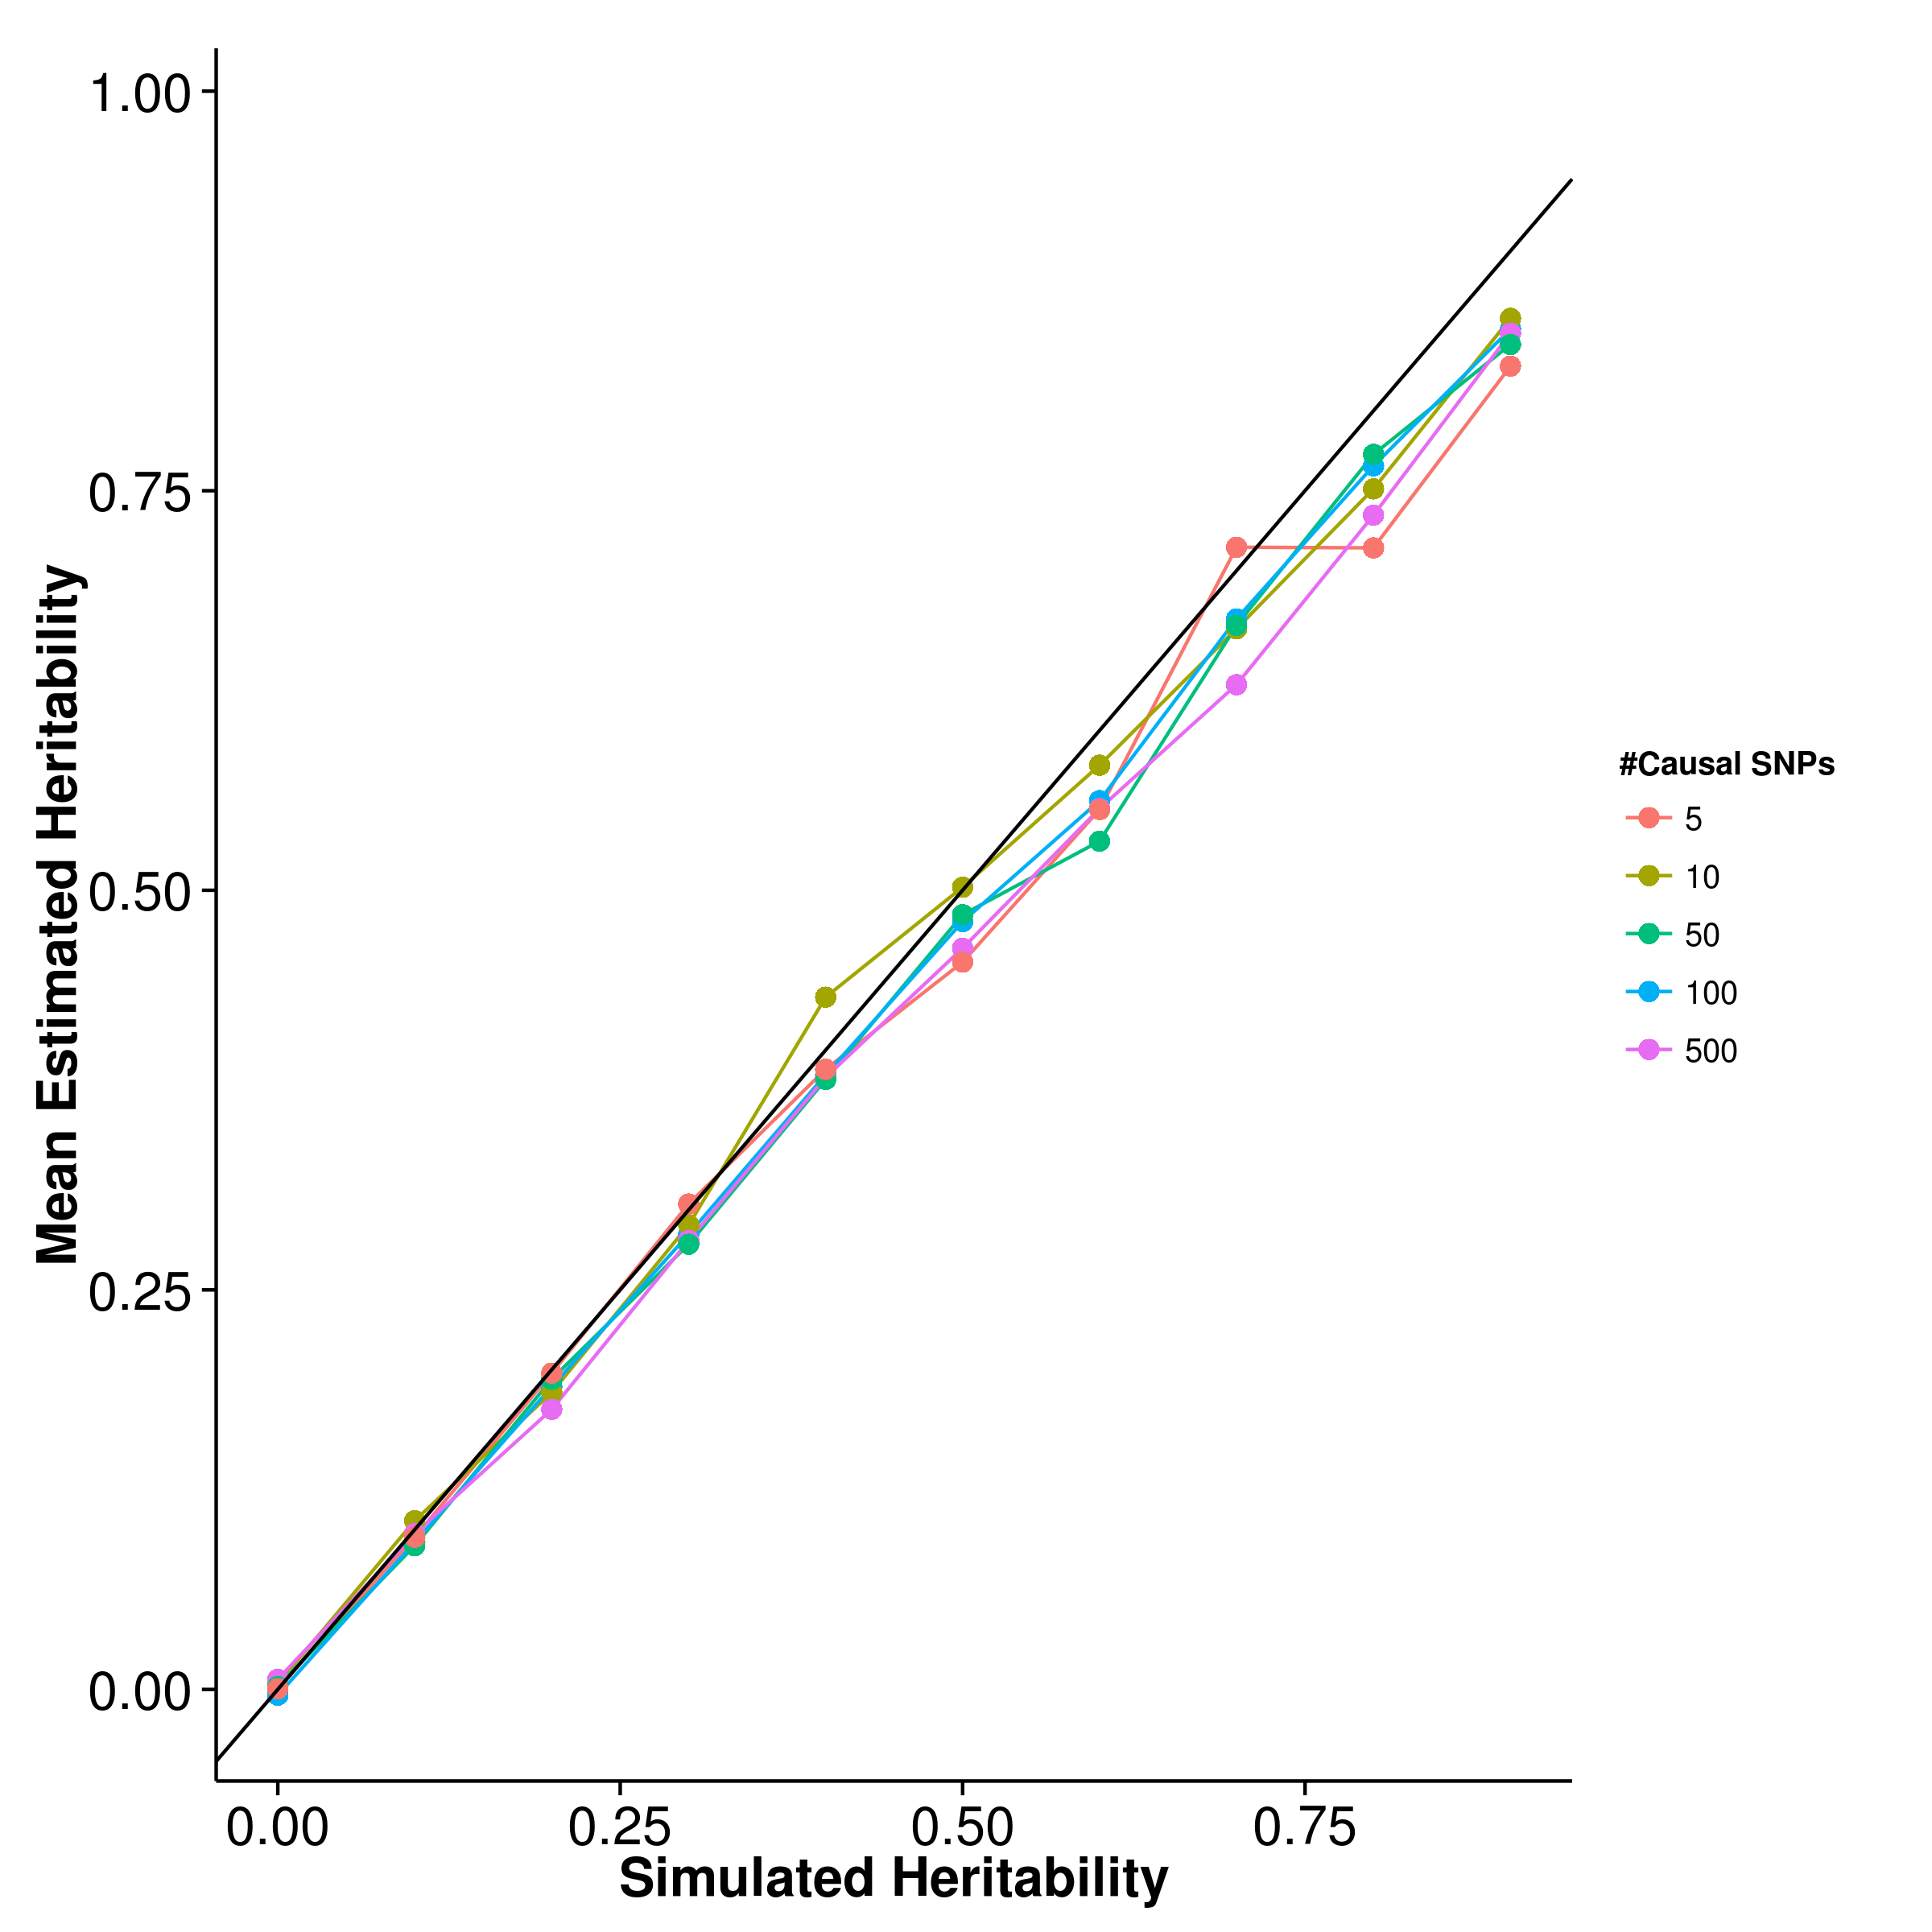
\includegraphics{figure/he_summary/random/gcta_Qt_Rand_mean.png}}
				\label{fig:gctaQtRandMean}
			}\\
			\subfloat[LDSC with fix intercept]{
				\scalebox{.4}{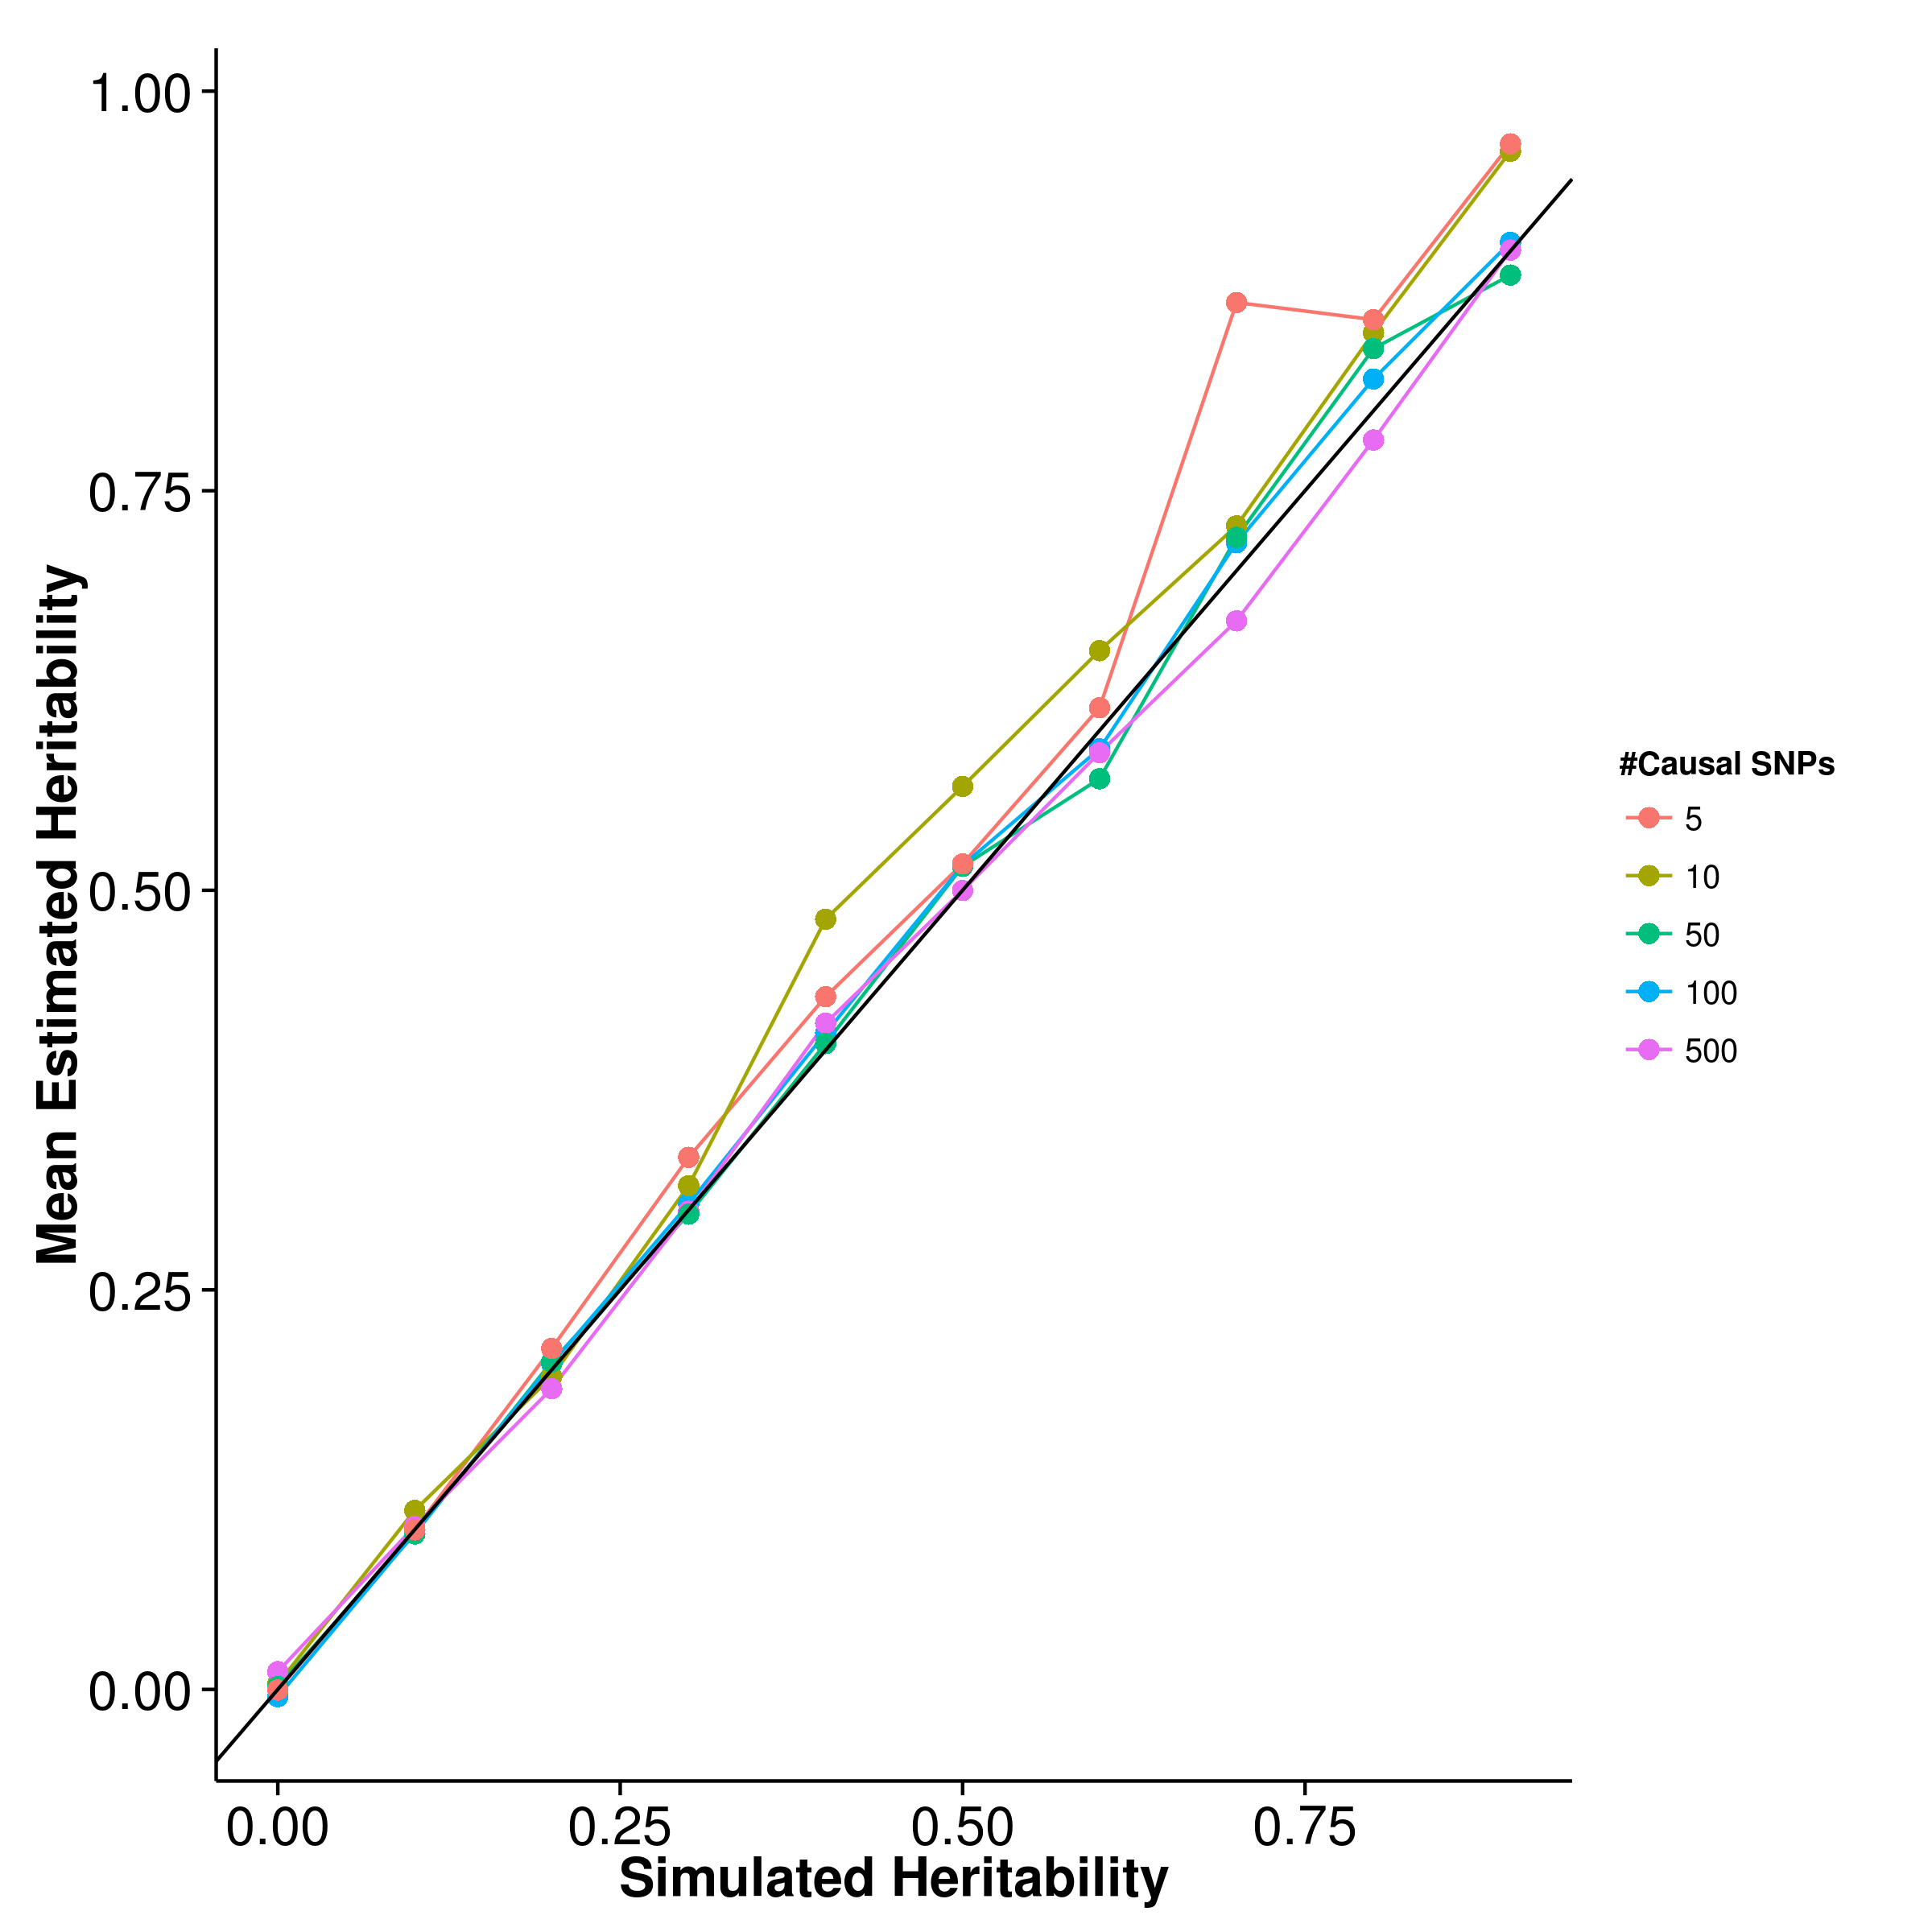
\includegraphics{figure/he_summary/random/ldsc_Qt_Rand_mean.png}}
				\label{fig:ldscQtRandMean}
			}
			\subfloat[LDSC with intercept estimation]{
				
				\scalebox{.4}{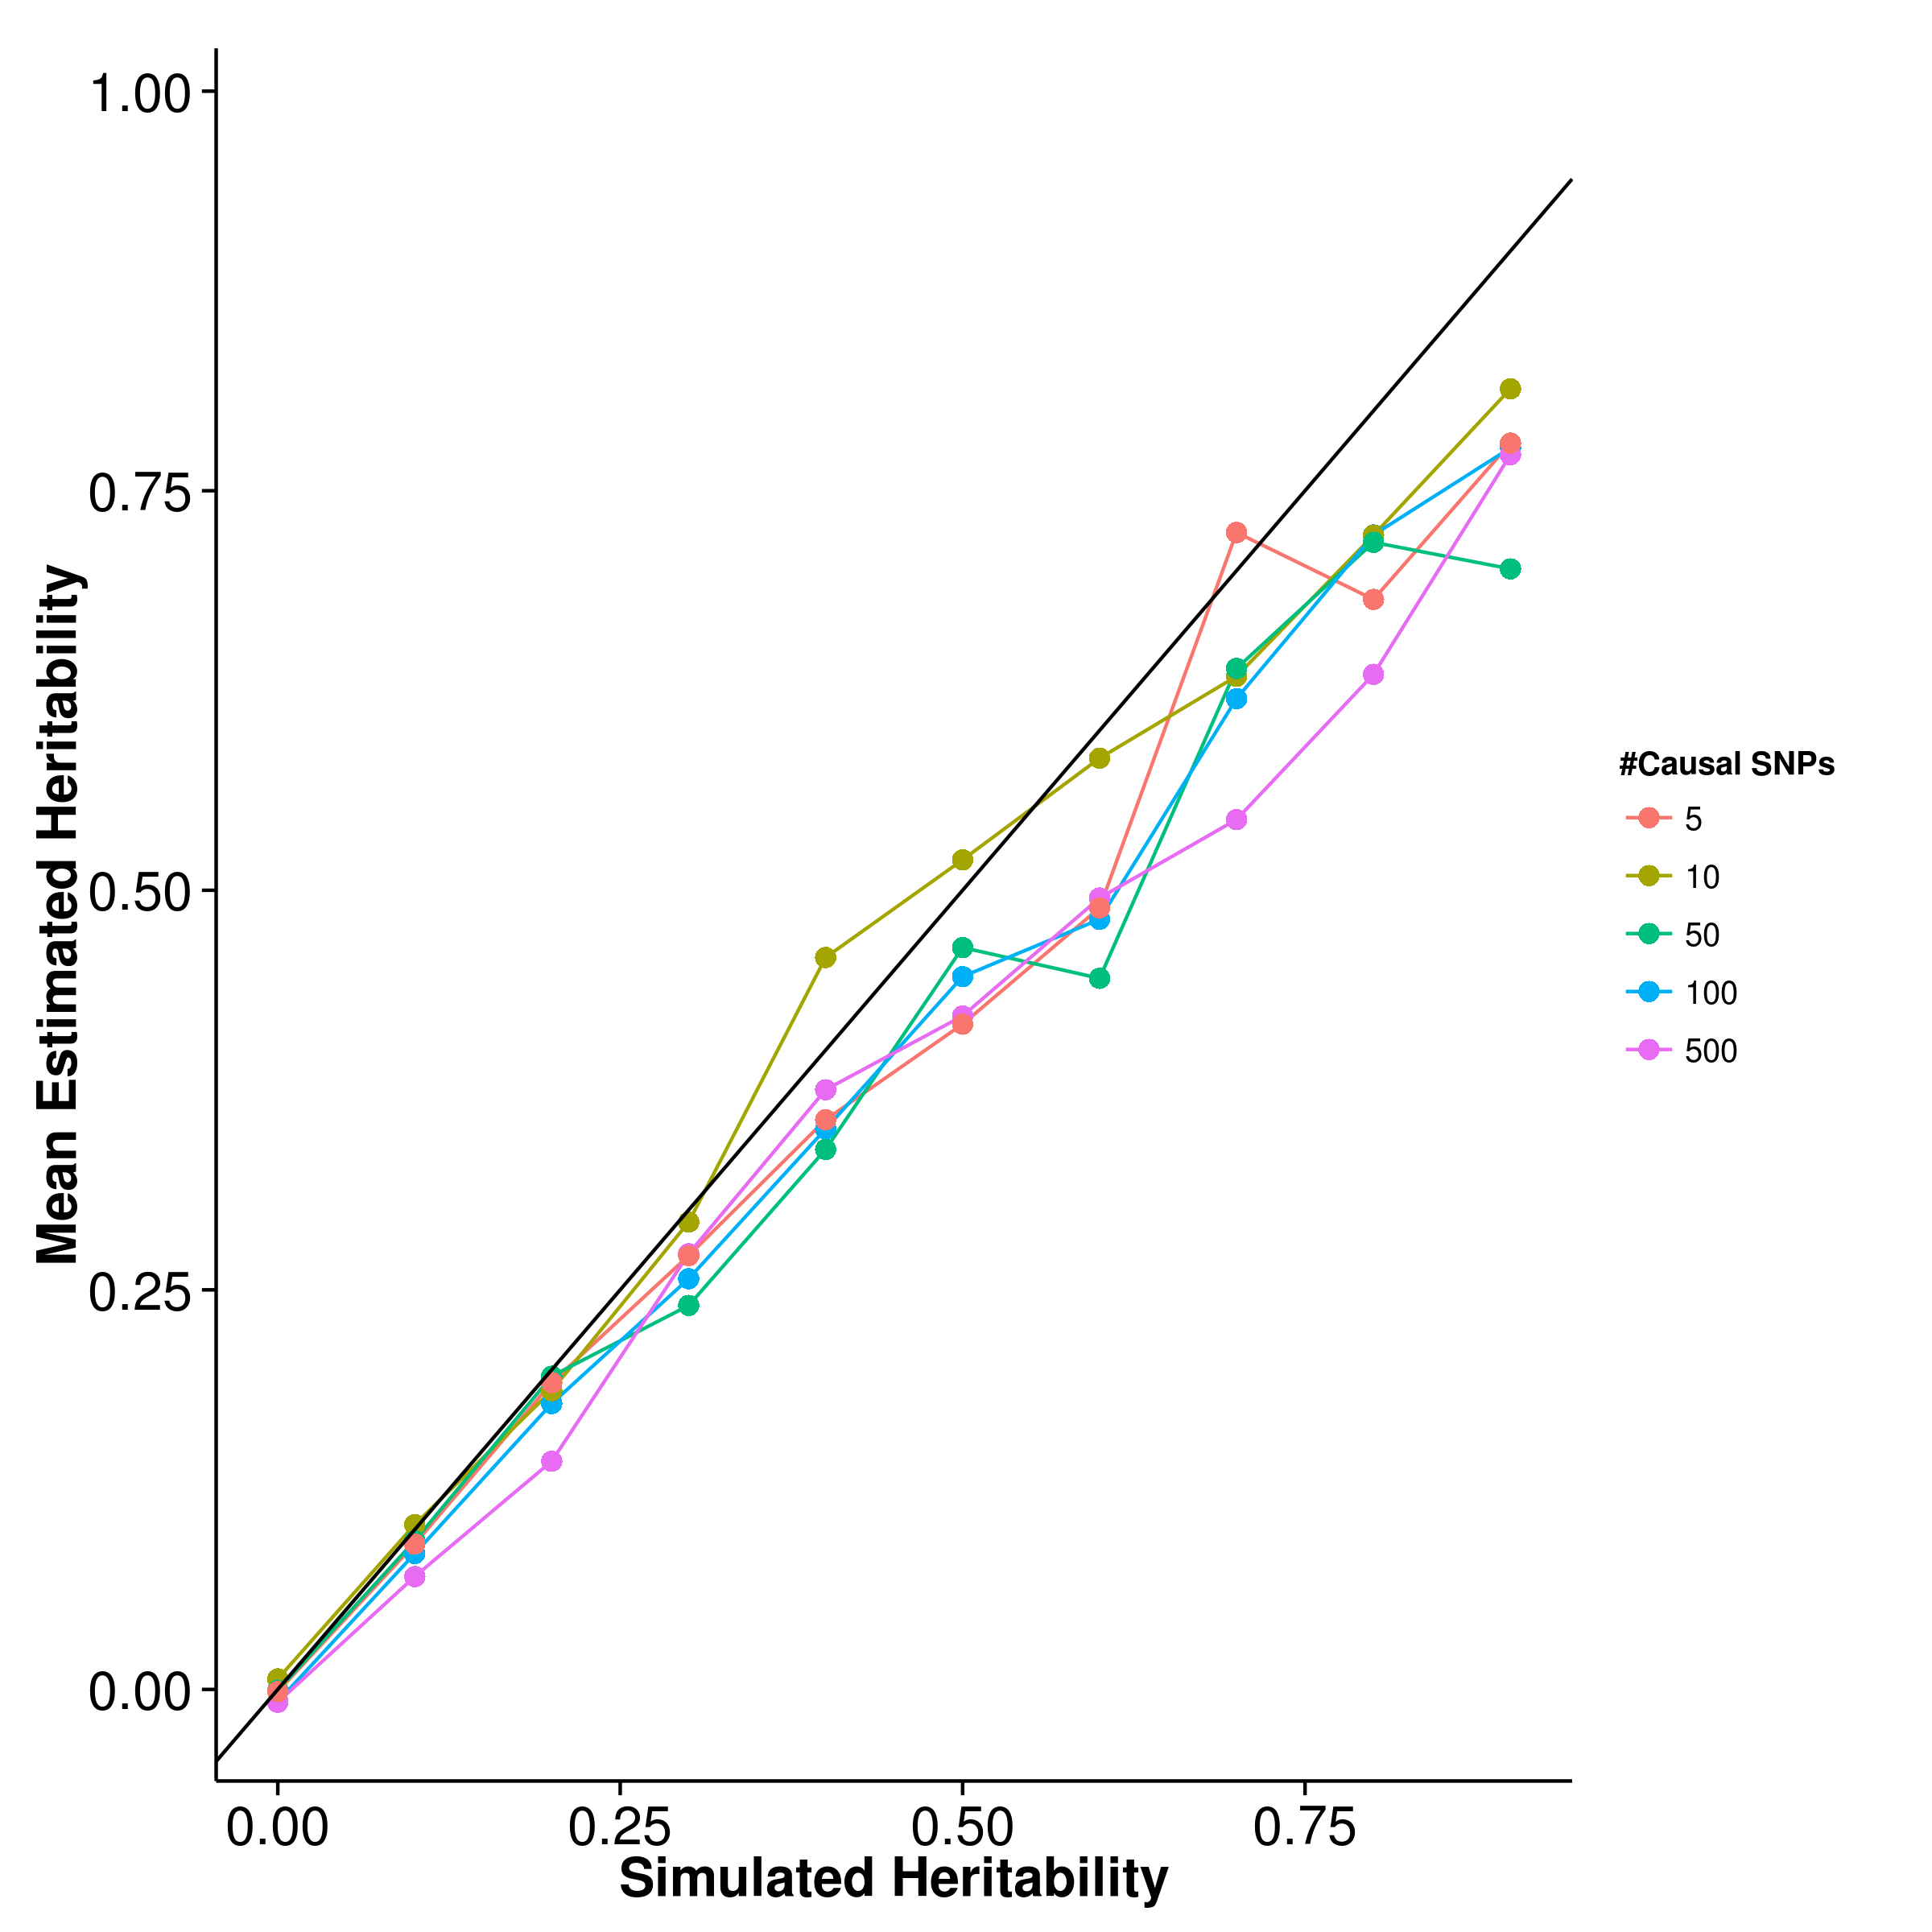
\includegraphics{figure/he_summary/random/ldscIn_Qt_Rand_mean.png}}
				\label{fig:ldscInQtRandMean}
			}
			\caption[Mean of Quantitative Trait Simulation Results]
			{Mean of results from quantitative trait simulation with random effect size simulation.
				Estimations form \gls{shrek} were slightly biased upwards whereas \gls{gcta} and \gls{ldsc} with intercept estimations both biased downwards.
				On the other hand, \gls{ldsc} with fixed intercept provides least biased estimates under polygenic conditions. 
				However, when the number of causal \glspl{SNP} is small (e.g. 5 or 10), an upward bias was observed.} 
			\label{fig:QtRandMean}
		\end{figure}
		
		\begin{figure}
			\centering
			\subfloat[SHREK]{
				\scalebox{.4}{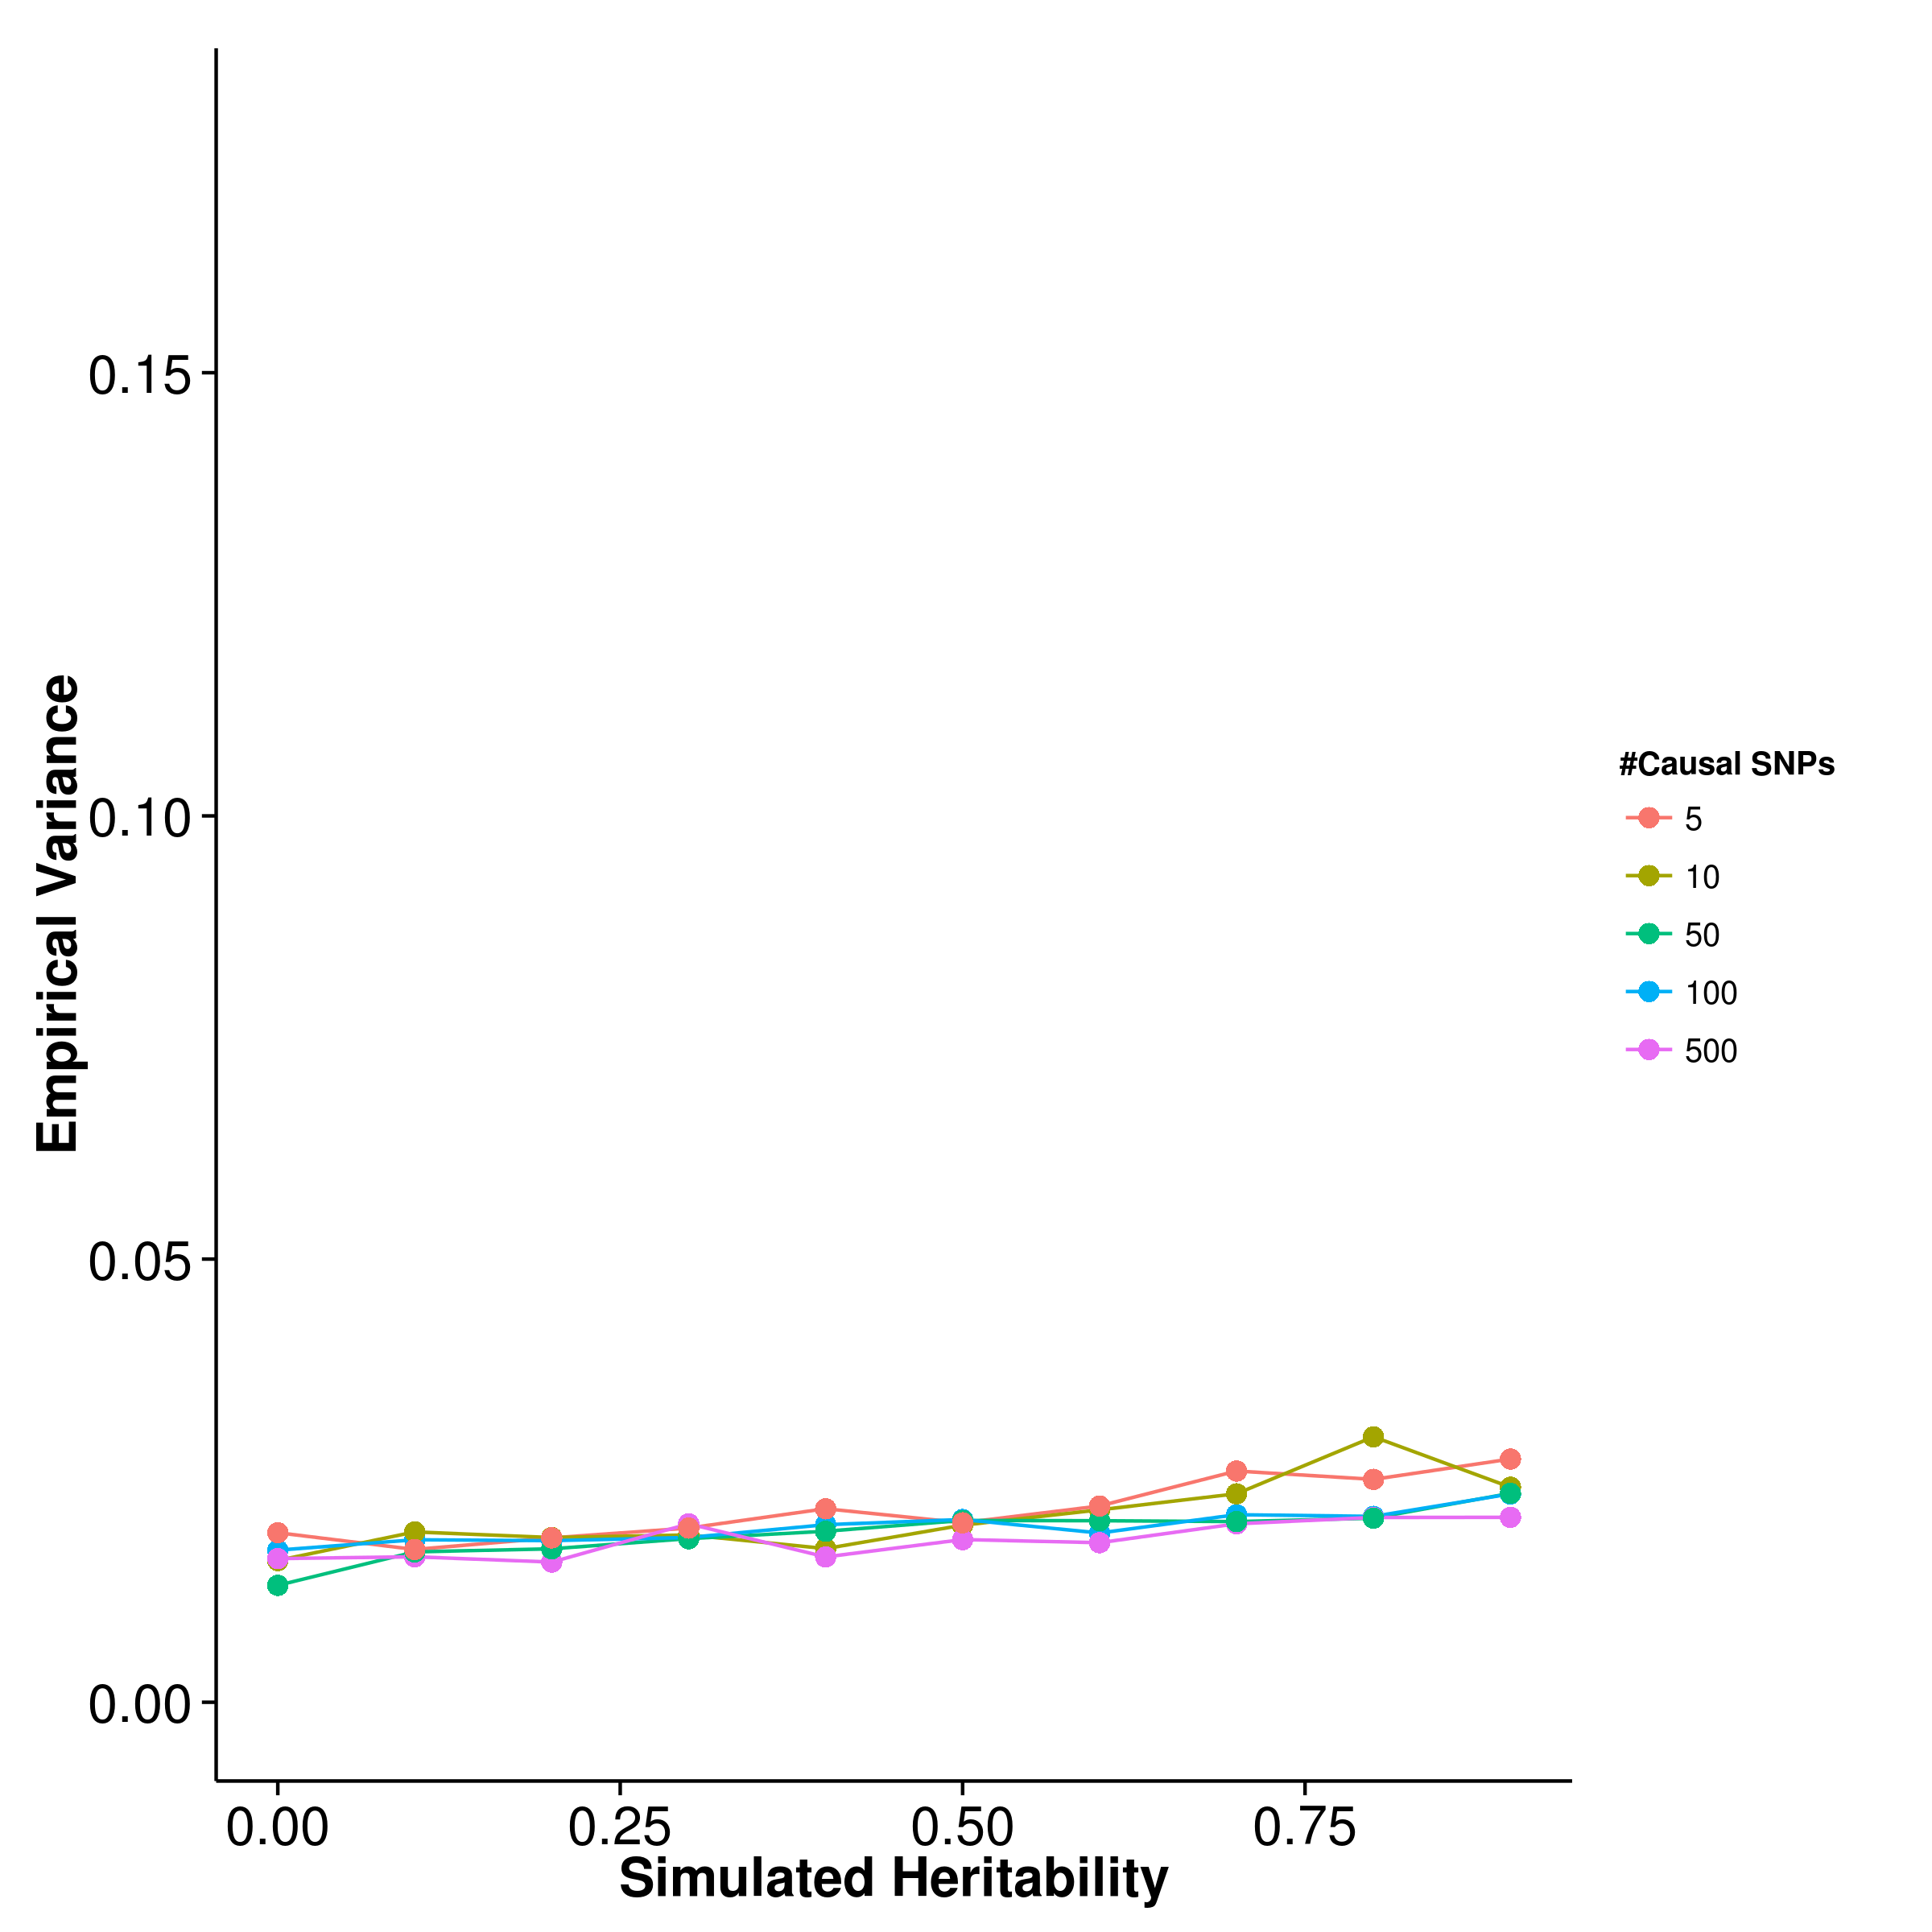
\includegraphics{figure/he_summary/random/shrek_Qt_Rand_sd.png}}
				\label{fig:shrekQtRandVar}
			}
			\subfloat[GCTA]{
				\scalebox{.4}{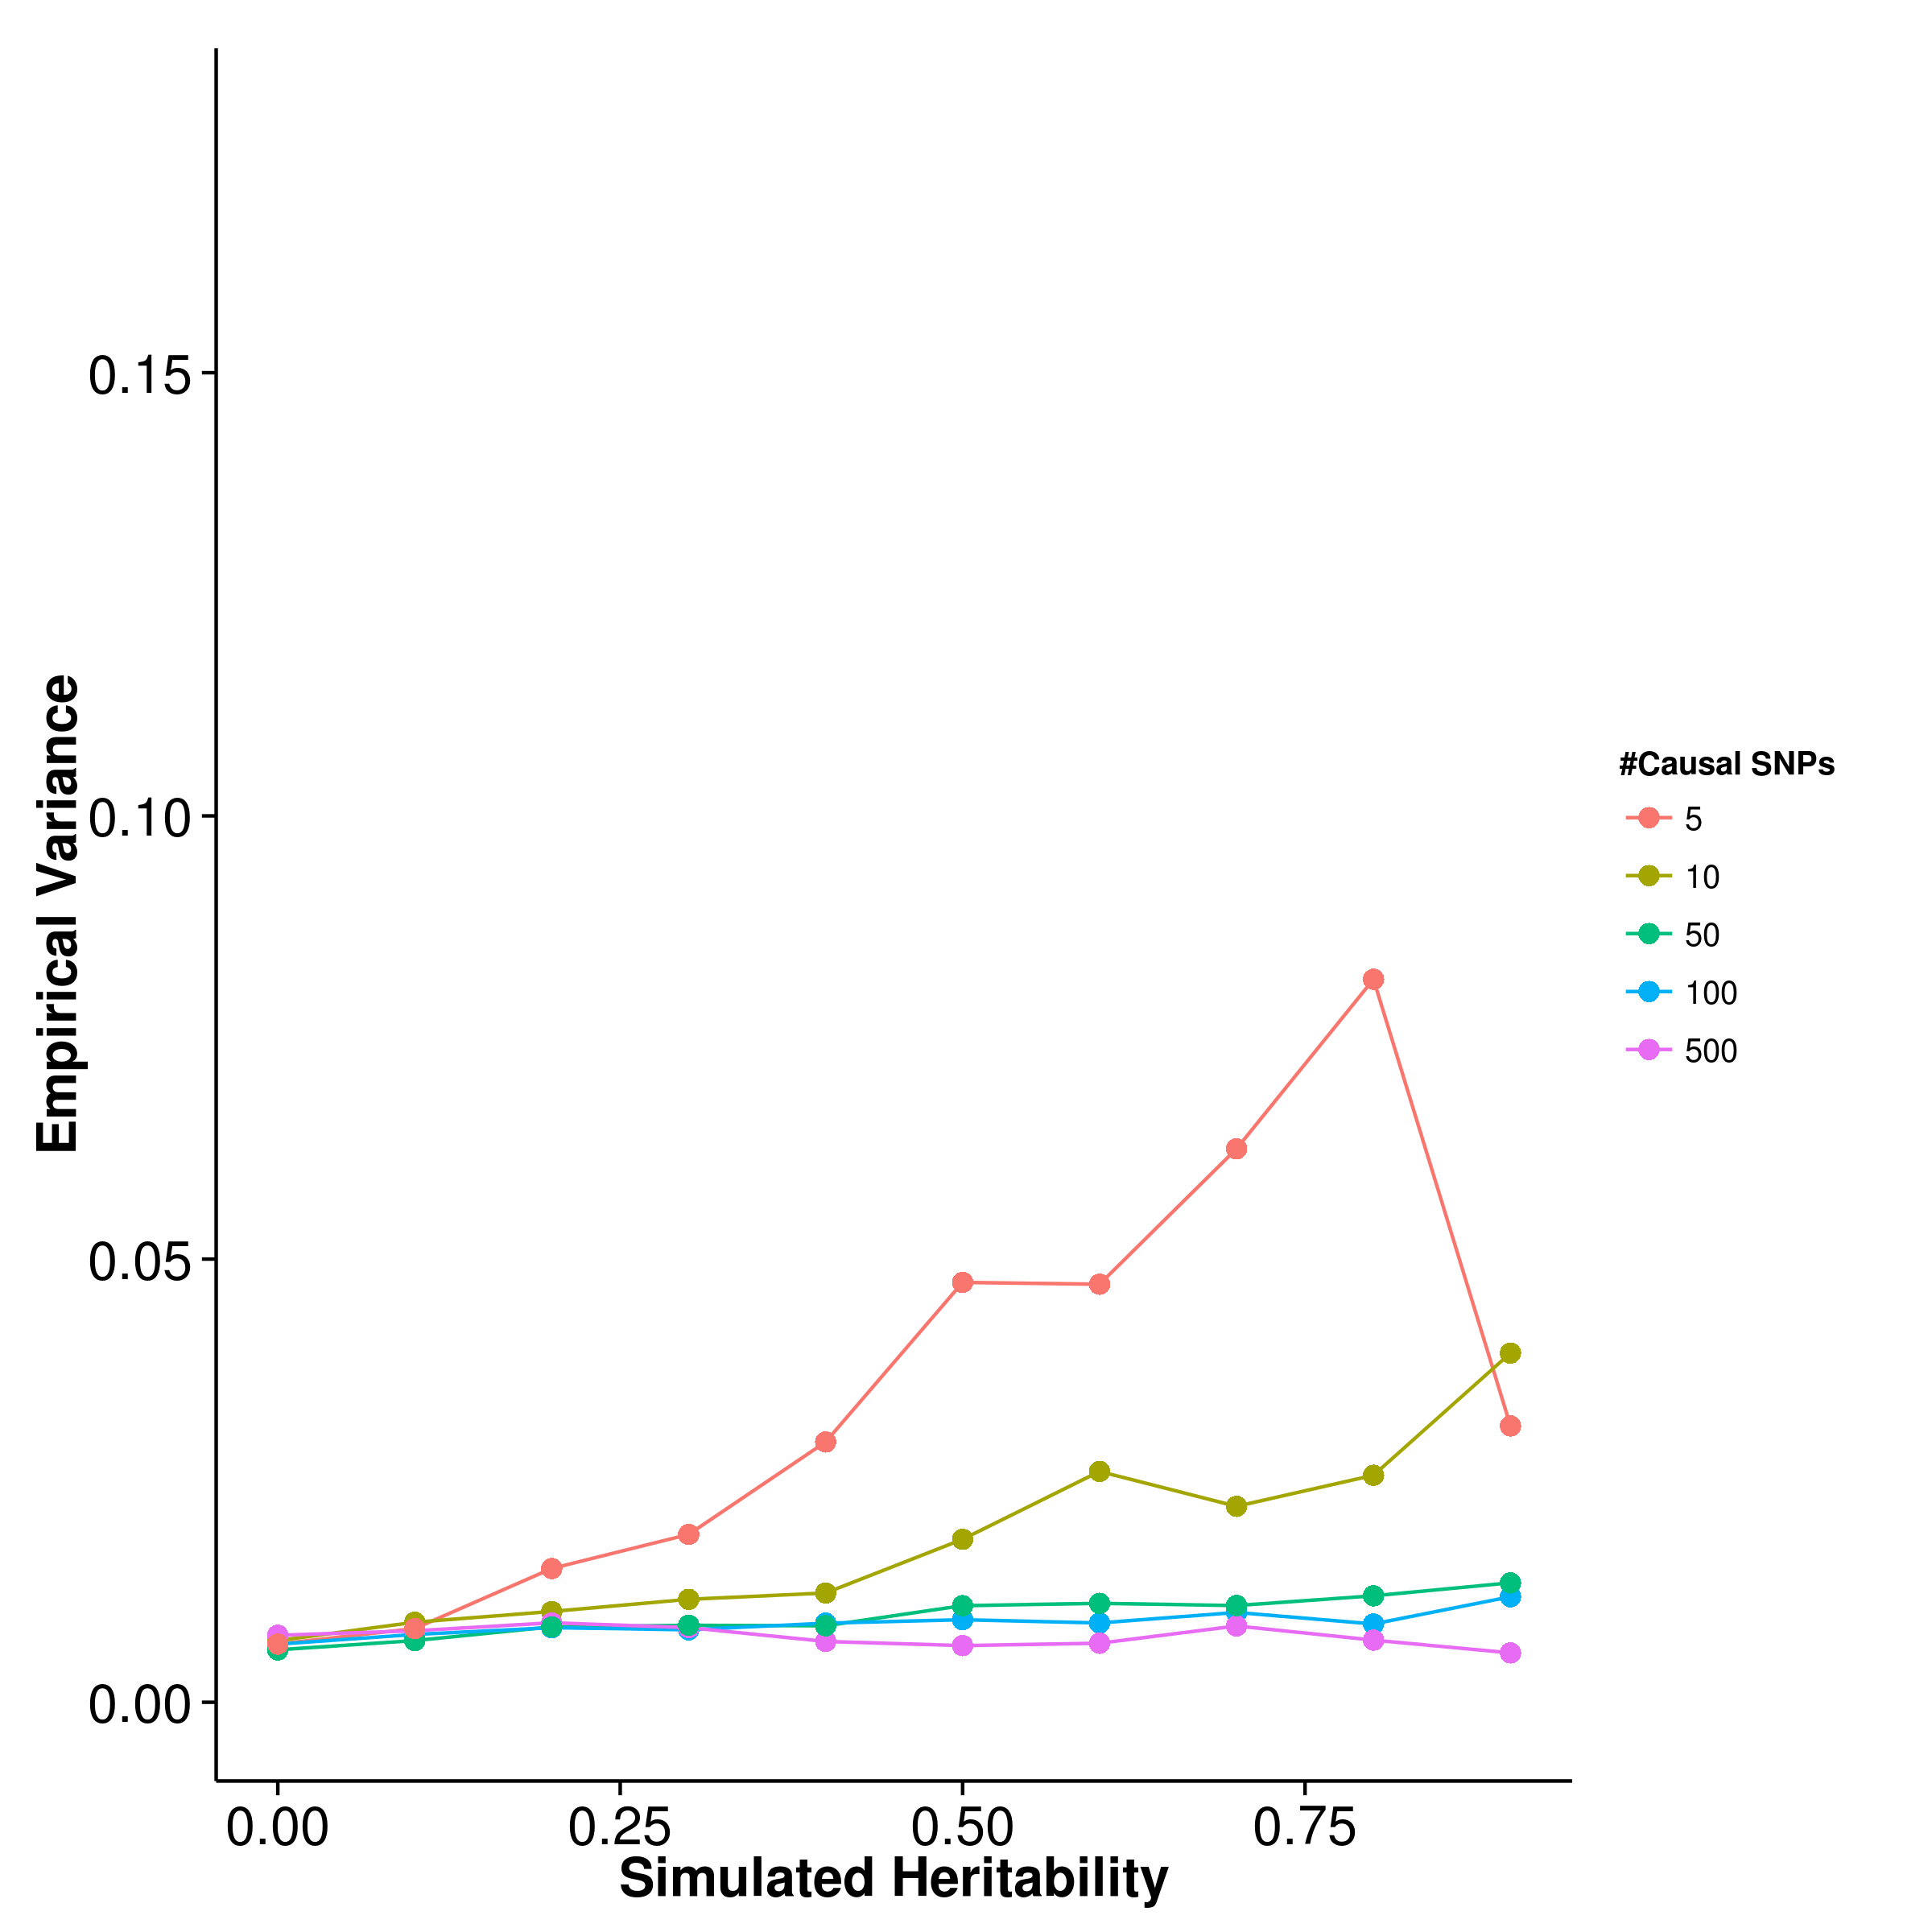
\includegraphics{figure/he_summary/random/gcta_Qt_Rand_sd.png}}
				\label{fig:gctaQtRandVar}
			}\\
			\subfloat[LDSC with fix intercept]{
				\scalebox{.4}{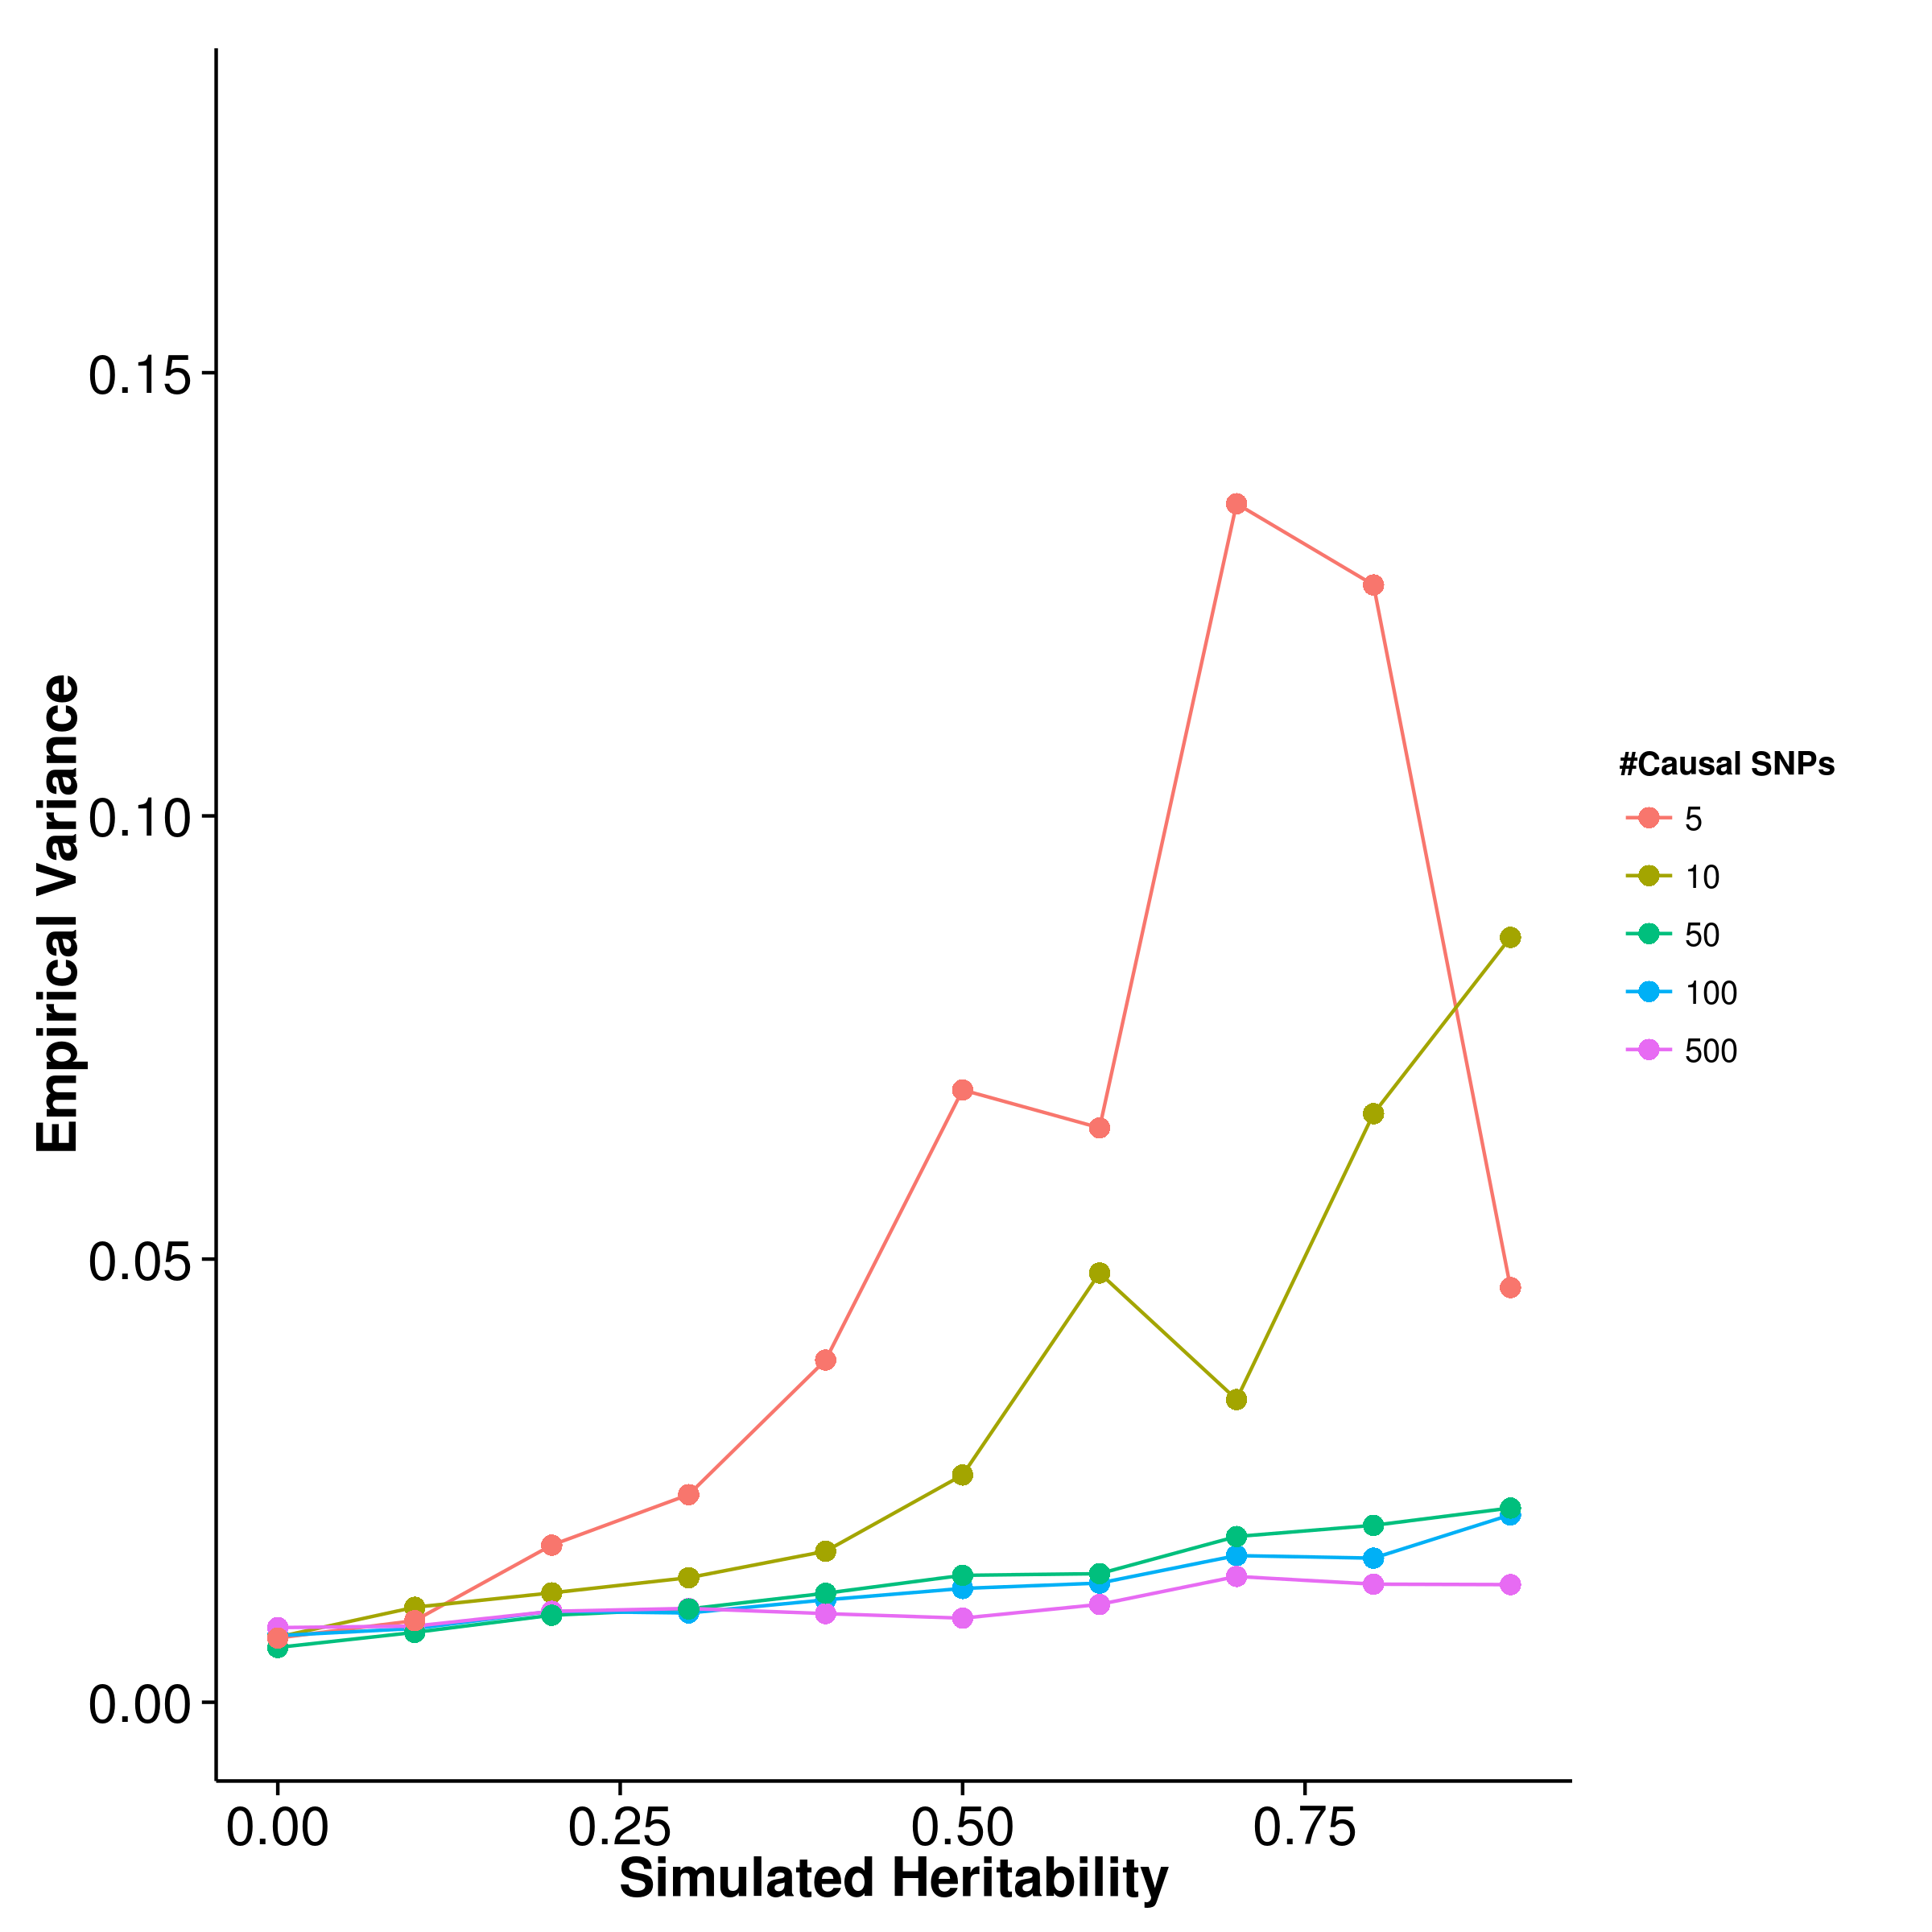
\includegraphics{figure/he_summary/random/ldsc_Qt_Rand_sd.png}}
				\label{fig:ldscQtRandVar}
			}
			\subfloat[LDSC with intercept estimation]{
				
				\scalebox{.4}{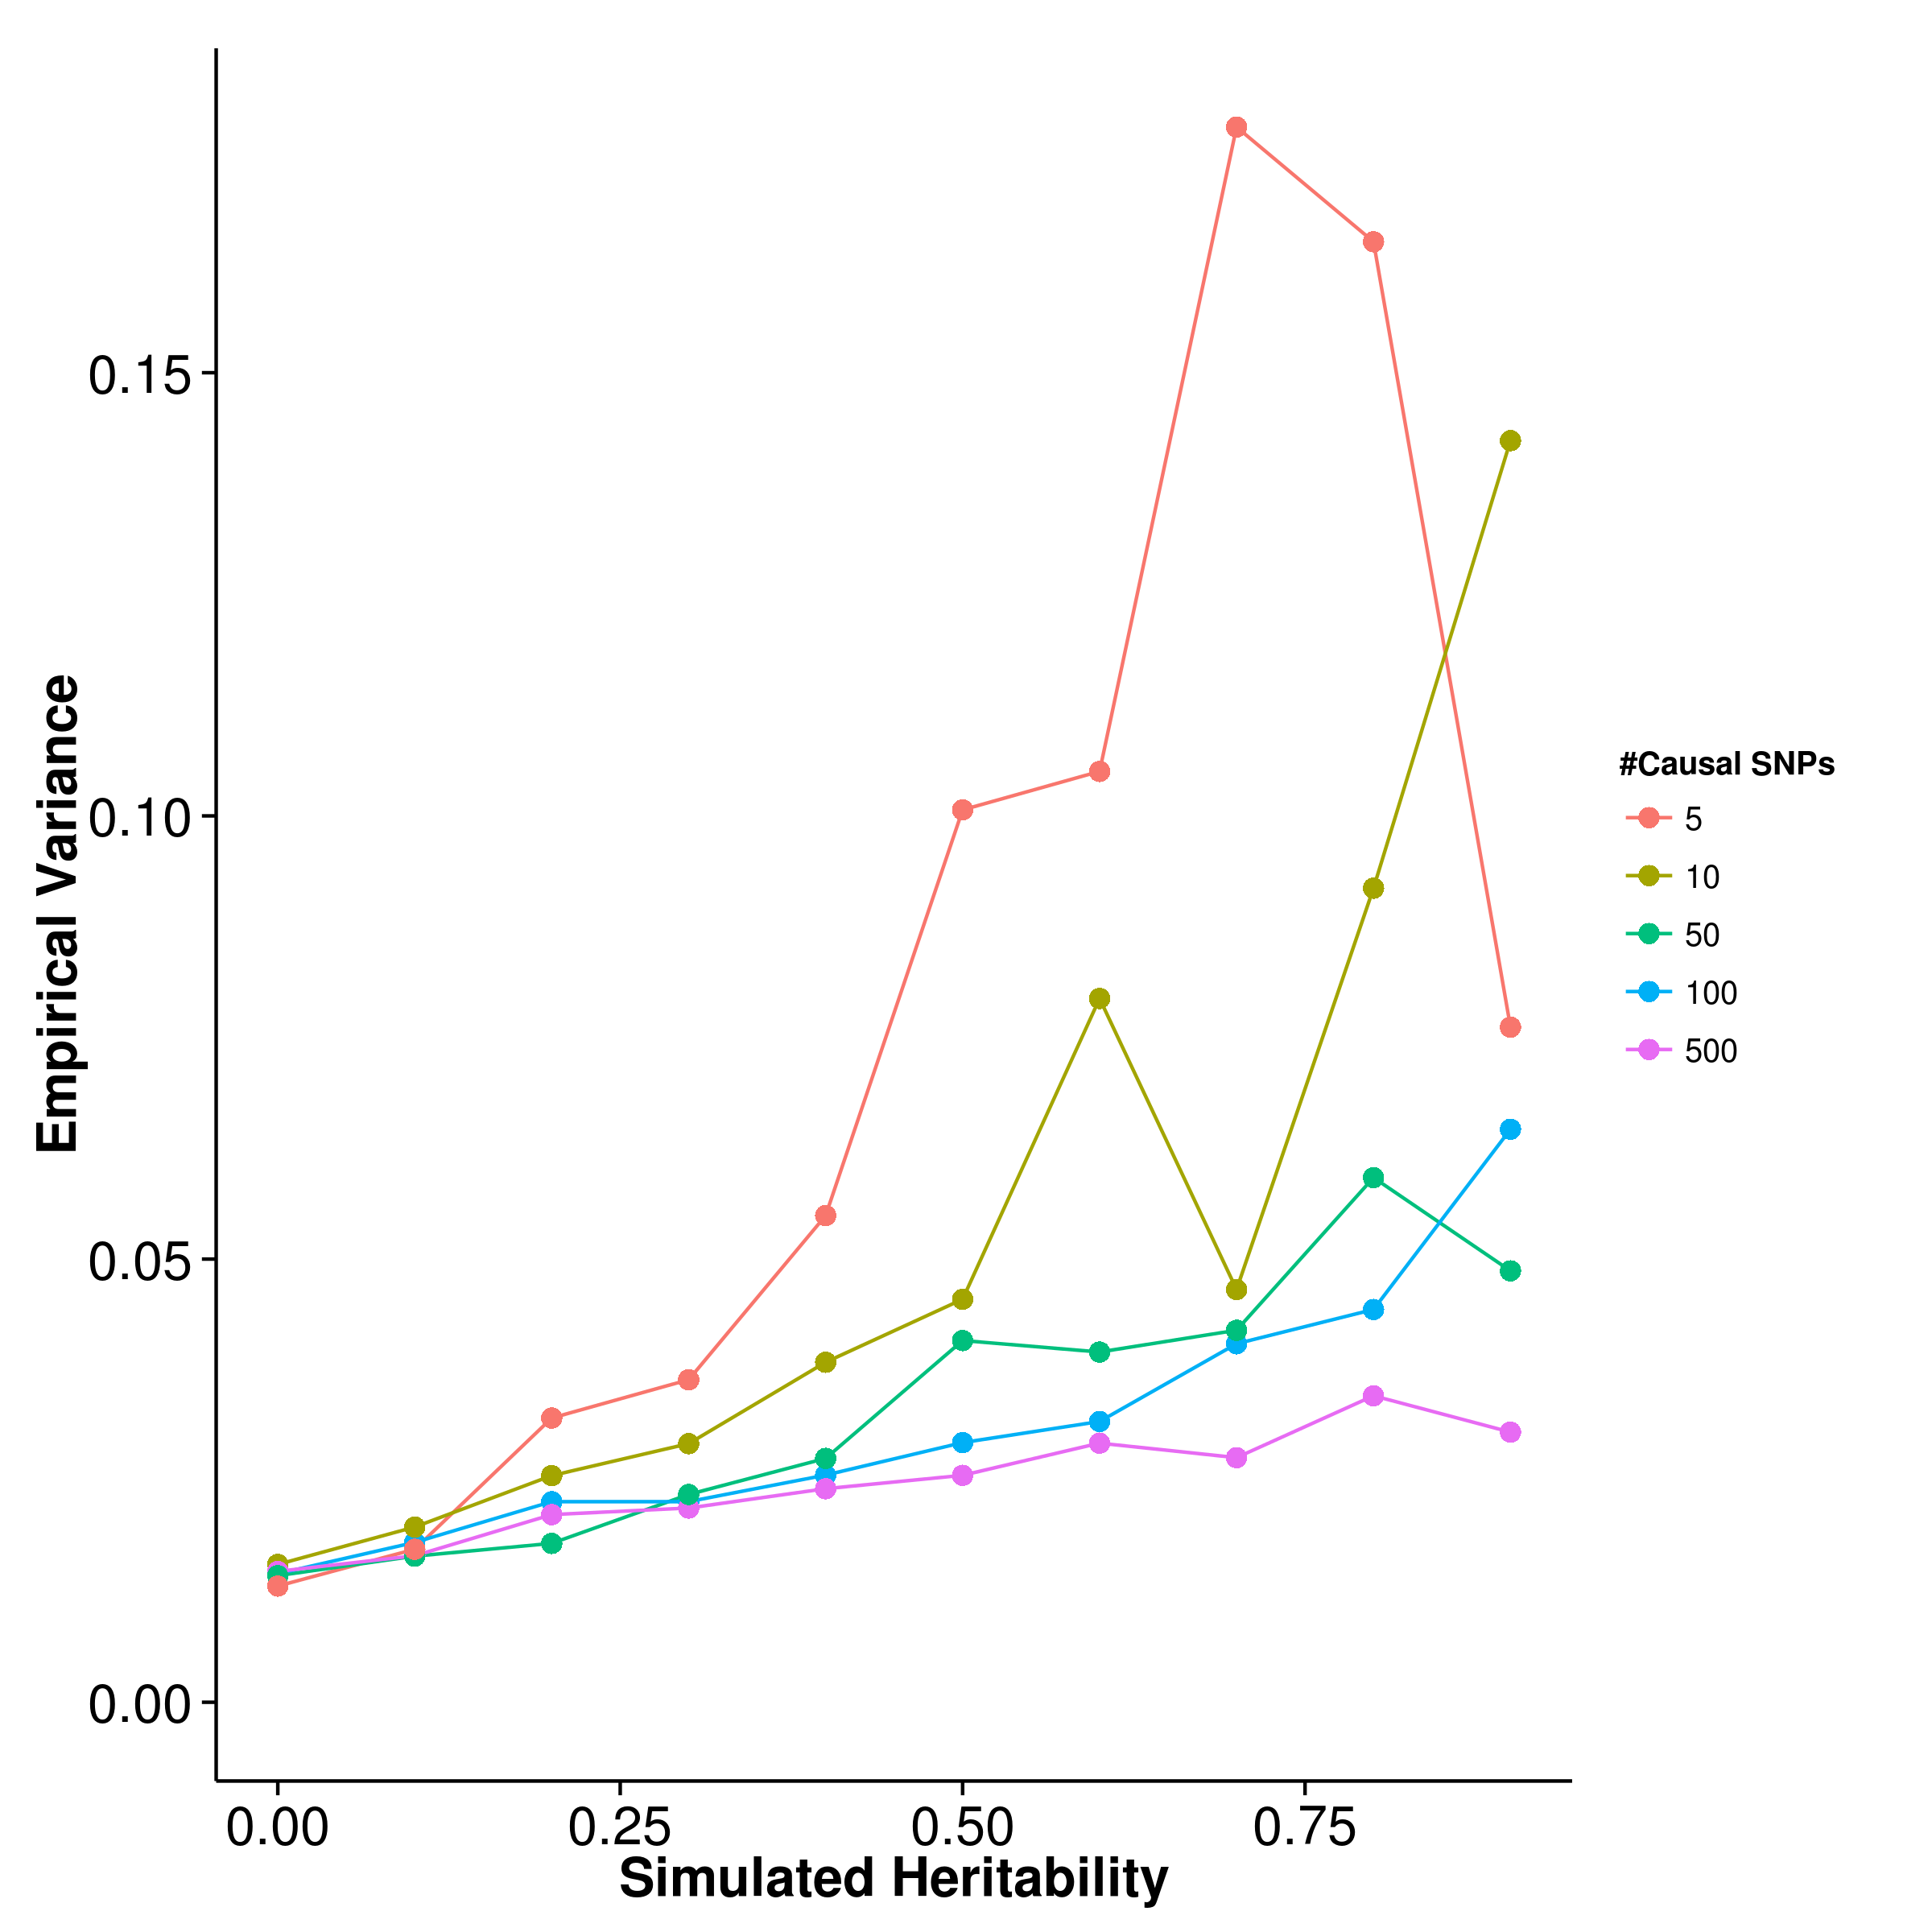
\includegraphics{figure/he_summary/random/ldscIn_Qt_Rand_sd.png}}
				\label{fig:ldscInQtRandVar}
			}
			\caption[Variance of Quantitative Trait Simulation Results]
			{Variance of results from quantitative trait simulation with random effect size simulation.
				Under the polygenic conditions, \gls{gcta} has the smallest variance, follow by \gls{ldsc}. 
				However, it was observed when the number of causal \glspl{SNP} decreases, the variance of the estimation increases for all algorithm, with variance of the \gls{shrek} estimate being the least affected.
				In fact, under oligogenic conditions, \gls{shrek} has a lower empirical variance when compared to \gls{ldsc}.
			} 
			\label{fig:QtRandVar}
		\end{figure}
		
		\begin{figure}
			\centering
			\subfloat[SHREK]{
				\scalebox{.4}{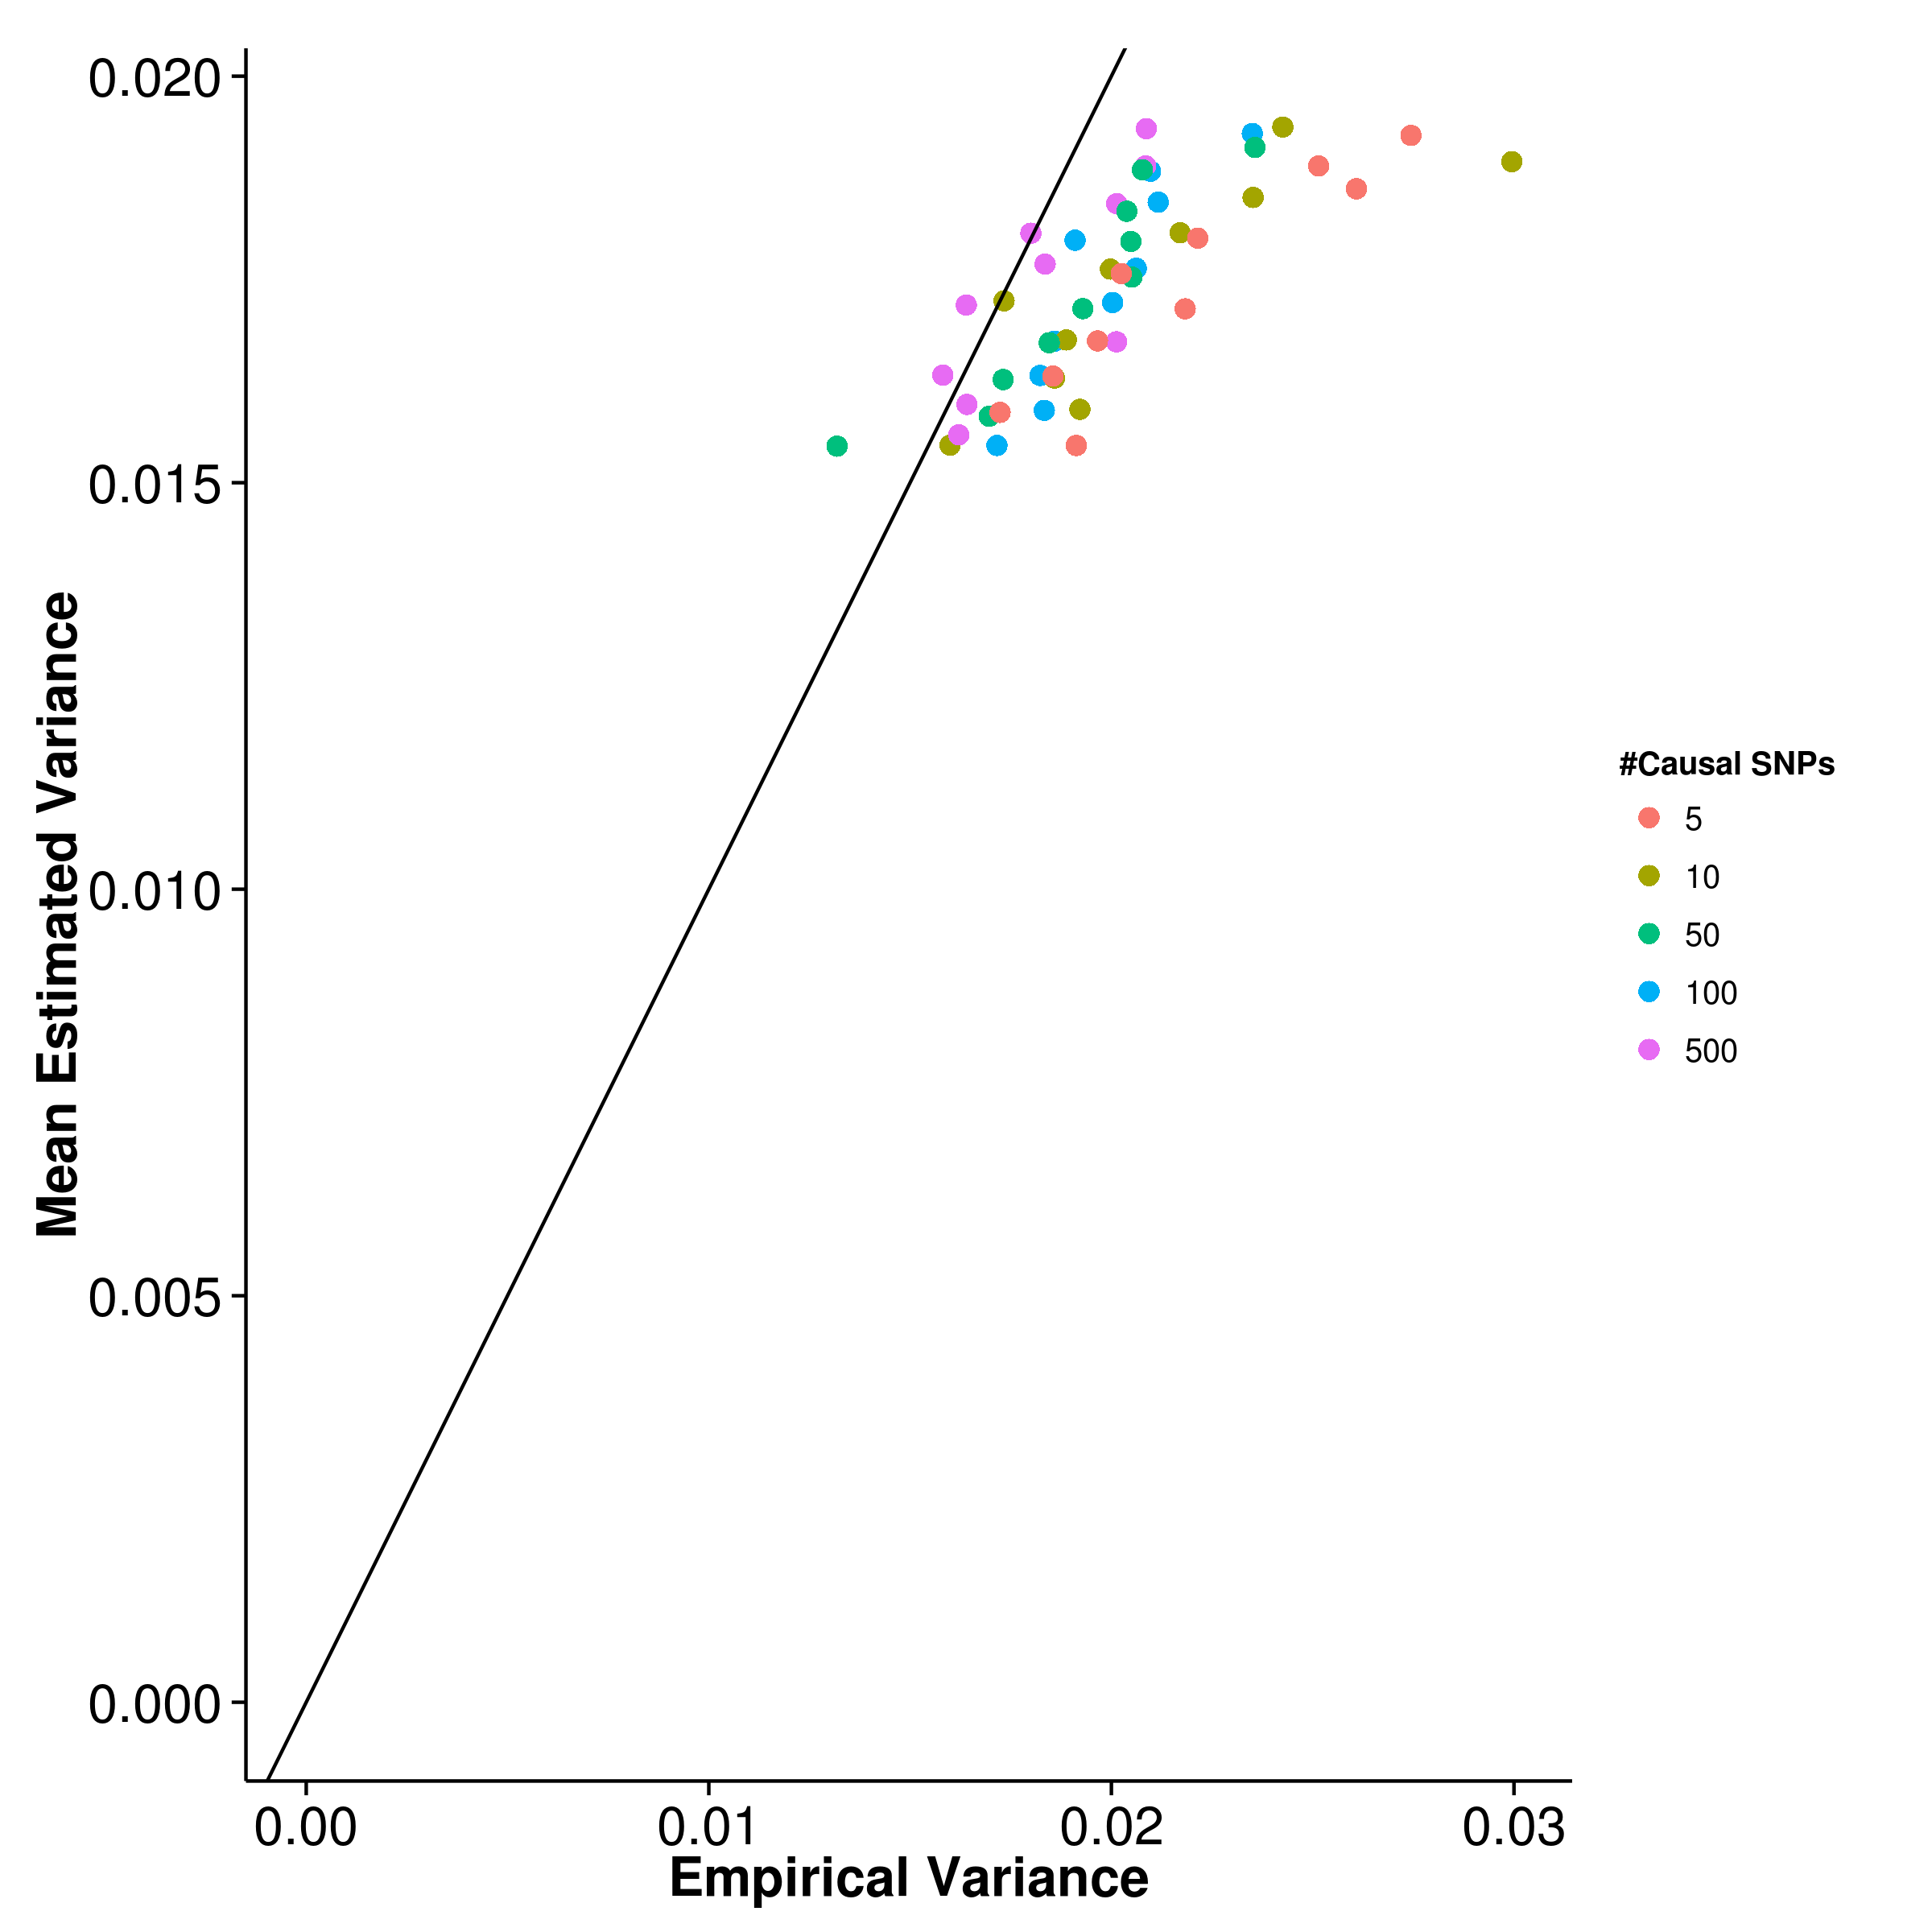
\includegraphics{figure/he_summary/random/shrek_Qt_Rand_sdCom.png}}
				\label{fig:shrekQtRandVarCom}
			}
			\subfloat[GCTA]{
				\scalebox{.4}{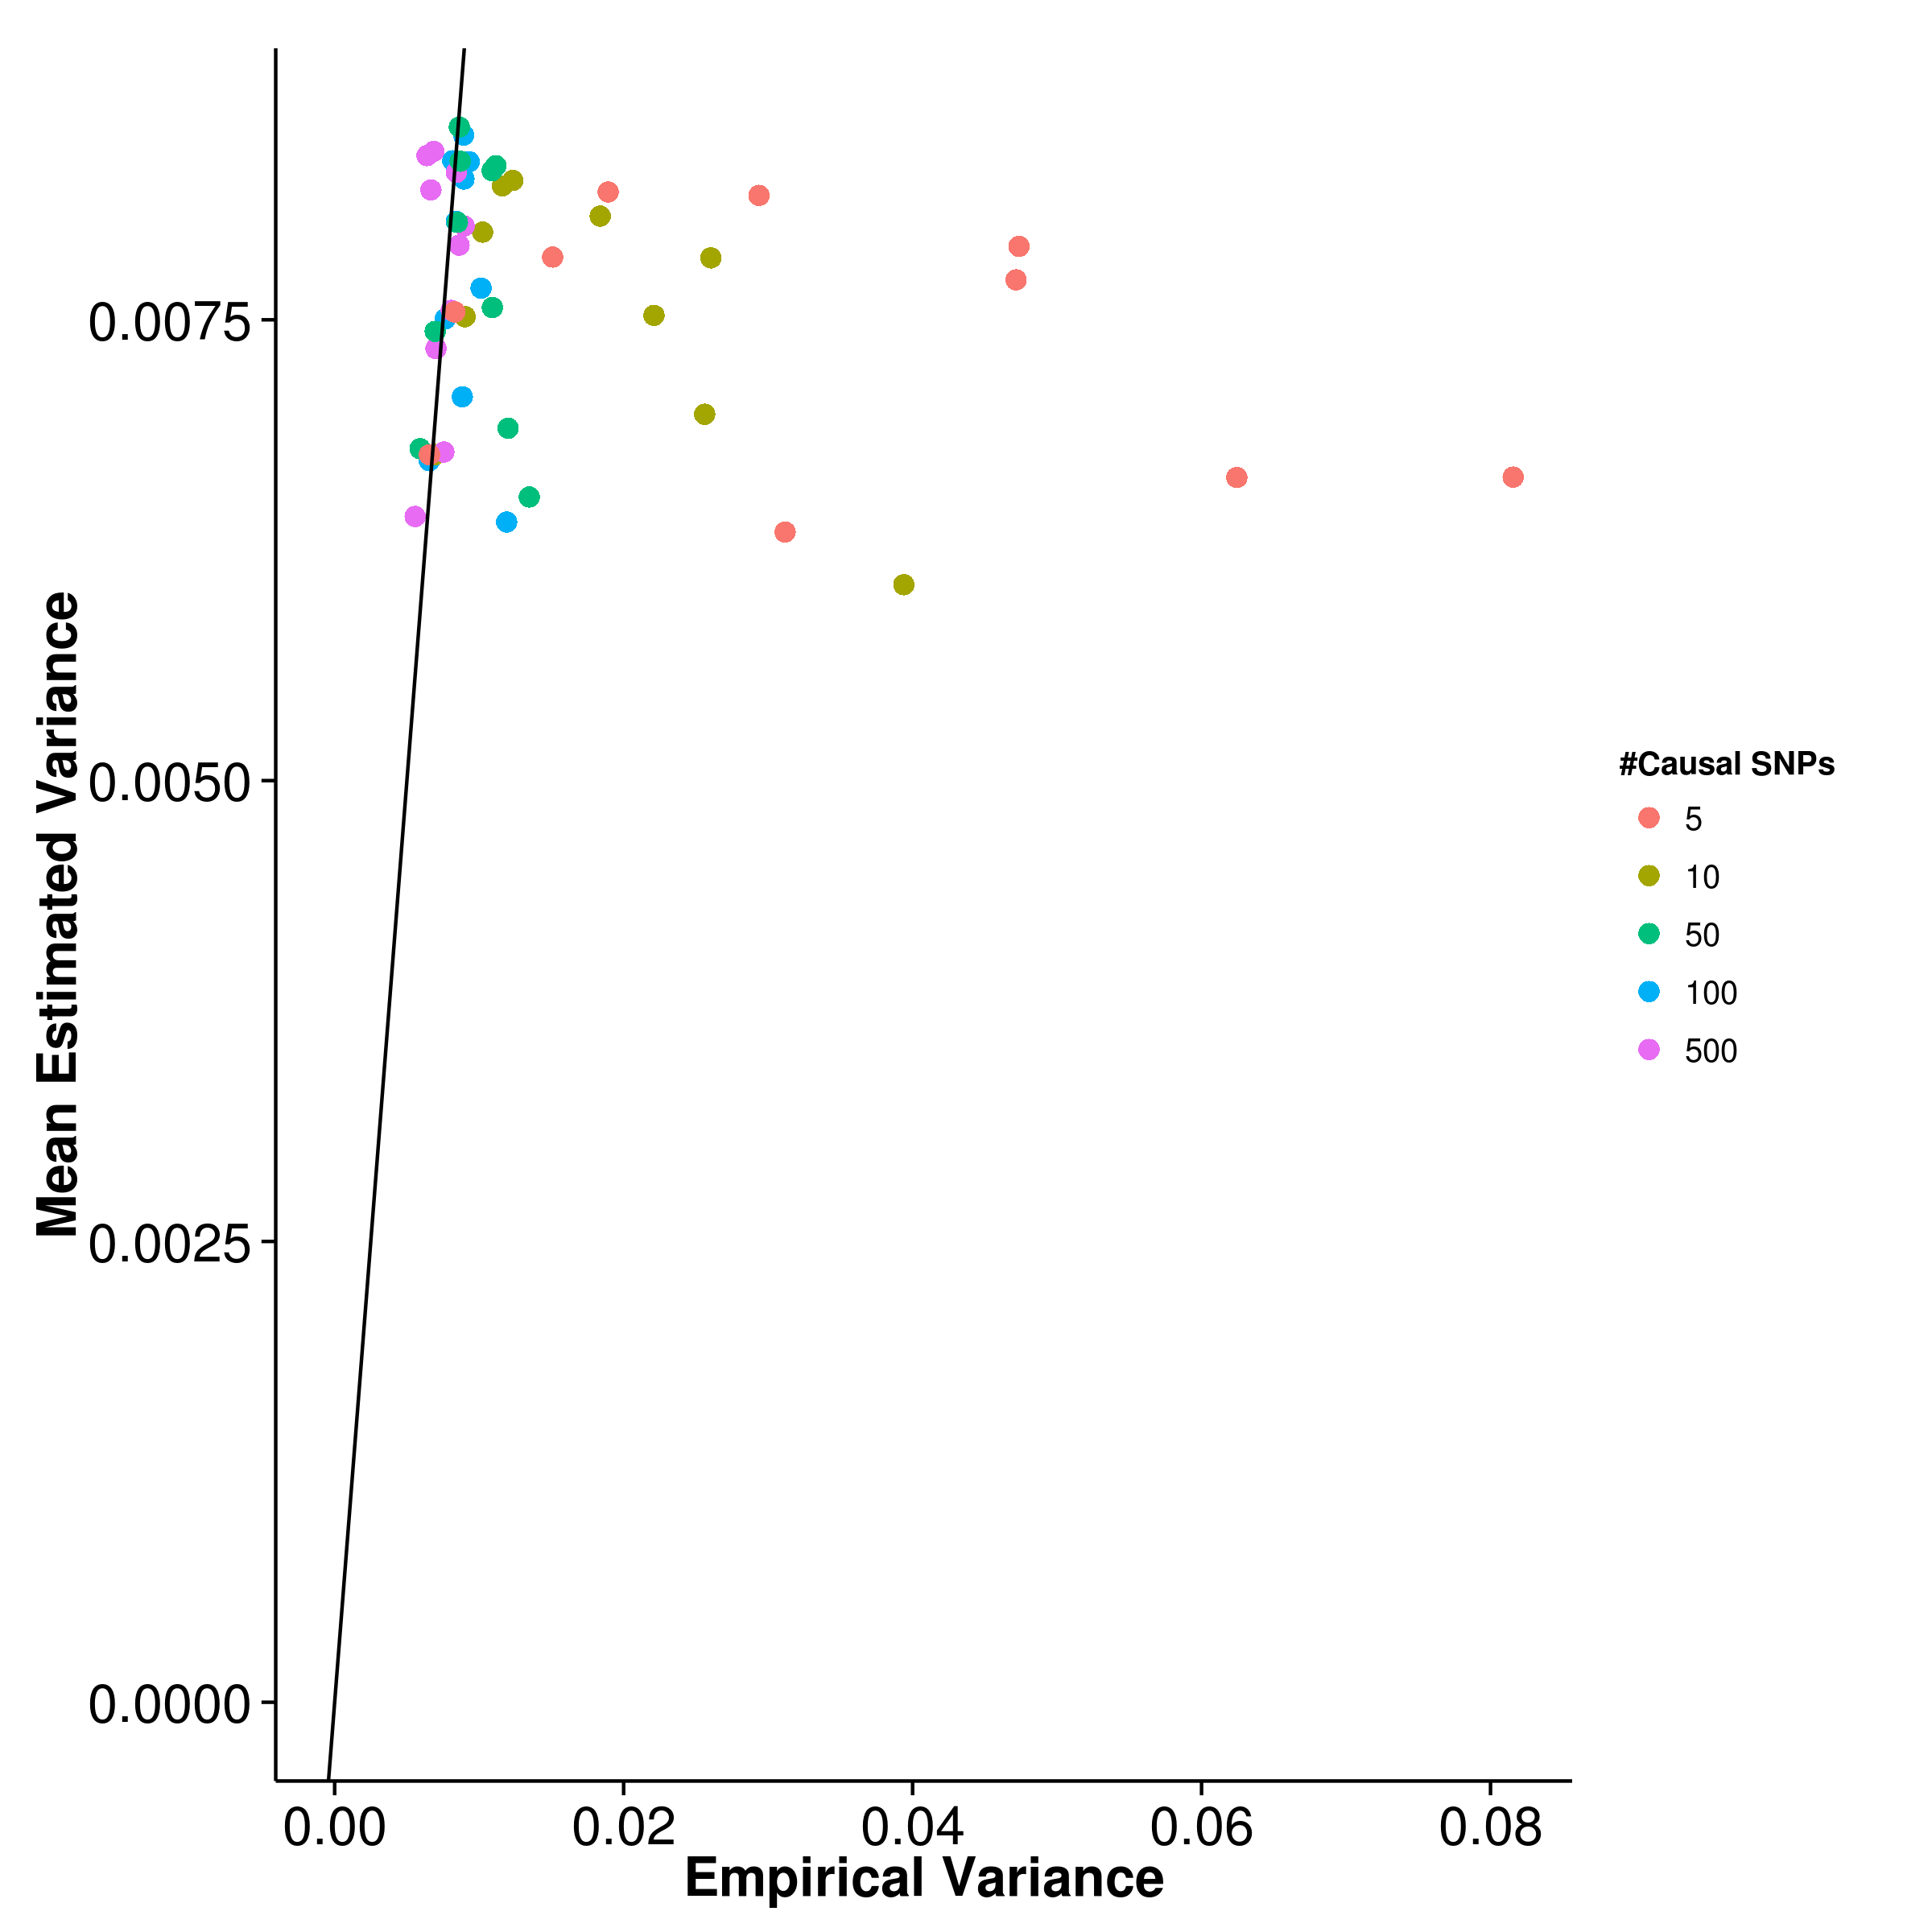
\includegraphics{figure/he_summary/random/gcta_Qt_Rand_sdCom.png}}
				\label{fig:gctaQtRandVarCom}
			}\\
			\subfloat[LDSC with fix intercept]{
				\scalebox{.4}{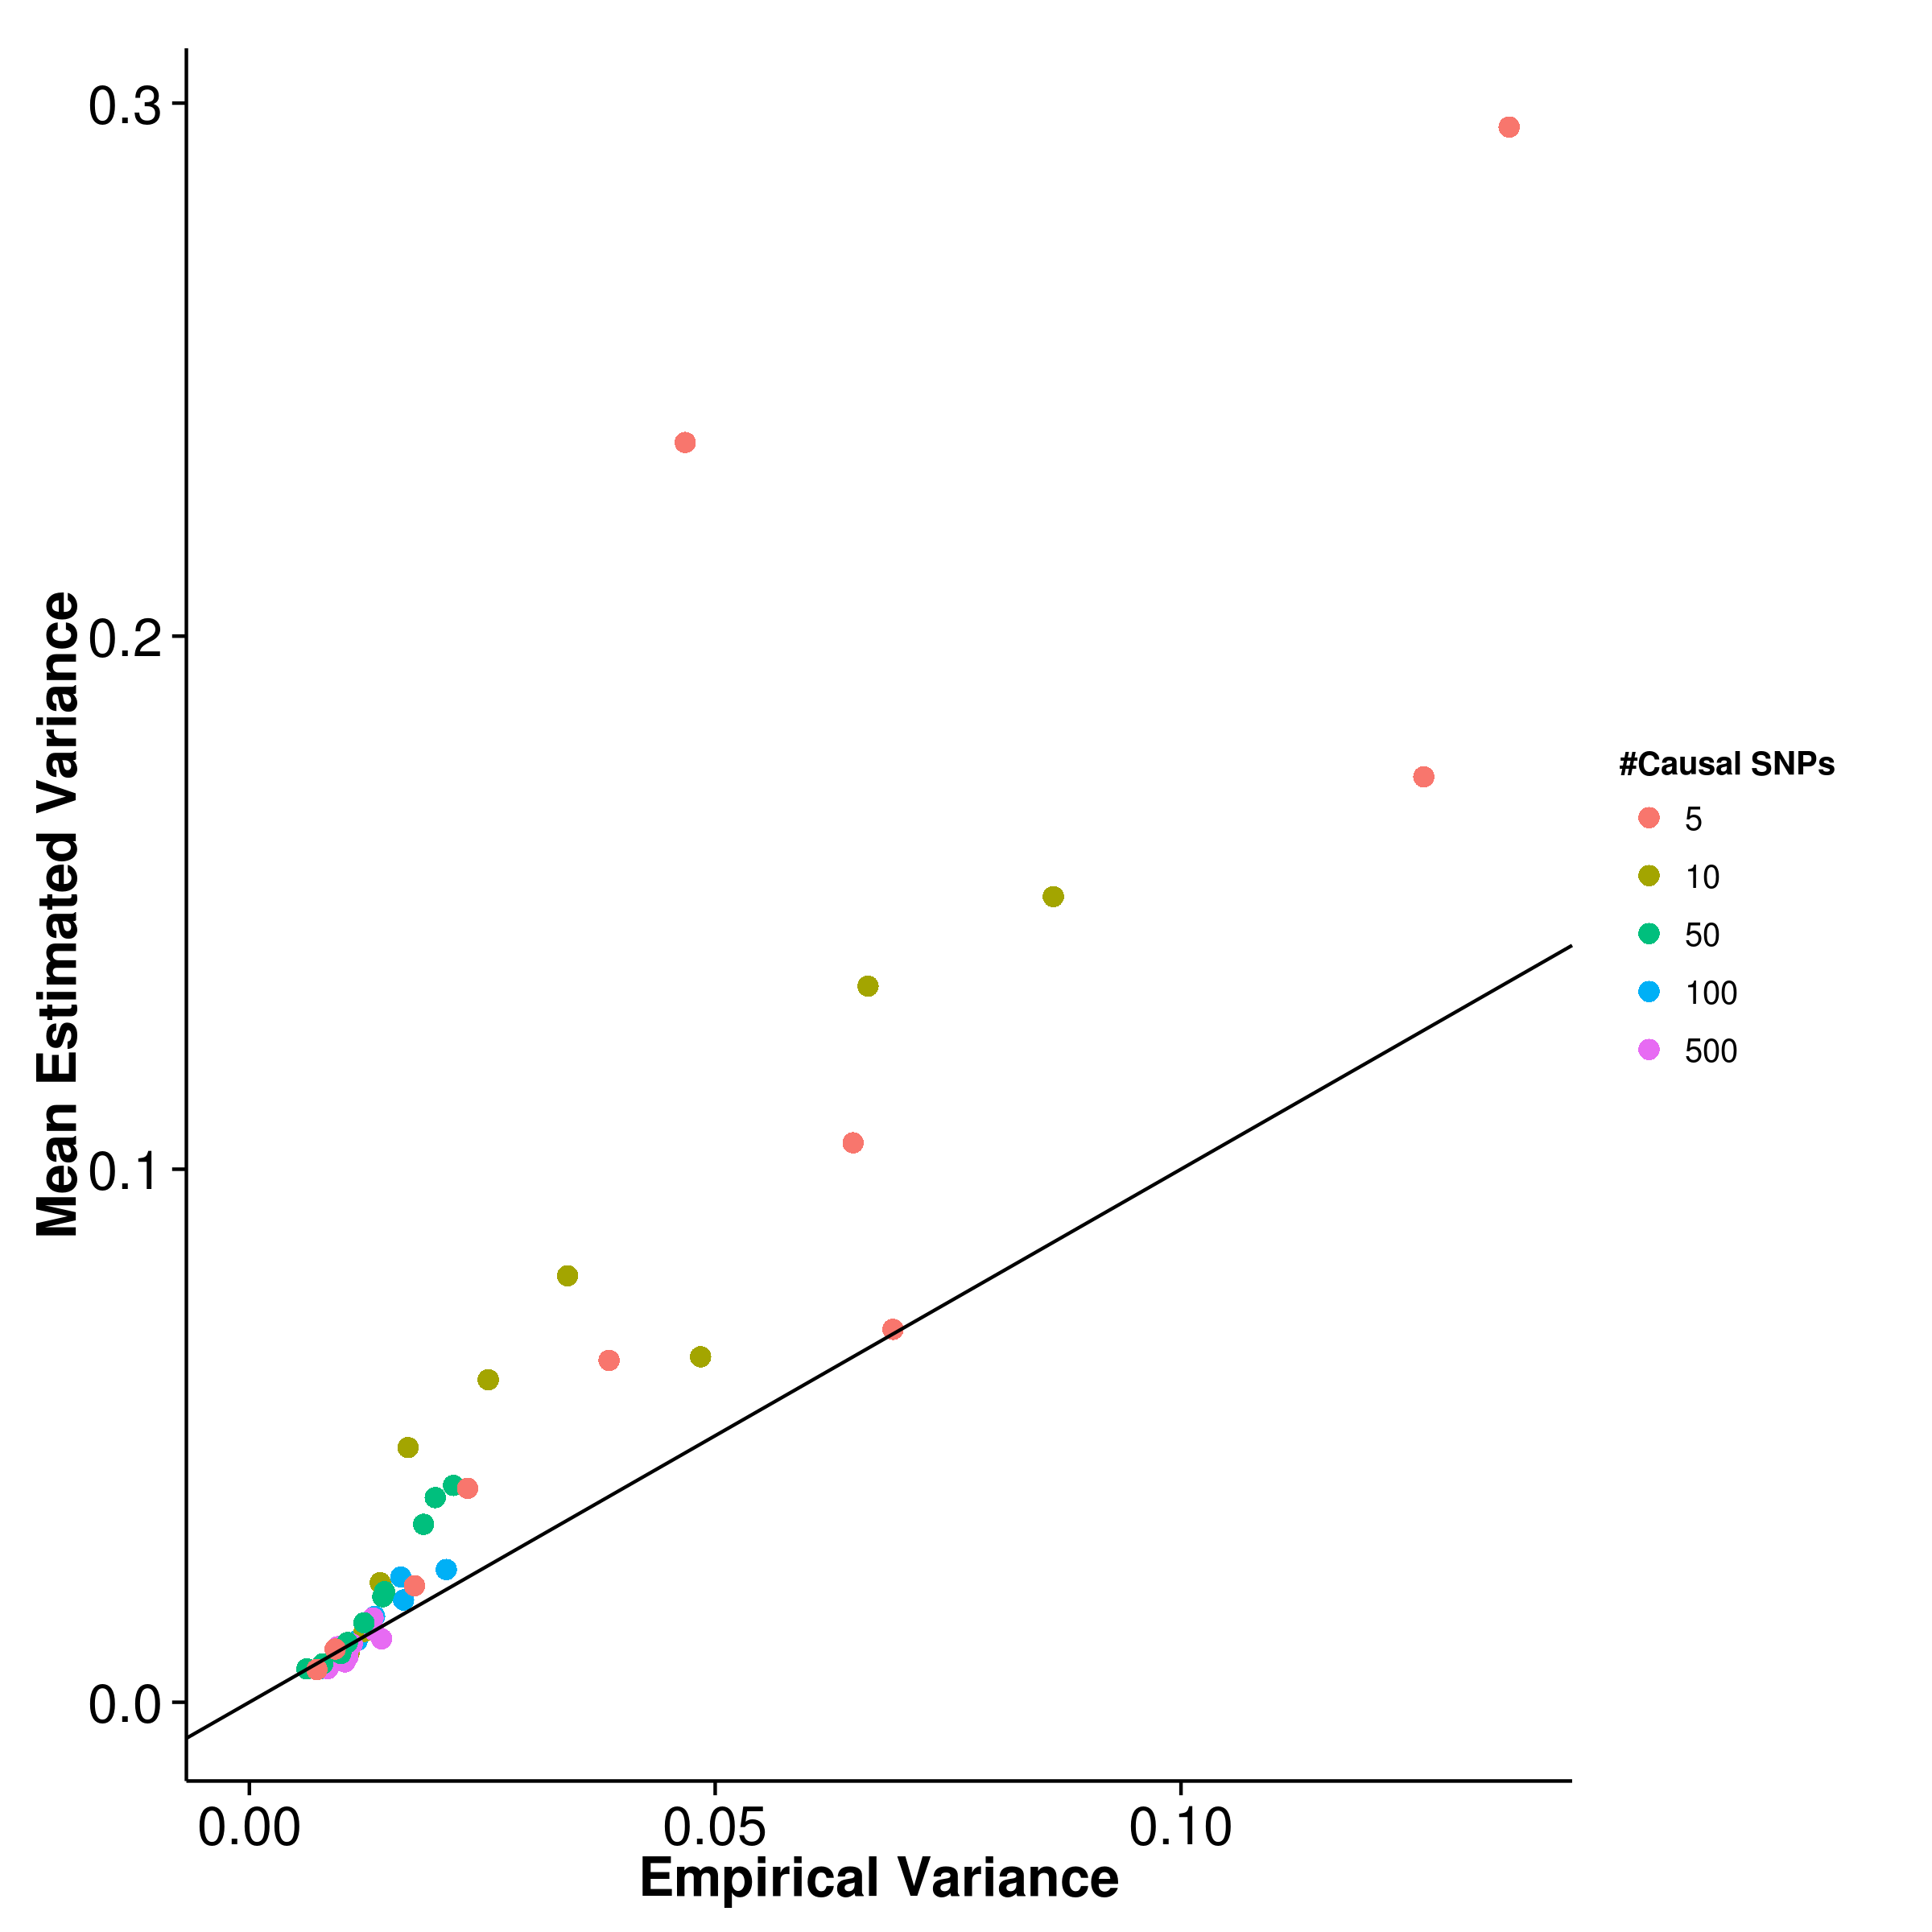
\includegraphics{figure/he_summary/random/ldsc_Qt_Rand_sdCom.png}}
				\label{fig:ldscQtRandVarCom}
			}
			\subfloat[LDSC with intercept estimation]{
				
				\scalebox{.4}{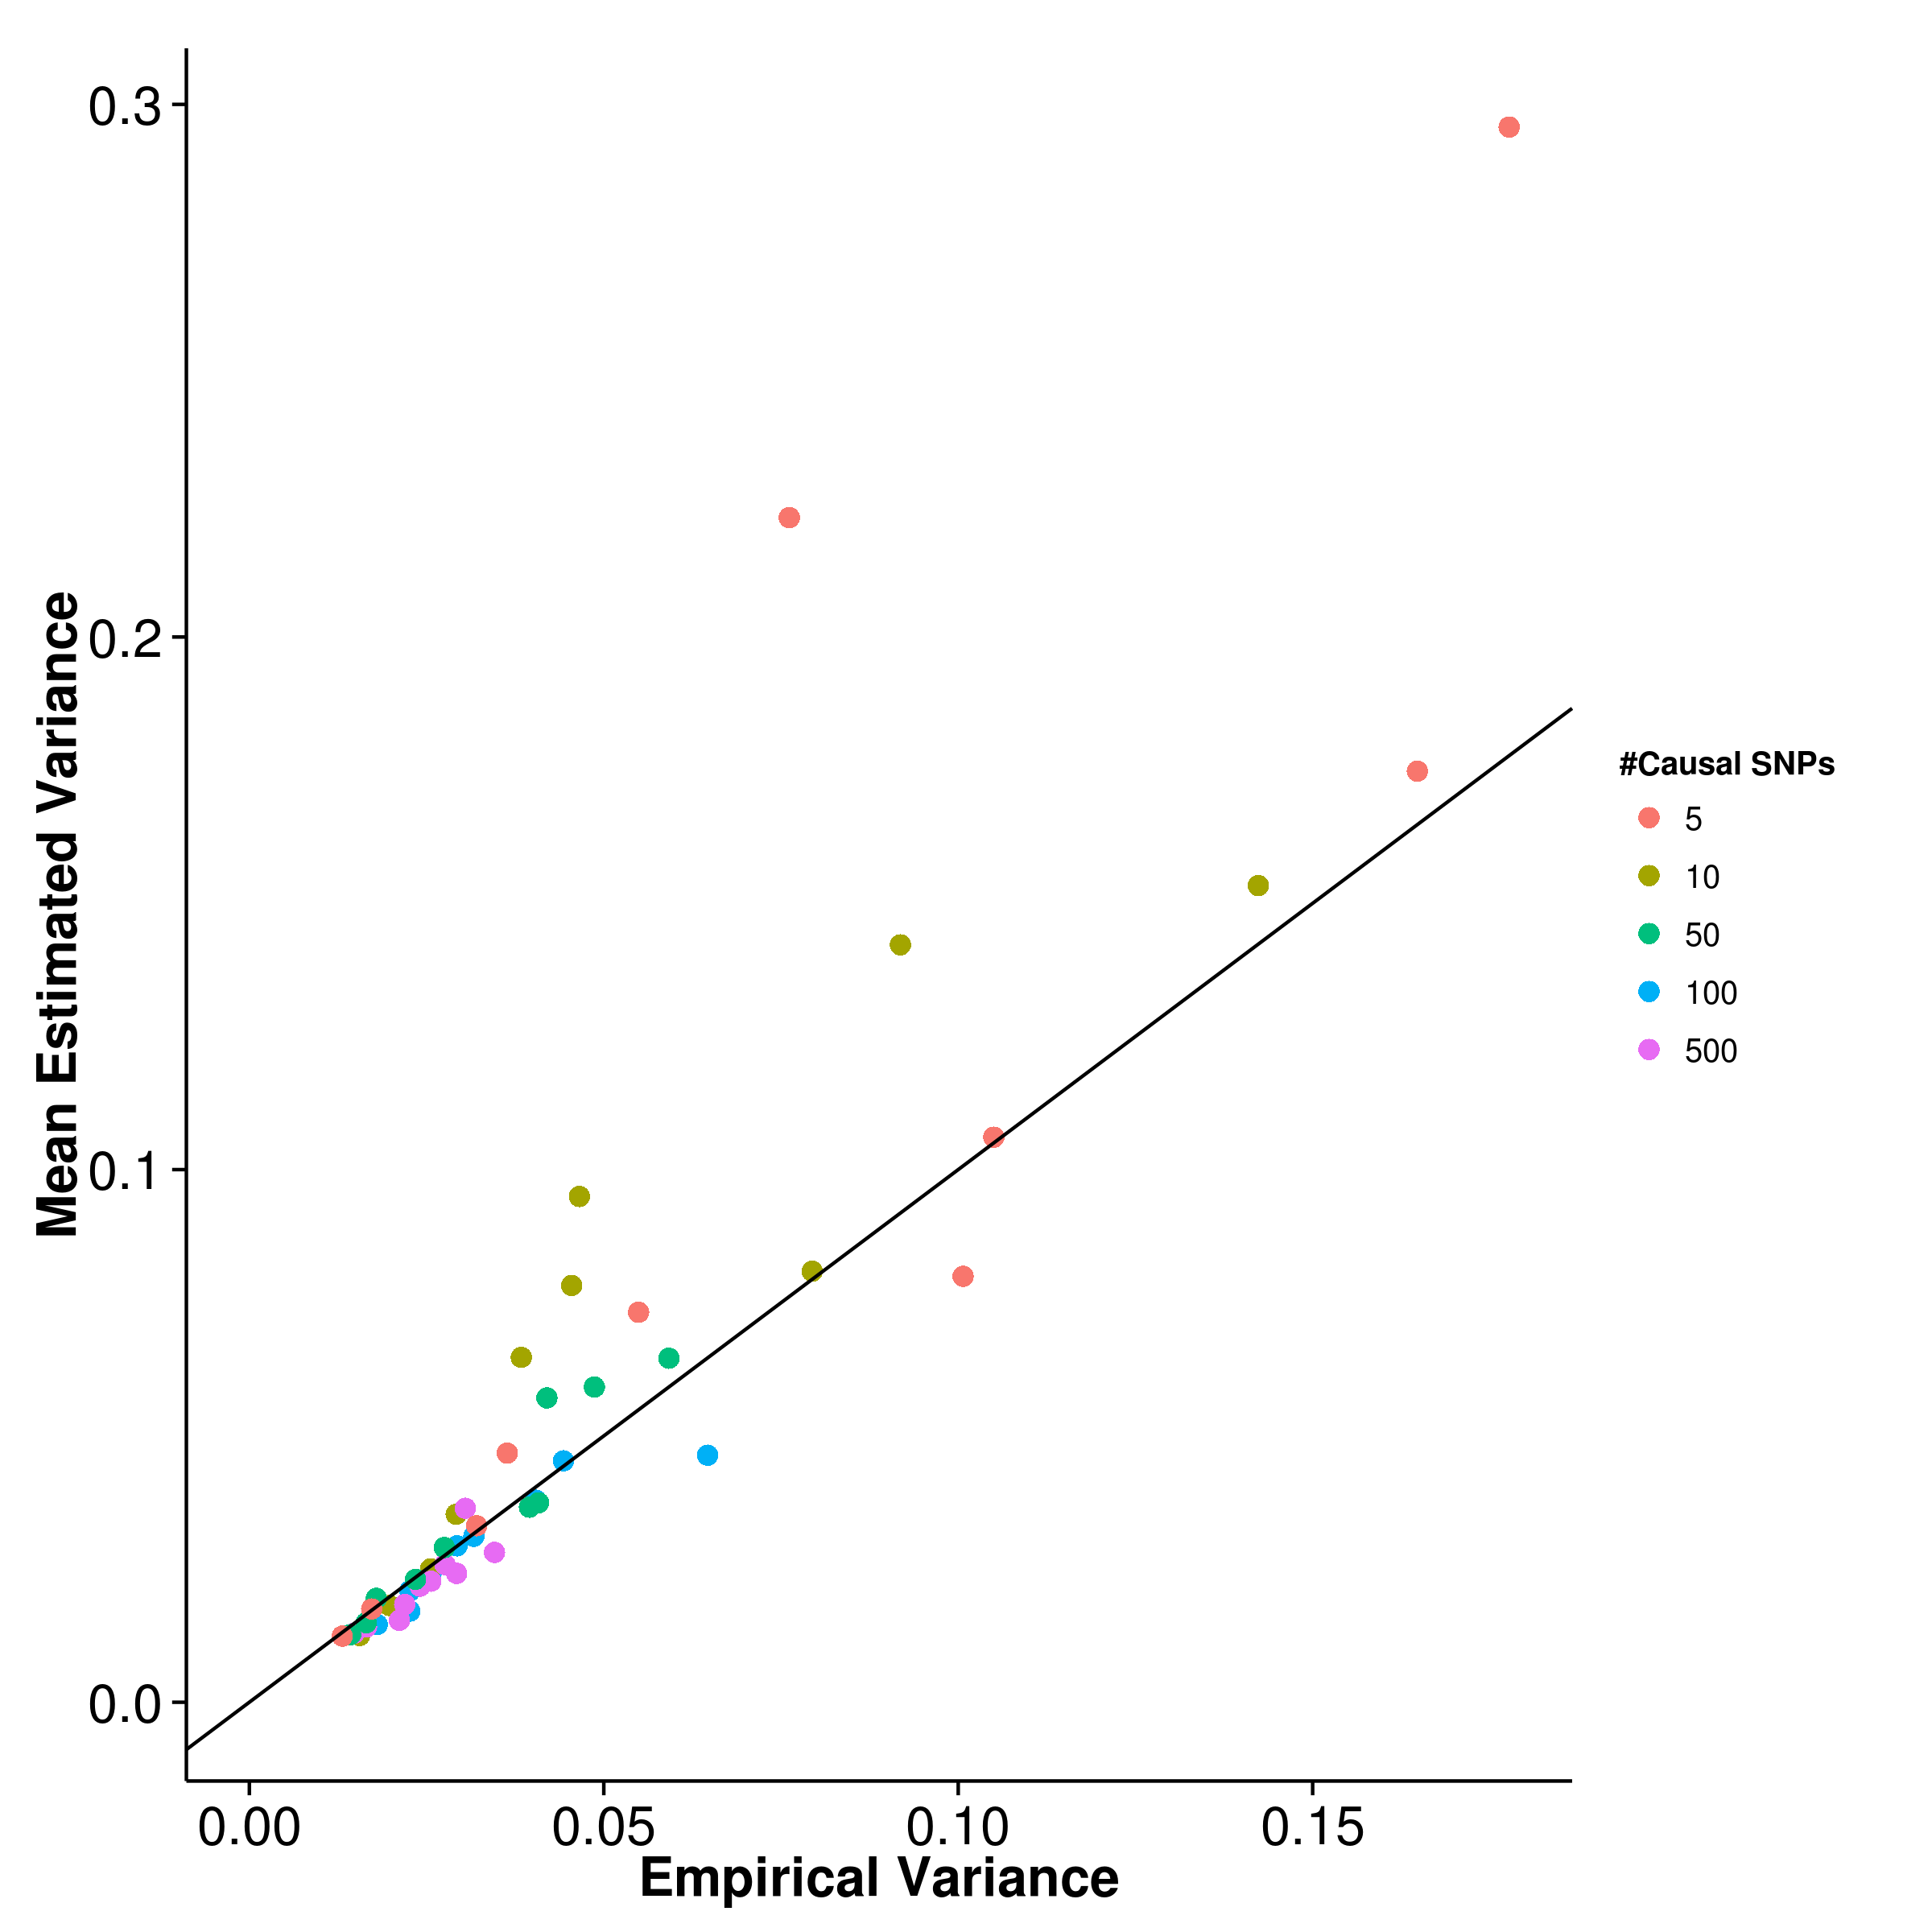
\includegraphics{figure/he_summary/random/ldscIn_Qt_Rand_sdCom.png}}
				\label{fig:ldscInQtRandVarCom}
			}
			\caption[Estimation of Variance in Quantitative Trait Simulation]
			{Estimated variance of results from quantitative trait simulation with random effect size simulation when compared to the empirical variance.
			\gls{gcta} has the best estimate of its empirical variance under the polygenic conditions whereas \gls{shrek} tends to under-estimate its empirical variance.
			On the other hand, \gls{ldsc} to over-estimate the variance especially when the number of causal \glspl{SNP} is small.
				} 
			\label{fig:QtRandVarCom}
		\end{figure}
		Next, we simulate quantitative trait with random effect size assigned to the causal \glspl{SNP}.
		The exponential distribution with $\lambda=1$ was selected because it was suggested that it may serve as a heuristic expectation the genetic architecture of adaptation\citep{Orr1998}.
		There might be many other distribution that can be used, however due to limitation in resources, we will only focus on the exponential distribution with $\lambda=1$.

		Under this simulation condition, it was observed that the mean estimation of heritability from \gls{shrek}(\cref{fig:shrekQtRandMean}) and \gls{gcta}(\cref{fig:gctaQtRandMean}) were similar to what was observed in the equal effect size simulation.
		For \gls{ldsc} with intercept estimation(\cref{fig:ldscInQtRandMean}), less bias was observed with only the 10 causal \glspl{SNP} scenario being under estimated. 
		On the other hand, the performance of \gls{ldsc} with fixed intercept remain more or less the same, with a larger degree of fluctuation when small number of causal \glspl{SNP}(5 or 10) was simulated. 
		The fluctuation in estimate can also be observed in the empirical variance of \gls{ldsc}(\cref{fig:ldscQtRandVar,fig:ldscInQtRandVar}).
		Despite the relative stable performance of \gls{gcta}, the empirical variance of \gls{gcta} also fluctuate when the number of causal \glspl{SNP} was small. 
		Such pattern was not observed in \gls{shrek} suggesting that it might be robust against the change in number of causal \glspl{SNP}.
		
		When inspecting the relationship between the estimated and empirical variance, it was observed all programmes have a less accurate estimation of its variance when there is only 5 causal \glspl{SNP}. 
		The difference was most obvious for \gls{gcta} where the under-estimation of variance under the oligo-genic scenario(5 or 10 causal \glspl{SNP}) was more severe when a random effect size was assigned to the causal \glspl{SNP}(\cref{fig:gctaQtRandVarCom}).    
		On the other hand, the degree of bias in estimating the variance remain more or less unchanged for \gls{shrek}(\cref{fig:shrekQtRandVarCom}) and \gls{ldsc} with intercept estimation(\cref{fig:ldscInQtRandVarCom}), with roughly 0.9 and 1.25 times difference from the empirical variance respectively.
		However, for \gls{ldsc} with fixed intercept(\cref{fig:ldscQtRandVarCom}), the fold difference increased slightly, changed from 1.5 fold difference to 1.65 fold difference.
		
		Overall, simulating the effect size using the exponential distribution only slightly increases the \gls{mse} of the programmes when the number of causal \glspl{SNP} is small and decreases the \gls{mse} when the number of causal \glspl{SNP} is larger. 
		Taking into considering of both the bias and standard error, \gls{shrek} has the better performance over \gls{ldsc} except when the trait is extremely polygenic(e.g. $\ge500$ causal \glspl{SNP}).
		\begin{table}
			\centering
			\begin{tabular}{rrrrr}
				\toprule
				Number of Causal SNPs&	SHREK&	LDSC&	LDSC-In&	GCTA \\
				\midrule
				5	&	0.177	&	0.565	&	0.584	&	0.230\\
				10	&	0.159	&	0.251	&	0.470	&	0.151\\
				50	&	0.153	&	0.179	&	0.378	&	0.0796\\
				100	&	0.157	&	0.166	&	0.305	&	0.0794\\
				250	&	0.152	&	0.144	&	0.266	&	0.0674\\
				500	&	0.143	&	0.134	&	0.247	&	0.0646\\
				\bottomrule
			\end{tabular}
			\caption[Mean Squared Error of Quantitative Trait Simulation with Random Effect Size]{
				\gls{mse} of quantitative trait simulation with random effect size.
				Again, \gls{gcta} has the lowest \gls{mse} except when there is only 5 causal \glspl{SNP} and the performance of \gls{shrek} and \gls{ldsc} with fix intercept converges as number of causal \glspl{SNP} increases. 
				\gls{ldsc} with fix intercept even surpassed \gls{shrek}'s performance when the number of causal \glspl{SNP} was as high as 500.}
			\label{tab:mseQtRandom}
		\end{table}
		% Extreme with 100 causal
		\subsection{Quantitative Trait Simulation with Extreme Effect Size}
		
		\begin{figure}
			\centering
			\subfloat[SHREK]{
				\scalebox{.4}{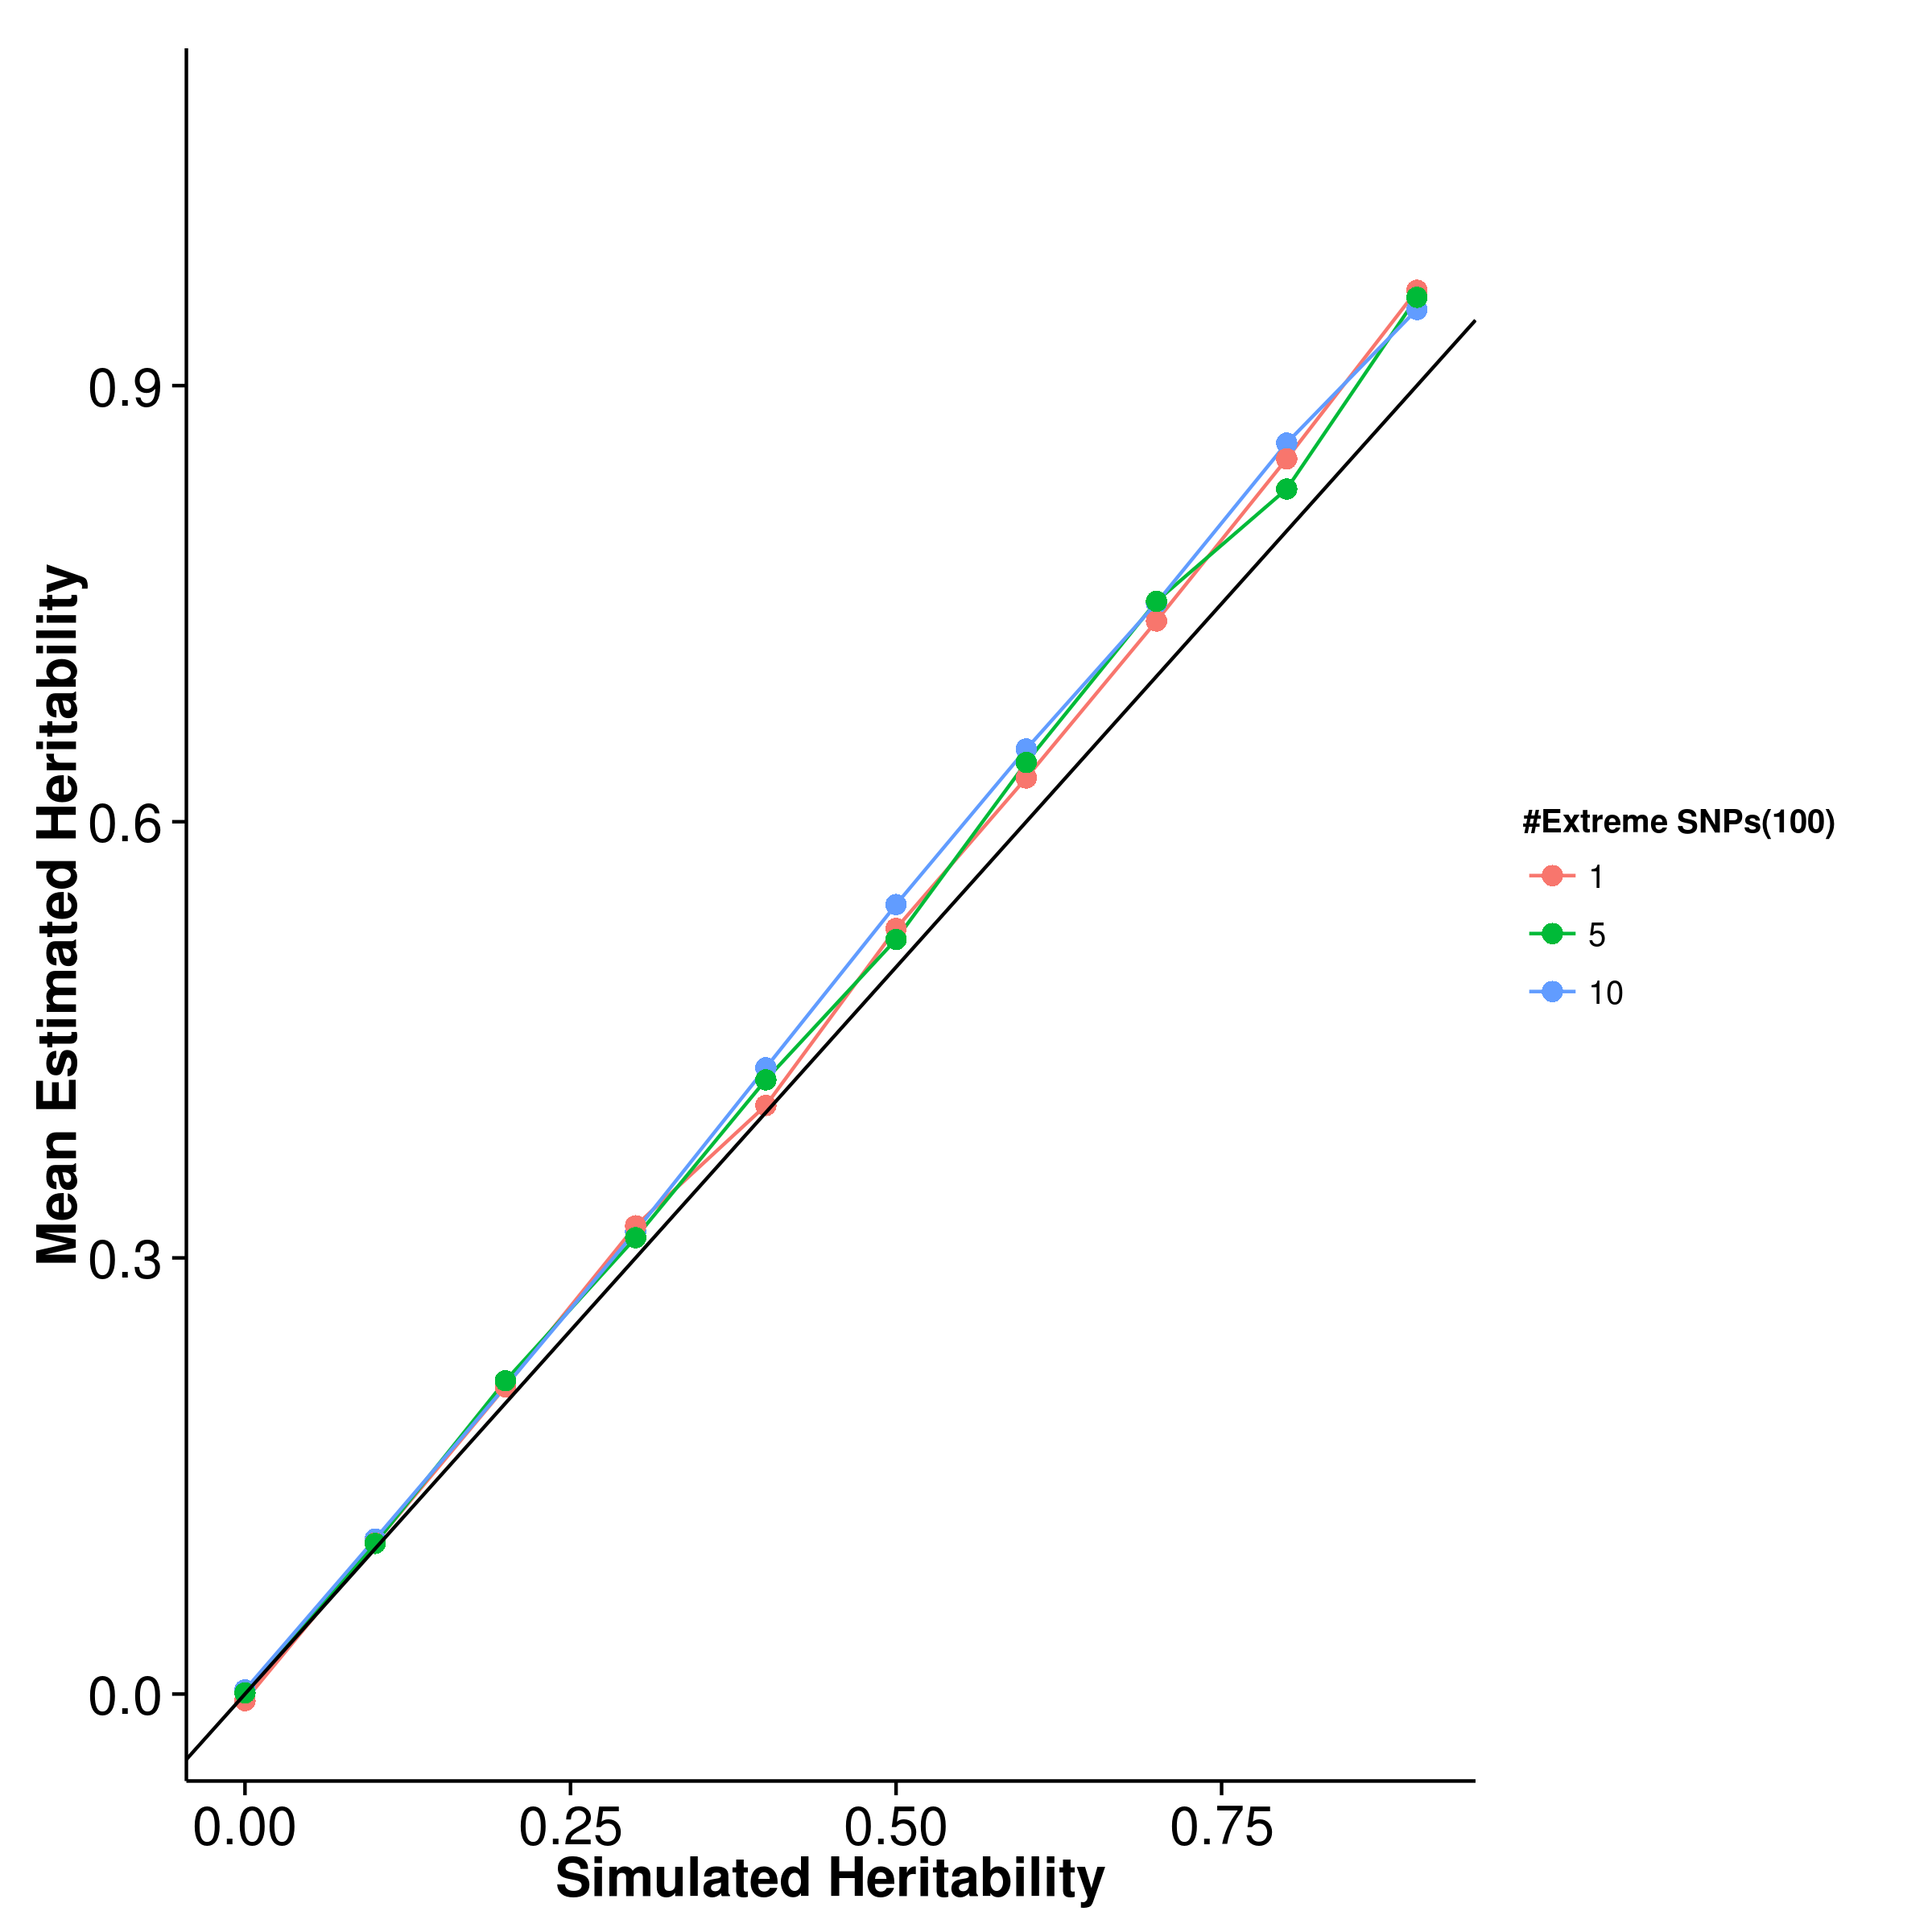
\includegraphics{figure/he_summary/extreme_100c/shrek_QtE_Rand_mean.png}}
				\label{fig:shrekQtEx100cMean}
			}
			\subfloat[GCTA]{
				\scalebox{.4}{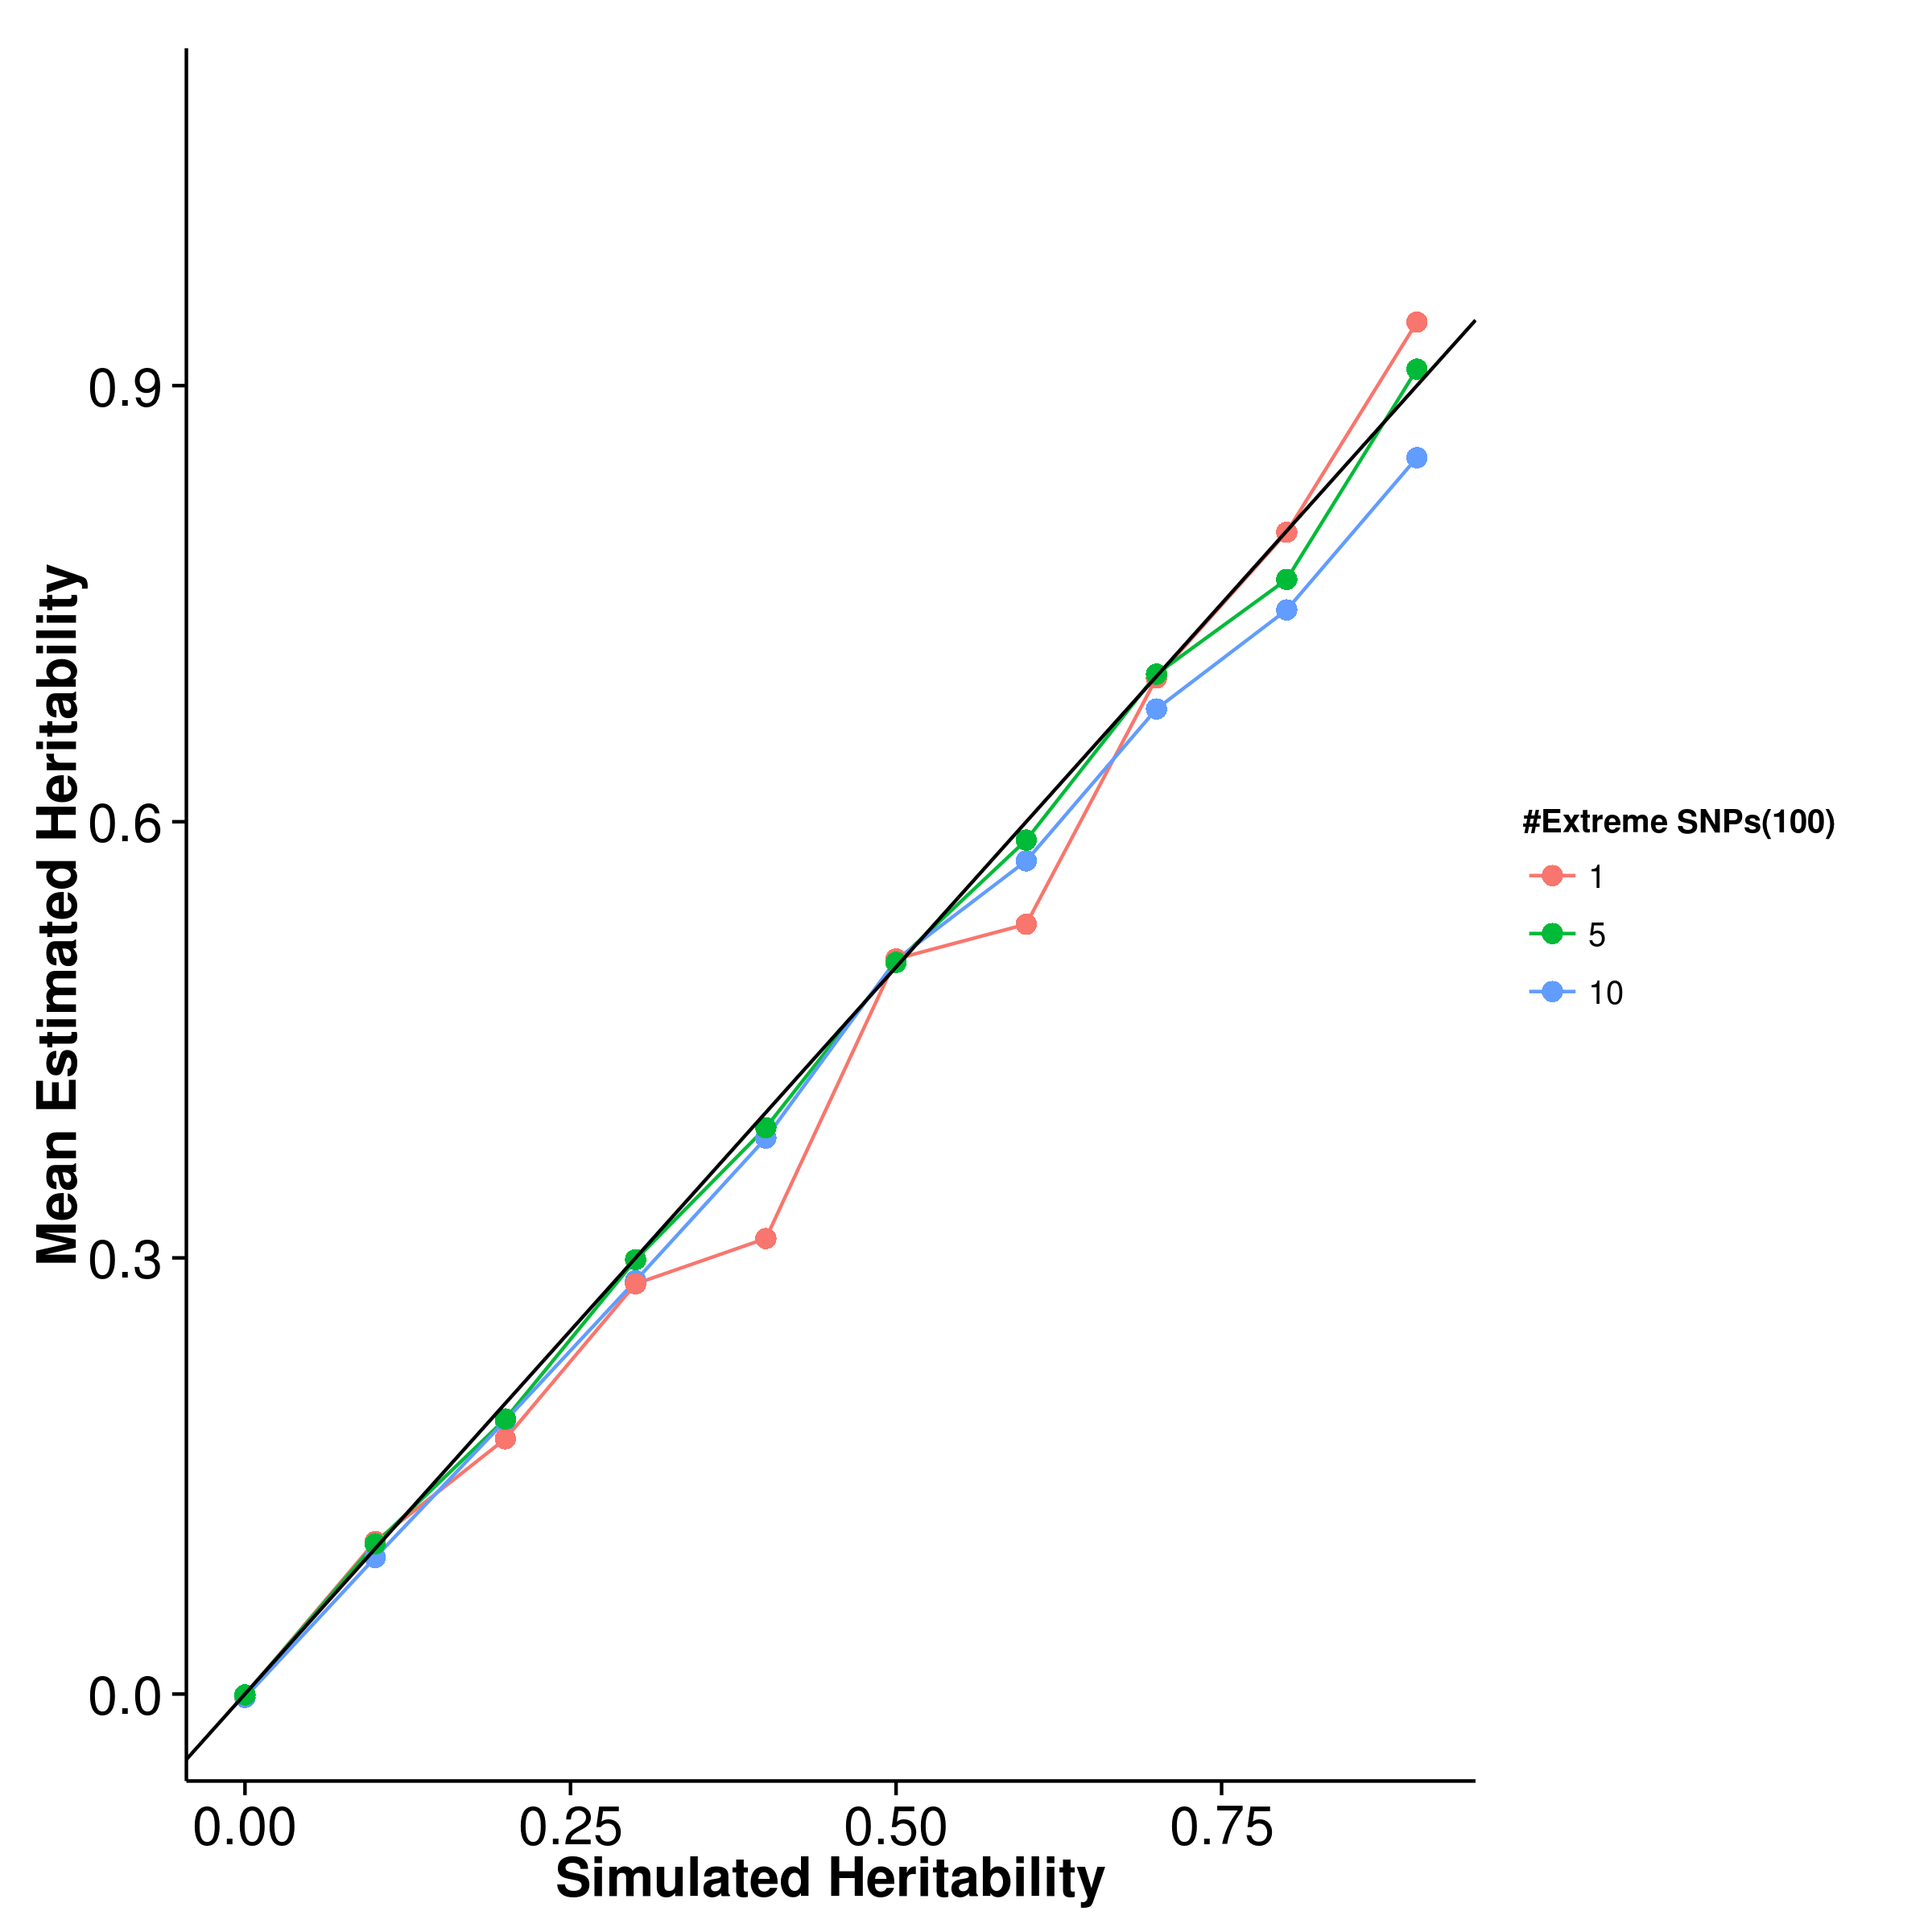
\includegraphics{figure/he_summary/extreme_100c/gcta_QtE_Rand_mean.png}}
				\label{fig:gctaQtEx100cMean}
			}\\
			\subfloat[LDSC with fix intercept]{
				\scalebox{.4}{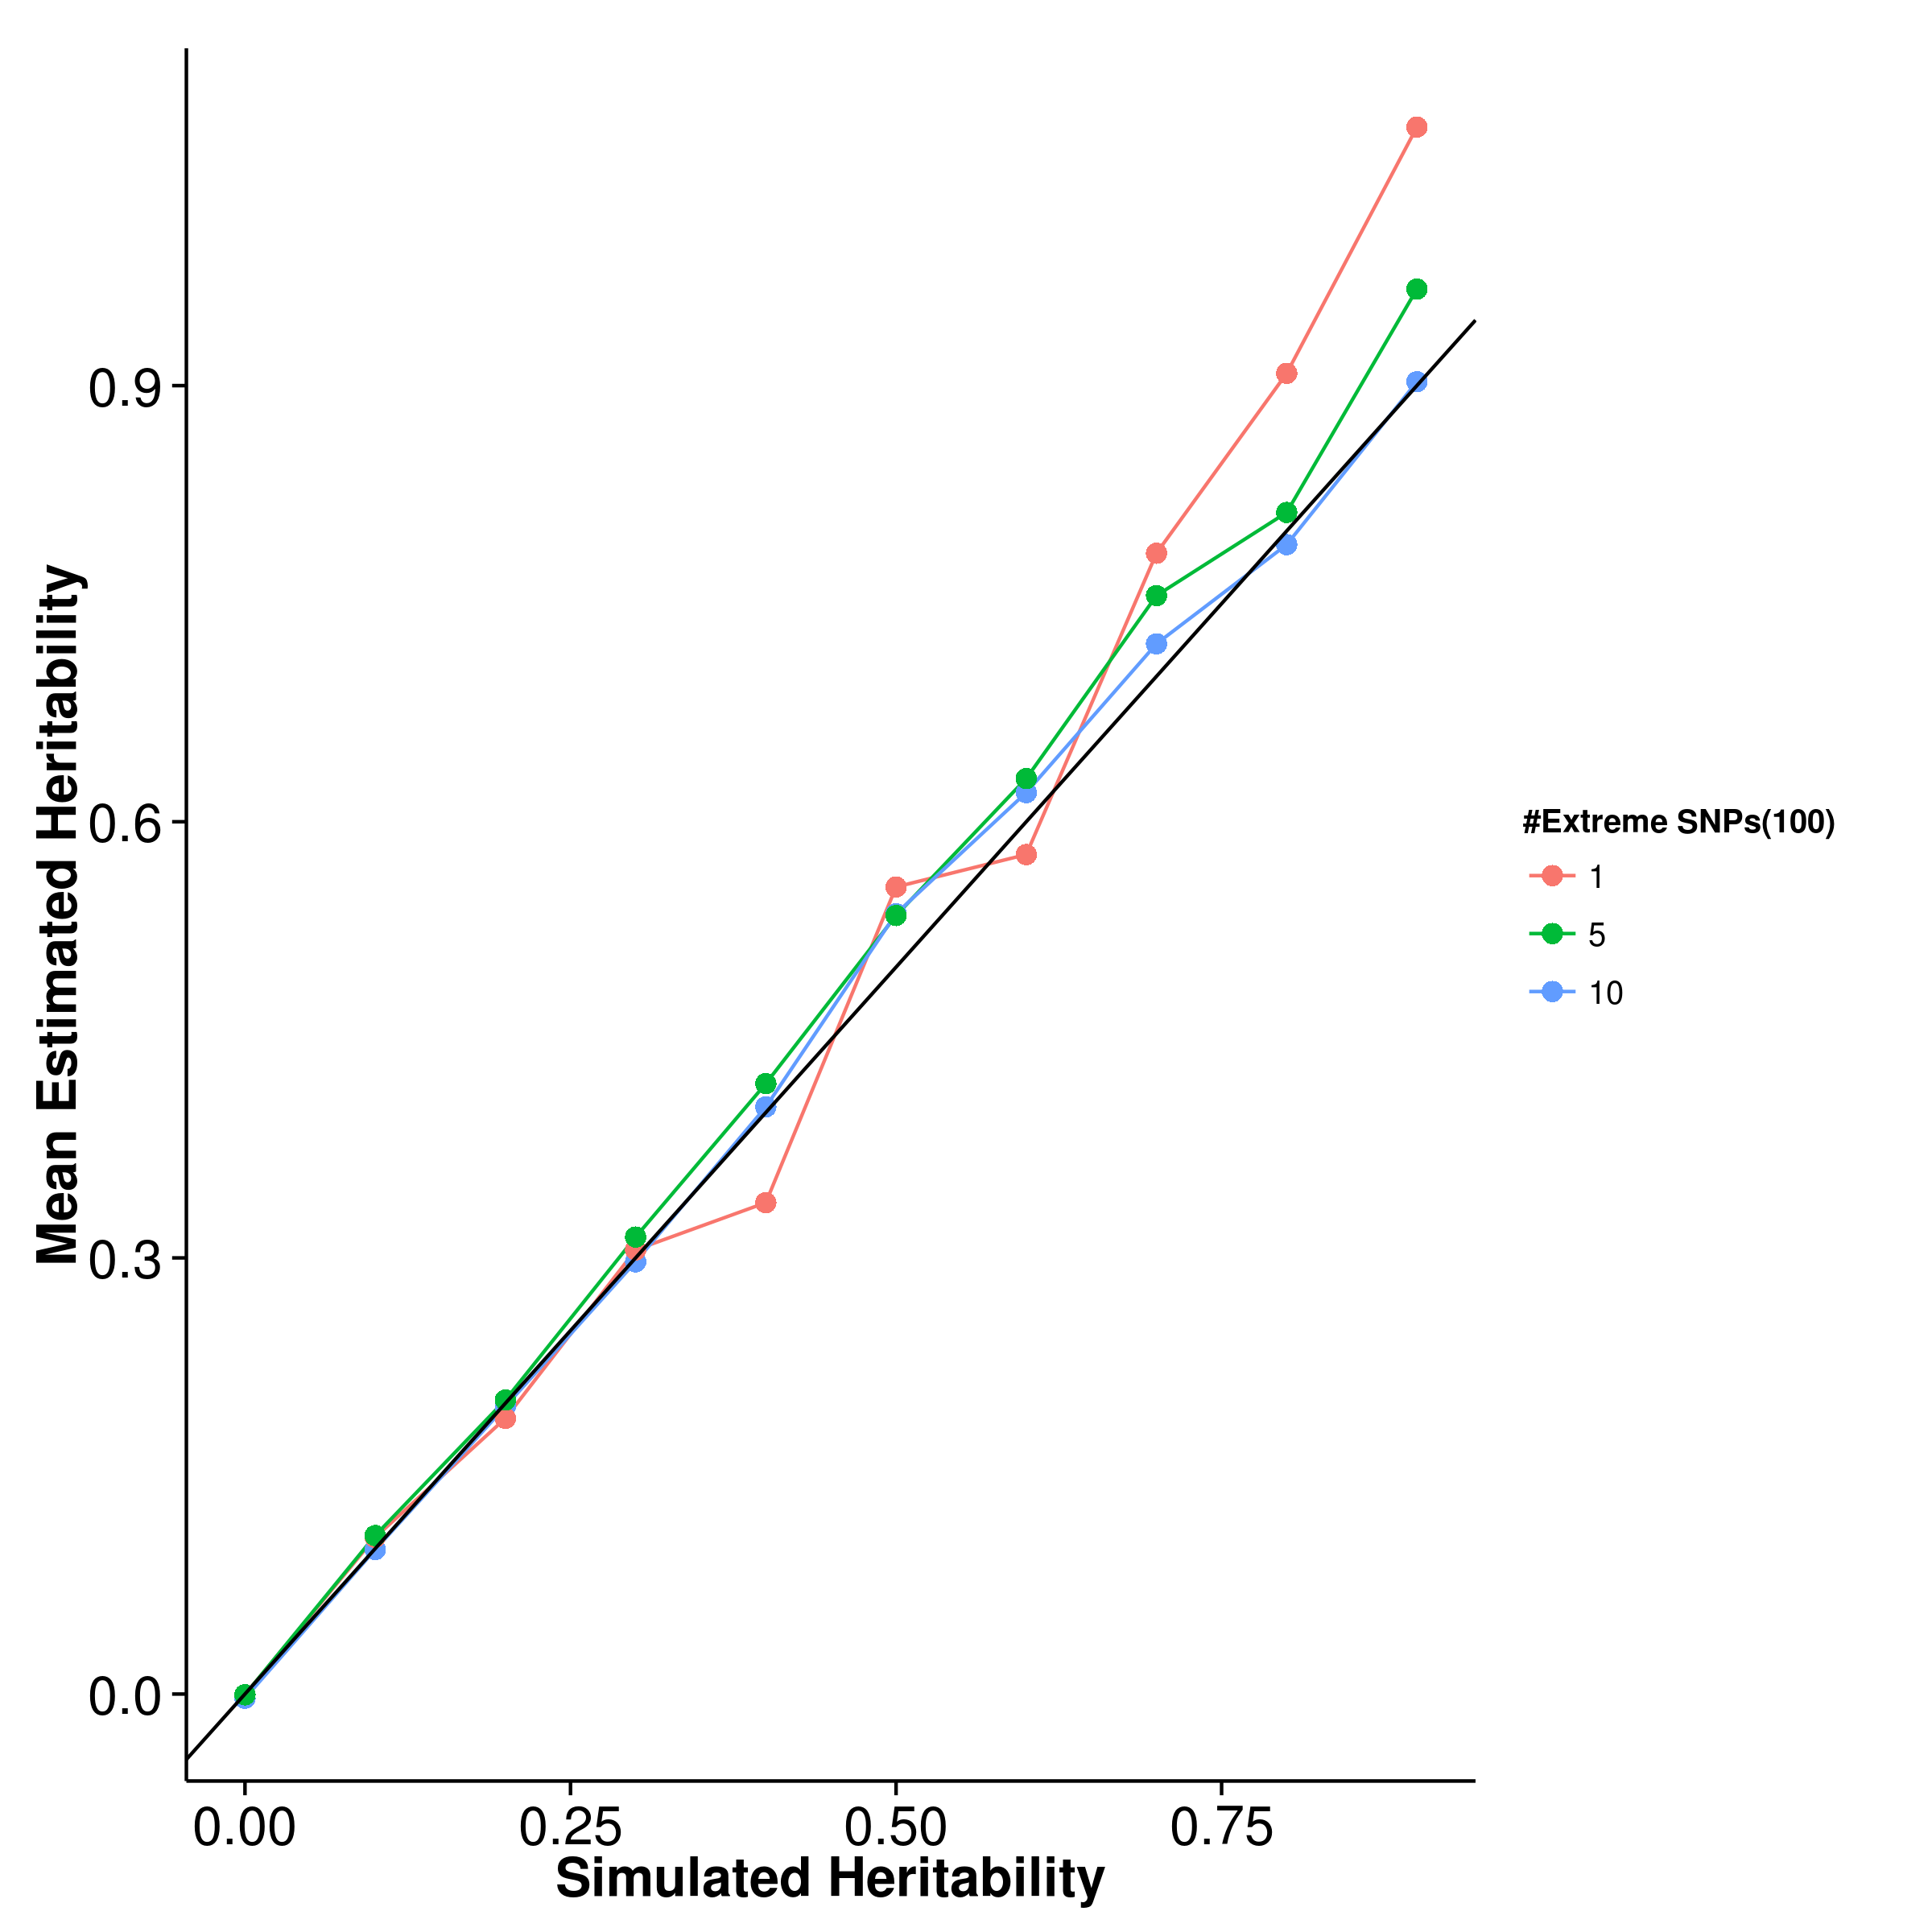
\includegraphics{figure/he_summary/extreme_100c/ldsc_QtE_Rand_mean.png}}
				\label{fig:ldscQtEx100cMean}
			}
			\subfloat[LDSC with intercept estimation]{
				
				\scalebox{.4}{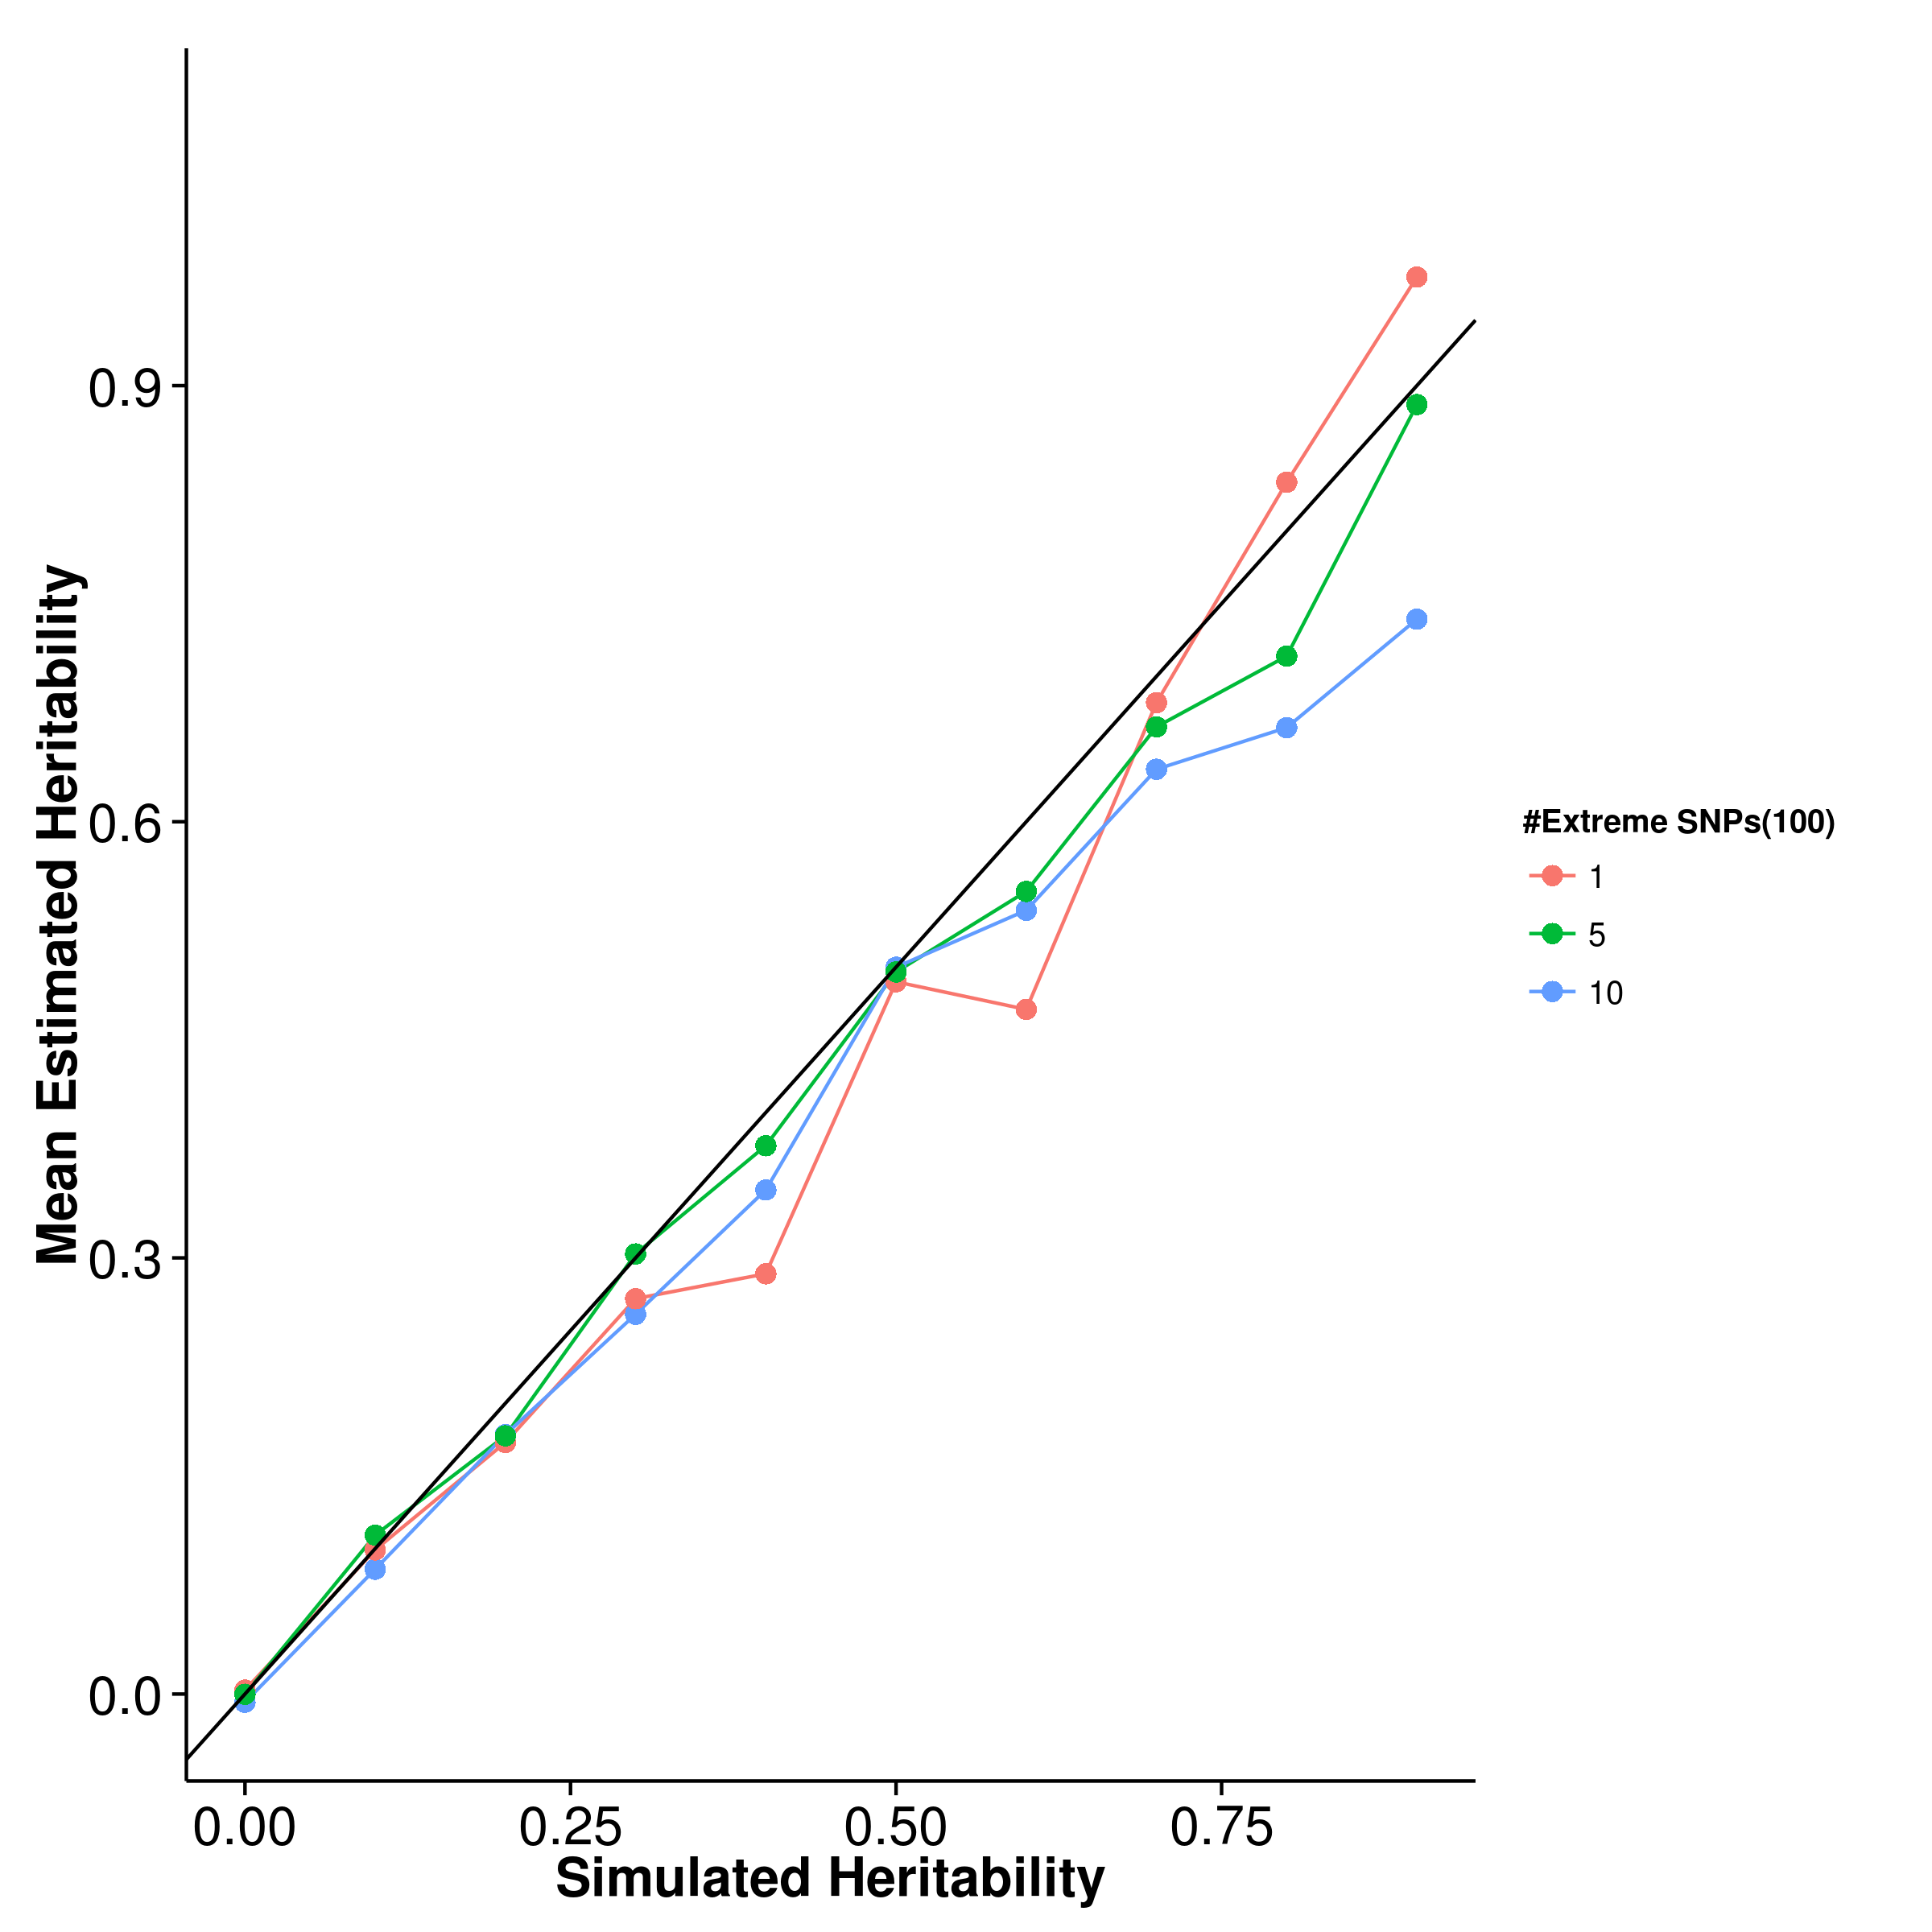
\includegraphics{figure/he_summary/extreme_100c/ldscIn_QtE_Rand_mean.png}}
				\label{fig:ldscInQtEx100cMean}
			}
			\caption[Mean of Extreme Effect Size Simulation Result]
			{Mean of results from quantitative trait simulation with extreme effect size simulation.
				It was observed that the mean estimation of heritability of \gls{shrek} is not affected by the number of \gls{SNP}(s) with large effect but with slight upward bias.
				On the other hand, the mean estimation of \gls{ldsc} and \gls{gcta} seems to fluctuate with respect to the simulated heritability.
				} 
			\label{fig:QtEx100cMean}
		\end{figure}
		
		\begin{figure}
			\centering
			\subfloat[SHREK]{
				\scalebox{.4}{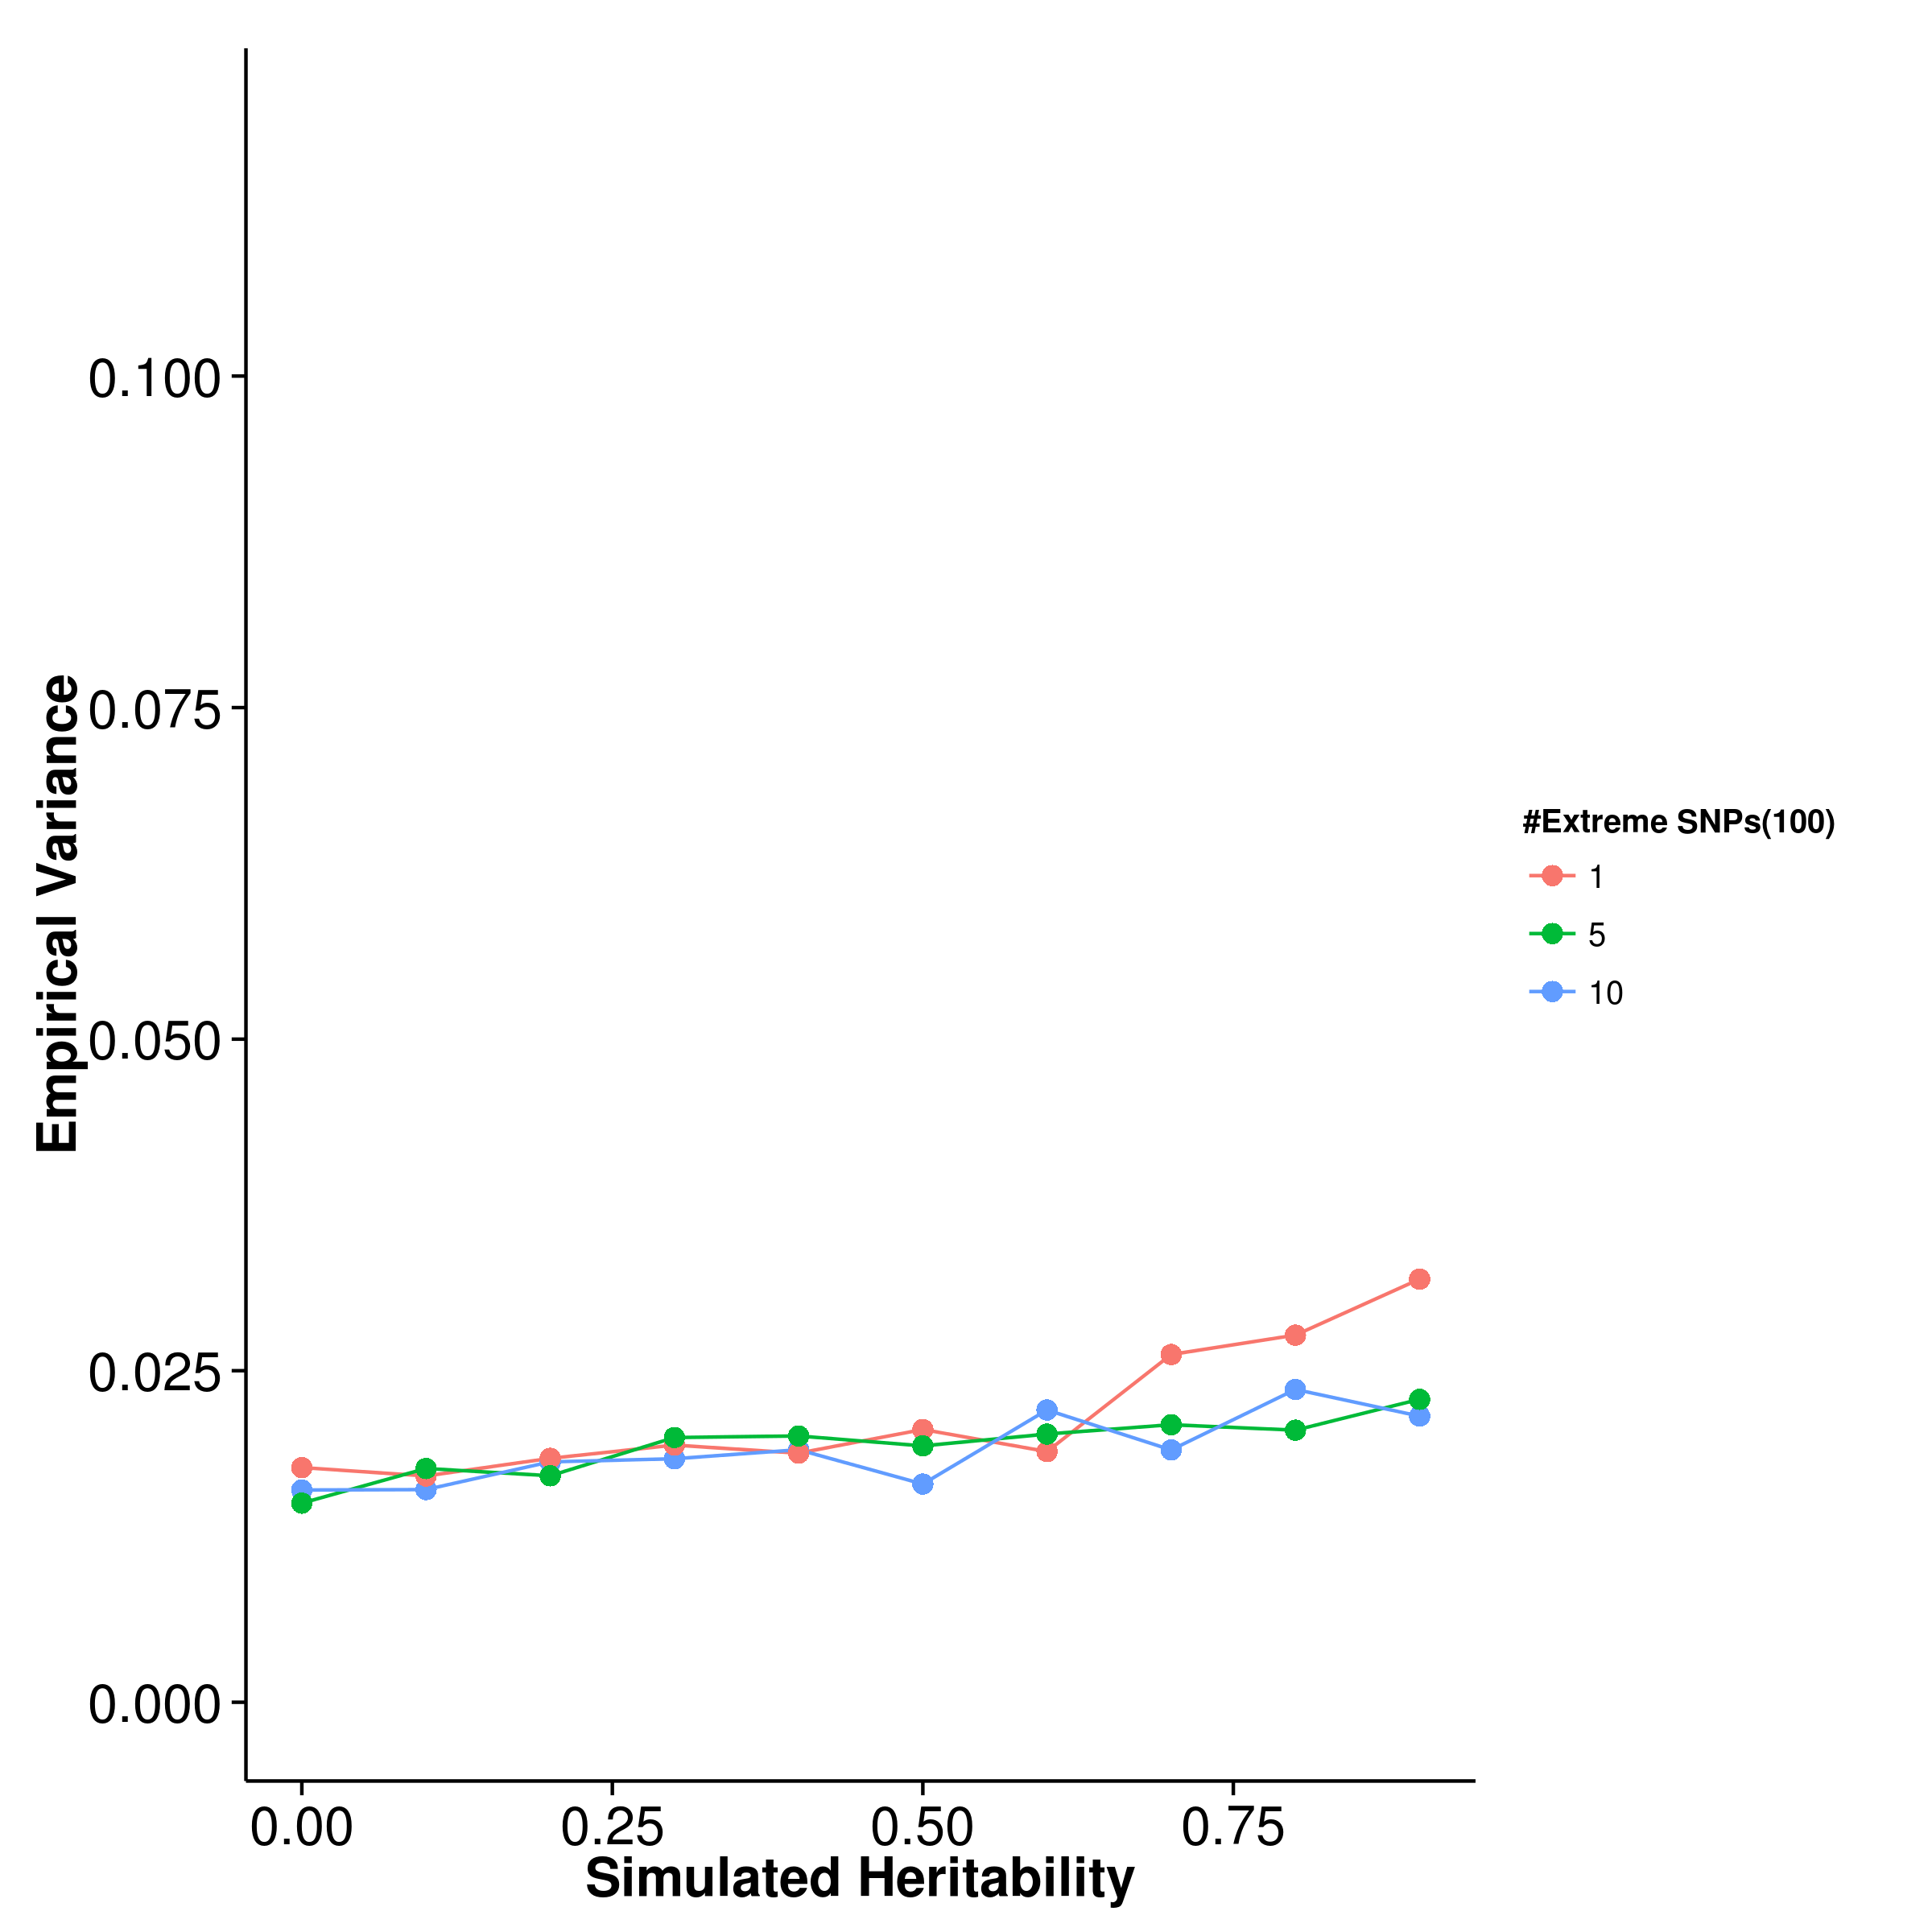
\includegraphics{figure/he_summary/extreme_100c/shrek_QtE_Rand_sd.png}}
				\label{fig:shrekQtEx100cVar}
			}
			\subfloat[GCTA]{
				\scalebox{.4}{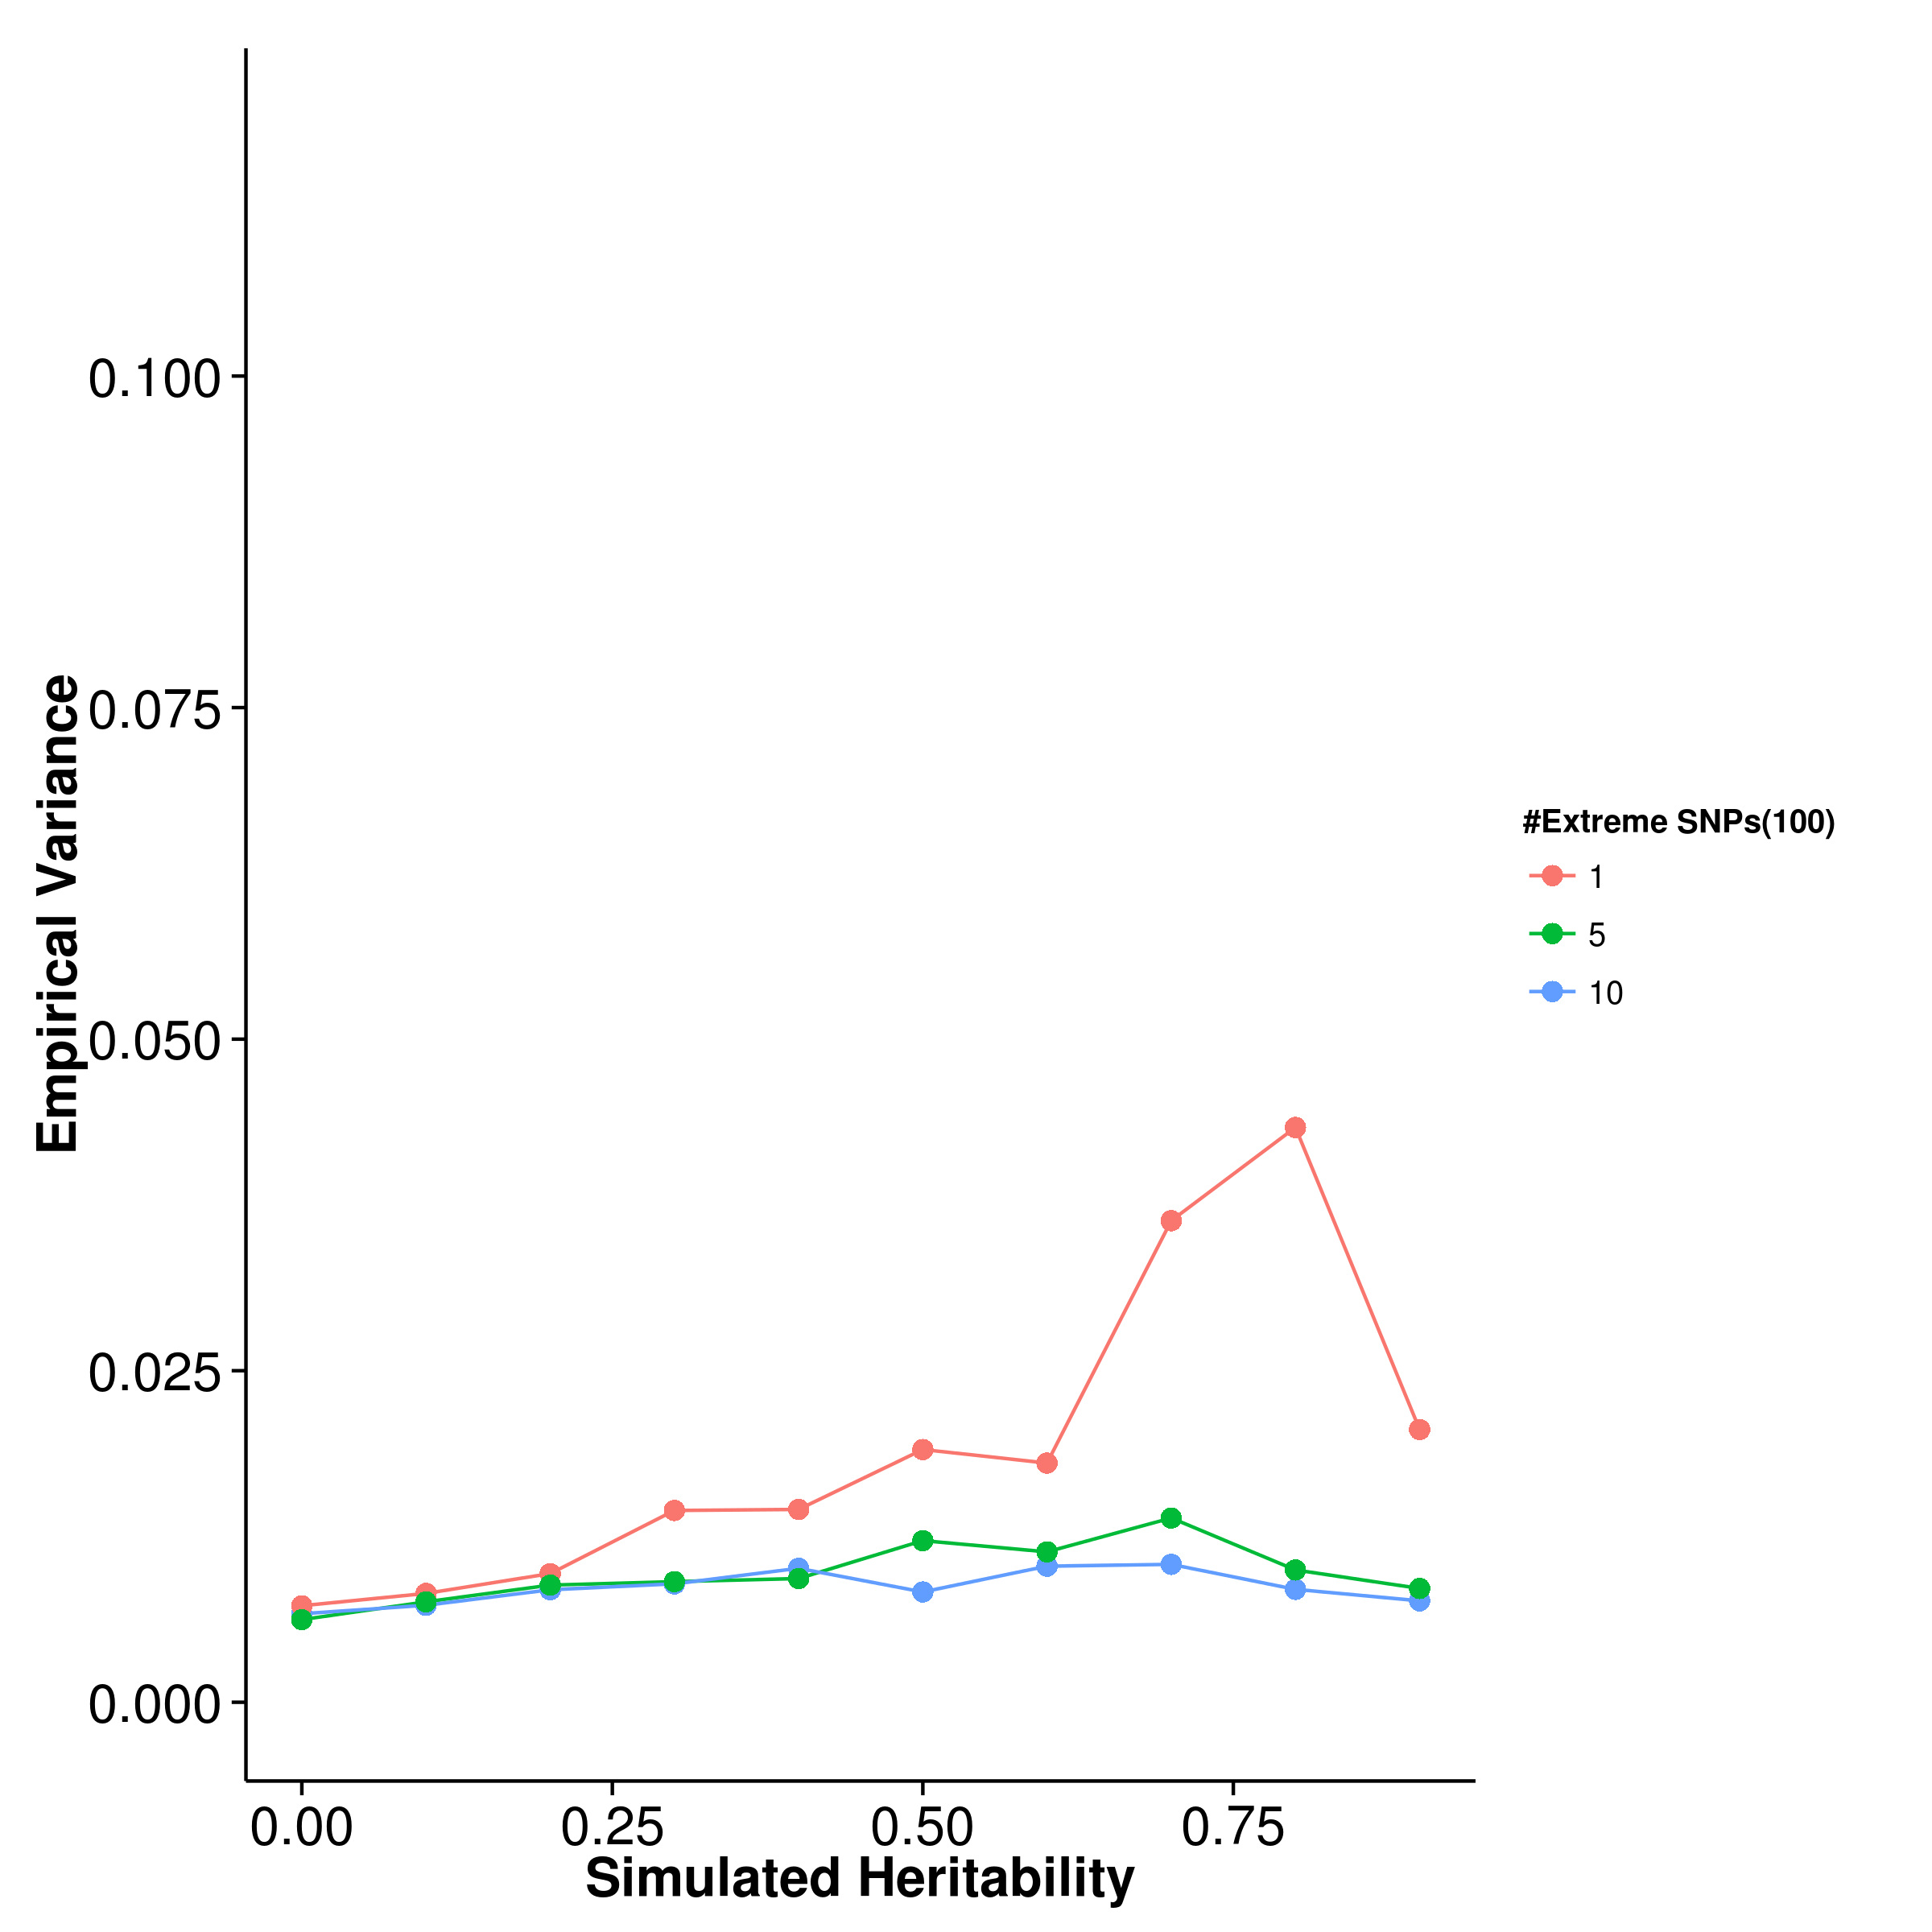
\includegraphics{figure/he_summary/extreme_100c/gcta_QtE_Rand_sd.png}}
				\label{fig:gctaQtEx100cVar}
			}\\
			\subfloat[LDSC with fix intercept]{
				\scalebox{.4}{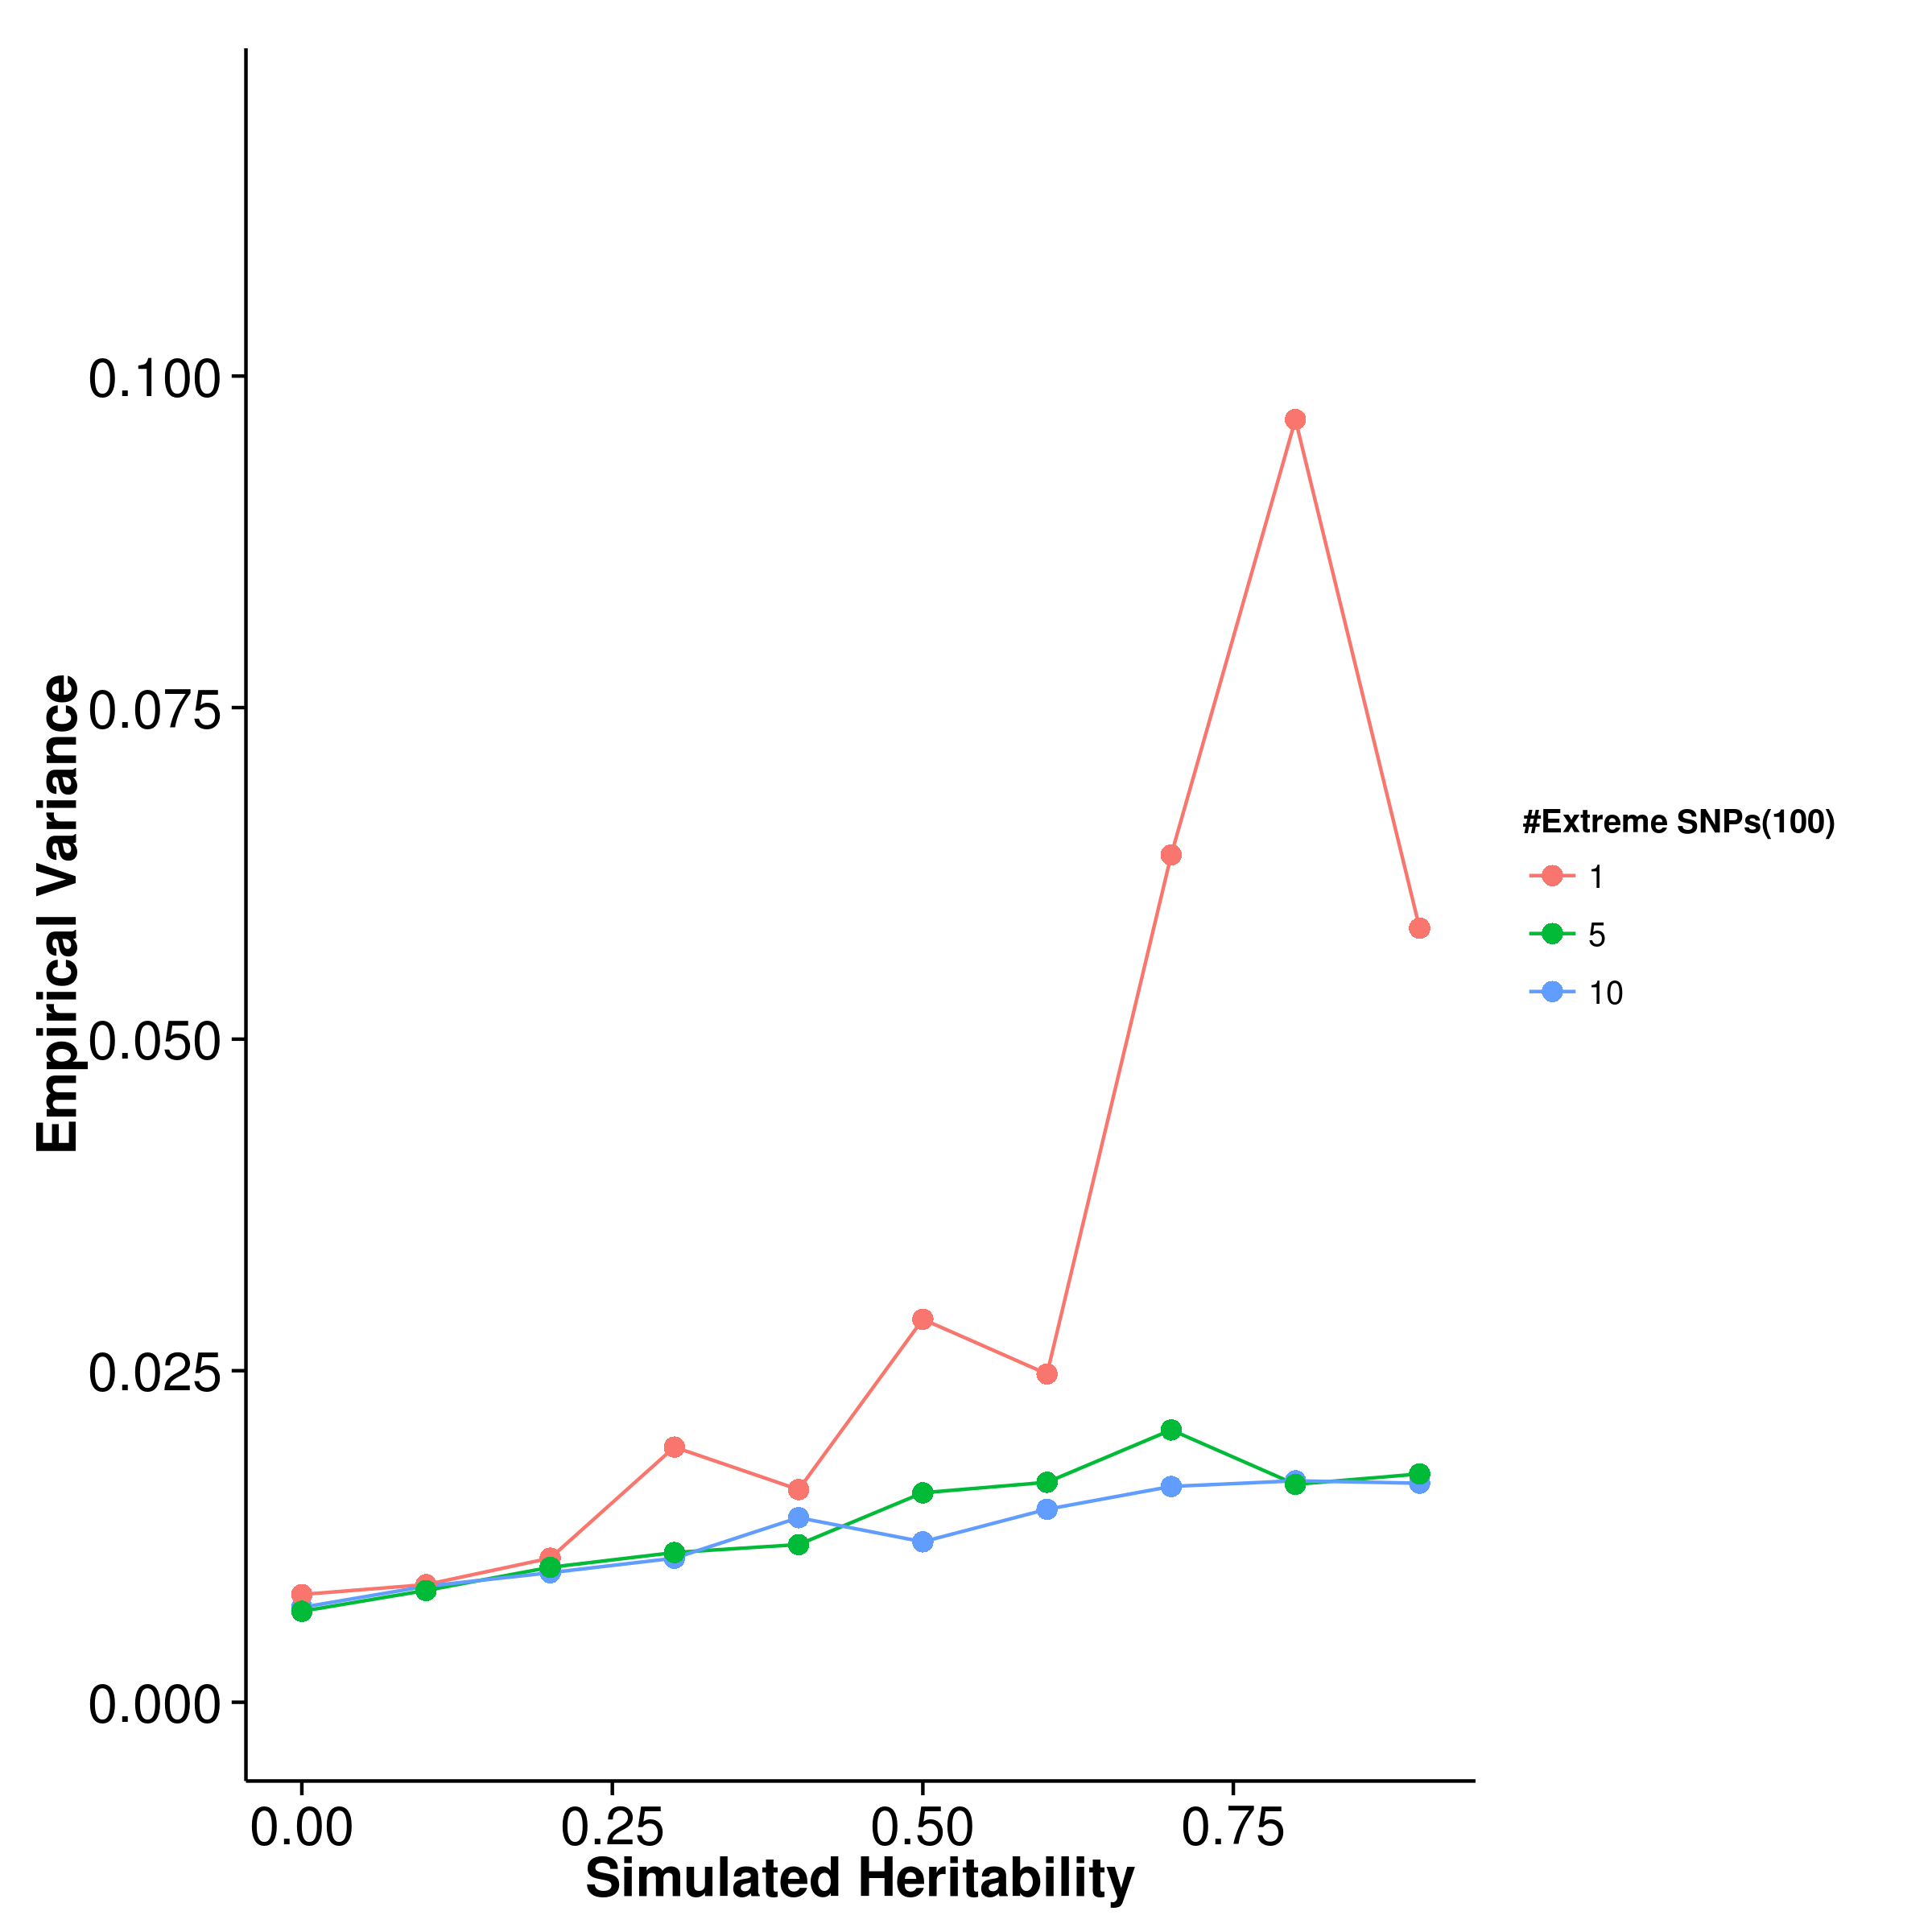
\includegraphics{figure/he_summary/extreme_100c/ldsc_QtE_Rand_sd.png}}
				\label{fig:ldscQtEx100cVar}
			}
			\subfloat[LDSC with intercept estimation]{
				
				\scalebox{.4}{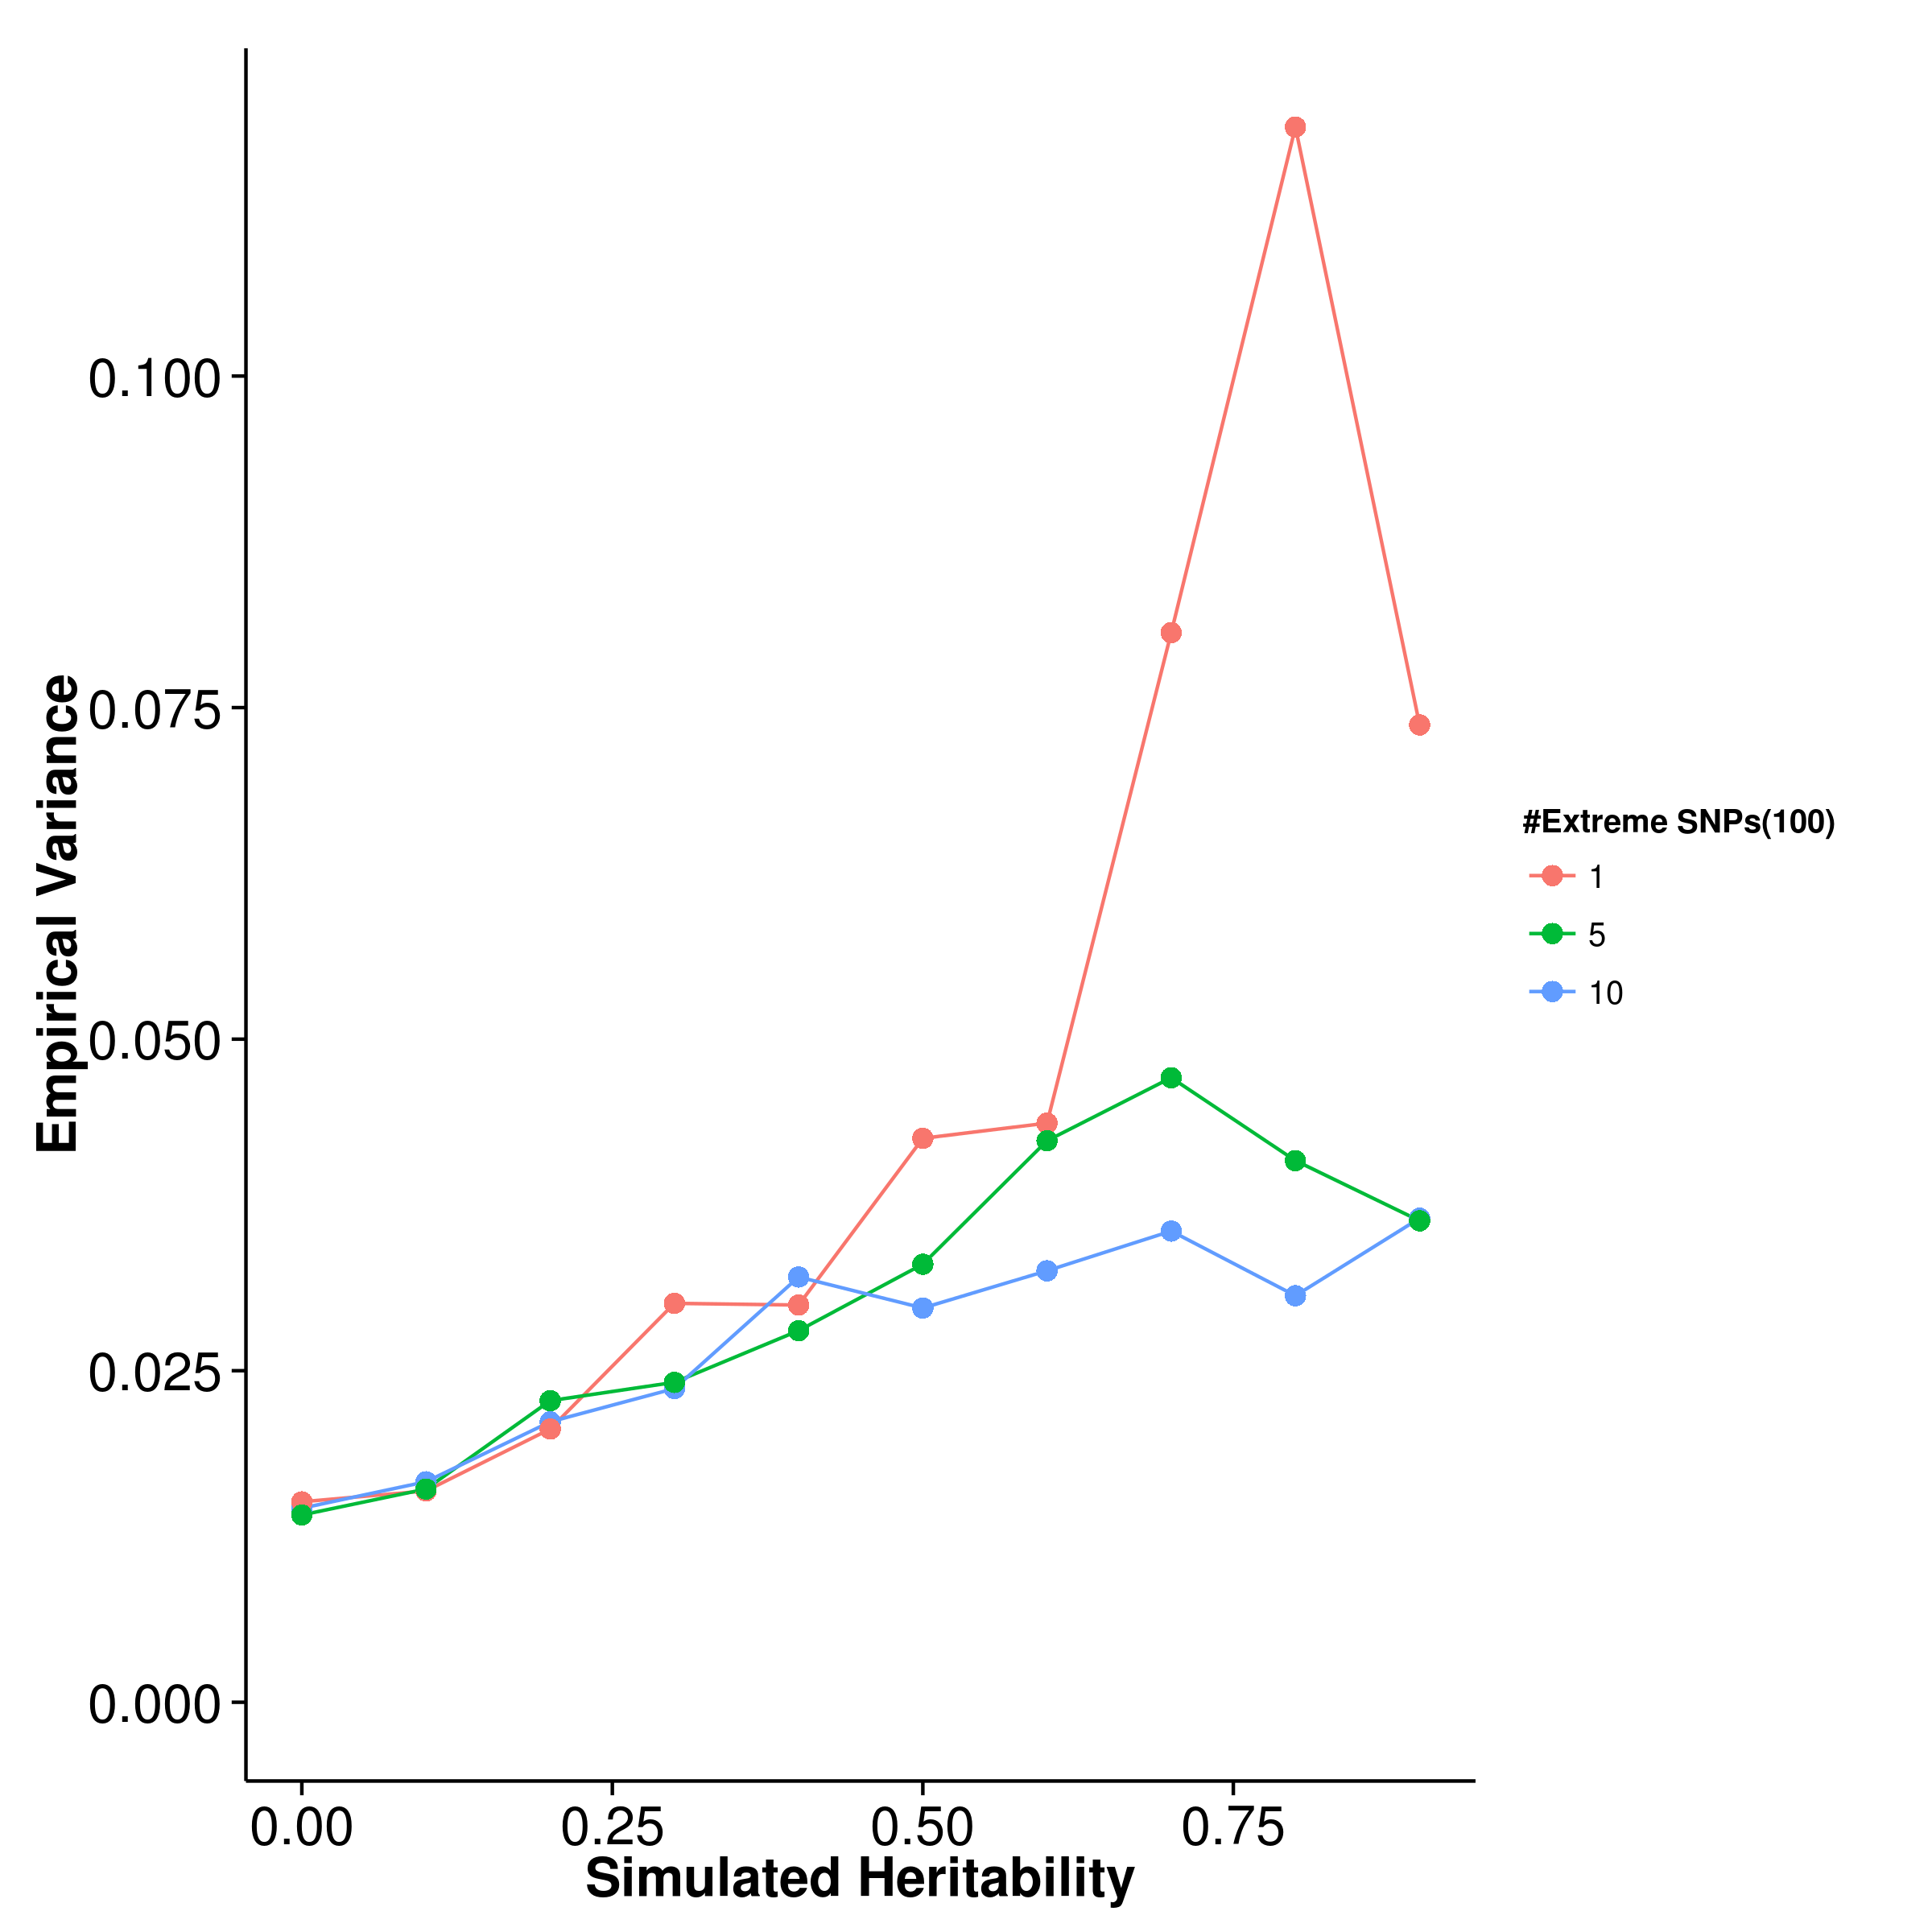
\includegraphics{figure/he_summary/extreme_100c/ldscIn_QtE_Rand_sd.png}}
				\label{fig:ldscInQtEx100cVar}
			}
			\caption[Variance of Extreme Effect Size Simulation Result]
			{Variance of results from quantitative trait simulation with extreme effect size simulation.
				100 causal \glspl{SNP} were simulated.
				When only 1 \gls{SNP} with extreme effect was simulated, the empirical variance of \gls{gcta} and \gls{ldsc} increases and a large fluctuation was observed.
				Whereas the empirical variance of \gls{shrek} only increase slightly when the simulated heritability is large and with only 1 \gls{SNP} with extreme effect.
				Suggesting that it is more robust to the change in number of extreme \gls{SNP}(s).
			} 
			\label{fig:QtEx100cVar}
		\end{figure}
		
		\begin{figure}
			\centering
			\subfloat[SHREK]{
				\scalebox{.4}{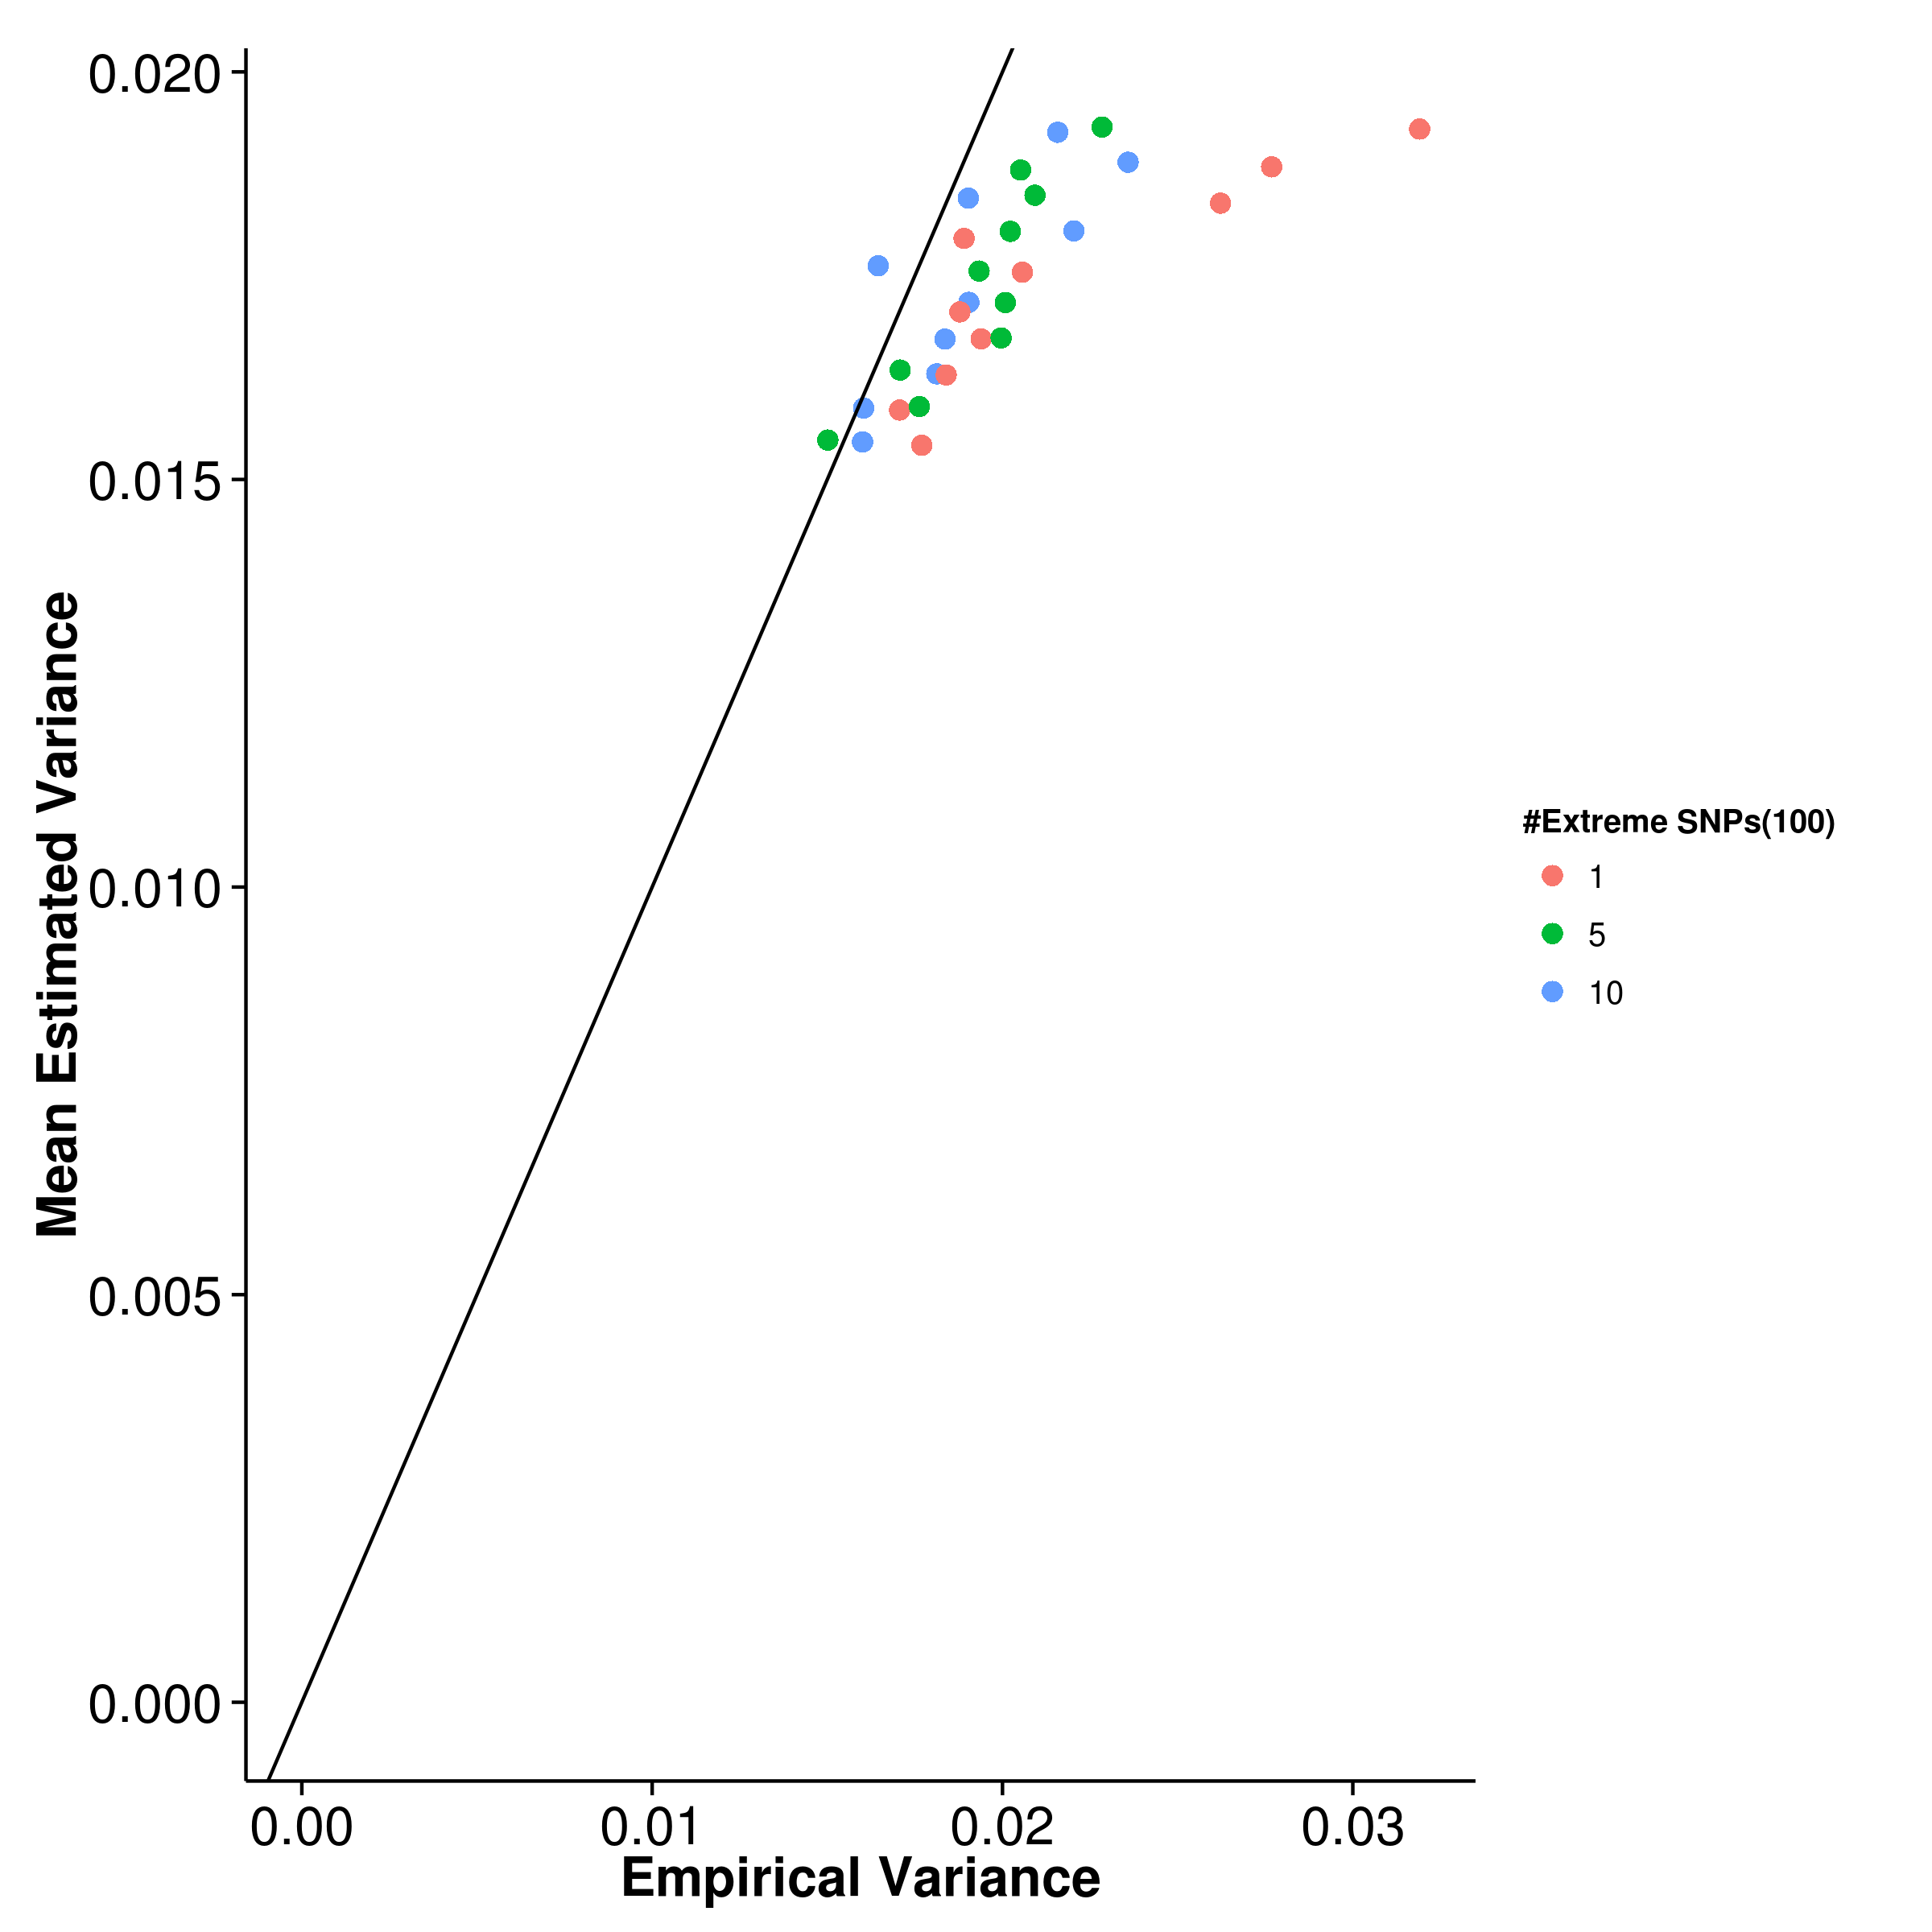
\includegraphics{figure/he_summary/extreme_100c/shrek_QtE_Rand_sdCom.png}}
				\label{fig:shrekQtEx100cVarCom}
			}
			\subfloat[GCTA]{
				\scalebox{.4}{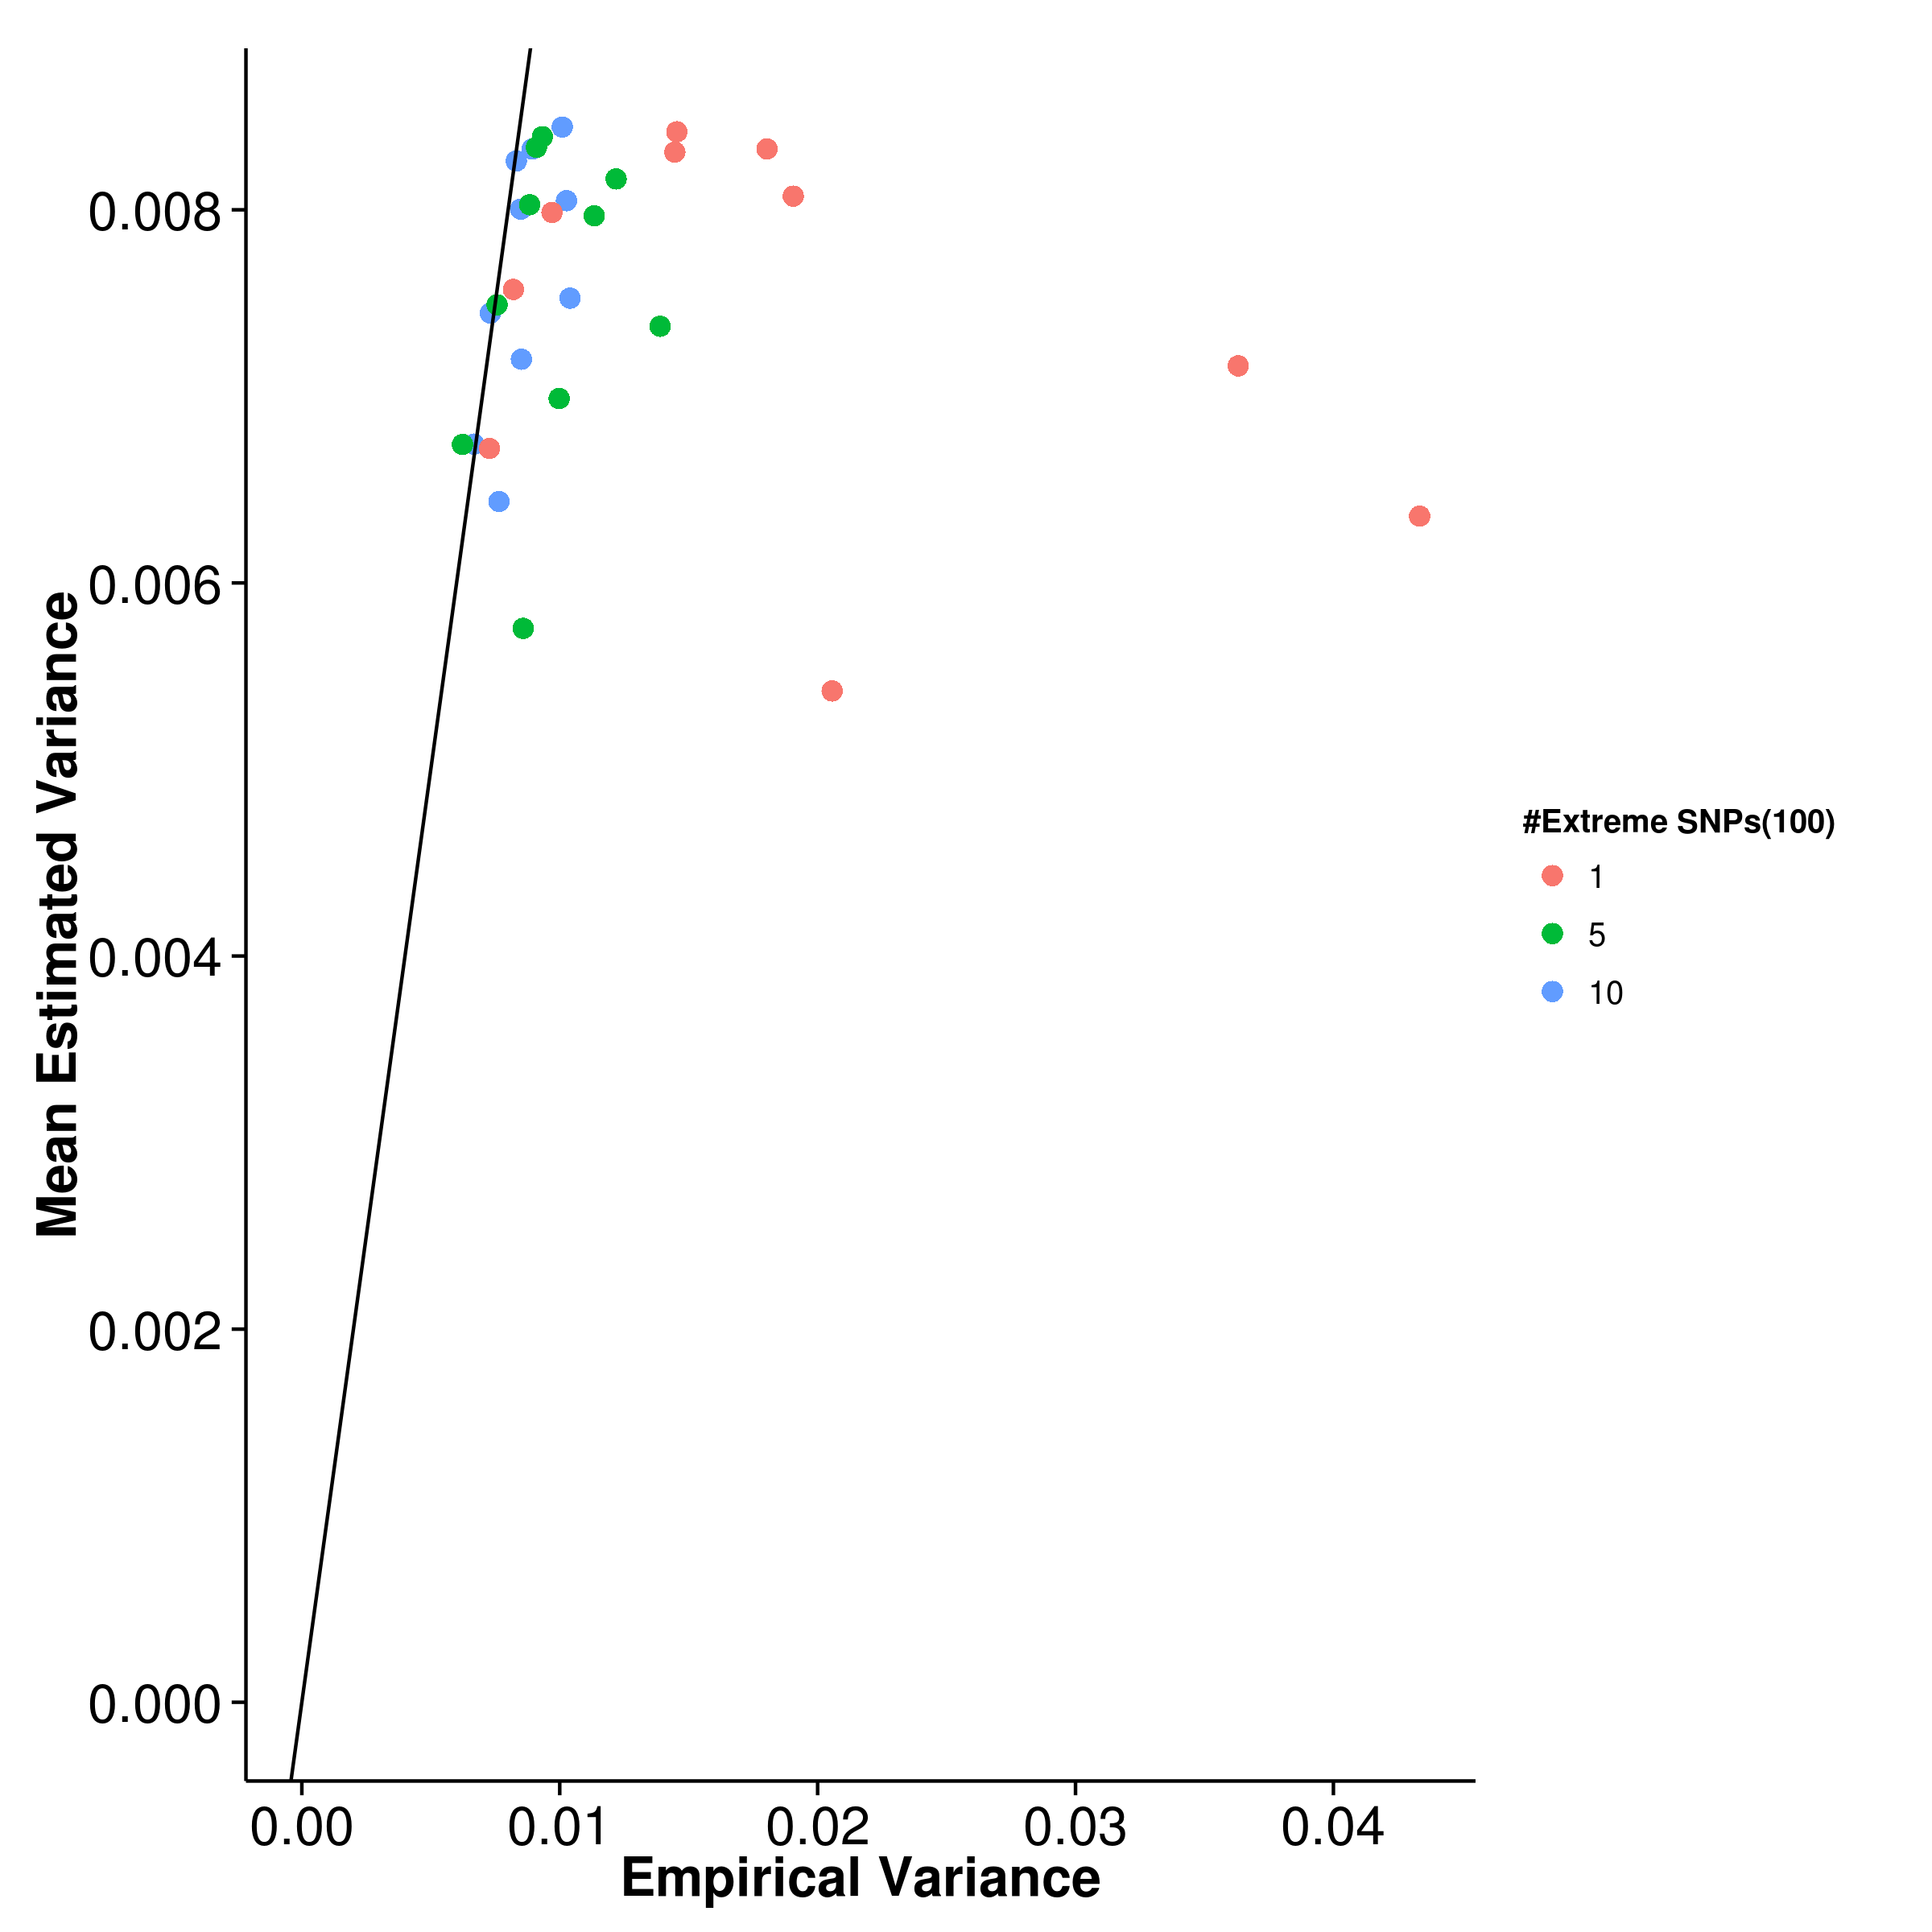
\includegraphics{figure/he_summary/extreme_100c/gcta_QtE_Rand_sdCom.png}}
				\label{fig:gctaQtEx100cVarCom}
			}\\
			\subfloat[LDSC with fix intercept]{
				\scalebox{.4}{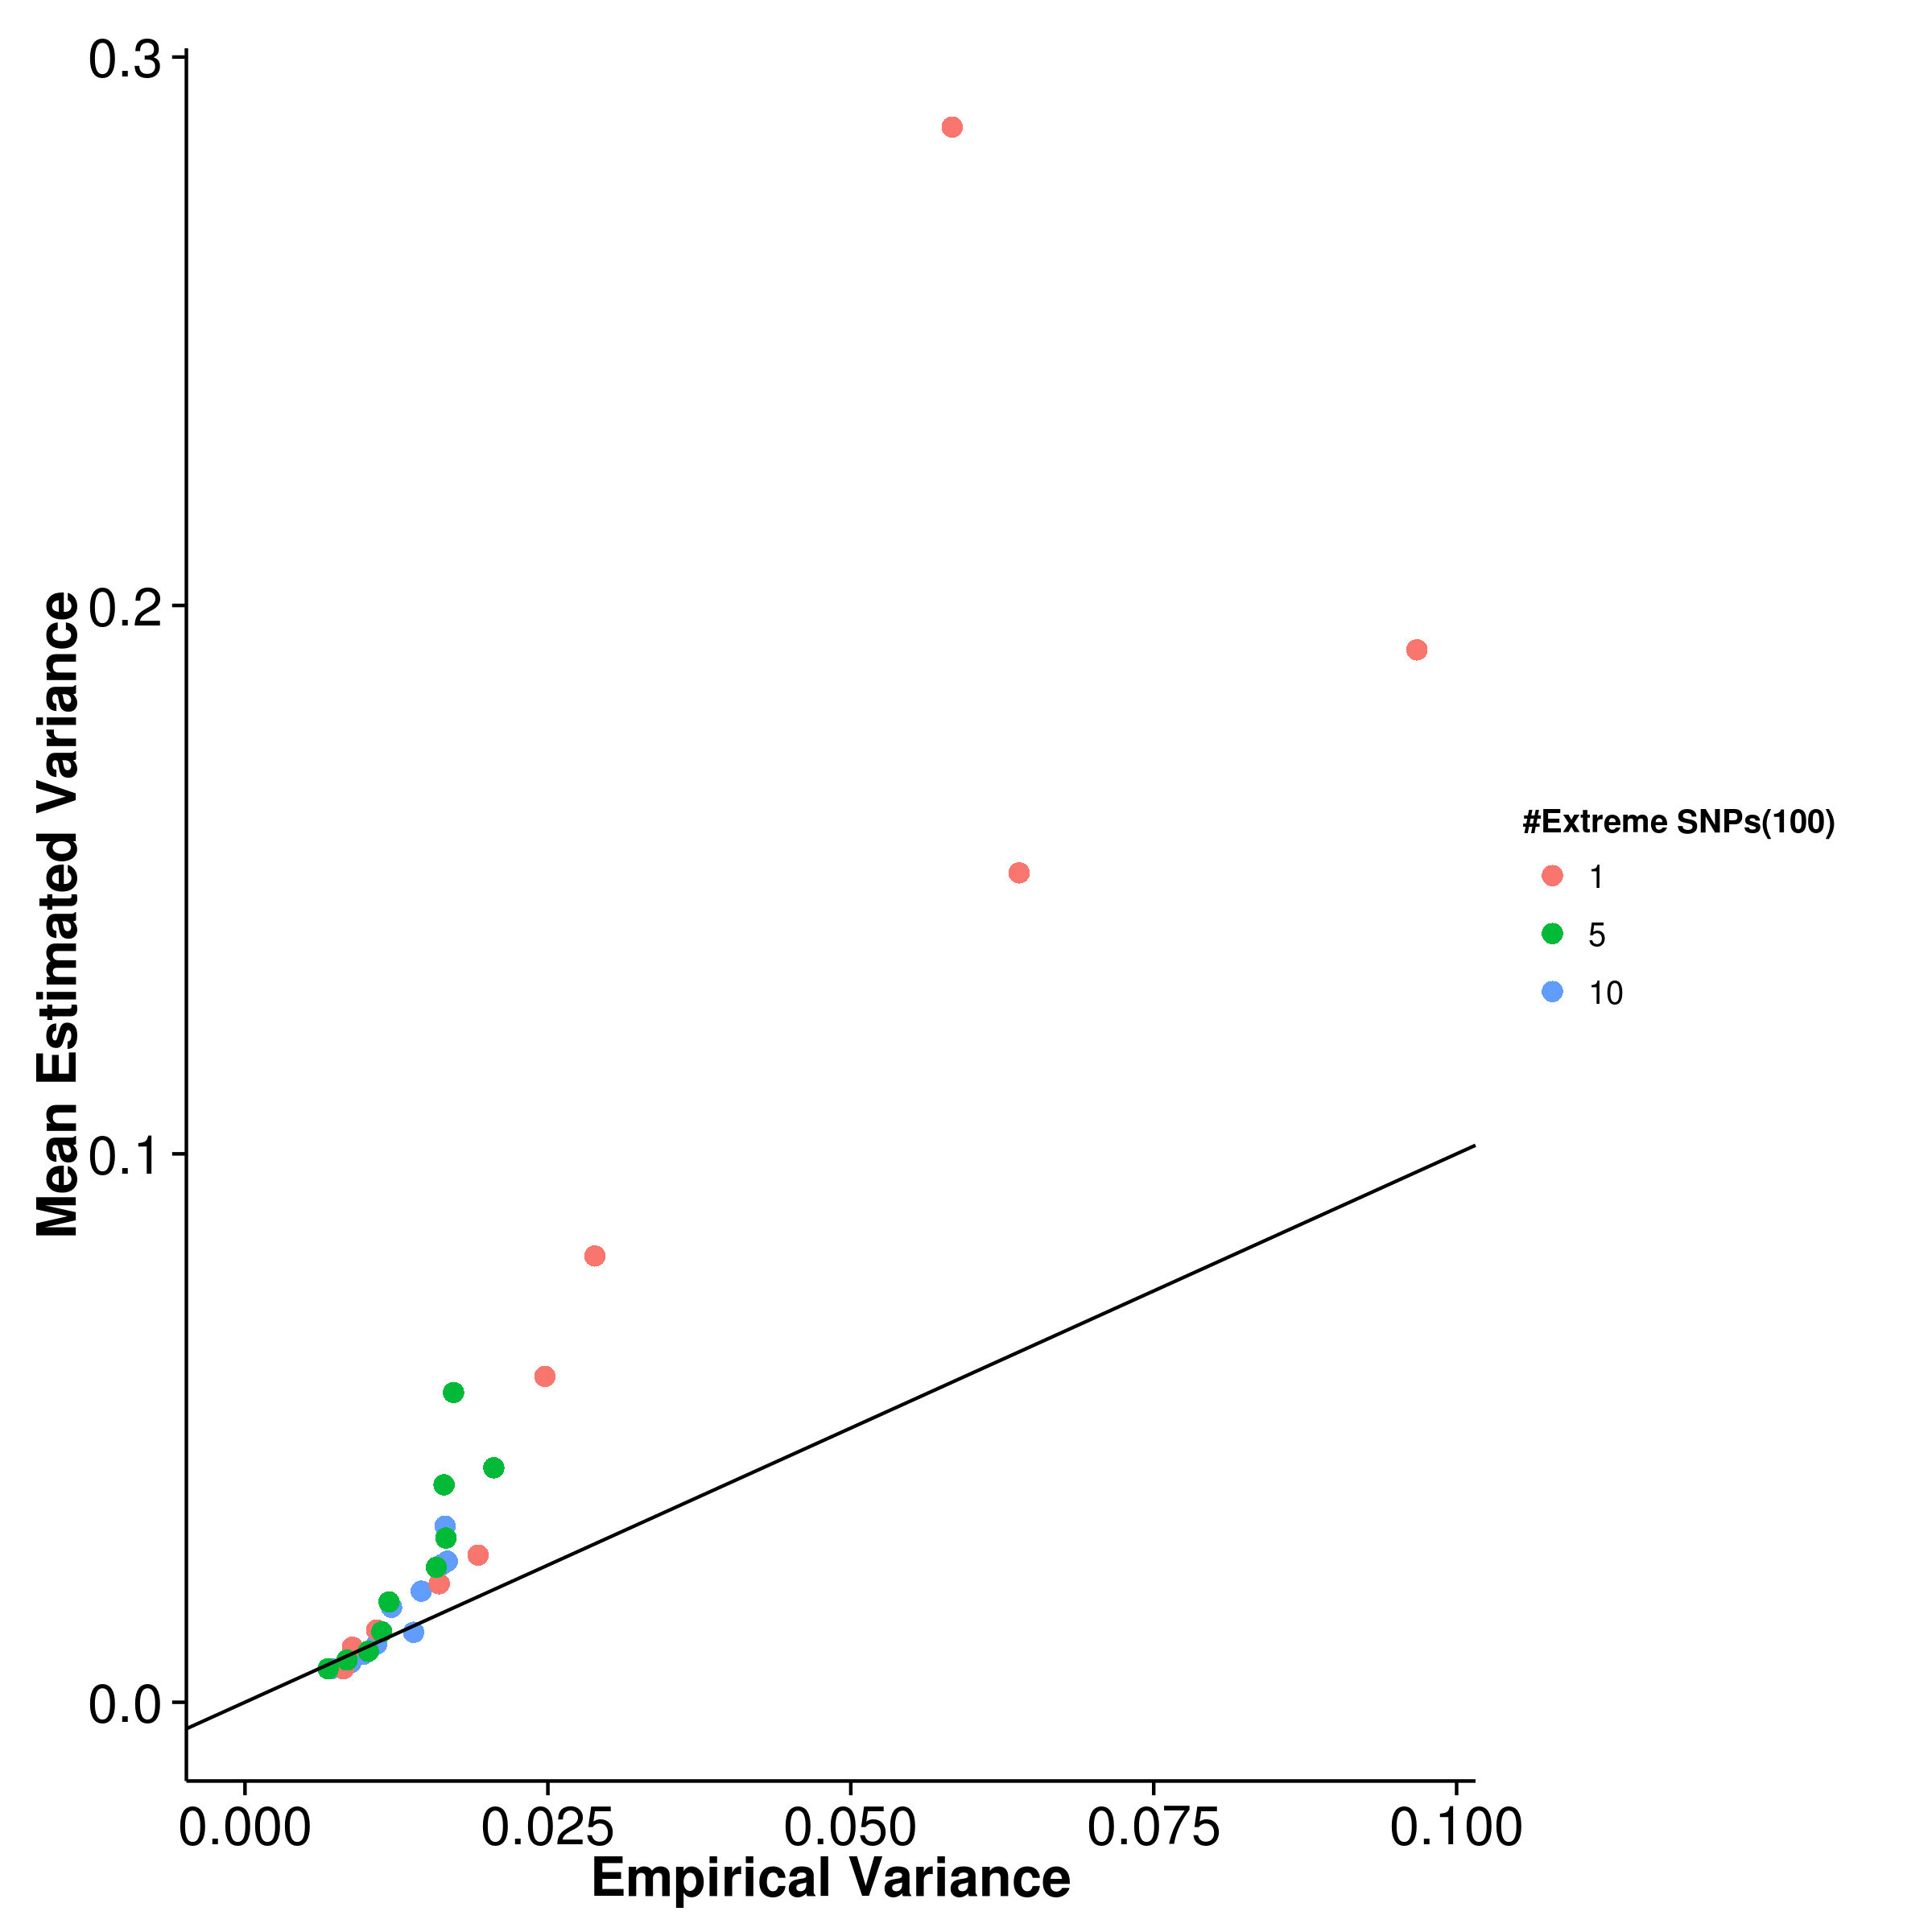
\includegraphics{figure/he_summary/extreme_100c/ldsc_QtE_Rand_sdCom.png}}
				\label{fig:ldscQtEx100cVarCom}
			}
			\subfloat[LDSC with intercept estimation]{
				
				\scalebox{.4}{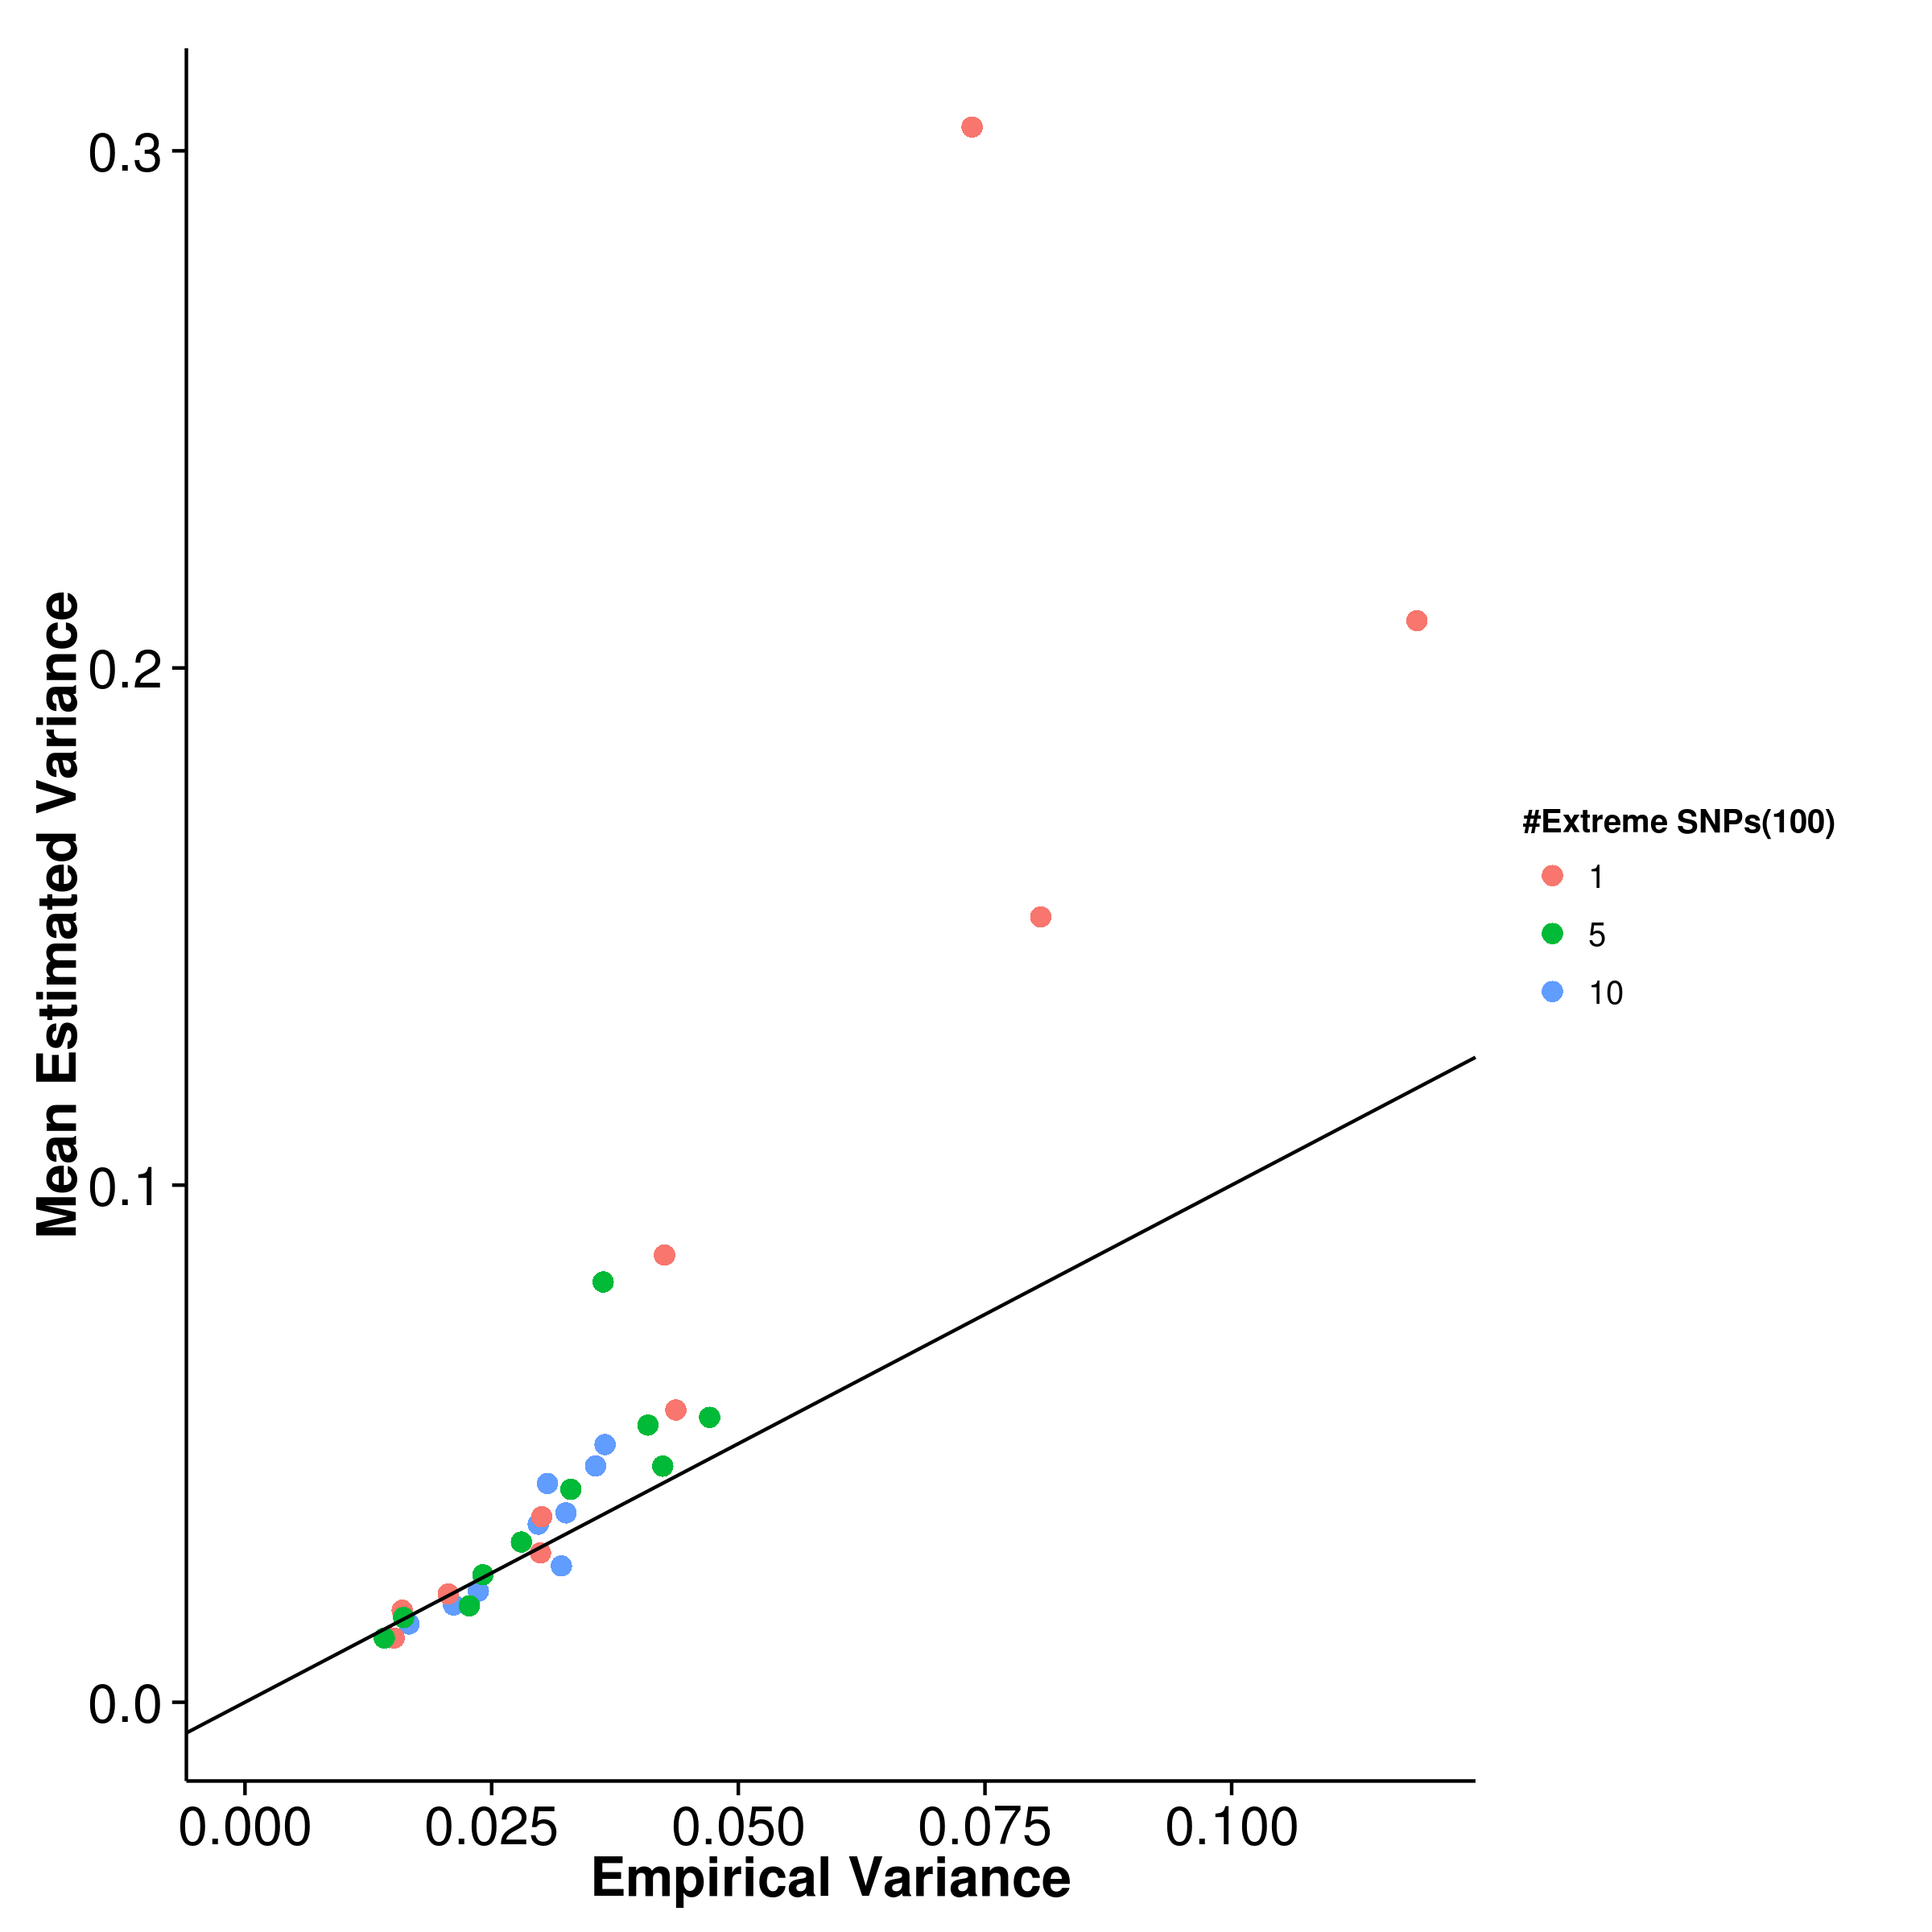
\includegraphics{figure/he_summary/extreme_100c/ldscIn_QtE_Rand_sdCom.png}}
				\label{fig:ldscInQtEx100cVarCom}
			}
			\caption[Estimation of Variance in Extreme Effect Size Simulation]
			{Estimated variance of results from quantitative trait simulation with extreme effect size simulation when compared to the empirical variance.
				100 causal \glspl{SNP} were simulated.
				\gls{shrek} and \gls{gcta} generally under-estimate the variance with the magnitude of bias being the highest when there is only 1 \gls{SNP} with extreme effect.
				On the other hand, \gls{ldsc} tends to over-estimate the variance and it can overestimate the variance by more than 3 folds when there is only 1 \gls{SNP} with extreme effect.
			} 
			\label{fig:QtEx100cVarCom}
		\end{figure}
		Another condition that we were interested in was in the case where a small portion of \glspl{SNP} has a much larger effect than other \glspl{SNP}.
		In this simulation, we simulated either 100 or 250 causal \glspl{SNP} with 1, 5 or 10 \glspl{SNP} having a much larger effect.
		
		% Extreme with 250 causal
		
		\begin{figure}
			\centering
			\subfloat[SHREK]{
				\scalebox{.4}{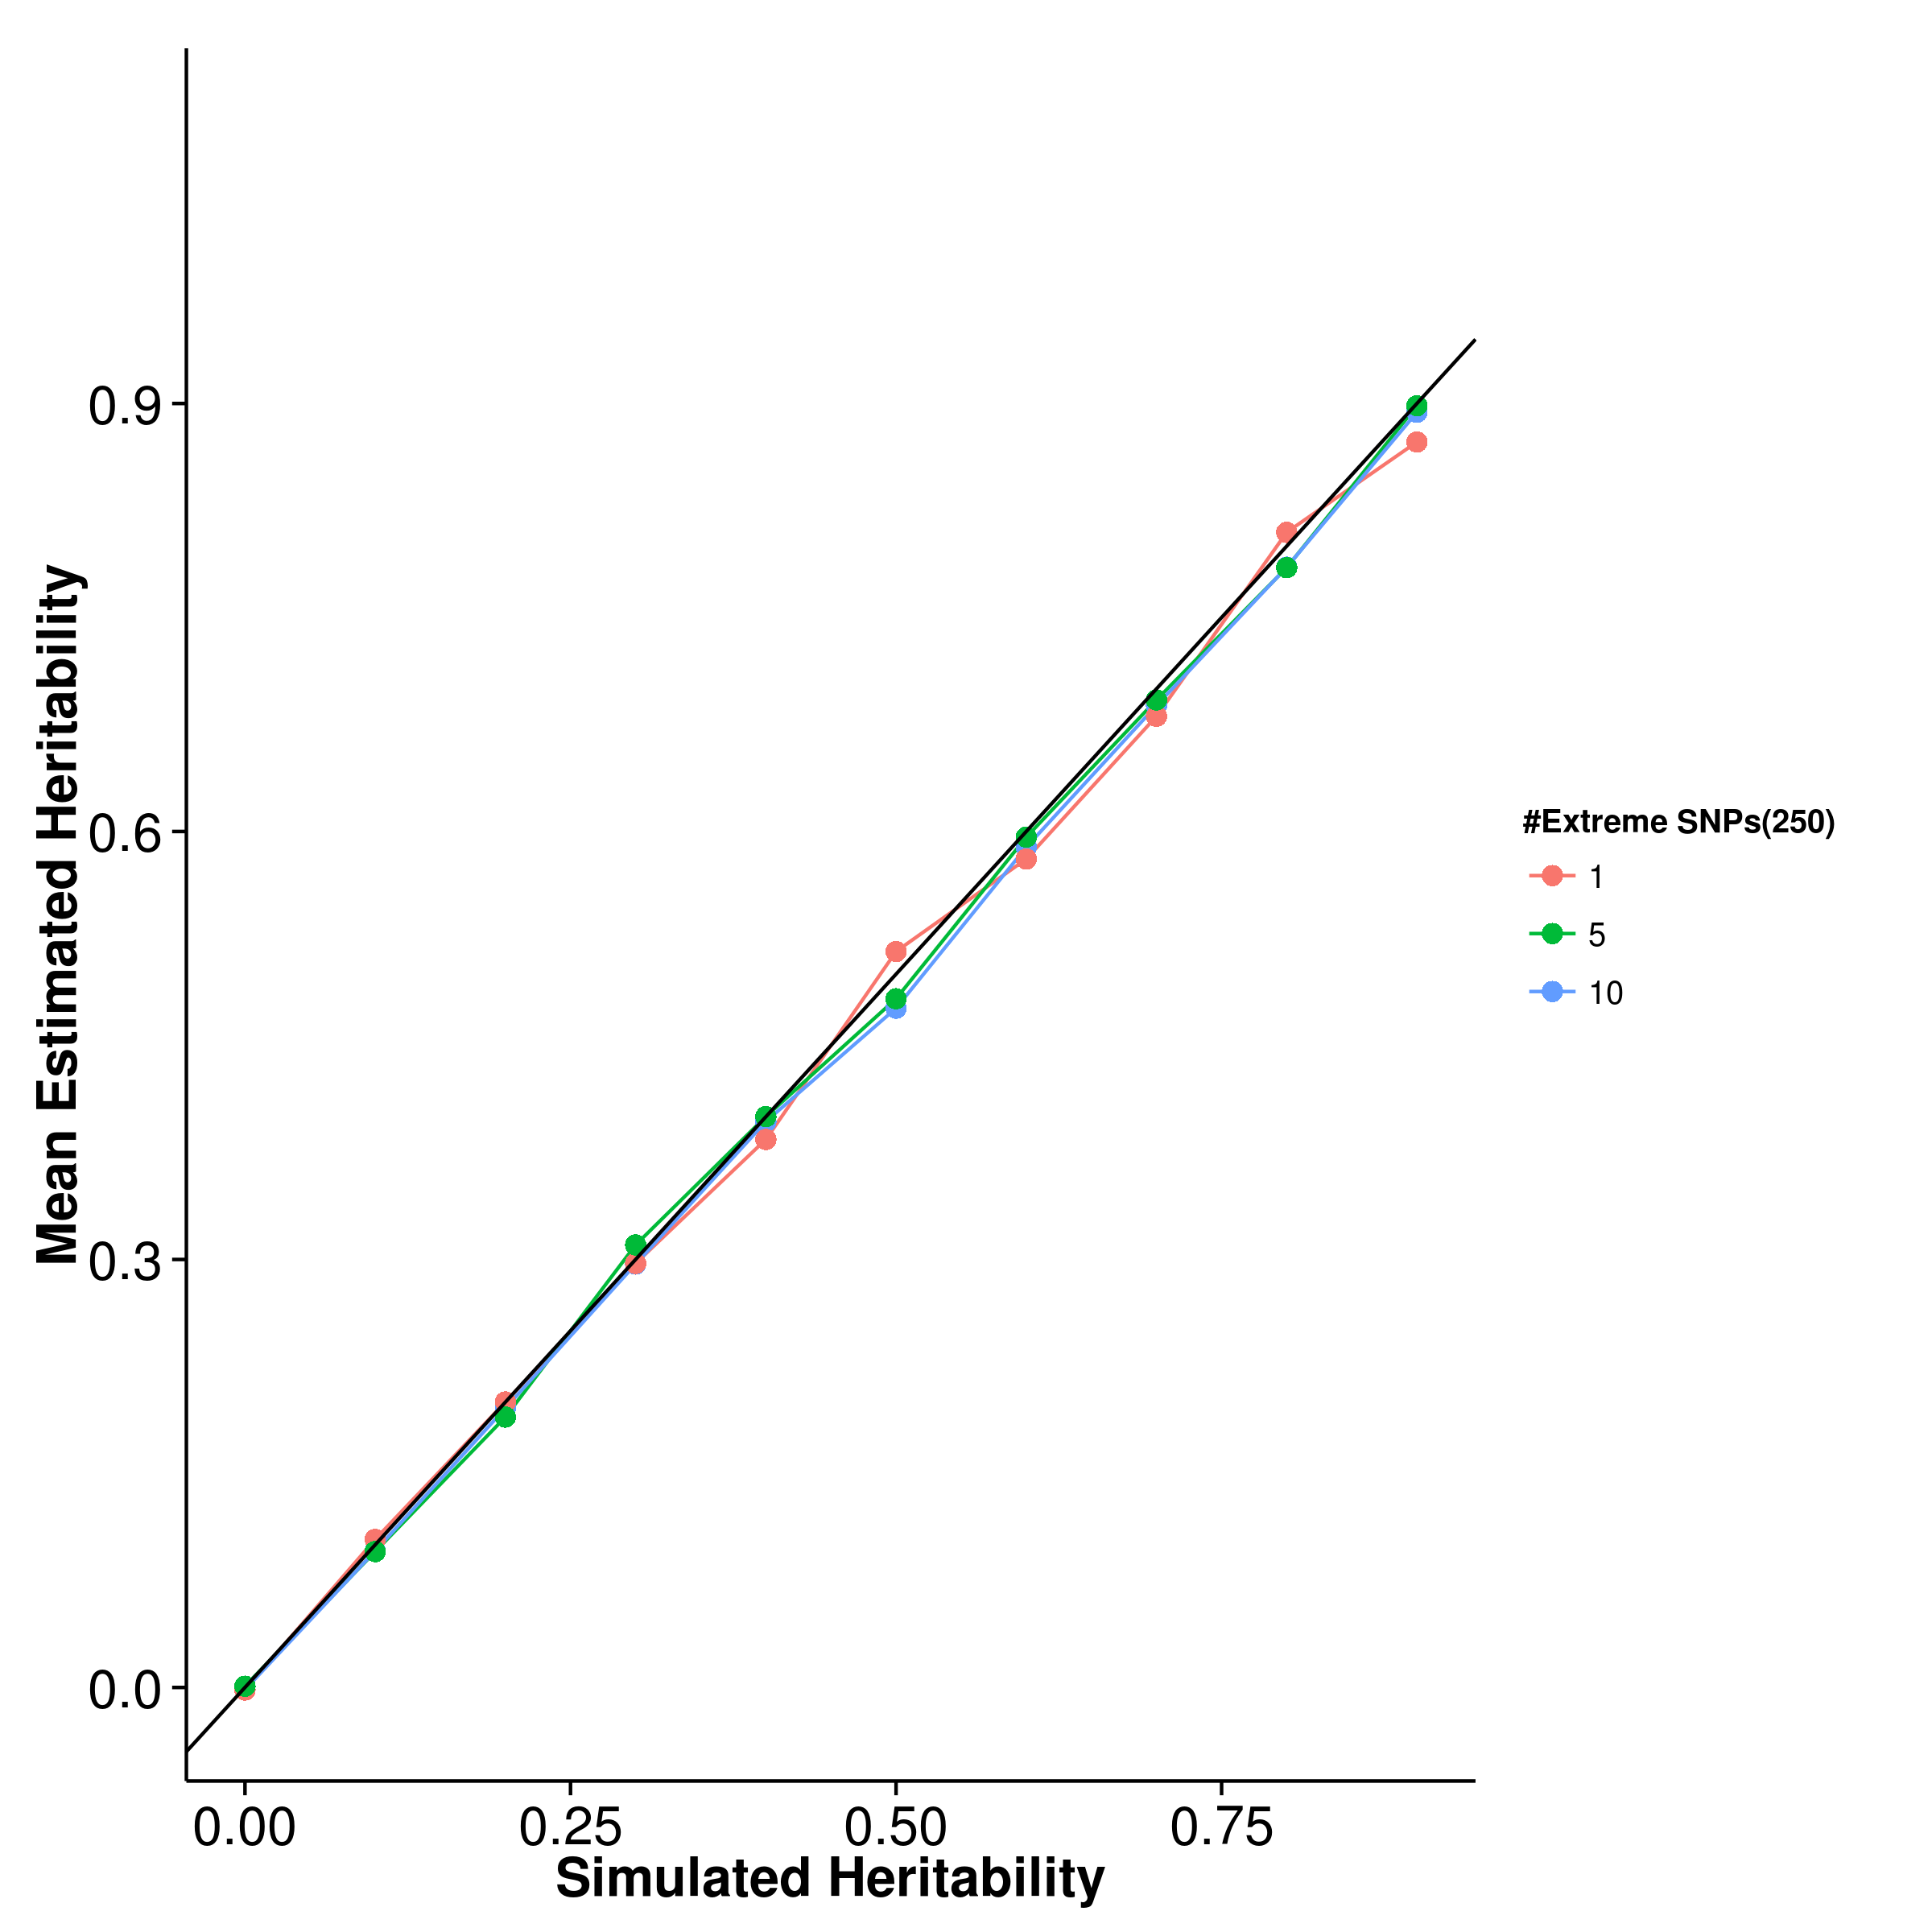
\includegraphics{figure/he_summary/extreme_250c/shrek_QtE_Extreme_mean.png}}
				\label{fig:shrekQtEx250cMean}
			}
			\subfloat[GCTA]{
				\scalebox{.4}{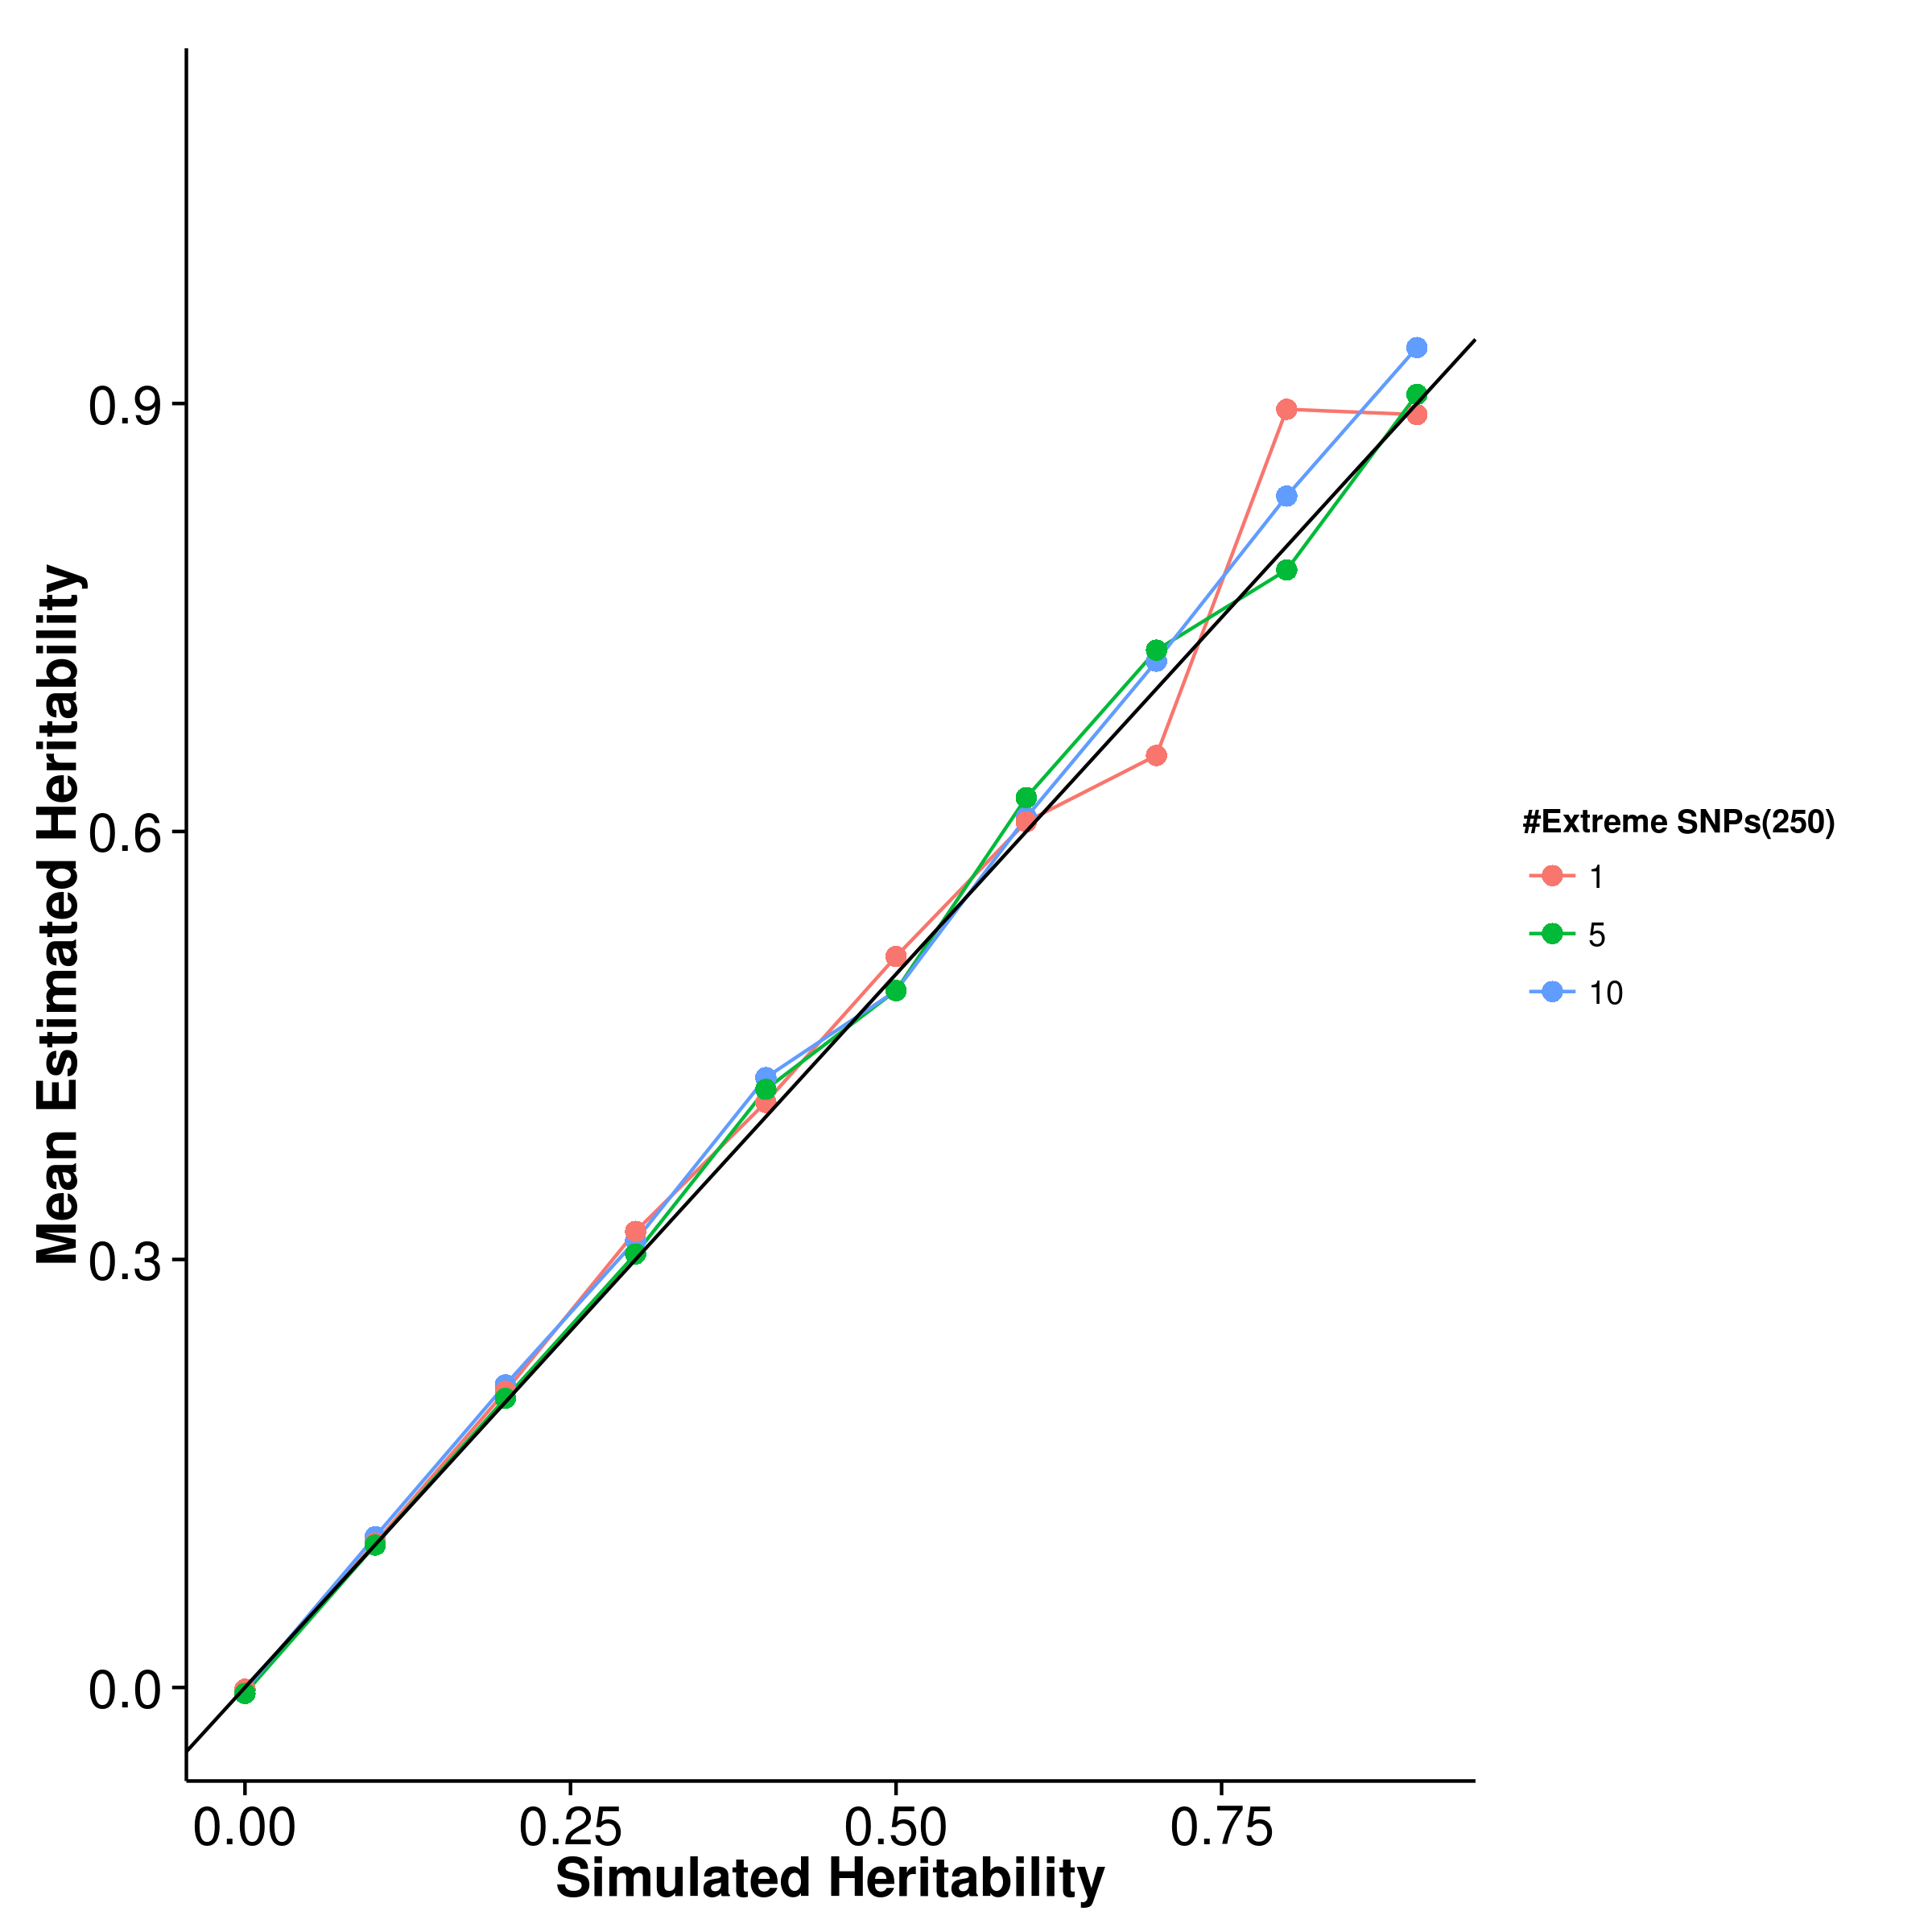
\includegraphics{figure/he_summary/extreme_250c/gcta_QtE_Extreme_mean.png}}
				\label{fig:gctaQtEx250cMean}
			}\\
			\subfloat[LDSC with fix intercept]{
				\scalebox{.4}{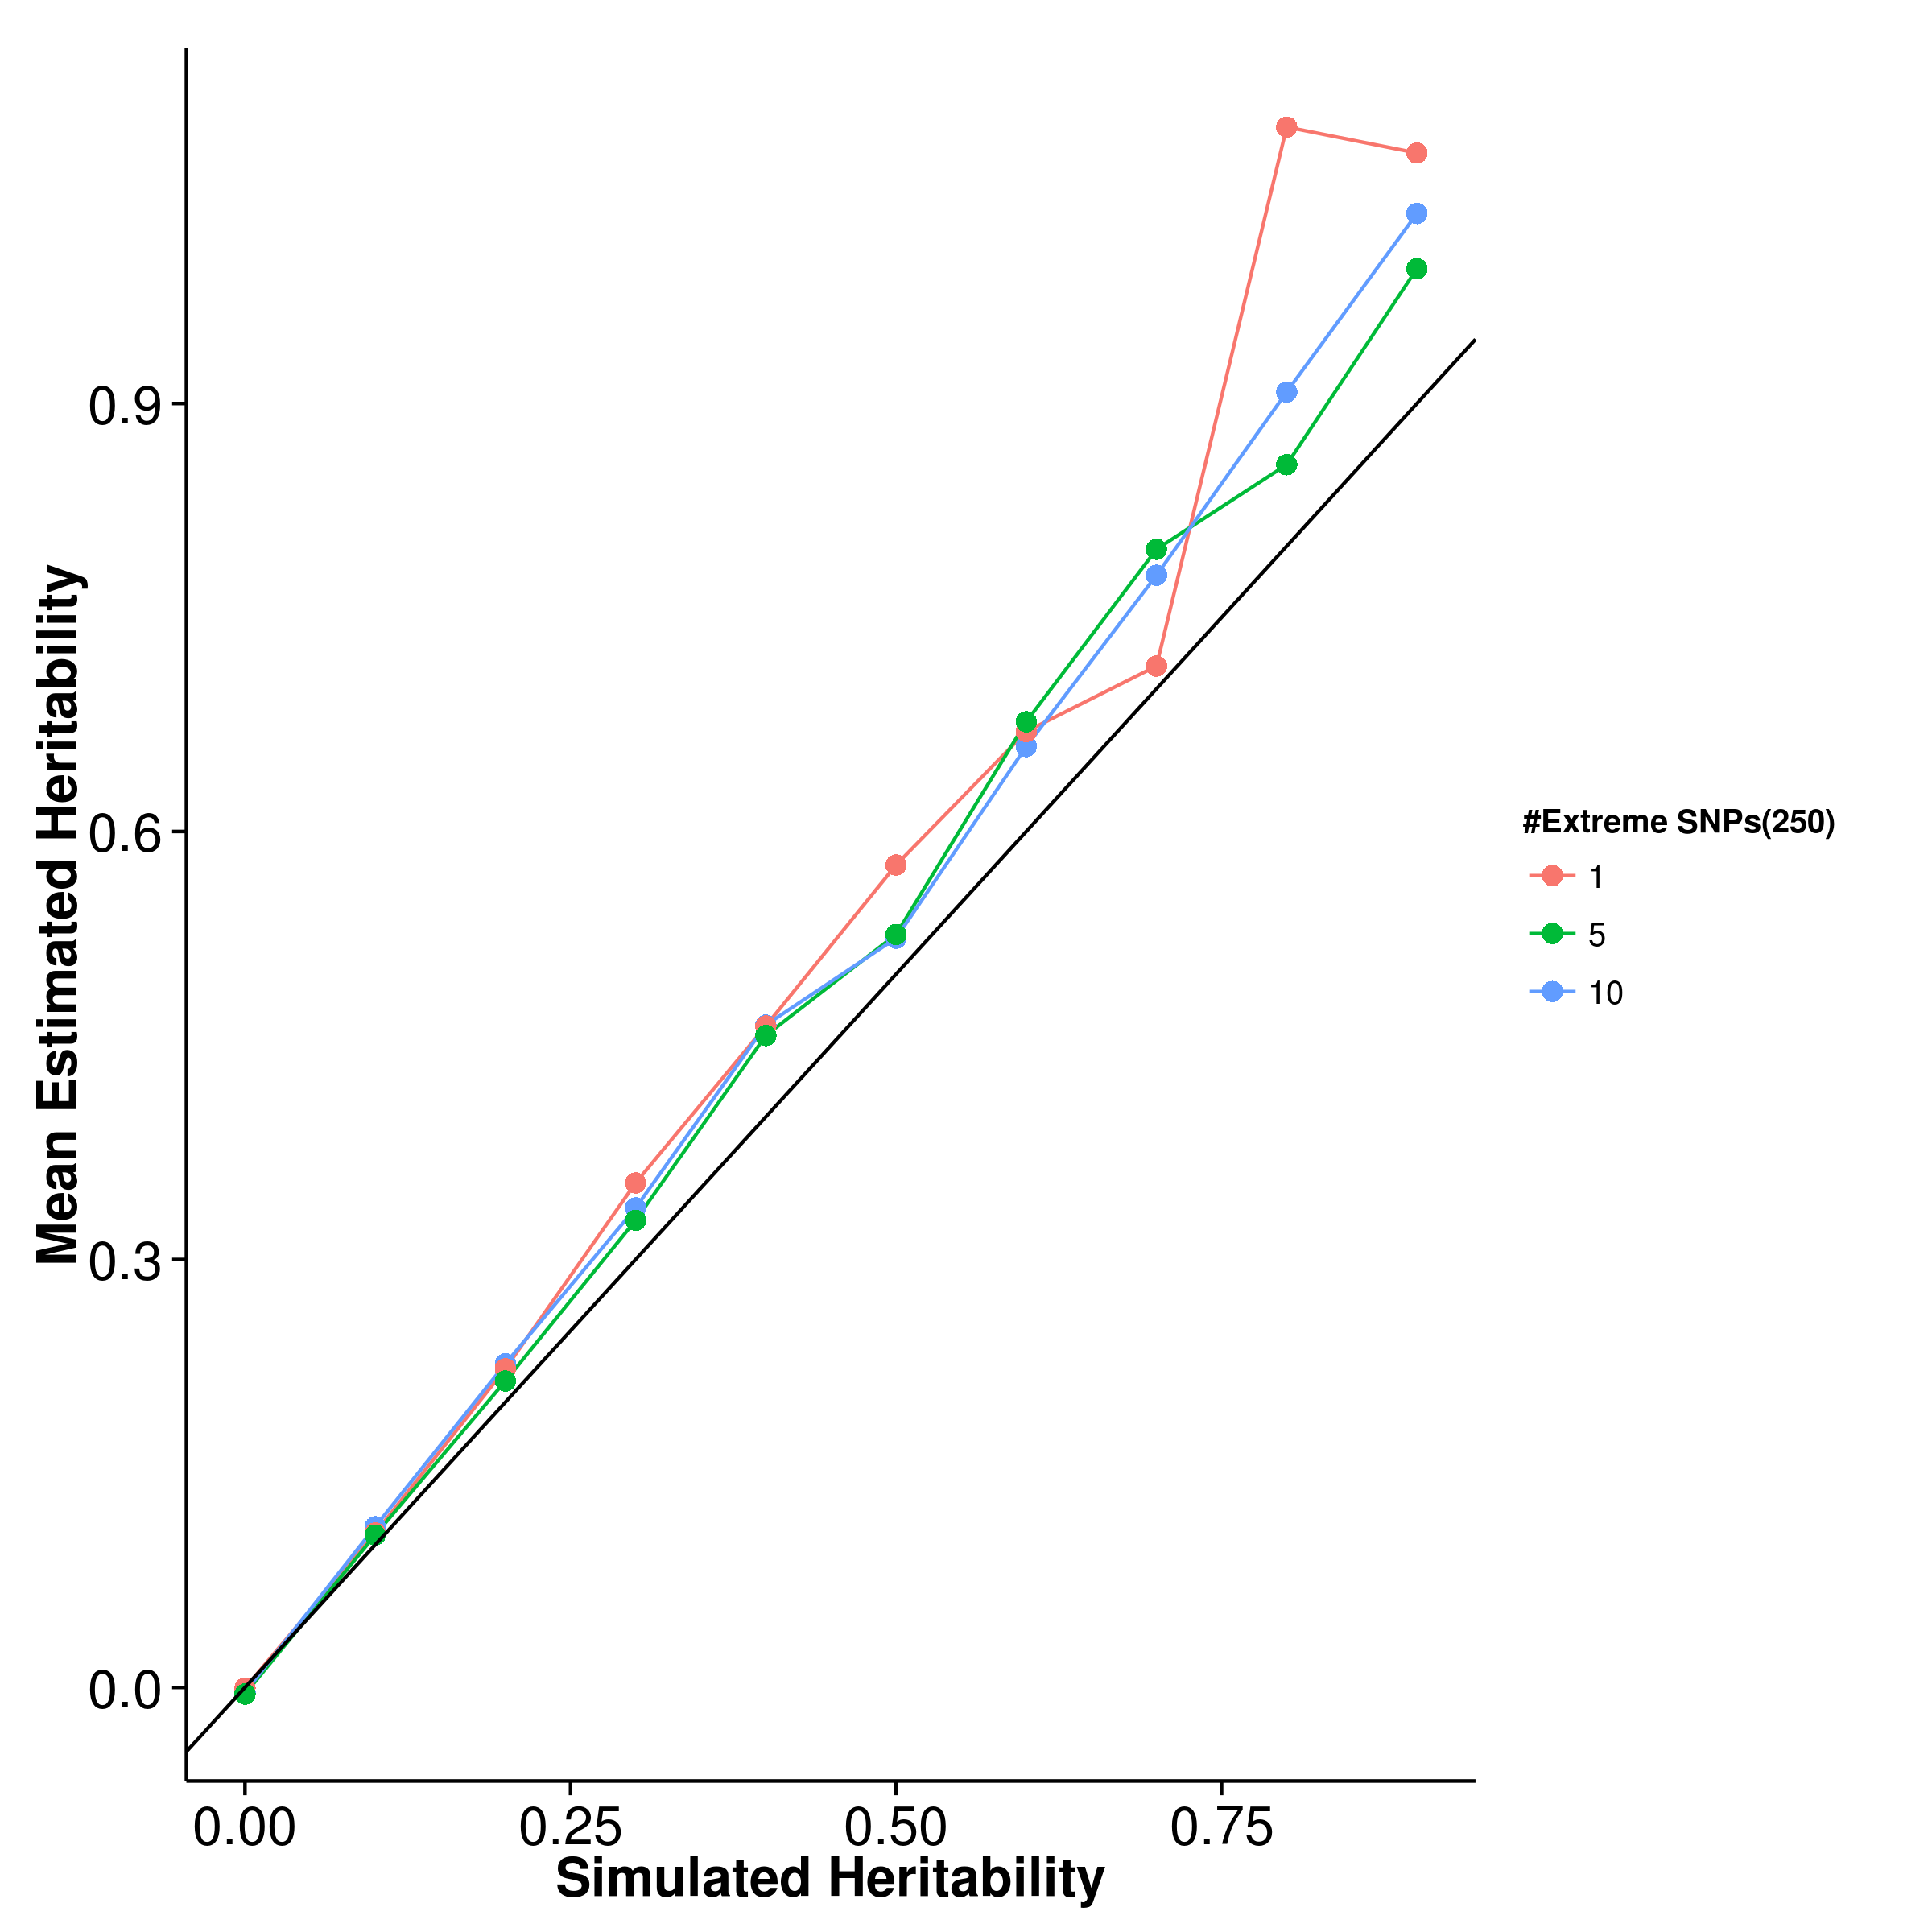
\includegraphics{figure/he_summary/extreme_250c/ldsc_QtE_Extreme_mean.png}}
				\label{fig:ldscQtEx250cMean}
			}
			\subfloat[LDSC with intercept estimation]{
				
				\scalebox{.4}{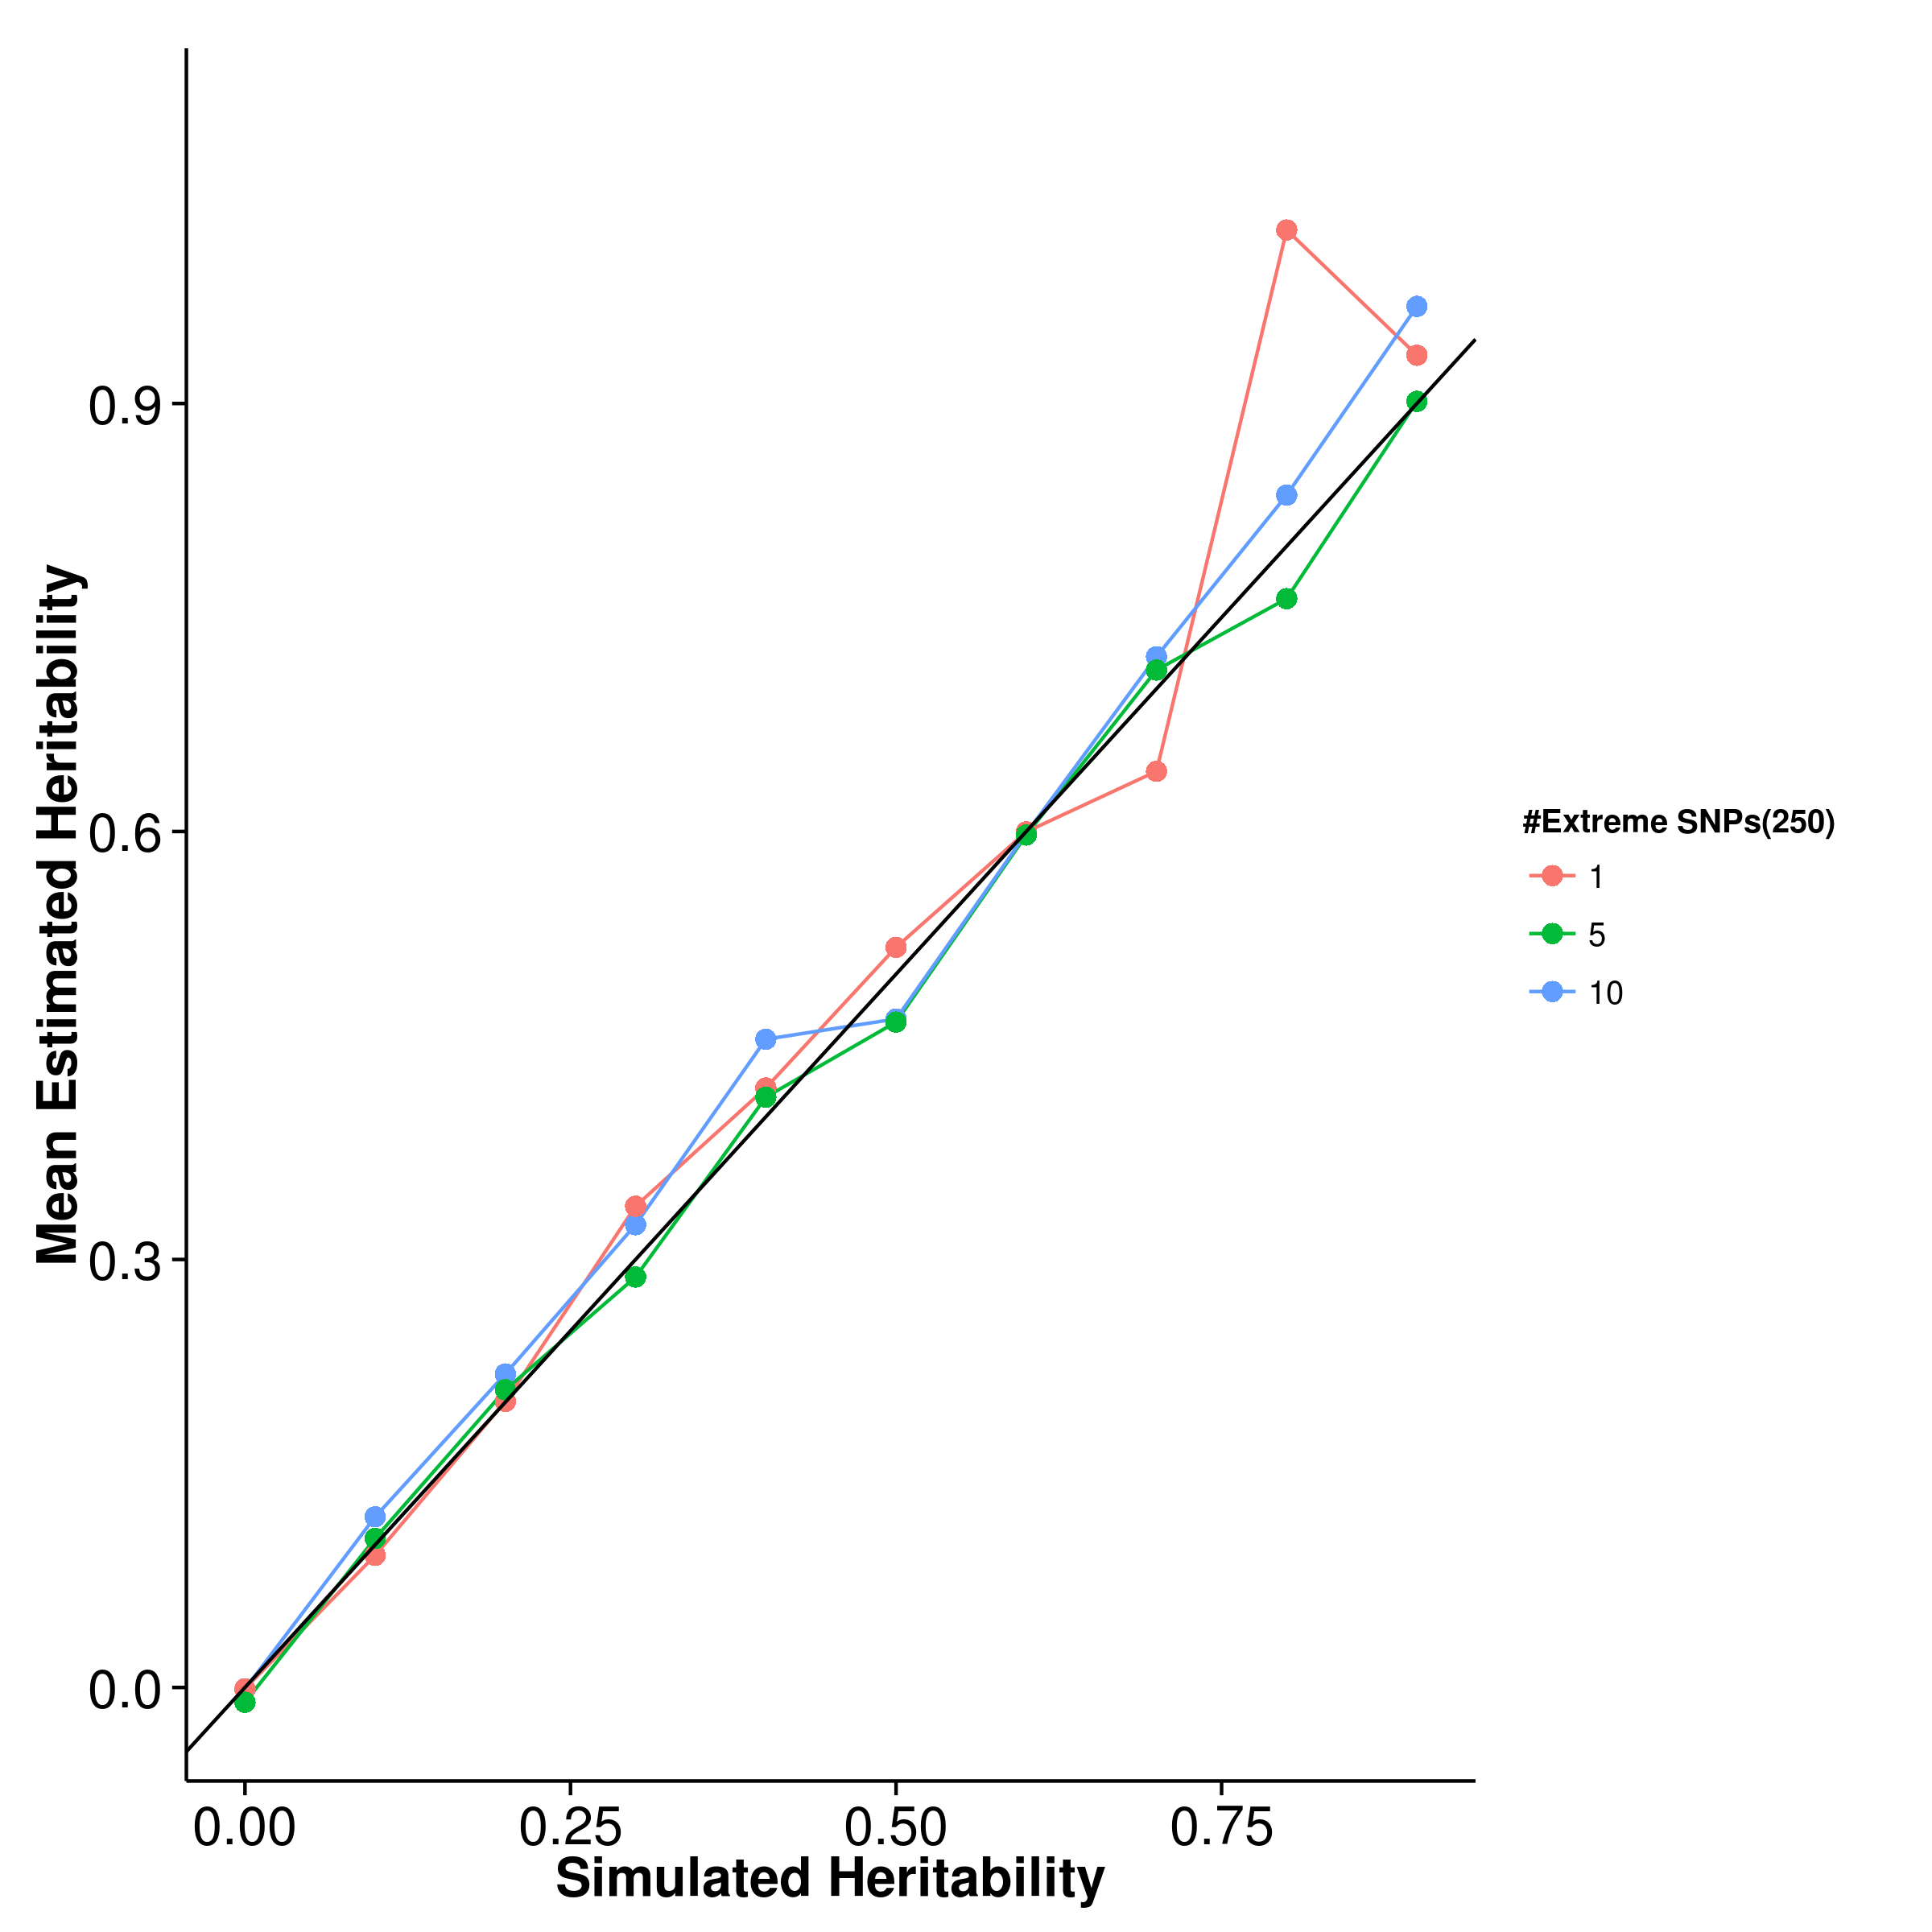
\includegraphics{figure/he_summary/extreme_250c/ldscIn_QtE_Extreme_mean.png}}
				\label{fig:ldscInQtEx250cMean}
			}
			\caption[Quantitative Trait with Extreme Effect Size Simulation Result(250 causal SNPs, Mean)]
			{Mean of results from quantitative trait simulation with extreme effect size simulation.
				250 causal \glspl{SNP} were simulated.
				It was observed that the mean estimation of heritability of all the tools were relatively unaffected by the number of \glspl{SNP} representing a large portion of effect, similar to what observed when 100 causal \glspl{SNP} were simulated.
				However, there seems to be an upward bias when \gls{ldsc} was performed with fixed intercept.
			} 
			\label{fig:QtEx250cMean}
		\end{figure}
		
		\begin{figure}
			\centering
			\subfloat[SHREK]{
				\scalebox{.4}{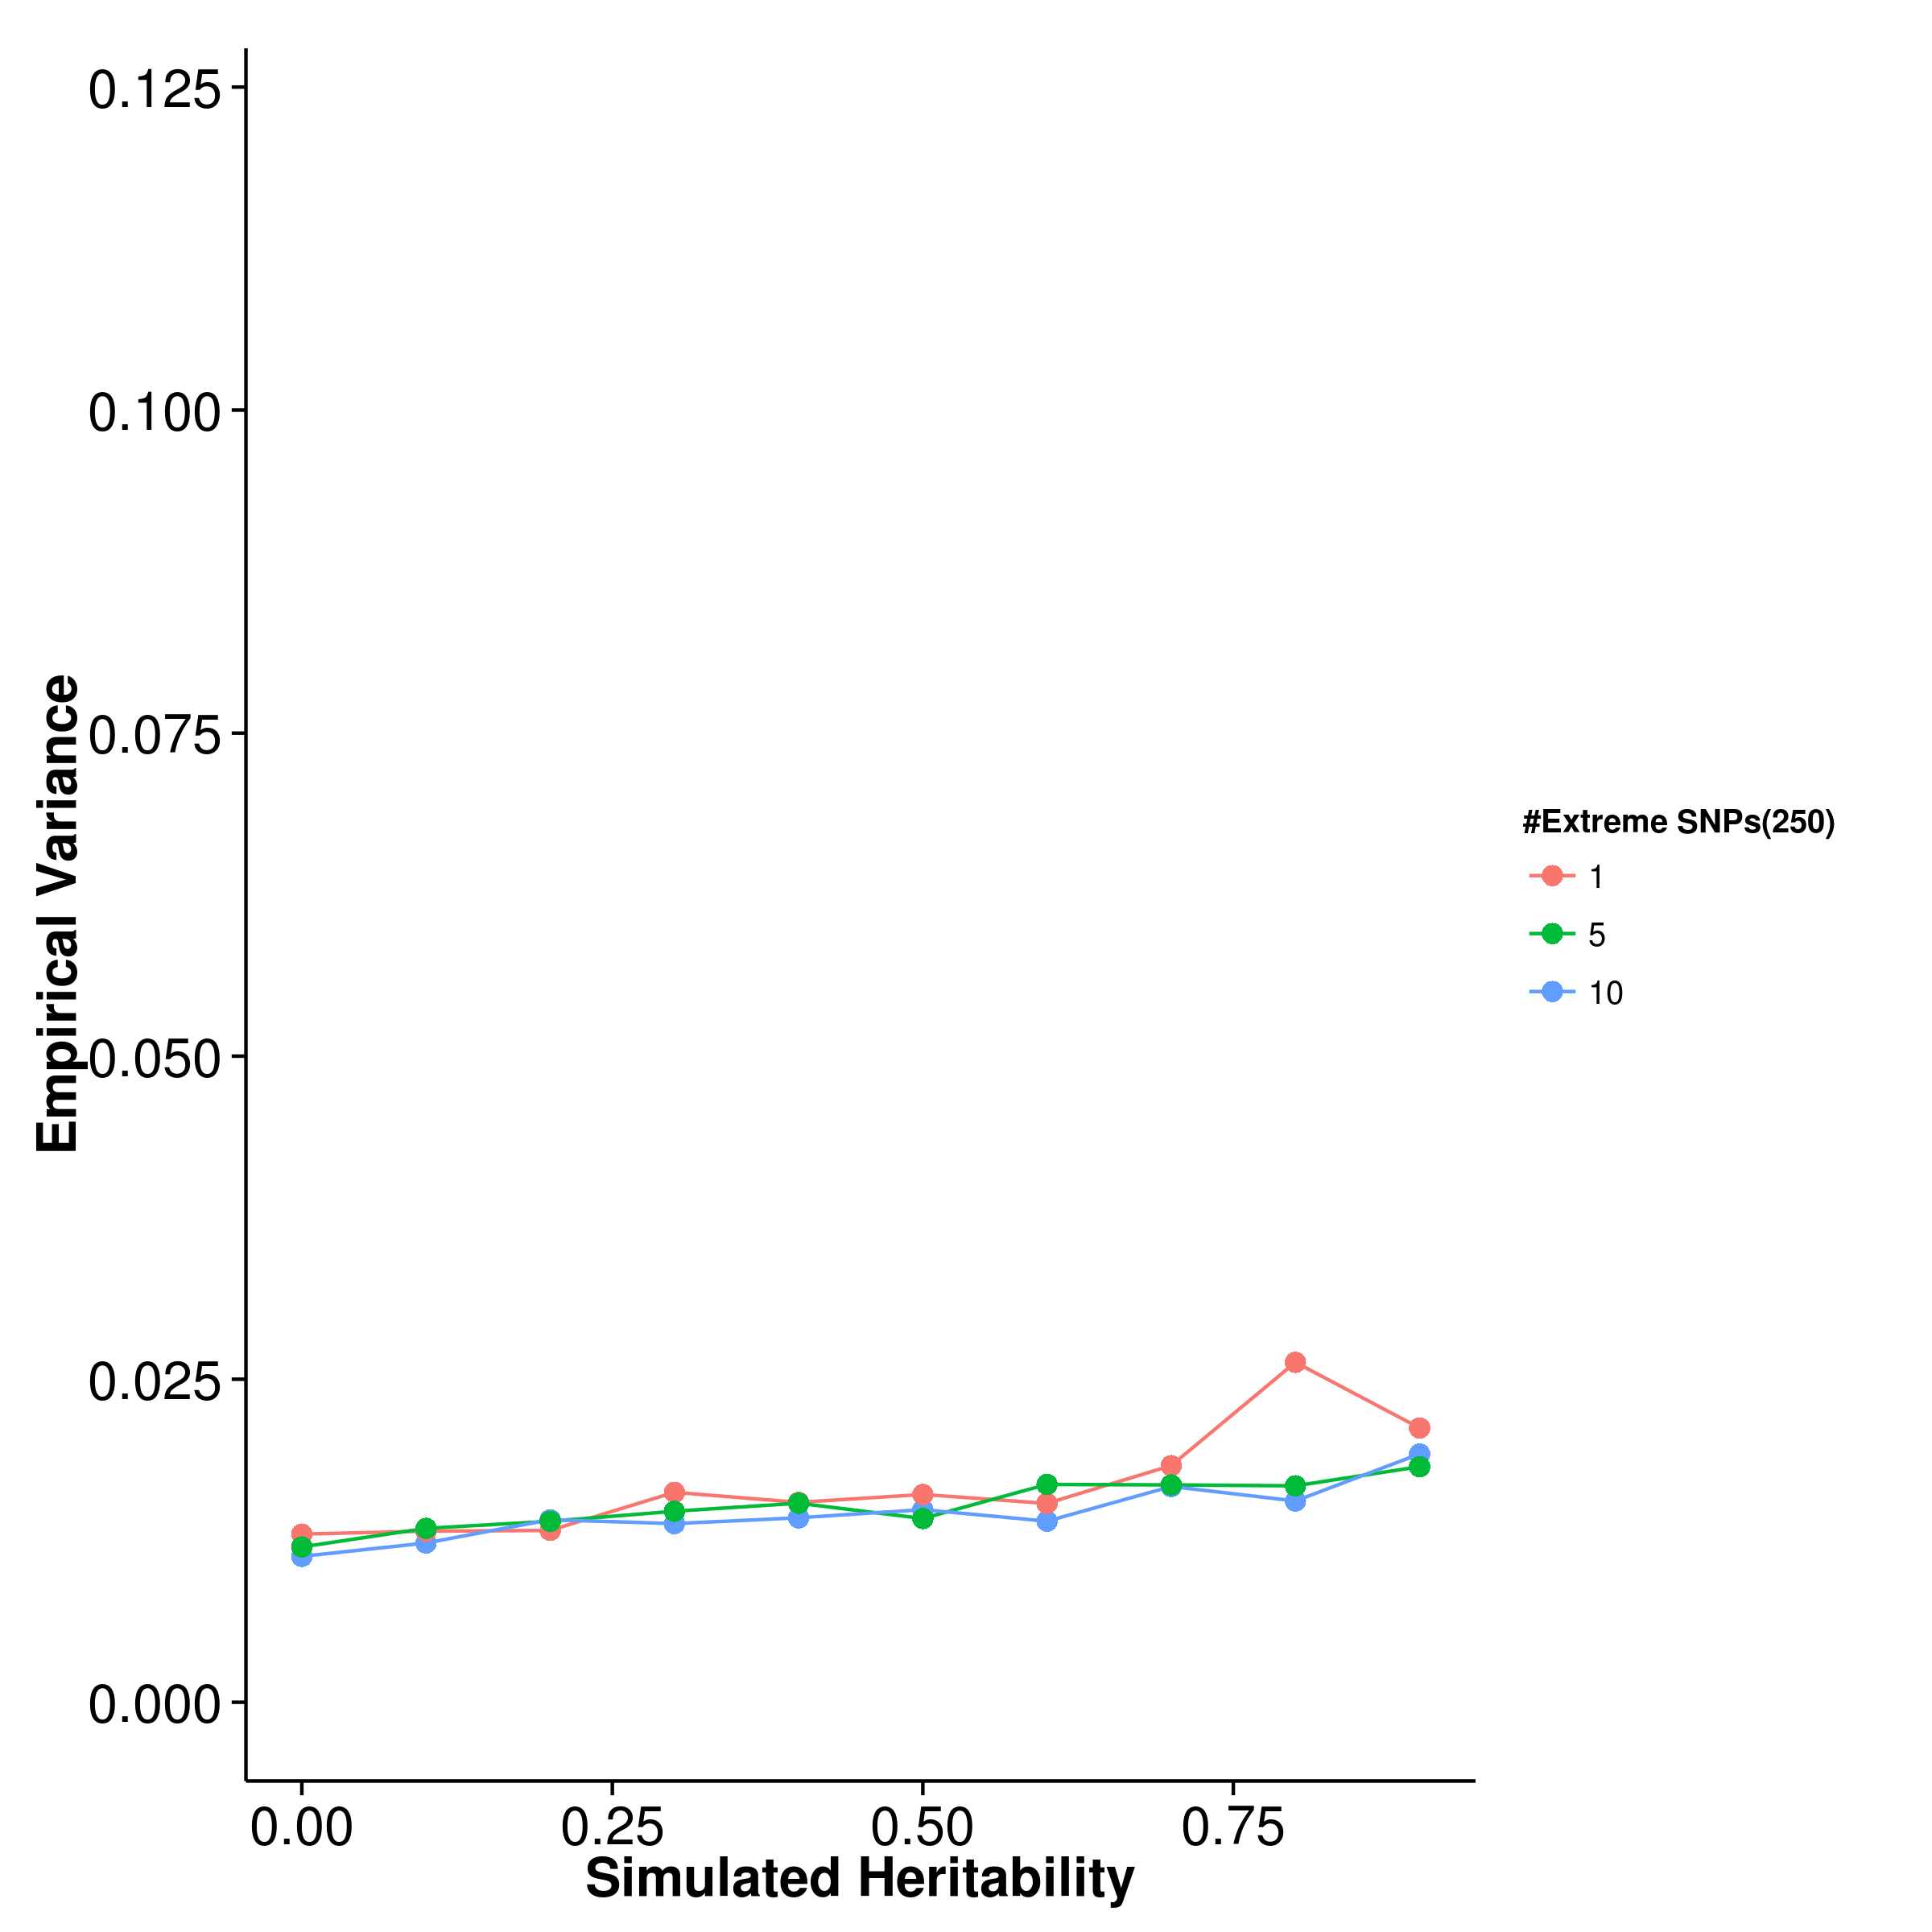
\includegraphics{figure/he_summary/extreme_250c/shrek_QtE_Extreme_sd.png}}
				\label{fig:shrekQtEx250cVar}
			}
			\subfloat[GCTA]{
				\scalebox{.4}{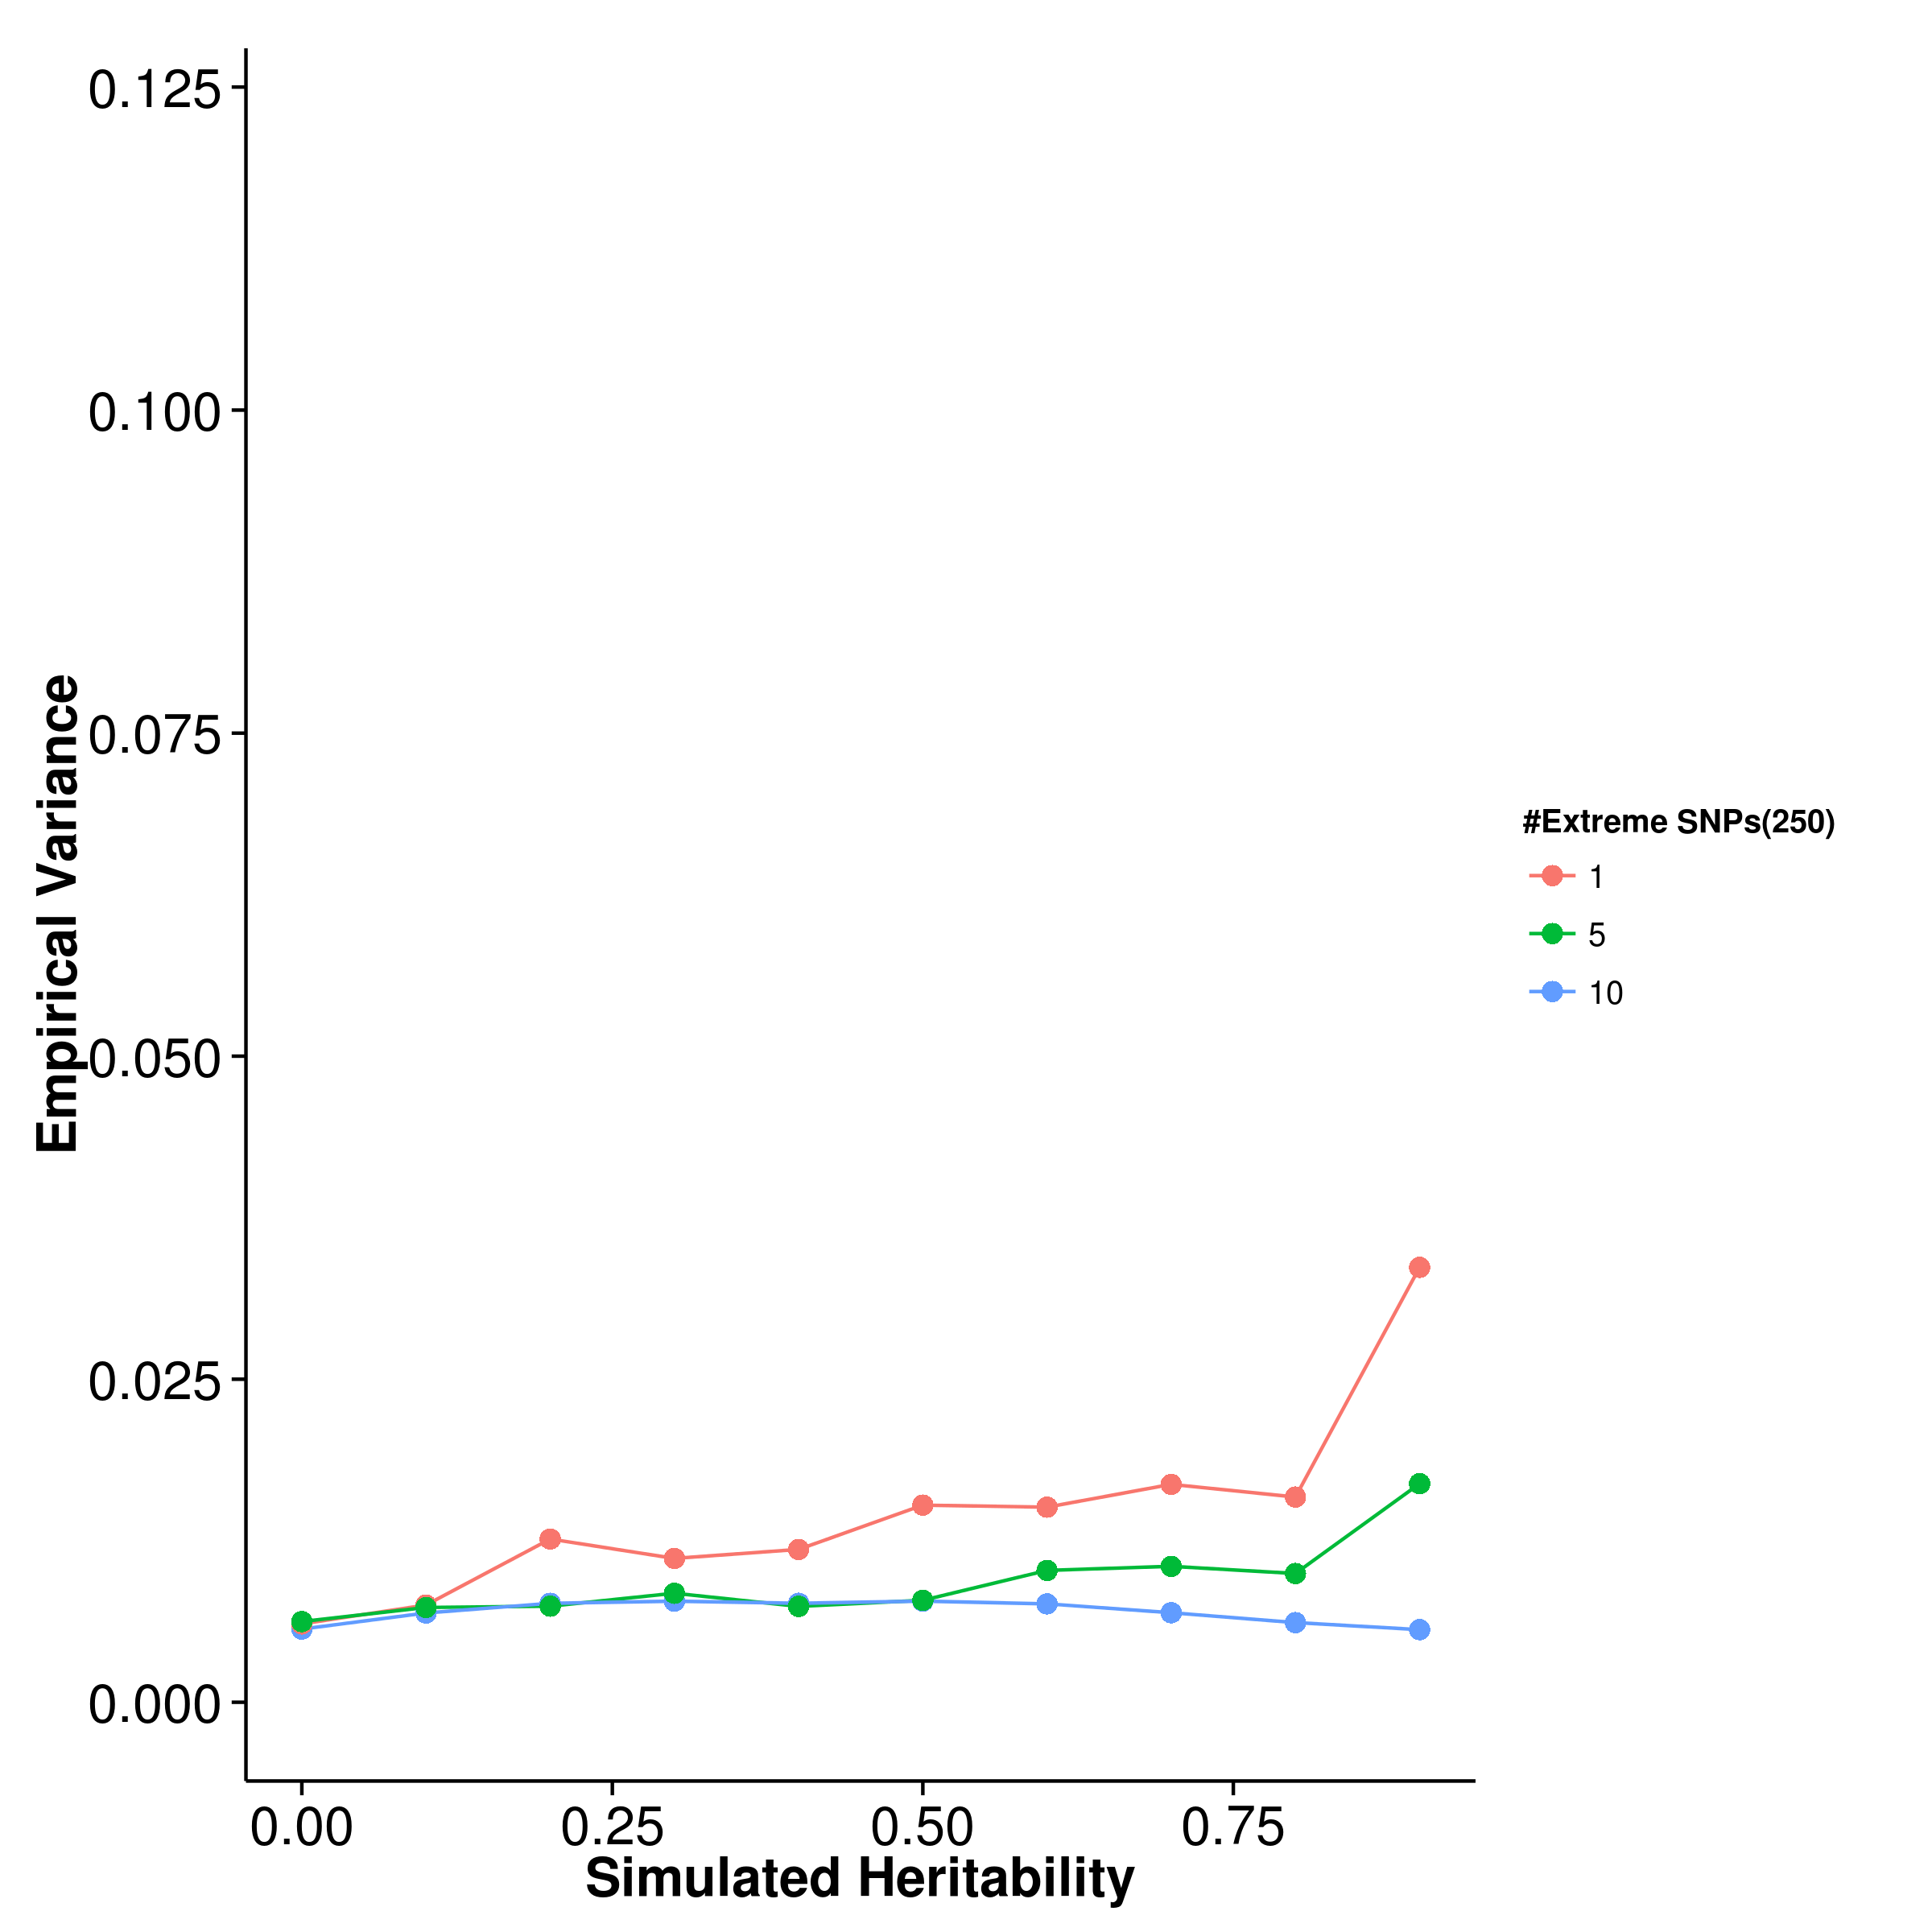
\includegraphics{figure/he_summary/extreme_250c/gcta_QtE_Extreme_sd.png}}
				\label{fig:gctaQtEx250cVar}
			}\\
			\subfloat[LDSC with fix intercept]{
				\scalebox{.4}{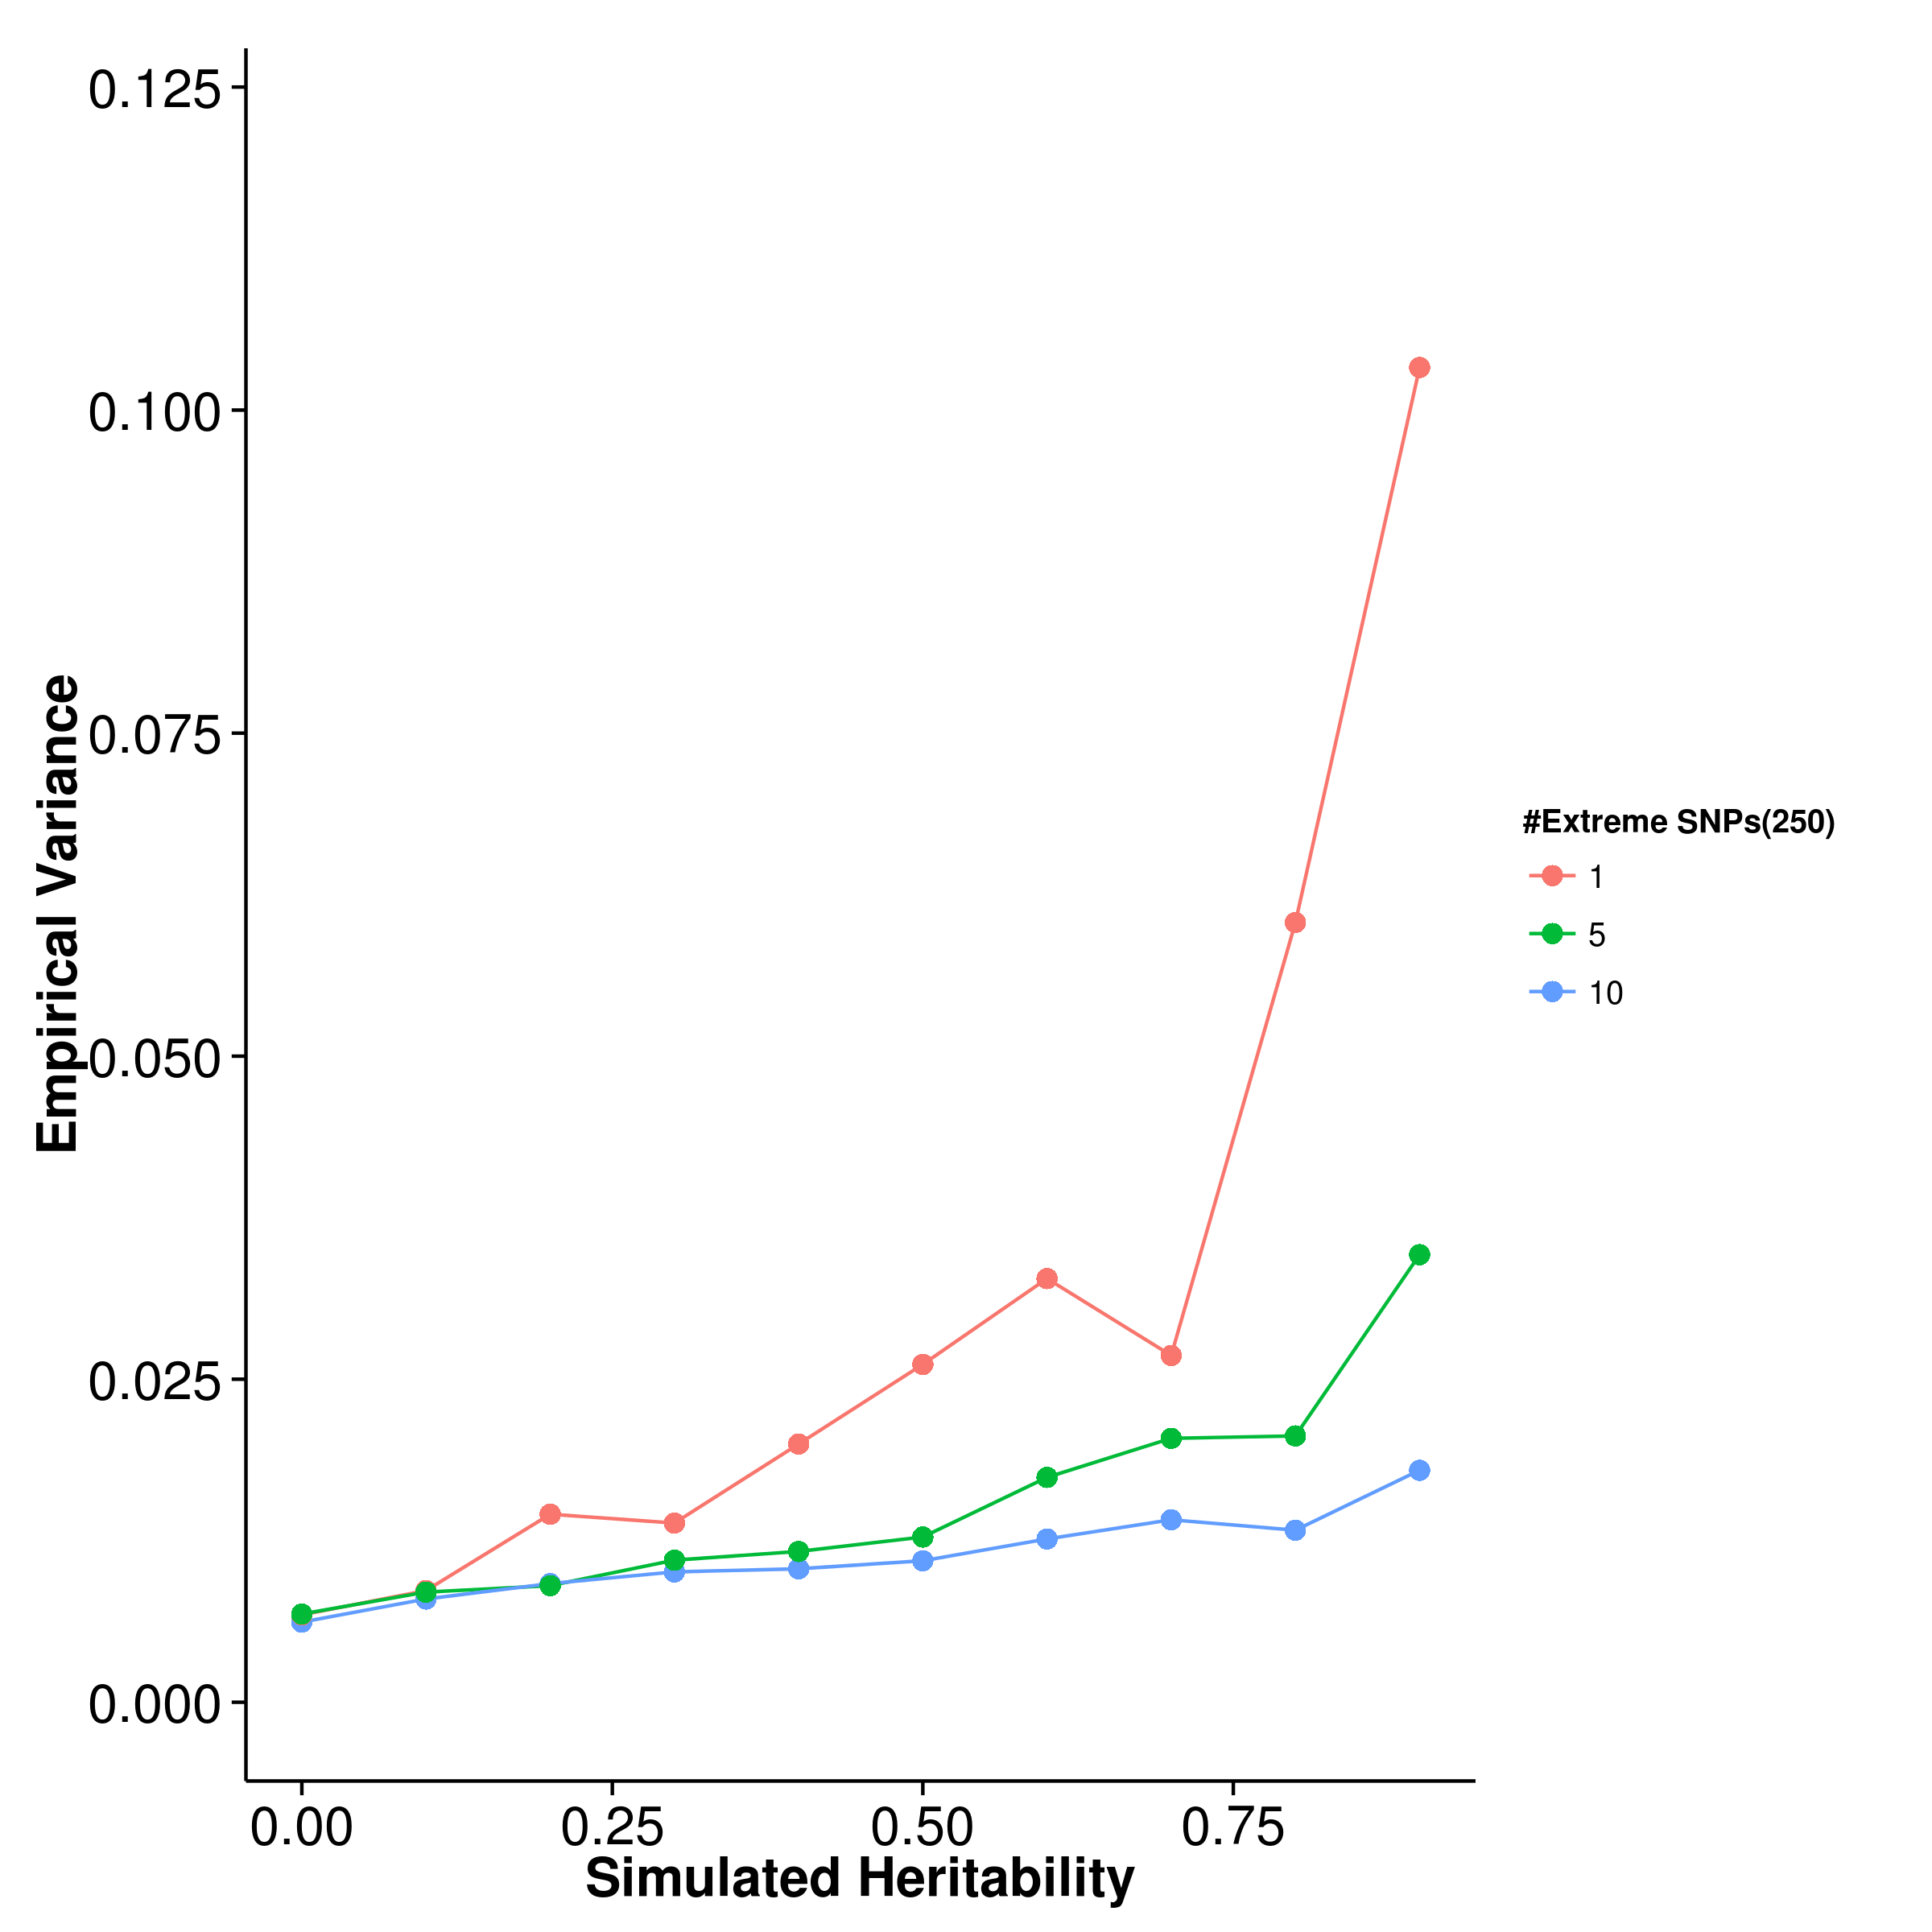
\includegraphics{figure/he_summary/extreme_250c/ldsc_QtE_Extreme_sd.png}}
				\label{fig:ldscQtEx250cVar}
			}
			\subfloat[LDSC with intercept estimation]{
				
				\scalebox{.4}{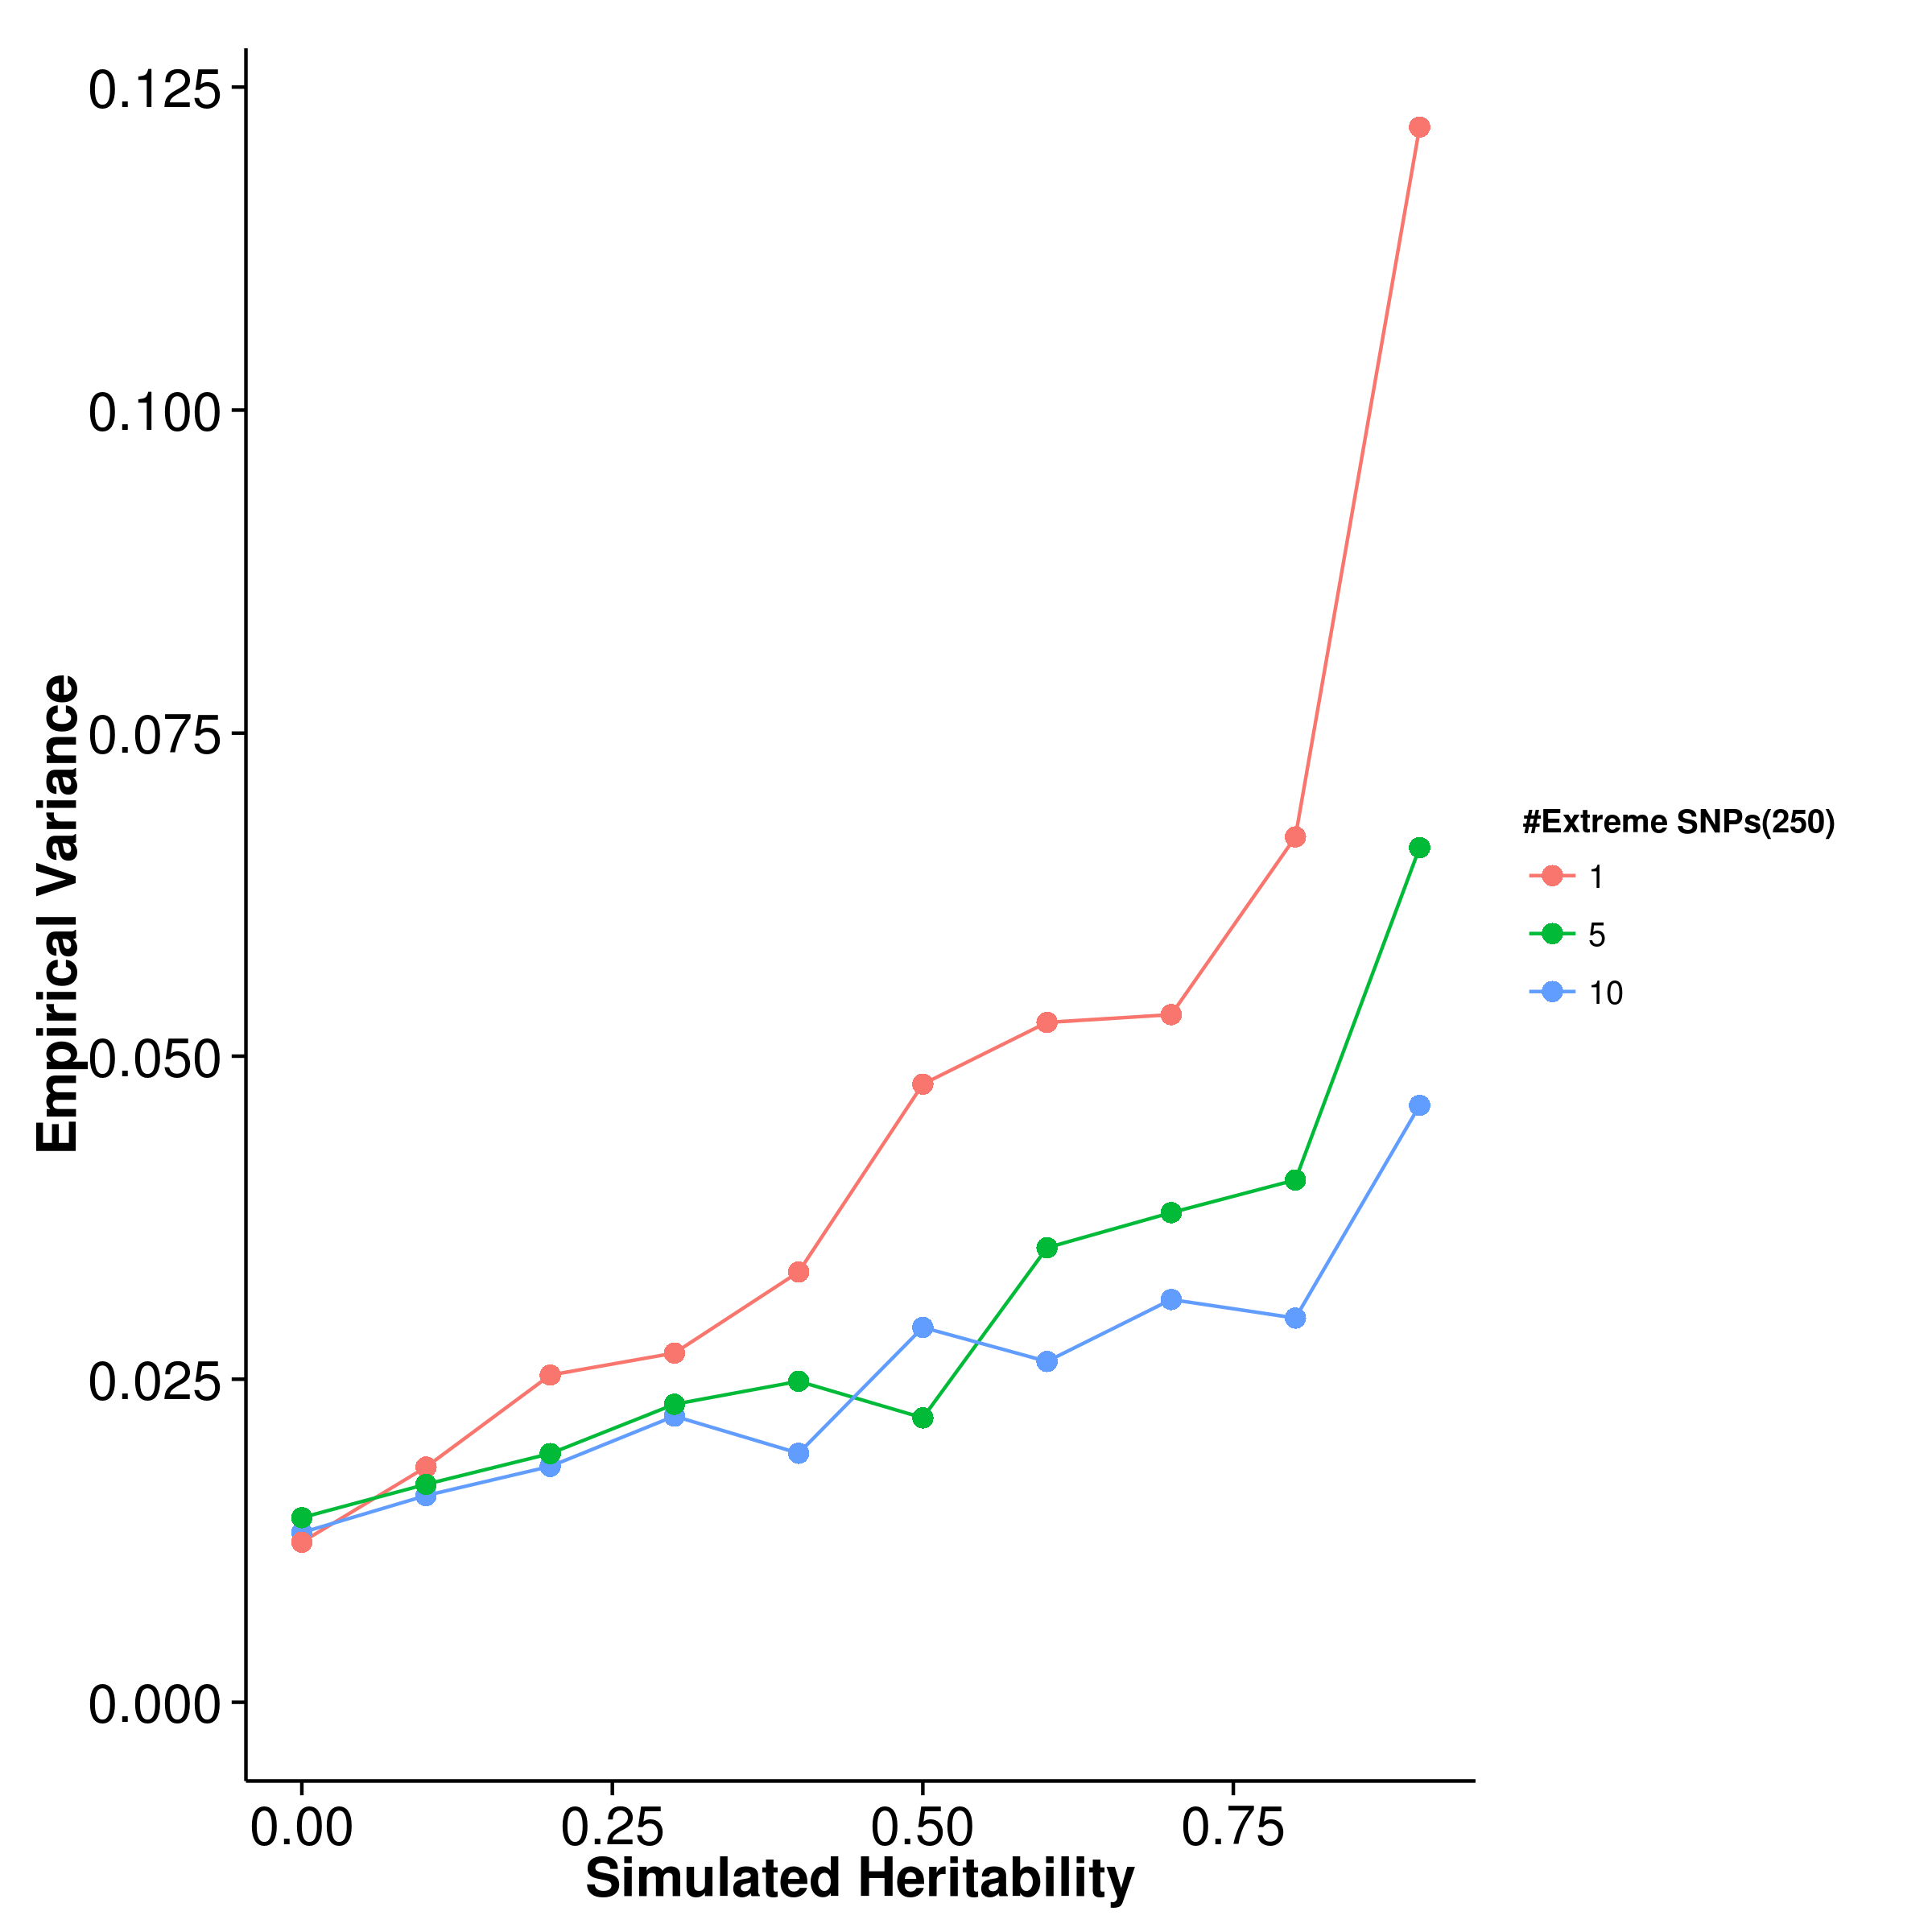
\includegraphics{figure/he_summary/extreme_250c/ldscIn_QtE_Extreme_sd.png}}
				\label{fig:ldscInQtEx250cVar}
			}
			\caption[Quantitative Trait with Extreme Effect Size Simulation Result(250 causal SNPs, Variance)]
			{Variance of results from quantitative trait simulation with extreme effect size simulation.
				250 causal \glspl{SNP} were simulated.
				Compared to the case where 100 causal \glspl{SNP} were simulated, most tools, except \gls{shrek} seems to be more sensitive to the number of \gls{SNP}(s) explaining large portion of effect, where a smaller number can lead to a higher variance.
			} 
			\label{fig:QtEx250cVar}
		\end{figure}
		
		\begin{figure}
			\centering
			\subfloat[SHREK]{
				\scalebox{.4}{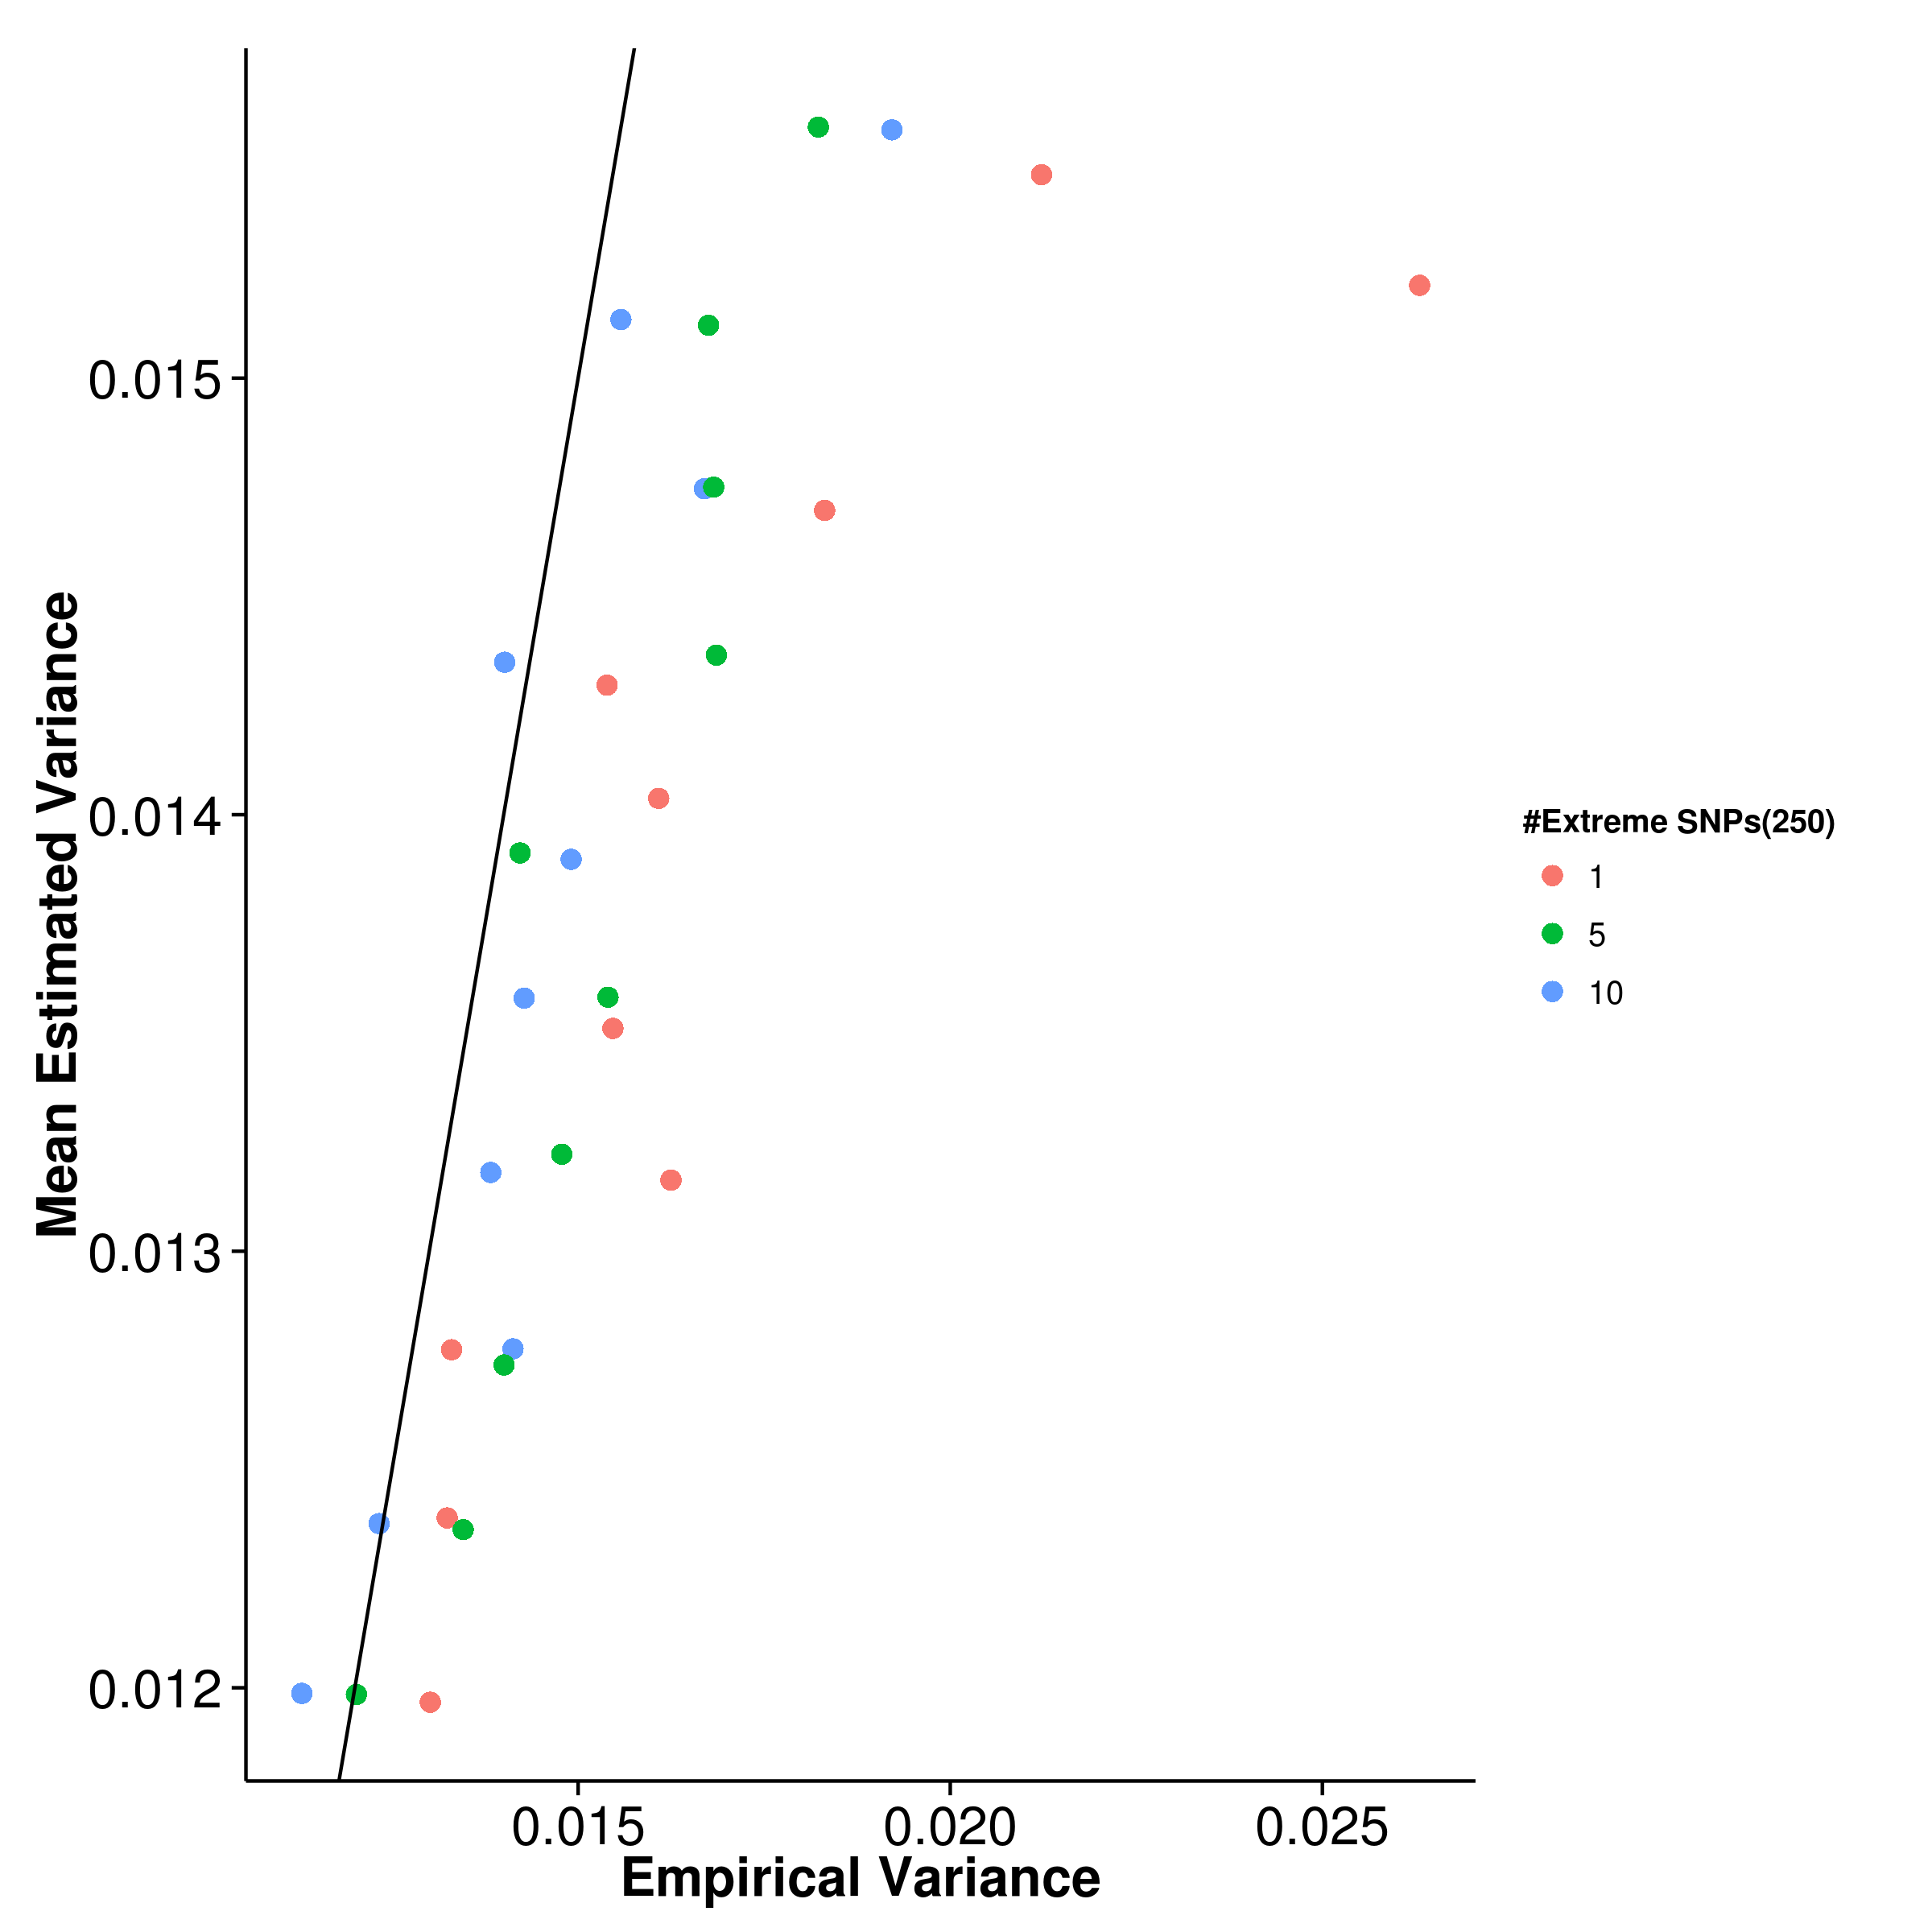
\includegraphics{figure/he_summary/extreme_250c/shrek_QtE_Extreme_sdCom.png}}
				\label{fig:shrekQtEx250cVarCom}
			}
			\subfloat[GCTA]{
				\scalebox{.4}{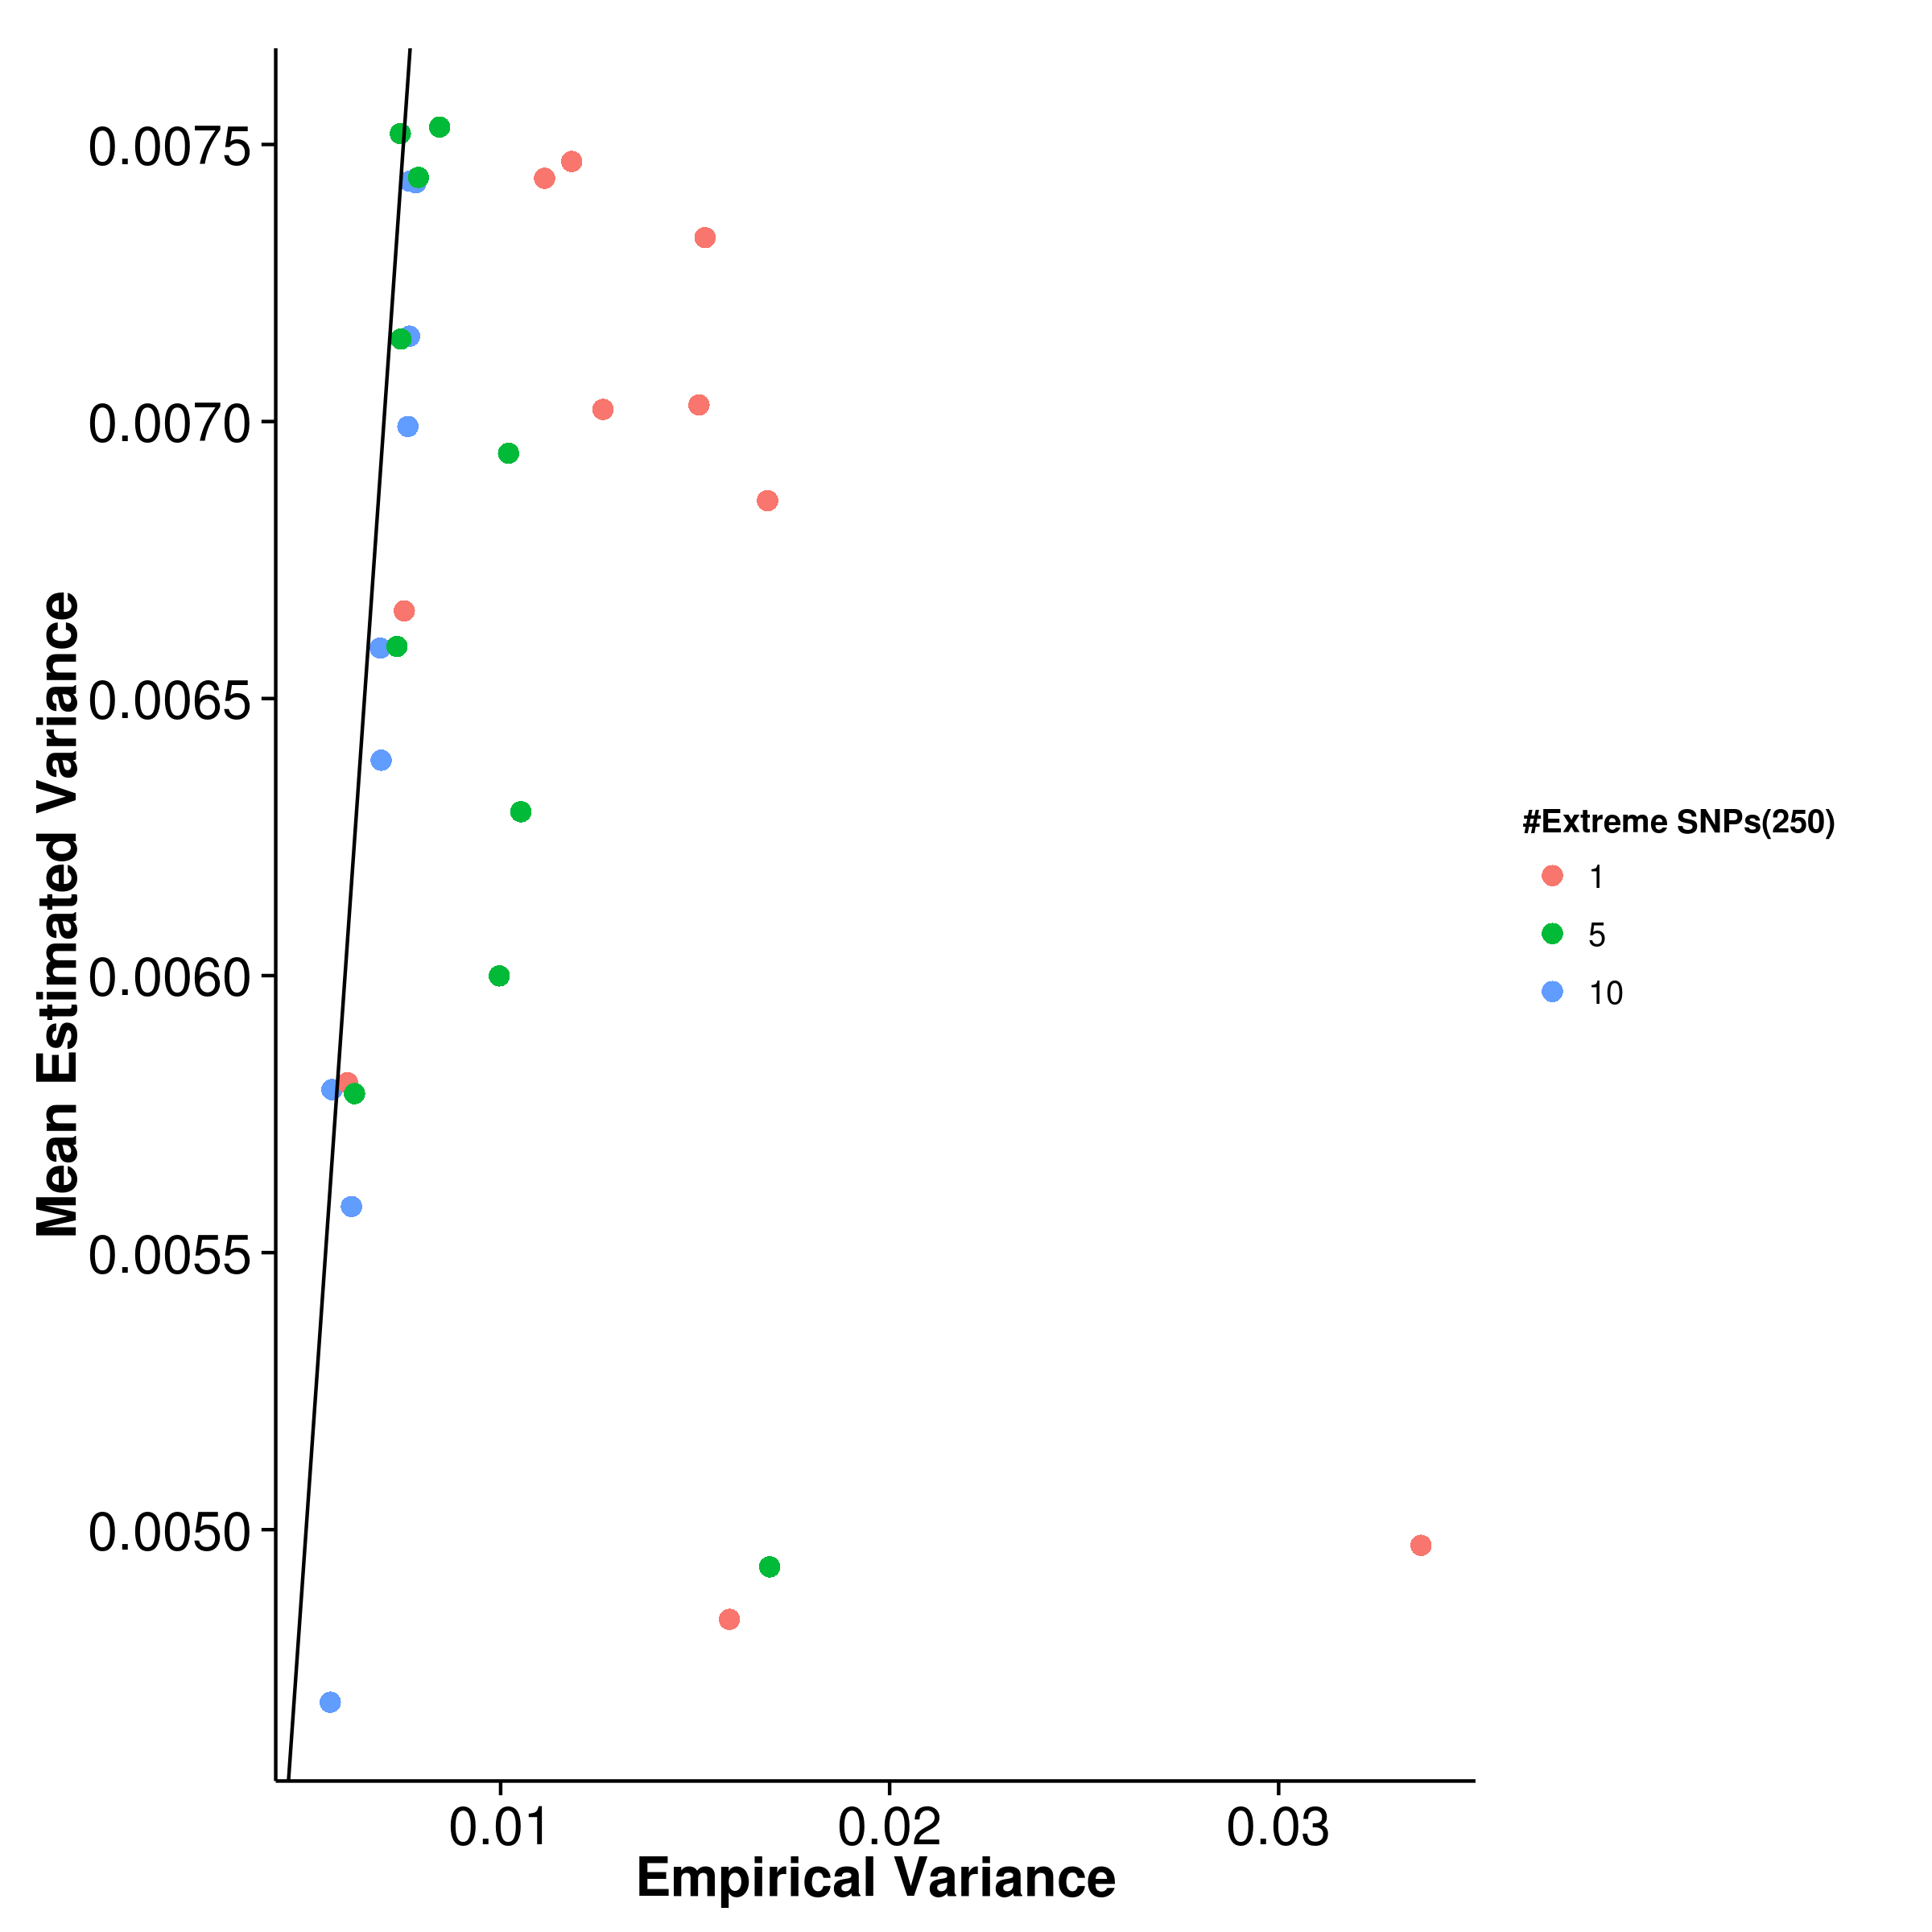
\includegraphics{figure/he_summary/extreme_250c/gcta_QtE_Extreme_sdCom.png}}
				\label{fig:gctaQtEx250cVarCom}
			}\\
			\subfloat[LDSC with fix intercept]{
				\scalebox{.4}{\includegraphics{figure/he_summary/extreme_250c/ldsc_QtE_Extreme_sdCom.png}}
				\label{fig:ldscQtEx250cVarCom}
			}
			\subfloat[LDSC with intercept estimation]{
				
				\scalebox{.4}{\includegraphics{figure/he_summary/extreme_250c/ldscIn_QtE_Extreme_sdCom.png}}
				\label{fig:ldscInQtEx250cVarCom}
			}
			\caption[Quantitative Trait with Extreme Effect Size Simulation Result(250 causal SNPs, Estimated Variance)]
			{Estimated variance of results from quantitative trait simulation with extreme effect size simulation when compared to the empirical variance.
				250 causal \glspl{SNP} were simulated.
				The result of simulation were the same as the previous extreme effect simulation with 100 causal \glspl{SNP}.
			} 
			\label{fig:QtEx250cVarCom}
		\end{figure}
		% CC Rand Effect
		\subsection{Case Control Simulation}
		\begin{figure}
			\centering
			\subfloat[SHREK]{
				\scalebox{.4}{\includegraphics{figure/he_summary/cc_100c/shrek_CC_Random_mean.png}}
				\label{fig:shrekCCRandMean}
			}
			\subfloat[GCTA]{
				\scalebox{.4}{\includegraphics{figure/he_summary/cc_100c/gcta_CC_Random_mean.png}}
				\label{fig:gctaCCRandMean}
			}\\
			\subfloat[LDSC with fix intercept]{
				\scalebox{.4}{\includegraphics{figure/he_summary/cc_100c/ldsc_CC_Random_mean.png}}
				\label{fig:ldscCCRandMean}
			}
			\subfloat[LDSC with intercept estimation]{
				
				\scalebox{.4}{\includegraphics{figure/he_summary/cc_100c/ldscIn_CC_Random_mean.png}}
				\label{fig:ldscInCCRandMean}
			}
			\caption[Case Control with Random Effect Size Simulation Result(Mean)]
			{Mean of results from case control simulation with random effect size simulation.
				The performance of \gls{gcta} was as suggested by \citet{Golan2014} where there was an underestimation as prevalence decreases.
				On the other hand, \gls{ldsc} were upwardly biased when a fixed intercept was used and this bias was corrected when an estimation of intercept was allowed.
				\gls{shrek} does not seems to as sensitive to change in prevalence and the estimation were relatively robust.
				} 
			\label{fig:CCRandMean}
		\end{figure}
		
		\begin{figure}
			\centering
			\subfloat[SHREK]{
				\scalebox{.4}{\includegraphics{figure/he_summary/cc_100c/shrek_CC_Random_sd.png}}
				\label{fig:shrekCCRandVar}
			}
			\subfloat[GCTA]{
				\scalebox{.4}{\includegraphics{figure/he_summary/cc_100c/gcta_CC_Random_sd.png}}
				\label{fig:gctaCCRandVar}
			}\\
			\subfloat[LDSC with fix intercept]{
				\scalebox{.4}{\includegraphics{figure/he_summary/cc_100c/ldsc_CC_Random_sd.png}}
				\label{fig:ldscCCRandVar}
			}
			\subfloat[LDSC with intercept estimation]{
				
				\scalebox{.4}{\includegraphics{figure/he_summary/cc_100c/ldscIn_CC_Random_sd.png}}
				\label{fig:ldscInCCRandVar}
			}
			\caption[Case Control with Random Effect Size Simulation Result(Variance)]
			{Variance of results from case control simulation with random effect size simulation.
				It was clear that the prevalence affects the variance of estimation where a larger variance tends to increase the variance of estimation.
				Again, \gls{gcta} has the lowest variance, however, unlike in the quantitative trait simulation, \gls{shrek} has a lower average variance when compared to \gls{ldsc} with fixed intercept.
				Nonetheless, it was important to remember that in case control simulation, a much smaller amount of \glspl{SNP} was used, thus the results was not directly comparable to results from the quantitative simulation.
			} 
			\label{fig:CCRandVar}
		\end{figure}
		
		
		\begin{figure}
			\centering
			\subfloat[SHREK]{
				\scalebox{.4}{\includegraphics{figure/he_summary/cc_100c/shrek_CC_Random_sdCom.png}}
				\label{fig:shrekCCRandVarCom}
			}
			\subfloat[GCTA]{
				\scalebox{.4}{\includegraphics{figure/he_summary/cc_100c/gcta_CC_Random_sdCom.png}}
				\label{fig:gctaCCRandVarCom}
			}\\
			\subfloat[LDSC with fix intercept]{
				\scalebox{.4}{\includegraphics{figure/he_summary/cc_100c/ldsc_CC_Random_sdCom.png}}
				\label{fig:ldscCCRandVarCom}
			}
			\subfloat[LDSC with intercept estimation]{
				
				\scalebox{.4}{\includegraphics{figure/he_summary/cc_100c/ldscIn_CC_Random_sdCom.png}}
				\label{fig:ldscInCCRandVarCom}
			}
			\caption[Case Control with Random Effect Size Simulation Result(Estimated Variance)]
			{Estimated variance of results from case control simulation with random effect size simulation when compared to empirical variance.
				From the quantitative trait simulation with random effect size(\cref{fig:QtRandVarCom}), it was observed that the variance estimation of \gls{shrek} and \gls{gcta} were rater accurate.
				Similarly, in the case control simulation with 100 causal \glspl{SNP}, it was observed that the variance estimation of \gls{shrek} and \gls{gcta} were close to the empirical variance with slight bias.
				A large up-ward bias was observed for \gls{ldsc} with fixed intercept estimation but the bias was less when \gls{ldsc} was allowed to estimate the intercept.s
			} 
			\label{fig:CCRandVarCom}
		\end{figure}
		
		
		
		
	\section{Discussion}
	
	\section{Supplementary place holder}

	
	%Put these graphs in supplementary instead
	
	\chapter{Heritability of Schizophrenia}
	\section{Introduction}
	Apply Heritability estimation to the schizophrenia data.
	The genetic correlation and partitioning of heritability
	No one worked on linking schizophrenia with brain development directly?
	% talk about the current research on schizophrenia?
	% the overall heritablity estimation
	% The genetic correlation done by the LDSC. 
	% The theory of brain development 
	% How the co-expression network works
	% Drug response?
	\section{Heritability Estimation}
	This will be a very simple section, focused on how to perform the heritability estimation on \acrfull{scz}.
	Should also tokenize the heritability into subcategories (e.g. immune, neuron, etc)
	%Should not put too much weight into it, otherwise it will be a direct copy of LDSC. Won't really add much power. 
	
	
	\subsection{Methodology}
	\subsection{Result}
	\section{Brain development and Schizophrenia}
	\sectionmark{Brain development}
	Here we will perform the WGCNA and brain development network.
	Seeing how the whether if any brain development network were enriched with SNPs that explain the variance of phenotype
	%Instead, we should put most focus here as no one has done it before
	%Also descript brainspan here
	\subsection{Methodology}
	\subsubsection{Sample Quality Controls}
	We obtain the developmental transcriptome data from BrainSpan (\url{http://www.brainspan.org/}). 
	A total of 56 samples with different age were provided by BrainSpan with an average of 2.2 samples per age.
	
	Studies suggested Hippocampus\citep{Velakoulis2006,Nugent2007}, Amygdala and Striatum\citep{Simpson2010} are brain regions involved in the etiology of schizophrenia. 
	Therefore, we focus on building the gene co-expression network of hippocampus, amygdala and striatum in this study
	It is worth noting that the Pre-frontal Cortex is also important for schizophrenia. 
	However, as there isn't a well defined pre-frontal cortex samples from BrainSpan, we did not include the pre-frontal cortex in the current study.
	RNA Sequencing data of the brain regions were obtained from BrainSpan and undergo a series of quality control before the construction of the network. 
	 
	For each sample age, when there are more than one samples, we select the sample with a dissection score $\ge3$ and an \gls{rin} $\ge7$. 
	As some developmental stage only got 1 sample passing the quality check, we limit each developmental stage to have a maximum of 1 sample such that the final network will not be driven by a particular developmental stage. 
	If multiple samples passed through the quality check threshold, we will prefer sample with higher dissection score. 
	Shall multiple samples have the same dissection score, we will select the one with the highest \gls{rin}. 
	And if the samples have the same dissection score and \gls{rin} value, we will randomly select one for the network construction.
	
	After performing the quality control, a total of 16, 18 and 15 samples were selected for hippocampus, amygdala and striatum respectively.
	The sample age ranged from \gls{gd}8 to 23 years old representing the fetal developmental stage till the age of onset of schizophrenia.
	
	\subsubsection{Normalization of data}
	The RNA Sequencing data were represented as \gls{rpkm} values. 
	Genes with a low \gls{rpkm} can usually be a result from technical or biological noise\citep{Hart2013}.
	To reduce noise in the final model, genes with a mean \gls{rpkm} $< 1$ in all samples were discarded. 
	The \gls{rpkm} were then log transformed as instructed by the manual of \gls{wgcna}\citep{Langfelder2008}.
	
	As there are insufficient samples for the construction of gene co-expression network for individual sample age, we try to construct networks with genes co-expressed through all sample stage. 
	This is achieved by taking the standardized log$_2$ \gls{rpkm} across sample age such that all genes has a mean of 0 and standard deviation of 1.
	
	At the end, there were 17,168 genes, 17,038 genes and 17,166 genes passing through the quality threshold and were used for the construction of co-expression network in hippocampus, amygdala and striatum respectively. 
	 
	\subsubsection{Network Construction}
	\gls{wgcna} (ver 1.47) were used for the construction of gene co-expression network\citep{Langfelder2008}. 
	The \emph{blockwiseModules} function, using Biweight Midcorrelation for the construction of correlation matrix and a restriction of minimum network size of 30. 
	For the construction of gene co-expression networks in hippocampus, the soft-power threshold were set to 15 where it is the first threshold value which has $R^2 > 0.8$ (0.817) and the $R^2$ is saturated\citep{Zhang2005}.%(\cref{fig:softpowerThreshold})
	As for striatum, the soft-power threshold were set to 20. 
	Again, this is the first threshold value with $R^2 >0.8$ (0.879) and where the $R^2$ is saturated.
	
	On the other hand, for amygdala, soft-power threshold were set to 9 which is the first threshold for $R^2$ to reach saturation. 
	However, with a soft-power threshold of 9, the $R^2$ were only 0.776, which is lower than the recommended 0.8 threshold.
	The reason behind this decision was that the first soft-power threshold to have $R^2 > 0.8$ is 30.
	Under this threshold, the mean connectivity of the resulting networks will be around 23.6 with a median connectivity of 2.51.
	Such level of connectivity will likely yield networks that are too small to useful.
	If one would like to satisfy both requirement of threshold selection, a threshold $>30$ are likely required and any networks constructed will likely to be small.
	As a result of that, we select threshold of 9 where networks with reasonable size can be constructed.
	
	%\begin{figure}
	%	\caption[Soft-power threshold selection]{Soft-power threshold selection. A soft-power of 13 were selected as it is the first threshold value having $R^2 > 0.8$ (0.817) and where the $R^2$ is saturated.}
	%	\centering
	%	\scalebox{.8}{\includegraphics{figure/SoftpowerThreshold.png}}
	%	\label{fig:softpowerThreshold}
	%\end{figure}
	
	\subsubsection{Expression correlation with Age}
	The co-expression network constructed with the standardized gene expression value will contains genes that co-express in all sample age.
	However, this does not necessary suggest the expression of these genes are correlated with the sample age.
	To identify gene co-expression networks with expressions correlated with the sample age, we performed a correlation analysis between the module eigen-genes and the sample age. 
	Network eigen-genes were calculated as the first \gls{pc} of expressions of the genes within individual networks using the \emph{moduleEigengenes} function from \gls{wgcna}. 
	Age were represented as month from conception such that 8 post-conception week will be represented as 2; 4 months will be represented as 10 and 12 years will be represented as 154 etc. 
	Finally, correlation between age and network eigen-gene expression were calculated pearson correlation.
	
	\subsubsection{Functional Annotation}
	\gls{GO} based enrichment analysis of the significant module was performed using GOrilla\citep{Eden2009}.
	Genes within the networks were provide as the target gene lists and all the genes passed quality controls were used as the background gene list.
	As \gls{GO} terms tends to be redundant and overlaps with each other, it will aid the interpretation of \gls{GO} results based by clustering and reducing the \gls{GO} terms based on their similarity. 
	Thus, \gls{GO} enrichment results were summerized by REViGO\citep{Supek2011} and significant representative \gls{GO} terms were obtained.
	
	\subsubsection{Associate Co-expression network with \glsentryshort{pgc} schizophrenia data}
	The co-expression networks were built from normal samples and should not be representative of the brain expression pattern in schizophrenia patients.
	it is however interesting to see if the co-expression networks were disrupted in schizophrenia patient.
	To test whether if the gene co-expression networks contain genes that are jointly associated with schizophrenia, we first use \gls{MAGMA}\citep{DeLeeuw2015}(version v1.03) to compute the gene-base p-value from the \gls{SNP} wise p-value obtained from \gls{pgc}. 
	Gene-set enrichment analysis were then performed on networks that were significantly correlated with developmental age. 
	As we were only interested in whether if the genes within the networks were jointly associated with schizophrenia, we only focus on the result of the self-contained gene set analysis and ignore the result from competitive analysis.
	
	\subsubsection{Partitioning of Heritability}
	
	\subsection{Result}
	\subsubsection{Co-Expression Network}
	A total of 35 networks were constructed based on the hippocampus samples with a mean network size of 421.6.
	On the other hand, 28 networks were constructed for amygdala with mean network size of 591.86.
	Finally, 25 networks with mean size of 494.52 were constructed from the striatum samples.
	
	Of the all the networks constructed, only one network from hippocampus(\cref{tab:hipModSig}) and three networks from amygdala(\cref{tab:amyModSig}) were significantly correlated with sample age after bonferroni correction threshold (p-value $<0.00143$ for hippocampus, p-value $<0.00179$ for amygdala and p-value $<0.002$ for striatum) .
	\begin{table}
		\centering
		\caption[Correlation of sample age with the module eigen gene]{Correlation of sample age with the module eigen gene. 
			Module eigen-gene was defined as the first \gls{pc} of genes within the module. 
			After correcting for multiple testing, only the black module was considered as significantly correlated with the sample age.}
		\subfloat[Hippocampus]{
			\begin{tabular}{rrr}
				\toprule
				& Correlation & Pvalue \\
				\midrule
				black & 0.804653 & 0.000171 \\
				blue  & -0.61648 & 0.010981 \\
				red   & -0.60207 & 0.013595 \\
				darkred & -0.59137 & 0.015833 \\
				greenyellow & -0.56995 & 0.021168 \\
				yellow & 0.567828 & 0.021763 \\
				darkgrey & -0.55246 & 0.026474 \\
				saddlebrown & -0.52983 & 0.034783 \\
				turquoise & -0.51371 & 0.041809 \\
				purple & -0.46788 & 0.067606 \\
				darkolivegreen & -0.41272 & 0.112122 \\
				sienna3 & -0.39535 & 0.129604 \\
				darkturquoise & 0.386541 & 0.139154 \\
				darkorange & 0.384966 & 0.140912 \\
				darkmagenta & 0.375586 & 0.151688 \\
				brown & 0.366095 & 0.163144 \\
				tan   & -0.36522 & 0.164229 \\
				pink  & 0.348979 & 0.18524 \\
				magenta & -0.32559 & 0.218473 \\
				midnightblue & -0.29168 & 0.273014 \\
				lightgreen & 0.289921 & 0.276056 \\
				paleturquoise & -0.28045 & 0.29276 \\
				white & 0.27727 & 0.29849 \\
				orange & 0.19607 & 0.466754 \\
				steelblue & 0.17355 & 0.520357 \\
				skyblue & 0.145869 & 0.589857 \\
				lightyellow & -0.11665 & 0.667028 \\
				green & -0.09882 & 0.715786 \\
				violet & -0.08757 & 0.747076 \\
				lightcyan & -0.0656 & 0.809257 \\
				cyan  & -0.06441 & 0.812661 \\
				darkgreen & -0.03914 & 0.885582 \\
				salmon & 0.038727 & 0.886769 \\
				royalblue & -0.03785 & 0.889314 \\
				grey60 & 0.03119 & 0.908709 \\
				\bottomrule
				\label{tab:hipModSig}%
			\end{tabular}%
		}
		\qquad%
		\subfloat[Amygdala]{
			\begin{tabular}{rrr}
				\toprule
				& Correlation & P-value \\
				\midrule
				tan   & 0.849999 & $7.96\times 10^{-6}$ \\
				yellow & -0.757 & $2.76\times 10^{-4}$ \\
				pink  & -0.68541 & $1.69\times 10^{-3}$ \\
				greenyellow & -0.67831 & $1.97\times 10^{-3}$ \\
				red   & -0.64532 & $3.83\times 10^{-3}$ \\
				turquoise & -0.59771 & $8.80\times 10^{-3}$ \\
				lightyellow & -0.56347 & 0.0149 \\
				brown & 0.548516 & 0.0184 \\
				darkgreen & -0.46366 & 0.0526 \\
				blue  & -0.4604 & 0.0545 \\
				purple & -0.44182 & 0.0664 \\
				darkgrey & -0.39065 & 0.109 \\
				orange & -0.36966 & 0.131 \\
				white & 0.28737 & 0.248 \\
				darkred & 0.283247 & 0.255 \\
				black & 0.271383 & 0.276 \\
				salmon & -0.24203 & 0.333 \\
				skyblue & 0.207071 & 0.410 \\
				cyan  & 0.18778 & 0.456 \\
				lightgreen & 0.166495 & 0.509 \\
				grey60 & 0.15156 & 0.548 \\
				midnightblue & 0.136078 & 0.590 \\
				magenta & -0.13459 & 0.594 \\
				darkturquoise & 0.129954 & 0.607 \\
				lightcyan & 0.090241 & 0.722 \\
				darkorange & -0.05166 & 0.839 \\
				green & -0.04745 & 0.852 \\
				royalblue & 0.020456 & 0.936 \\
				\bottomrule
				\label{tab:amyModSig}%
			\end{tabular}%
		}
	\end{table}
	
	By plotting the mean expression of each network against the sample age, one can inspect how the dynamic of the network changes across different developmental stage.
	Thus, mean expression of all the genes within the significant networks were calculated for all amygdala (n=33) and hippocampus (n=32) samples from BrainSpan.
	The mean \gls{rpkm} values were then log$_2$ transformed and plot against the sample age where a line of bests fit was calculated using the \emph{stat\_smooth} with the loess function from R package \emph{ggplot2}(version 1.0.1). (\cref{fig:allMod}).
	
	The expression pattern observed were intriguing where there both the ``black''(\cref{fig:blackMod}) and ``tan'' (\cref{fig:tanMod}) networks have mean gene expression level increase as development progress and reaches its peak at around late adolescence ($\approx 18-21$), concurring with the onset age of schizophrenia.
	Similarly, an inverse pattern were observed with the ``yellow'' network where its mean expression was highest during fetal development and drop steadily to its lowest around late adolescence and increase again afterwards(\cref{fig:yellowMod}).
	
	The expression pattern of the ``black'' and ``tan'' networks are of particular interest as they follow the inverted ``U'' shape trajectory of the grey matter volumn observed in previous studies\citep{Gogtay2011}, suggest that they might have a role in mediating brain development. 
	\begin{figure}
		\caption[Mean Gene Expression across developmental age]{Mean Gene Experssion across developmental age.
			Mean \gls{rpkm} values of genes in the significant modules were plot with respect to the sample age.
			A loess smoothing curve was also plotted. 
			%Might want to talk somemore about it
		}
		\centering
		\subfloat[``Black'' Network from Hippocampus]{
			\scalebox{.4}{\includegraphics{figure/network/hip_network.png}}
			\label{fig:blackMod}
		}
		\subfloat[``Tan'' Network from Amygdala]{
			\scalebox{.4}{\includegraphics{figure/network/amy_tan_network}}
			\label{fig:tanMod}
		}\\
		\subfloat[``Pink'' Network from Amygdala]{
			\scalebox{.4}{\includegraphics{figure/network/amy_pink_network}}
			\label{fig:pinkMod}
		}
		\subfloat[``Yellow'' Network from Amygdala]{
			\scalebox{.4}{\includegraphics{figure/network/amy_yellow_network}}
			\label{fig:yellowMod}
		}
		\label{fig:allMod}
	\end{figure}
	
	
	
	\subsubsection{Functional Annotation}
	Upon performing the \gls{GO} enrichment analysis, a total of 16 \gls{GO} terms were enriched in the ``black'' hippocampus network, 4 in the ``tan'' amygdala network and 45 in the ``yellow'' amygdala network. 
	No \gls{GO} term was enriched in the ``pink'' amygdala network.
	
	The enriched \gls{GO} terms of the ``yellow'' amygdala network were mainly related to translation and transcription and were not specific to brain function or development(\cref{tab:yellowGO}). 
	On the contrary, the \gls{GO} terms enriched in the ``black'' hippocampus network were highly relevant to brain function and development (\cref{tab:blackGO})(e.g. ``central nervous system development'' and ``glutamate metabolic process'') and the ``tan'' amygdala network were also related to ammonium ion metabolism (\cref{tab:tanGO}) which is vita for glutamine synthesis from glutamate\citep{Liaw1995}. 
	
	Together, it is highly likely that the ``black'' hippocampus and ``tan'' amygdala networks are related to brain development and function.
	
	\begin{table}[h]
		\centering
		\caption[\glsentryshort{GO} enrichment results for the ``black'' network from Hippocampus]{\gls{GO} enrichment results for the ``black'' network from Hippocampus.
			Among the enriched \gls{GO} terms, it was most interesting to identify a number of brain developmental related \gls{GO} terms such as ``central nervous system development'', ``axon ensheathment in central nervous system'', ``glutamate metabolic process'' and ``positive regulation of gliogenesis''. 
			Surprisingly, \gls{GO} related to immune systems were also observed ``positive regulation of production of molecular mediator of immune response''.
		}
		\begin{tabular}{rrr}
			\toprule
			term\_ID & description & p-value \\
			\midrule
			GO:0019752 & carboxylic acid metabolic process & $4.92\times 10^{-6}$ \\
			GO:0007417 & central nervous system development & $5.94\times 10^{-5}$ \\
			GO:0002821 & positive regulation of adaptive immune response & $6.12\times 10^{-5}$ \\
			GO:0006082 & organic acid metabolic process & $1.03\times 10^{-3}$ \\
			GO:0032291 & axon ensheathment in central nervous system & $1.86\times 10^{-3}$ \\
			GO:1901565 & organonitrogen compound catabolic process & $1.99\times 10^{-3}$ \\
			GO:0006536 & glutamate metabolic process & $3.54\times 10^{-3}$ \\
			GO:0021762 & substantia nigra development & $3.73\times 10^{-3}$ \\
			GO:0044281 & small molecule metabolic process & $4.34\times 10^{-3}$ \\
			GO:0030194 & positive regulation of blood coagulation & $4.59\times 10^{-3}$ \\
			GO:0009607 & response to biotic stimulus & $6.14\times 10^{-3}$ \\
			GO:0002702 & positive regulation of production of molecular mediator of immune response & $6.21\times 10^{-3}$ \\
			GO:0034103 & regulation of tissue remodeling & $6.21\times 10^{-3}$ \\
			GO:0014015 & positive regulation of gliogenesis & $7.47\times 10^{-3}$ \\
			GO:0098542 & defense response to other organism & $7.95\times 10^{-3}$ \\
			GO:0019835 & cytolysis & $8.72\times 10^{-3}$ \\
			\bottomrule
		\end{tabular}%
		\label{tab:blackGO}%
	\end{table}%
	\begin{table}[h]
		\centering
		\caption[\glsentryshort{GO} enrichment results for the ``tan'' network from Amygdala]{\gls{GO} enrichment results for the ``tan'' network from Amygdala.
			Unlike the ``black'' network, only a small number of \gls{GO} terms were enriched. 
			However, these \gls{GO} terms are relatively specific to amine/ammonium ion metabolism.
			Interestingly, ammonium ion are essential to the synthesis of glutamine from glutamate, suggesting that this network might be relate to the glutamate system.
			}
		\begin{tabular}{rrr}
				\toprule
				term\_ID & description & p-value \\
				\midrule
				GO:0097164 & ammonium ion metabolic process & $1.37\times 10^{-3}$ \\
				GO:0044106 & cellular amine metabolic process & $4.2\times 10^{-3}$ \\
				GO:0009308 & amine metabolic process & $5.41\times 10^{-3}$ \\
				GO:0046519 & sphingoid metabolic process & $6.01\times 10^{-3}$ \\
				\bottomrule
		\end{tabular}%
		\label{tab:tanGO}%
	\end{table}%

	\subsubsection{Associate Co-expression network with \glsentryshort{pgc} schizophrenia data}
	Although the co-expression network were extremely interesting for their expression pattern and functional enrichment in brain development and function related \gls{GO} terms, there were no evidence of their involvement nor importance in schizophrenia.
	Therefore it is of particular interest for us to test whether if genes within these co-expression networks were associated withs schizophrenia. 
	
	First, gene base p-value of 18,622 genes were calculated using p-values from the \gls{pgc} schizophrenia working group\citep{Ripke2014}.
	Gene set enrichment analysis were then performed using \gls{MAGMA}\citep{DeLeeuw2015} to test whether if there genes within the ``black'' hippocampus and ``tan'' amygdala networks were significantly associated with schizophrenia.
	
	Based on the self-contained gene set enrichment analysis, genes within both networks were significantly associated with schizophrenia with p-value of $1.38\times 10^{-41}$ for the ``tan'' amygdala network and $2.70\times 10{-74}$ for the ``black'' hippocampus network.
	These suggest that these networks might be disrupted in schizophrenia patients.
	%Network	Size	self-contained	competitive
	%Amygdala        289   1.3869e-41      0.44715
	%Hippocampus     458   2.6993e-74      0.20002
	
	
	
	
	\subsubsection{Partitioning of Heritability}
	
	\section{Discussion}
	\chapter{Heritability of Response to antipsychotic treatment}
	\chaptermark{Response to antipsychotic treatment}
	%Maybe a section instead of a chapter?
	Important to schizophrenia research
	
	\section{Introduction}
	Here we try to use Beatrice's data and estimate the heritability explained in drug response.
	Should also repeat the region-wise heritability
	\section{Methodology}
	\section{Result}
	\section{Discussion}
	\chapter{Risk Prediction}
	\section{Methodology}
	We can define the traditional \gls{PGS} as
	\begin{equation}
	\hat{Y} = diag(\beta)X
	\end{equation}
	where $X$ is the standardized genotype, $\beta$ is the test-statistic calculated from other studies. 
	
	
	\subsection{Simulation}
	\section{Result}
	\section{Discussion}
	\chapter{Conclusion}
	
	
	
	
	
	
	
	
	\backmatter
	\printbibliography
	\chapter*{Supplementary Materials}
	\beginsupplement
	\begin{table}[htbp]
		\centering
		\caption[\glsentryshort{GO} enrichment results for the ``yellow'' network from Amygdala]{\gls{GO} enrichment results for the ``yellow'' network from Amygdala. 
			Most of the terms are related to translation transcription and are not specific enough to understand the true function of the network}
		\begin{tabular}{rrr}
			\toprule
			term\_ID & description & p-value \\
			\midrule
			GO:0006614 & SRP-dependent cotranslational protein targeting to membrane & $1.63\times 10^{-47}$ \\
			GO:0006412 & translation & $5.76\times 10^{-27}$ \\
			GO:0006171 & cAMP biosynthetic process & $1.5\times 10^{-3}$ \\
			GO:0042274 & ribosomal small subunit biogenesis & $3.13\times 10^{-8}$ \\
			GO:0006413 & translational initiation & $2.12\times 10^{-28}$ \\
			GO:0006414 & translational elongation & $7.63\times 10^{-31}$ \\
			GO:0006415 & translational termination & $3.92\times 10^{-32}$ \\
			GO:0071702 & organic substance transport & $4.16\times 10^{-10}$ \\
			GO:0002181 & cytoplasmic translation & $1.19\times 10^{-7}$ \\
			GO:1901566 & organonitrogen compound biosynthetic process & $6\times 10^{-17}$ \\
			GO:0070972 & protein localization to endoplasmic reticulum & $5.36\times 10^{-44}$ \\
			GO:0071822 & protein complex subunit organization & $2.21\times 10^{-6}$ \\
			GO:0071826 & ribonucleoprotein complex subunit organization & $3.67\times 10^{-3}$ \\
			GO:0022411 & cellular component disassembly & $1.55\times 10^{-17}$ \\
			GO:1902578 & single-organism localization & $4.3\times 10^{-8}$ \\
			GO:1902580 & single-organism cellular localization & $1.3\times 10^{-15}$ \\
			GO:0000028 & ribosomal small subunit assembly & $1.91\times 10^{-7}$ \\
			GO:0033036 & macromolecule localization & $1.74\times 10^{-11}$ \\
			GO:0070727 & cellular macromolecule localization & $1.09\times 10^{-16}$ \\
			GO:0006605 & protein targeting & $1.64\times 10^{-28}$ \\
			GO:0022613 & ribonucleoprotein complex biogenesis & $3.32\times 10^{-9}$ \\
			GO:0044765 & single-organism transport & $4.19\times 10^{-8}$ \\
			GO:0044085 & cellular component biogenesis & $4.81\times 10^{-7}$ \\
			GO:0061024 & membrane organization & $5.29\times 10^{-15}$ \\
			GO:0051641 & cellular localization & $1.65\times 10^{-14}$ \\
			GO:0044267 & cellular protein metabolic process & $6.57\times 10^{-5}$ \\
			GO:0019083 & viral transcription & $1.64\times 10^{-44}$ \\
			GO:1901564 & organonitrogen compound metabolic process & $1.15\times 10^{-14}$ \\
			GO:0019538 & protein metabolic process & $4.17\times 10^{-5}$ \\
			GO:0006401 & RNA catabolic process & $1.34\times 10^{-29}$ \\
			GO:0010467 & gene expression & $1.4\times 10^{-11}$ \\
			GO:0044419 & interspecies interaction between organisms & $4.74\times 10^{-15}$ \\
			GO:0043604 & amide biosynthetic process & $4.35\times 10^{-26}$ \\
			GO:0043603 & cellular amide metabolic process & $4.94\times 10^{-21}$ \\
			GO:0044764 & multi-organism cellular process & $1.11\times 10^{-15}$ \\
			GO:0016072 & rRNA metabolic process & $2.03\times 10^{-3}$ \\
			GO:0016071 & mRNA metabolic process & $1.58\times 10^{-15}$ \\
			GO:0000184 & nuclear-transcribed mRNA catabolic process, nonsense-mediated decay & $4.81\times 10^{-42}$ \\
			GO:0034655 & nucleobase-containing compound catabolic process & $1.29\times 10^{-24}$ \\
			GO:0044699 & single-organism process & $2.4\times 10^{-5}$ \\
			GO:0051179 & localization & $7.96\times 10^{-8}$ \\
			GO:0051704 & multi-organism process & $6.02\times 10^{-12}$ \\
			GO:0071840 & cellular component organization or biogenesis & $3.83\times 10^{-3}$ \\
			GO:0048871 & multicellular organismal homeostasis & $6.56\times 10^{-3}$ \\
			GO:0009056 & catabolic process & $1.8\times 10^{-11}$ \\
			\bottomrule
		\end{tabular}%
		\label{tab:yellowGO}%
	\end{table}%

	\chapter*{Appendix}

\end{document}


